\documentclass[11pt,oneside,reqno]{article}

\usepackage[T1]{fontenc}
\usepackage{amsmath,amssymb,amsthm}
\usepackage{mathpazo}
\usepackage[margin=1in]{geometry}
\usepackage{microtype}
\usepackage{tikz-cd}
\usetikzlibrary{arrows.meta,calc,decorations.pathreplacing,positioning,patterns}
\usepackage[hidelinks]{hyperref}
\hypersetup{
  pdftitle={Hochschild Homology of the Cusp Calculus},
  pdfauthor={Expository notes on Melrose--Nistor}
}

\DeclareMathOperator{\HH}{HH}
\DeclareMathOperator{\HC}{HC}
\DeclareMathOperator{\gr}{gr}
\DeclareMathOperator{\Tr}{Tr}
\DeclareMathOperator{\tr}{tr}
\DeclareMathOperator{\Ind}{Ind}
\DeclareMathOperator{\IF}{IF}
\DeclareMathOperator{\Bf}{Bf}
\DeclareMathOperator{\In}{In}
\DeclareMathOperator{\Res}{Res}
\DeclareMathOperator{\FP}{FP}
\DeclareMathOperator{\sgn}{sgn}
\DeclareMathOperator{\supp}{supp}
\newcommand{\C}{\mathbb C}
\newcommand{\R}{\mathbb R}
\newcommand{\Z}{\mathbb Z}
\newcommand{\N}{\mathbb N}
\newcommand{\cA}{\mathcal A}
\newcommand{\cI}{\mathcal I}
\newcommand{\cS}{\mathcal S}
\newcommand{\cK}{\mathcal K}
\newcommand{\Is}{\mathcal I_\sigma}
\newcommand{\Id}{\mathcal I_\partial}
\newcommand{\As}{\mathcal A_\sigma}
\newcommand{\Ad}{\mathcal A_\partial}
\newcommand{\Ads}{\mathcal A_{\partial,\sigma}}
\newcommand{\Psic}{\Psi_{c}}
\newcommand{\Psis}{\Psi_{\mathrm{sus}}}
\newcommand{\Trs}{\Tr_\sigma}
\newcommand{\Trd}{\Tr_\partial}
\newcommand{\Trds}{\Tr_{\partial,\sigma}}
\newcommand{\hTrs}{\widehat{\Tr}_\sigma}
\newcommand{\hTrd}{\widehat{\Tr}_\partial}
\newcommand{\bTr}{\overline{\Tr}}
\newcommand{\TrR}{\Tr_{\mathrm R}}
\newcommand{\CI}{C^\infty}
\newcommand{\dCI}{\dot C^\infty}
\newcommand{\Y}{{}^cS^*X}
\newcommand{\Zb}{{}^cS^*_{\partial X}X}
\newcommand{\cT}{{}^cT^*X}
\newcommand{\Ssig}{\mathbb S_\sigma}
\newcommand{\Sd}{\mathbb S_\partial}
\newcommand{\Hrel}{H_{\mathrm{rel}}}
\newcommand{\lQ}{\log Q}
\newcommand{\lx}{\log x}
\newcommand{\bAS}{\overline{\mathrm{AS}}}
\newcommand{\AS}{\mathrm{AS}}
\newcommand{\etab}{\overline\eta}
\allowdisplaybreaks
\setlength{\emergencystretch}{1.5em}

\theoremstyle{plain}
\newtheorem{theorem}{Theorem}[section]
\newtheorem{proposition}[theorem]{Proposition}
\newtheorem{lemma}[theorem]{Lemma}
\newtheorem{corollary}[theorem]{Corollary}
\newtheorem{question}[theorem]{Question}

\theoremstyle{definition}
\newtheorem{definition}[theorem]{Definition}
\newtheorem{example}[theorem]{Example}
\newtheorem{background}[theorem]{Background fact}

\theoremstyle{remark}
\newtheorem{remark}[theorem]{Remark}
\newtheorem{correction}[theorem]{Correction to MN}
\newtheorem*{discussion}{Discussion}
\newenvironment{answer}{\begin{proof}[Answer]}{\end{proof}}

\title{Hochschild Homology of the Cusp Calculus\\[4pt]
\large Notes on Melrose--Nistor, \emph{Homology of pseudodifferential
operators I. Manifolds with boundary}}
\author{Expository notes on Melrose--Nistor}
\date{}

\newcommand{\Lser}[1]{(\!(#1)\!)}
\begin{document}
\hypersetup{pageanchor=false}
\maketitle
\thispagestyle{empty}
\clearpage
\hypersetup{pageanchor=true}
\pagenumbering{roman}
\begingroup
\small
\tableofcontents
\endgroup
\clearpage
\listoffigures
\clearpage
\pagenumbering{arabic}
\setcounter{page}{1}

\begin{abstract}
These notes are a reader's guide to the paper of R.~Melrose and
V.~Nistor \cite{MN}, which computes the continuous Hochschild homology of the
algebra of \emph{cusp} pseudodifferential operators of integral order with
Laurent coefficients at the boundary of a compact manifold \(X\), together
with the ideals and quotients cut out by the two natural filtrations. The
paper then interprets the index of a fully elliptic operator as a
Hochschild \(1\)-cocycle and writes it as a sum of a symbolic
(Atiyah--Singer type) term and an eta invariant of the indicial family.
We work the model cases first: closed manifolds, the half-line
\([0,1)\) with its suspended boundary algebra, the interval and the
cylinder. After that we follow the sections of \cite{MN} in order and supply the
arguments that the paper compresses: H-unitality, the weighted de Rham
lemmas, the spectral sequences and their convergence, the analytic
continuation behind the four trace functionals, the boundary maps, and the
index formula. We also record a number of corrections. The most important
are these. The homology statements in \cite[(16)]{MN} tacitly assume that
\(\partial X\) is connected and that \(\dim X\ge2\); for \(N\) boundary
components the boundary map in degree two has rank \(N-1\), not \(0\). The
signs of the symbolic terms in the index theorem \cite[(93)]{MN} are
inconsistent with the paper's own formula \cite[(87)]{MN} and with the
closed case \cite[(3), (5)]{MN}. The regular value claimed in
\cite[Prop.~8]{MN} is wrong in general, and as a consequence the eta term of
the index formula carries a local correction \(\delta_Q\), which vanishes in
the cases we treat. We verify the corrected formula on explicit examples.
Three appendices prove most of the background that \cite{MN} quote: the
construction of the cusp calculus and its Fredholm theory
(Appendix~\ref{cc:sec:cusp}); Wodzicki excision, Connes' theorem, the
K\"unneth and Morita statements and the convergence of the spectral
sequences (Appendix~\ref{ha:sec}); and the holomorphic families, residue
traces and the suspended eta invariant (Appendix~\ref{tr:sec}).
We also prove the boundary connecting map of \cite[Prop.~5]{MN}, by a
leading-symbol argument with a linear lift instead of MN's multiplicative
splitting. Section~\ref{subsec:background} lists what is still quoted.
The main gap is the convergence of the order spectral sequence for the
Laurent symbol algebras when \(\dim X\ge2\). The argument used for the
b-calculus fails there. We show that convergence for \(\As\) and for
\(\Ads\) are equivalent, and we prove both for \(\dim X=1\).
\end{abstract}

\section{Overview and roadmap}\label{sec:overview}

\subsection{The algebras}\label{subsec:algebras}
Let \(X\) be a compact manifold with boundary, \(\dim X=n\), and let
\(x\in\CI(X)\) be a boundary defining function. The function \(x\) fixes a
\emph{cusp structure} (Section~\ref{subsec:cuspstructure}), and with it the
algebra \(\Psic^{\Z}(X)\) of classical cusp pseudodifferential operators of
integral order. Conjugation by powers of \(x\) preserves each
\(\Psic^m(X)\), so
\[
 x^{-\Z}\Psic^{\Z}(X)=\bigcup_{k\in\Z}\bigcup_{m\in\Z}x^k\Psic^m(X)
\]
is an algebra. MN write \(x^{-\Z}\) to stress that this second
filtration, by powers of \(x\), runs in the opposite direction to the
order filtration. Each filtration has a residual part, and the doubly
residual operators form the ideal
\[
 \cI=x^\infty\Psic^{-\infty}(X)=\bigcap_{k,m}x^k\Psic^m(X).
\]
Its elements are the operators with kernels in \(\dCI(X^2)\), the smooth
functions on \(X^2\) vanishing to infinite order at \(\partial(X^2)\).
Following \cite[(8)--(10)]{MN} we set
\begin{align*}
 \cA&=x^{-\Z}\Psic^{\Z}(X)/\cI,&
 \Id&=x^{-\Z}\Psic^{-\infty}(X)/\cI,&
 \Is&=x^{\infty}\Psic^{\Z}(X)/\cI,\\
 \As&=\cA/\Id,&
 \Ad&=\cA/\Is,&
 \Ads&=\cA/(\Is+\Id).
\end{align*}
In words:
\begin{itemize}
\item \(\Is\) consists of \emph{complete symbols vanishing to infinite order
at the boundary};
\item \(\As\) consists of \emph{complete symbols with Laurent singularities at
the boundary};
\item \(\Id\) consists of \emph{Laurent series of smoothing indicial
operators};
\item \(\Ad\) consists of \emph{Laurent series of indicial operators of finite
order};
\item \(\Ads\) consists of \emph{Laurent series in \(x\) of complete symbols at
the boundary}.
\end{itemize}
The maps between them form the diagram of
Figure~\ref{fig:extensions}, which reproduces the diagram on
\cite[p.~4]{MN}.

\begin{figure}[htbp]
\centering
\begin{tikzcd}[column sep=2.6em,row sep=2.2em]
 & & 0\arrow[d] & 0\arrow[d] & \\
 & & \Is\arrow[d]\arrow[r,equal] & \Is\arrow[d] & \\
 0\arrow[r] & \Id\arrow[r]\arrow[d,equal] & \cA\arrow[r,"\sigma"]\arrow[d,"\In"']
   & \As\arrow[r]\arrow[d] & 0\\
 0\arrow[r] & \Id\arrow[r] & \Ad\arrow[r]\arrow[d] & \Ads\arrow[r]
   \arrow[d] & 0\\
 & & 0 & 0 &
\end{tikzcd}
\caption[The diagram of extensions]{The extensions relating the algebras of
\cite{MN}. Rows are the indicial (boundary) extensions and columns the
symbol (interior) extensions. In addition there are the extensions
\(0\to\cI\to x^{-\Z}\Psic^{\Z}(X)\to\cA\to0\),
\(0\to\cI\to x^{-\Z}\Psic^{-\infty}(X)\to\Id\to0\) and
\(0\to\Is+\Id\to\cA\to\Ads\to0\). Since \(\Is\cap\Id=0\) in \(\cA\), the
central square is a pull-back.}
\label{fig:extensions}
\end{figure}

The two quotient maps out of \(\cA\) are the \emph{full symbol}
\(\sigma\), which records the complete symbol expansion as a Laurent series
in \(x\), and the \emph{indicial map} \(\In\), which records the Taylor
series at \(\partial X\) of the kernel at the cusp front face. After
choices (a quantization, a boundary defining function and a normal
fibration) there are isomorphisms of vector spaces \cite[(13)--(15)]{MN}
\begin{equation}\label{eq:structure}
\begin{gathered}
 \Is\cong\dCI(\Y)\Lser{q^{-1}},\qquad \As\cong x^{-\Z}\CI(\Y)\Lser{q^{-1}},\\
 \Id\cong\Psis^{-\infty}(\partial X)\Lser{x},\qquad
 \Ad\cong\Psis^{\Z}(\partial X)\Lser{x},\qquad
 \Ads\cong\CI(\Zb)\Lser{x,q^{-1}}.
\end{gathered}
\end{equation}
Here \(q=\sigma_1(Q)\) is the symbol of a positive elliptic \(Q\in
\Psic^1(X)\), and \(\Lser{q^{-1}}\) denotes Laurent series in \(q^{-1}\), with powers
of \(q\) bounded above. Likewise \(\Lser{x}\) denotes Laurent series in \(x\),
with powers of \(x\) bounded below; in \(\Psis^{\Z}(\partial X)\Lser{x}\)
the coefficients are moreover required to have bounded order (see
\eqref{eq:taylor}). (MN write these as \([q]]\) and
\([[x]\); we use the standard notation for formal Laurent series.)
Figure~\ref{fig:lattice} places the two filtrations and their residual
ideals side by side. The isomorphisms \eqref{eq:structure} are linear
(Propositions~\ref{cc:prop:quant} and~\ref{cc:prop:taylor}); the products
on the right-hand sides are the products of \(\cA\) and its quotients
transported through them, that is, star products. In the
indicial algebras the Laurent variable does not commute with the suspended
operators:
\begin{equation}\label{eq:twist}
 [x,\partial_t]=x^2,\qquad t=1/x ,
\end{equation}
where \(t\) is the linear variable of the suspension \(\R_t\times\partial
X\). The relation \eqref{eq:twist} is the \emph{cusp twist}. We explain it
in Section~\ref{subsec:twist}; it is responsible for most of the
differences from the b-calculus (Section~\ref{sec:comparison}).

\begin{figure}[htbp]
\centering
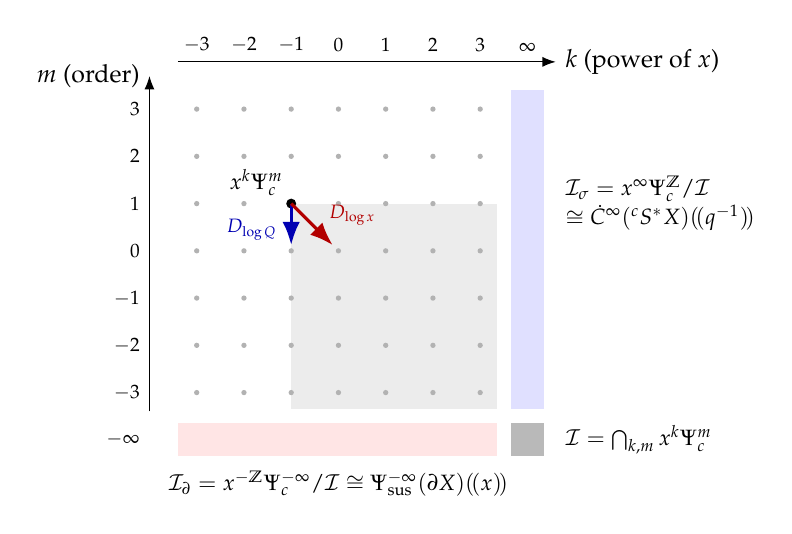
\begin{tikzpicture}[>=Latex,scale=0.6]
 \fill[gray!15] (-1,1) rectangle (3.35,-3.35);
 \fill[blue!12] (3.65,-3.35) rectangle (4.35,3.4);
 \fill[red!10] (-3.4,-3.65) rectangle (3.35,-4.35);
 \fill[gray!55] (3.65,-3.65) rectangle (4.35,-4.35);
 \foreach \k in {-3,...,3}{\foreach \m in {-3,...,3}{\fill[gray!60] (\k,\m) circle (1.6pt);}}
 \draw[->] (-3.4,4.0)--(4.6,4.0) node[right] {\small \(k\) (power of \(x\))};
 \draw[->] (-4.0,-3.4)--(-4.0,3.7) node[left] {\small \(m\) (order)};
 \foreach \k in {-3,...,3} \node[font=\scriptsize,above] at (\k,4.0) {\(\k\)};
 \node[font=\scriptsize,above] at (4,4.0) {\(\infty\)};
 \foreach \m in {-3,...,3} \node[font=\scriptsize,left] at (-4.0,\m) {\(\m\)};
 \node[font=\scriptsize,left] at (-4.0,-4) {\(-\infty\)};
 \fill (-1,1) circle (3pt);
 \node[font=\footnotesize,anchor=south east,fill=white,inner sep=1pt] at (-1.1,1.1) {\(x^k\Psic^m\)};
 \draw[->,very thick,blue!70!black] (-1,1)--(-1,0.12);
 \node[font=\scriptsize,blue!70!black,anchor=east] at (-1.1,0.45) {\(D_{\lQ}\)};
 \draw[->,very thick,red!70!black] (-1,1)--(-0.12,0.12);
 \node[font=\scriptsize,red!70!black,anchor=west] at (-0.4,0.75) {\(D_{\lx}\)};
 \node[font=\footnotesize,align=left,anchor=west] at (4.6,1.0)
   {\(\Is=x^\infty\Psic^{\Z}/\cI\)\\[1pt] \(\cong\dCI(\Y)\Lser{q^{-1}}\)};
 \node[font=\footnotesize,anchor=north] at (0,-4.45)
   {\(\Id=x^{-\Z}\Psic^{-\infty}/\cI\cong\Psis^{-\infty}(\partial X)\Lser{x}\)};
 \node[font=\footnotesize,anchor=west] at (4.6,-4.0) {\(\cI=\bigcap_{k,m}x^k\Psic^m\)};
\end{tikzpicture}
\caption[The two filtrations and the residual ideals]{The two filtrations
of \(x^{-\Z}\Psic^{\Z}(X)\). The dot at \((k,m)\) stands for
\(x^k\Psic^m(X)\), which contains \(x^{k'}\Psic^{m'}(X)\) for \(k'\ge k\)
and \(m'\le m\) (shaded, for \((k,m)=(-1,1)\)). Every element lies in such a
quadrant: powers of \(x\) are bounded below, as in \(\Lser{x}\), and orders
are bounded above, as in \(\Lser{q^{-1}}\). The residual edges are
\(k=\infty\), giving \(\Is\) (blue), and \(m=-\infty\), giving \(\Id\)
(red); the corner \(\cI\) is divided out, so \(\Is\cap\Id=0\) in \(\cA\).
Then \(\As=\cA/\Id\) forgets the bottom edge, \(\Ad=\cA/\Is\) the right
edge, and \(\Ads\) both. Arrows: on symbols \(D_{\lQ}\) lowers the order by
one, and \(D_{\lx}\) lowers the order by one and raises the power of \(x\)
by one (Section~\ref{sec:derivations}).}
\label{fig:lattice}
\end{figure}

\subsection{The main homological results}\label{subsec:mainresults}
Write \(Y=\Y\) for the cosphere bundle of the cusp cotangent bundle; it
is a compact manifold with boundary of dimension \(2n-1\), and its
boundary is \(Z=\Zb\), the part over \(\partial X\). Let \(\Ssig\) and
\(\Sd\) be circles. They record the homogeneity in the fibres and the
Laurent variable \(x\), and carry the classes \(d\theta_\sigma=[d\log r]\)
and \(d\theta_\partial=[d\log x]\). All cohomology has complex
coefficients, and Hochschild homology is the continuous homology of
Section~\ref{sec:hhtools}.

MN state their results for Hochschild \emph{cohomology}
\cite[(16)]{MN}. In the form proved in these notes they read as follows.

\begin{theorem}[MN (16), with the number of boundary components restored]
\label{thm:main}
Let \(X\) be connected, \(n=\dim X\ge2\), and let \(\partial X\) have
\(N\ge1\) components \(H_1,\dots,H_N\). Then \(Y\) is connected, and
\(Z=\bigsqcup_jZ_j\) with each \(Z_j={}^cS^*_{H_j}X\) connected. The
continuous Hochschild cohomology groups are:
\begin{align*}
 \HH^k(\cI)&\cong\begin{cases}\C,&k=0,\\0,&k>0,\end{cases}\\
 \HH^k(\Is)&\cong H^k(Y\times\Ssig),\\
 \HH^k(\As)&\cong\Hrel^k(Y\times\Ssig)\oplus H^k(Z\times\Ssig),\\
 \HH^k(\Ads)&\cong H^k(Z\times\Ssig\times\Sd),\\
 \HH^k(\Id)&\cong\begin{cases}\C^N,&k=0,1,\\0,&k\ge2,\end{cases}\\
 \HH^k(\Ad)&\cong\begin{cases}H^k(Z\times\Ssig\times\Sd)/\C^N,&k=1,2,\\
 H^k(Z\times\Ssig\times\Sd),&\text{otherwise,}\end{cases}\\
 \HH^k(\cA)&\cong\begin{cases}
 \C\oplus\Hrel^1(Y\times\Ssig)\oplus H^1(Z\times\Ssig)/\C^N,&k=1,\\
 \bigl(\Hrel^2(Y\times\Ssig)\oplus H^2(Z\times\Ssig)\bigr)/\C^{N-1},&k=2,\\
 \Hrel^k(Y\times\Ssig)\oplus H^k(Z\times\Ssig),&\text{otherwise.}
 \end{cases}
\end{align*}
The subspaces \(\C^N\) are spanned by the classes \(d\theta_\sigma\cdot
1_{Z_j}\) (for \(k=1\)) and \(d\theta_\partial\wedge d\theta_\sigma\cdot
1_{Z_j}\) (for \(k=2\)), and \(\C^{N-1}\) is the image of
\(\{\sum_jc_j\,d\theta_\sigma1_{Z_j}\}\) under the de Rham connecting map
\(H^1(Z\times\Ssig)\to\Hrel^2(Y\times\Ssig)\); it is
\((N-1)\)-dimensional. Finally \(\HH^k(x^{-\Z}\Psic^{\Z}(X))\cong
\HH^k(\cA)\) for \(k\ne1\), while \(\HH^1(x^{-\Z}\Psic^{\Z}(X))\) is the
quotient of \(\HH^1(\cA)\) by the line spanned by the index cocycle.
\end{theorem}

For \(N=1\) these are exactly the formulas of \cite[(16)]{MN}. The
corresponding homology groups are obtained by Lefschetz duality on the
\(2n\)-manifold \(Y\times\Ssig\) and Poincar\'e duality on the closed
manifolds \(Z\times\Ssig\) and \(Z\times\Ssig\times\Sd\). For example
\cite[Props.~2, 3]{MN}
\[
 \HH_k(\Is)\cong\Hrel^{2n-k}(Y\times\Ssig),\qquad
 \HH_k(\As)\cong H^{2n-k}(Y\times\Ssig)\oplus H^{2n-k-1}(Z\times\Ssig).
\]
The precise sources of the hypotheses are discussed in
Corrections~\ref{corr:components} and~\ref{corr:n1}. The proof rests on
one quoted input, the last step of the convergence for \(\Ads\), or
equivalently for \(\As\) (B10; Proposition~\ref{ha:prop:equiv}). This
step is proved for \(n=1\) (Corollary~\ref{ha:cor:n1}) but not for the
case \(n\ge2\) of Theorem~\ref{thm:main}. The boundary connecting map (B9)
is proved (Theorem~\ref{ha:thm:bdry}), and everything else the proof uses
is proved in the appendices (Section~\ref{subsec:background}), except
Lemma~\ref{ha:lem:mixed}(b), whose proof is sketched after \cite{HHb}. The proof
of Theorem~\ref{thm:main} occupies
Sections~\ref{sec:functions}--\ref{sec:AdA}.

\subsection{The index formula}\label{subsec:indexintro}
A matrix \(A\) of elements of \(x^{-\Z}\Psic^{\Z}(X)\) is \emph{fully
elliptic} if its image in (a matrix algebra over) \(\cA\) is invertible,
with the orders matched: for \(A\in x^{-p}\Psic^m\) the inverse is the
class of an element of \(x^p\Psic^{-m}\) (Theorem~\ref{cc:thm:parametrix}).
For an operator of order \(m\) this means two things: \(A\) is elliptic as
a cusp operator, and its indicial family \(\In(A,\tau)\) is invertible for
every real \(\tau\). Such an operator is Fredholm on \(\dCI(X)\), and
Fedosov's formula reads \cite[(7)]{MN}
\begin{equation}\label{eq:fedosovintro}
 \Ind(A)=\dim\ker A-\dim\ker A^*=\Tr([A,B])=\IF([A],[A]^{-1}),
\end{equation}
where \(B\) is any inverse of \(A\) modulo \(\cI\). The \emph{index
functional} \(\IF\) is the image of the trace on \(\cI\) under the
connecting map of \(0\to\cI\to x^{-\Z}\Psic^{\Z}(X)\to\cA\to0\). MN
express it through the following data:
\begin{itemize}
\item the extensions \(\hTrd\) and \(\hTrs\) of the traces on the two
ideals \(\Id\) and \(\Is\);
\item the two exterior derivations \(D_{\lx}=[\lx,\cdot\,]\) and
\(D_{\lQ}=[\lQ,\cdot\,]\).
\end{itemize}
In the form proved here (Proposition~\ref{prop:IF}),
\begin{equation}\label{eq:IFintro}
 \IF(A,B)=\tfrac12\bigl(\hTrd+\hTrs\bigr)\bigl(B\widetilde D(A)+
 \widetilde D(A)B\bigr),\qquad \widetilde D=[\lx-\lQ,\cdot\,].
\end{equation}
This is \cite[(87)]{MN}. In \cite[(21)]{MN} the derivation is printed with
the opposite sign (Correction~\ref{corr:Dtilde}). Inserting \(B=A^{-1}\)
splits the index into four terms. If \(A\) is translation invariant near the
boundary with normal indicial family, two of them vanish, and one obtains
the pseudodifferential APS formula (Theorem~\ref{thm:reduced}):
\begin{equation}\label{eq:reducedintro}
 \Ind(A)=\AS(A)-\tfrac12\etab(A),\qquad
 \AS(A)=\TrR\bigl(A[\lQ,A^{-1}]\bigr),\qquad
 \etab(A)=\eta(A_0)+\delta_Q(A).
\end{equation}
Here \(A_0=\In(A)\), \(t=1/x\) is the suspension variable,
\(\eta(A_0)=2\,\bTr\bigl(A_0^{-1}[t,A_0]\bigr)\), \(\bTr\) is
Melrose's regularized trace on the suspended algebra, and in terms of the
indicial variable
\[
 \eta(A_0)=\frac1{\pi i}\,\overline{\int_{\R}}\Tr\Bigl(A_0(\tau)^{-1}
 \frac{dA_0(\tau)}{d\tau}\Bigr)\,d\tau .
\]
The term \(\delta_Q(A)\) is a local functional of the boundary symbols of
\(A\) and \(Q\). It comes from the corrected form of \cite[Prop.~8]{MN}
(item~\ref{item:Prop8reg} of Section~\ref{subsec:errata}), and it vanishes
in the cases treated in Section~\ref{sec:examples}
(Proposition~\ref{prop:eta}). For a Dirac operator in APS normal form
\(\eta(A_0)\) is the Atiyah--Patodi--Singer
eta invariant of the boundary operator (Corollary~\ref{cor:Dirac}). In MN,
\cite[(22)--(24)]{MN} and \cite[(100)]{MN}, the Atiyah--Singer term is
written \(\TrR(A^{-1}[\lQ,A])\), which is \(-\AS(A)\). The sign is wrong;
see Correction~\ref{corr:ASsign} and the checks in
Section~\ref{sec:examples}.

\subsection{Organization and how to read these notes}
Section~\ref{sec:conventions} fixes conventions and gives the dictionary to
MN's notation. It also lists the background facts, with the appendix
results that prove them and what remains quoted, and it collects the
corrections. Section~\ref{sec:closed} treats the closed case
(Brylinski--Getzler, Wodzicki), which is the template for everything else.
Section~\ref{sec:cusp} introduces the cusp calculus, starting from the
half-line. Section~\ref{sec:hhtools} assembles the homological toolkit.
Sections~\ref{sec:functions}--\ref{sec:AdA} follow \cite[\S\S1--8]{MN} and
prove Theorem~\ref{thm:main}. Sections~\ref{sec:morita}--\ref{sec:index}
follow \cite[\S\S9--12]{MN} and prove the index formula.
Section~\ref{sec:examples} contains worked examples.
Section~\ref{sec:other} summarizes \cite[\S\S13--15]{MN}.
Section~\ref{sec:comparison} compares the cusp and b-calculi and cites the
companion notes \cite{HHb}. Appendices~\ref{cc:sec:cusp}--\ref{tr:sec}
prove the background facts (B1)--(B10) of Section~\ref{subsec:background},
apart from the inputs listed there as quoted. The main text can be read
without them: each step that uses a background fact names the appendix
result that proves it.

Figure~\ref{fig:roadmap} shows the logical dependencies.

\begin{figure}[htbp]
\centering
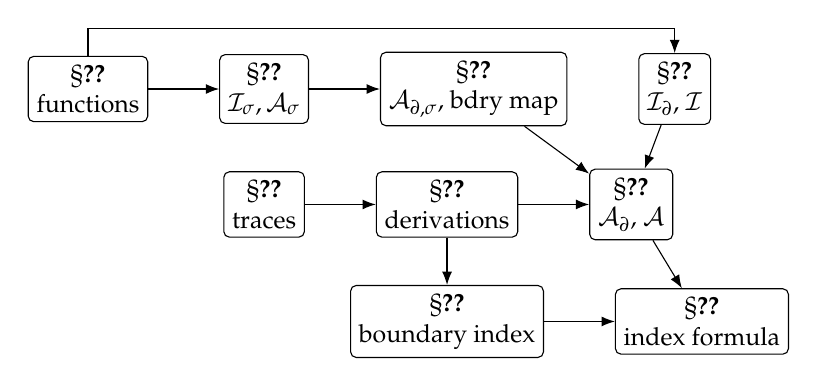
\begin{tikzpicture}[>=Latex,node distance=6mm and 9mm,
  box/.style={draw,rounded corners=2pt,align=center,font=\small,
  inner sep=3pt,minimum height=7mm}]
 \node[box] (fun) {\S\ref{sec:functions}\\ functions};
 \node[box,right=of fun] (sym) {\S\ref{sec:symbols}\\ \(\Is,\As\)};
 \node[box,right=of sym] (bdy) {\S\ref{sec:boundarysym}\\ \(\Ads\), bdry map};
 \node[box,right=of bdy] (ind) {\S\ref{sec:indicial}\\ \(\Id\), \(\cI\)};
 \node[box,below=of sym] (tr) {\S\ref{sec:residues}\\ traces};
 \node[box,right=of tr] (der) {\S\ref{sec:derivations}\\ derivations};
 \node[box,right=of der] (AdA) {\S\ref{sec:AdA}\\ \(\Ad\), \(\cA\)};
 \node[box,below=of der] (bi) {\S\ref{sec:boundaryindex}\\ boundary index};
 \node[box,right=of bi] (IF) {\S\ref{sec:index}\\ index formula};
 \draw[->] (fun)--(sym); \draw[->] (sym)--(bdy); \draw[->] (fun.north) -- ++(0,0.35) -| (ind.north);
 \draw[->] (bdy)--(AdA); \draw[->] (ind)--(AdA);
 \draw[->] (tr)--(der); \draw[->] (der)--(AdA);
 \draw[->] (der)--(bi); \draw[->] (bi)--(IF); \draw[->] (AdA)--(IF);
\end{tikzpicture}
\caption[Logical structure of the notes]{Logical structure of the main
part of the notes.}
\label{fig:roadmap}
\end{figure}

\section{Conventions, dictionary, background and corrections}
\label{sec:conventions}

\subsection{Coordinates and Fourier conventions}\label{subsec:coords}
Near a boundary point we use coordinates \((x,y)\), \(y\in\R^{n-1}\),
where \(x\) is the fixed boundary defining function. The \emph{cusp
cotangent} coordinates \((x,y,\tau,\eta)\) are defined by writing a cusp
covector as
\begin{equation}\label{eq:cuspcovector}
 \alpha=\tau\,\frac{dx}{x^2}+\eta\cdot dy ,
\end{equation}
as in \cite[(139)]{MN}. Thus \(\tau\) is the symbol of \(x^2D_x\), where
\(D=-i\partial\). The canonical symplectic form is
\(\omega=d\alpha=d\tau\wedge\frac{dx}{x^2}+\sum_jd\eta_j\wedge dy_j\). It
agrees with the standard form \(\sum d\xi\wedge dx\) in the interior, where
\(\tau=x^2\xi\). The Poisson bracket is
\begin{equation}\label{eq:poisson}
 \{a,b\}=\partial_\tau a\,x^2\partial_xb-x^2\partial_xa\,\partial_\tau b
 +\partial_\eta a\cdot\partial_yb-\partial_ya\cdot\partial_\eta b ,
\end{equation}
and the principal symbol of a commutator is
\(\sigma([A,B])=-i\{\sigma(A),\sigma(B)\}\). (In \cite[(139)]{MN} the
last term is misprinted as \(\partial_ya\cdot\partial_\tau b\).)
Formula \eqref{eq:poisson} follows from the usual bracket
\(\partial_\xi a\,\partial_xb-\partial_xa\,\partial_\xi b\) by the change of
variables \(\tau=x^2\xi\). Indeed \(\partial_\xi|_x=x^2\partial_\tau\) and
\(\partial_x|_\xi=\partial_x|_\tau+2x^{-1}\tau\,\partial_\tau\), and the two
terms involving \(2x^{-1}\tau\) cancel.

Near the boundary we use the \emph{suspension variable}
\begin{equation}\label{eq:t}
 t=\frac1x\in(1,\infty),\qquad x^2\partial_x=-\partial_t,\qquad
 \frac{dx}{x^2}=-dt .
\end{equation}
Fourier transformation is \(\hat u(\xi)=\int e^{-it\xi}u(t)\,dt\), with
inverse \(u(t)=(2\pi)^{-1}\int e^{it\xi}\hat u(\xi)\,d\xi\), as in the
companion notes \cite{Notes,HHb}.

\subsection{The indicial variable}\label{subsec:indicialvariable}
MN define the indicial family by conjugation \cite[Def.~4]{MN}:
\begin{equation}\label{eq:Indef}
 \In(A,\tau)=\Bigl(e^{i\tau/x}Ae^{-i\tau/x}\Bigr)\Big|_{\partial X},
 \qquad\tau\in\R .
\end{equation}
Then \(\In(x^2D_x,\tau)=\tau\), so the indicial variable is the boundary
value of the cusp covariable of \eqref{eq:cuspcovector}. For a translation
invariant operator on \(\R_t\times\partial X\) with convolution kernel
\(\kappa(t-t',y,y')\), one finds
\begin{equation}\label{eq:Inkernel}
 \In(A,\tau)=\int_{\R}e^{i\tau s}\kappa(s,\cdot,\cdot)\,ds=\hat\kappa(-\tau),
 \qquad \In(D_t,\tau)=-\tau,\qquad
 \In([t,A],\tau)=-i\,\partial_\tau\In(A,\tau).
\end{equation}
The last identity holds because \([t,A]\) has kernel
\((t-t')\kappa(t-t')\). Under the transcendental blow-up \(x_b=e^{-1/x}\)
of Section~\ref{subsec:transcendental}, the b-indicial family of the
companion notes, \(I(A,\lambda)=\int e^{-iz\lambda}\kappa_A(e^z)\,dz\) with
\(z=\log(x_b/x_b')=-(t-t')\), becomes \eqref{eq:Inkernel} with
\(\tau=\lambda\). So \emph{the cusp indicial variable \(\tau\) of MN is
the b-indicial variable \(\lambda\) of \cite{Notes,HHb}}. In the b-calculus
\(\lambda\) may be complex. In the cusp calculus only real \(\tau\) occurs.

\subsection{Densities and traces}\label{subsec:traces}
Kernels are taken with respect to a cusp density \(\nu_c\) in the right
variable, equal to \(x^{-2}dx\,\nu_\partial=dt\,\nu_\partial\) near the
boundary, where \(\nu_\partial\) is a smooth positive density on
\(\partial X\). This is the convention of Appendix~\ref{cc:sec:cusp}; MN
normalize kernels as cusp half-densities \cite[(118)]{MN}, which gives
the same operator spaces (Section~\ref{subsec:double}). We use
the following functionals; complex parameters are written \(s\) (for
powers of \(Q\)) and \(z\) (for powers of \(x\)).
\begin{center}
\renewcommand{\arraystretch}{1.25}
\begin{tabular}{lll}
 functional & definition & MN\\\hline
 \(\Tr\) on \(\cI\) & integral of the kernel on the diagonal & \(\Tr\)\\
 \(\Trs\) on \(\Is\) & \(\Res_{s=0}\Tr(AQ^{-s})\) (Wodzicki residue) & (49)\\
 \(\Trd\) on \(\Id\) & \(\Res_{z=0}\Tr(Ax^z)\) & Lemma 10\\
 \(\Trds\) on \(\cA\) & coefficient of \((sz)^{-1}\) in \(Z(A;s,z)\) & (44)\\
 \(\hTrs\), \(\hTrd\) & the mixed coefficients of \(Z(A;s,z)\) & (44)\\
 \(\bTr\) on \(\Psis^{\Z}(\partial X)\) &
 \((2\pi)^{-1}\overline{\int}\Tr\In(B,\tau)\,d\tau\) & (57)--(59)\\
\end{tabular}
\end{center}
Here \(Z(A;s,z)=\frac12\bigl(\Tr(Ax^zQ^{-s})+\Tr(AQ^{-s}x^z)\bigr)\).
\textbf{MN write \(\tau\) for our \(s\)} in \cite[(43)--(62)]{MN}, and also
use \(\tau\) for the cusp covariable in \cite[(139)]{MN}. We keep \(\tau\)
for the covariable throughout.

\subsection{Hochschild conventions}
The Hochschild boundary is
\(b=\sum_{i=0}^k(-1)^id_i\), where \(d_i\) multiplies \(a_i\) and
\(a_{i+1}\) for \(i<k\) and \(d_k(a_0\otimes\dots\otimes a_k)=a_ka_0\otimes
a_1\otimes\dots\otimes a_{k-1}\). The bar differential is
\(b'=\sum_{i<k}(-1)^id_i\). For a derivation \(D\),
\[
 i_D(a_0\otimes a_1\otimes\dots\otimes a_k)=a_0D(a_1)\otimes a_2\otimes
 \dots\otimes a_k \qquad\text{\cite[\S6]{MN}},
\]
and on cochains \(i_D\varphi=\varphi\circ i_D\). For a \(0\)-cochain
\(\varphi\) this reads
\[
 (i_D\varphi)(A,B)=\varphi\bigl(AD(B)\bigr).
\]

\subsection{Background facts: where they are proved}\label{subsec:background}
The paper \cite{MN} quotes the analytic foundations of the cusp calculus
and the homological tools. Appendices~\ref{cc:sec:cusp}--\ref{tr:sec}
prove most of them. For each item we state the fact as it is used, say
which appendix result proves it, and record what remains quoted. Every
step in the main text that uses one of these facts says so.
\begin{enumerate}
\item[(B1)] \emph{Cusp calculus.} The cusp operators form a doubly filtered
\(*\)-algebra, and conjugation by \(x^z\) preserves both filtrations. There
are the symbol sequence \cite[(11)]{MN}, the indicial sequence
\cite[(12)]{MN}, a global quantization map \cite[Prop.~24]{MN}, which
gives the \emph{linear} isomorphisms \cite[(13)]{MN}, and the Taylor series
isomorphism at the front face \cite[Prop.~25]{MN}, which is an algebra
isomorphism for the twisted product. \emph{Proved}:
Theorem~\ref{cc:thm:comp}, Propositions~\ref{cc:prop:symbol},
\ref{cc:prop:indicial}, \ref{cc:prop:quant}, \ref{cc:prop:taylor},
\ref{cc:prop:conj}; agreement with \cite[Def.~2]{MN} is
Proposition~\ref{cc:prop:MNdef}, and the lift of b-operators
\cite[Prop.~26]{MN} is Proposition~\ref{cc:prop:transcendental}.
\emph{Quoted}: the standard uniform pseudodifferential calculus on the
cylinder \(\R\times\partial X\) (Background fact~\ref{cc:bg:uniform}), and
the density half of \cite[Prop.~26]{MN} (Remark~\ref{cc:rem:density}),
which is not used.
\item[(B2)] \emph{Fredholm theory.} A fully elliptic element of
\(x^{-p}\Psic^m(X;E)\) has an inverse modulo \(\cI\) in
\(x^p\Psic^{-m}(X;E)\). It is Fredholm on \(\dCI(X;E)\) and on the cusp
Sobolev spaces, its kernel and cokernel lie in \(\dCI\), and it has a
generalized inverse in the calculus \cite[p.~4, \S12]{MN}. \emph{Proved}:
Theorems~\ref{cc:thm:parametrix} and~\ref{cc:thm:fredholm}.
\item[(B3)] \emph{Holomorphic families and meromorphy.} \cite[Lemma~4,
App.~B]{MN} use the complex powers \(Q^{-s}\) of a positive elliptic
\(Q\in\Psic^1(X)\), and the meromorphy of \(\Tr(A(s,z)x^zQ^{-s})\), with at
most simple poles on the lines \(s=m+n-k\) and \(z=-p+1-j\). \emph{Proved}
in the form (B3\('\)) of Appendix~\ref{tr:sec}: any admissible family
\(Q(s)\) of order \(-s\) with \(Q(0)=\mathrm{Id}\) may replace \(Q^{-s}\)
(Proposition~\ref{tr:prop:Q} constructs one explicitly);
Theorem~\ref{tr:thm:mero} proves the two-variable meromorphy and identifies
the residues, and Proposition~\ref{tr:prop:transfer} shows which results
of Sections~\ref{sec:residues}--\ref{sec:index} hold for such families. In
the main text \(Q^{-s}\) may be read as any admissible family, with the
single change noted after Proposition~\ref{prop:IF}. \emph{Quoted
(sketched)}: the cusp calculus with holomorphic parameters
(Lemmas~\ref{tr:lem:holcalc}(1) and~\ref{tr:lem:cuspcalc}).
\item[(B4)] \emph{Wodzicki excision.} A short exact sequence of
topological algebras whose kernel is topologically H-unital gives a long
exact sequence in continuous Hochschild homology \cite{Wodzicki}.
\emph{Proved}: Theorem~\ref{ha:thm:excision}, with
Lemma~\ref{ha:lem:exact} for the exactness of the chain spaces.
\emph{Quoted}: the facts (F1)--(F3) about nuclear Fr\'echet spaces
\cite{Treves}.
\item[(B5)] \emph{Connes' theorem.} The Hochschild--Kostant--Rosenberg map
gives \(\HH_k(\CI(M))\cong\CI(M;\Lambda^k)\) for compact manifolds,
possibly with boundary or corners, and similarly for the formal, Laurent,
flat and Schwartz coefficient algebras \cite{Connes}. \emph{Proved}:
Theorems~\ref{ha:thm:connes} and~\ref{ha:thm:variants}, and
Corollary~\ref{ha:cor:homog} for homogeneous functions.
\item[(B6)] \emph{K\"unneth and Morita.} The K\"unneth formula in the
form used, and Morita invariance for matrices, smoothing-kernel algebras
and full corners \(eM_N(\mathfrak A)e\) \cite{Connes,Loday}. \emph{Proved}:
Proposition~\ref{ha:prop:kunneth} and Corollary~\ref{ha:cor:homog}
(K\"unneth); Lemma~\ref{ha:lem:morita}, Proposition~\ref{ha:prop:corner}
and Remark~\ref{ha:rem:bundles} (Morita). \emph{Quoted}: the
Eilenberg--Zilber theorem (Background fact~\ref{ha:bg:EZ}); and Morita
invariance for the H-unital ideals with bundle coefficients, which is only
sketched in Remark~\ref{ha:rem:bundles}. The topological K\"unneth formula
of \cite{Karoubi} is not needed.
\item[(B7)] \emph{The suspended algebra} \cite{MelroseEta}. The
regularized trace \(\bTr\) is a trace on \(\Psis^{\Z}\); its regularization
by a holomorphic family carries a local correction (this corrects
\cite[Prop.~8]{MN}); the eta invariant
\(\eta(A)=(\pi i)^{-1}\overline{\int}\Tr(A^{-1}\partial_\tau A)\,d\tau\)
is the APS eta invariant for Dirac operators; and \(\etab=\eta(A_0)+
\delta_Q\). \emph{Proved}: Theorems~\ref{tr:thm:bTr},
\ref{tr:thm:susreg}, \ref{tr:thm:Dirac} and
Proposition~\ref{tr:prop:etabar}(i). \emph{Quoted}: in
Theorem~\ref{tr:thm:Dirac}, the small-time heat expansion and the
regularity of \(\eta_B(s)\) at \(s=0\) from \cite{Notes}; in
Proposition~\ref{tr:prop:etabar}(ii), the fact that
\((D_t^2+B^2)^{-s/2}\) is an entire suspended family (Seeley's complex
powers with a parameter \cite{Seeley}); the parity argument of
Remark~\ref{tr:rem:parity} (sketch); and, in Remark~\ref{tr:rem:plusone},
the local cancellation of Bismut--Freed \cite{BismutFreed}.
\item[(B8)] \emph{Wodzicki residue} \cite{Wodzicki-residue,Guillemin-residue}:
it is a trace, given by the local formula
\((2\pi)^{-n}\int_{S^*M}a_{-n}\,\nu\), independent of \(Q\), and for
\(n\ge2\) unique among traces vanishing on smoothing operators.
\emph{Proved}: Theorem~\ref{tr:thm:res} and
Proposition~\ref{tr:prop:unique}. \emph{Quoted, not used}: Wodzicki's
stronger uniqueness, that every trace on \(\Psi^{\Z}\) vanishes on
\(\Psi^{-\infty}\).
\item[(B9)] \emph{The boundary connecting map} \cite[Prop.~5]{MN}: part
(3) of Proposition~\ref{prop:boundaryLES}, i.e.\ that the connecting map
\(\HH_k(\Ads)\to\HH_{k-1}(\Is)\) is a non-zero universal multiple of the
de Rham connecting map on the summand without \(d\theta_\partial\) and
vanishes on the other summand. MN's proof uses a multiplicative splitting
\(s_0\) that we could not reconstruct (Remark~\ref{rem:s0}).
\emph{Proved} without it: Lemma~\ref{ha:lem:connlead} computes the leading
part of a connecting map with a linear lift, and
Theorem~\ref{ha:thm:bdry} gives \(\Theta_{\Is}\circ\partial=(-1)^ki\,
(\delta_{\mathrm{dR}}\oplus0)\circ\Theta_{\partial,\sigma}\) for the
leading-symbol maps, with no convergence hypothesis. Read as a statement
about the isomorphisms of Propositions~\ref{prop:Is} and~\ref{prop:Ads},
it needs \(\Theta_{\partial,\sigma}\) to be an isomorphism, which is (B10).
\item[(B10)] \emph{Convergence for the Laurent symbol algebras.} The order
spectral sequences of \(\As\) and \(\Ads\) converge, so that
\(\HH_k\) is isomorphic to \(E^2_{k-n,k}\) by the leading symbol.
\emph{Proved}: the algebraic convergence statement
(Proposition~\ref{ha:prop:algconv}), completeness through mixed complexes
(Lemma~\ref{ha:lem:mixed}; part (b) is sketched after \cite{HHb}), convergence for the closed symbol algebra and
for \(\Is\) (Theorem~\ref{ha:thm:conv}), the partial result
Proposition~\ref{ha:prop:laurent} for \(\As\) and \(\Ads\), the
equivalence of the statements for \(\As\) and for \(\Ads\)
(Proposition~\ref{ha:prop:equiv}), and both statements for \(n=1\)
(Proposition~\ref{ha:prop:xadic}, Corollary~\ref{ha:cor:n1}). The stage
argument used for the b-calculus in \cite{HHb} fails here, because the
cusp Lie derivative \(\mathcal L_{x^2\partial_x}\) is nilpotent on leading
coefficients (Example~\ref{ha:ex:obstruction}). For \(n\ge2\) neither the
\(x\)-adic filtration (Remark~\ref{ha:rem:xadicfail}) nor the theorem of
Benameur--Nistor \cite{BN} (Remark~\ref{ha:rem:BN}) closes the gap.
\emph{Quoted}, for \(n\ge2\): the remaining step, from \cite[p.~12]{MN}
(Remark~\ref{ha:rem:quoted}). The analogous question for the \(x\)-adic
spectral sequence of \(\Id\) is settled: Proposition~\ref{ha:prop:Idconv}
proves its convergence.
\end{enumerate}
In summary, the following remain quoted or only sketched:
\begin{itemize}
\item (B10) for \(n\ge2\): the last step of the convergence for \(\Ads\),
equivalently for \(\As\) (Remark~\ref{ha:rem:quoted},
Proposition~\ref{ha:prop:equiv});
\item Lemma~\ref{ha:lem:mixed}(b), the comparison of mixed complexes,
sketched after \cite{HHb}; Theorems~\ref{ha:thm:conv} and~\ref{ha:thm:bdry} (through \(\Theta_{\Is}\)),
Proposition~\ref{ha:prop:xadic} and Proposition~\ref{ha:prop:Idconv}
use it;
\item the uniform calculus on cylinders (Background
fact~\ref{cc:bg:uniform});
\item the nuclear-space facts (F1)--(F3) of Appendix~\ref{ha:sec};
\item the Eilenberg--Zilber theorem (Background fact~\ref{ha:bg:EZ});
\item Morita invariance for the H-unital ideals with bundle coefficients
(sketched in Remark~\ref{ha:rem:bundles});
\item the calculus with holomorphic parameters
(Lemmas~\ref{tr:lem:holcalc}(1) and~\ref{tr:lem:cuspcalc}, sketched);
\item the inputs of the eta identification: the heat expansion and the
regularity of \(\eta_B\) in Theorem~\ref{tr:thm:Dirac} \cite{Notes}, the
entire suspended family in Proposition~\ref{tr:prop:etabar}(ii)
\cite{Seeley}, the parity sketch of Remark~\ref{tr:rem:parity}, and
Bismut--Freed in Remark~\ref{tr:rem:plusone} \cite{BismutFreed};
\item Wodzicki's stronger uniqueness of the residue (not used);
\item the density half of \cite[Prop.~26]{MN} (Remark~\ref{cc:rem:density};
not used).
\end{itemize}

\subsection{Corrections and unstated hypotheses}\label{subsec:errata}
For convenience we list here the points where we disagree with the text of
\cite{MN}. Each is proved in the place indicated.
\begin{enumerate}
\item \emph{Connected boundary.} \cite[(16)]{MN}, Proposition~6,
Lemma~12 and Proposition~12 treat \(\Id\) as if \(\partial X\) were connected.
For \(N\) components, \(\HH^0(\Id)\cong\HH^1(\Id)\cong\C^N\), the
double residue splits into \(N\) traces, and the boundary map
\(\HH^1(\Id)\to\HH^2(\As)\) has rank \(N-1\)
(Correction~\ref{corr:components}).
\item \emph{Dimension one.} For \(n=1\) the boundary cosphere bundle
\(Z_j\) consists of two points. Then the residue traces \(\Tr_\sigma\)
and \(\Tr_{\partial,\sigma}\) split into two (Correction~\ref{corr:n1});
the boundary trace \(\Tr_\partial\) on \(\Id\) does not, and the claims ``\(\HH^0\) is
one-dimensional'' fail.
\item \emph{The cusp de Rham complex.} The remark after \cite[(33)]{MN}
says that the cusp de Rham complex has b-cohomology. In fact it has an
extra summand \(H^{k-1}(\partial M)\) (Correction~\ref{corr:cdR}). This is
not used elsewhere.
\item \emph{The cut-off in Lemma~1.} The function \(\phi\) in \cite[(26)]{MN}
must be supported in \((-1,1)\) (Remark~\ref{rem:phi}).
\item \emph{The derivation \(\widetilde D\).} \cite[(21)]{MN} and
\cite[(83)]{MN} have opposite signs; \eqref{eq:IFintro} is correct
(Correction~\ref{corr:Dtilde}).
\item \emph{Signs of \(\bAS\) and \(\beta\) in \cite[(93)]{MN}.} With the
definitions \cite[(90), (91)]{MN} the index theorem reads
\(\Ind=-\bAS-\frac12\etab-\beta_Q+\gamma\). The symbolic term in
\cite[(23), (100)]{MN} has the wrong sign (Correction~\ref{corr:ASsign}).
\item \emph{The eta term.} The last line of the proof of
\cite[Prop.~17]{MN} should read \(\etab(A)=2\bTr(A_0^{-1}[t,A_0])\).
The proposition needs \(Q\) to be asymptotically translation invariant
(Correction~\ref{corr:eta}), and by item~\ref{item:Prop8reg} its
conclusion becomes \(\etab(A)=\eta(A_0)+\delta_Q(A)\).
\item \emph{The residue on the suspended algebra.} The identification of the
residue with \(\bTr([t,B])\) in \cite[Prop.~8]{MN} fails, for instance when
\(\partial X\) is a point (Remark~\ref{rem:Prop8}); a parity argument
of the same kind applies to \(Q_0^{-n}\) on any boundary. We use the residue
itself.
\item\label{item:Prop8reg} \emph{The regular value in MN Proposition~8.}
\cite[Prop.~8]{MN} also asserts that the regular value at \(s=0\) of
\(\bTr(BQ_0^{-s})\) is \(\bTr(B)\). This is false in general: for
\(\partial X\) a point and \(B=\langle D_t\rangle\) the two differ by
\(-1/2\pi\) (Example~\ref{tr:ex:counter}). The regular value is
\(\bTr(B)+\gamma'(0)/2\pi\), with a local correction \(\gamma'(0)\)
(Theorem~\ref{tr:thm:susreg}, Correction~\ref{tr:corr:Prop8}). The error
propagates to \cite[Cor.~2]{MN}, which acquires the correction term
(Corollary~\ref{cor:Tr61}(2)), and to \cite[Prop.~17]{MN}, which becomes
\(\etab(A)=\eta(A_0)+\delta_Q(A)\) with \(\delta_Q\) local
(Proposition~\ref{prop:eta}). The correction \(\delta_Q\) vanishes in the
cases used in Section~\ref{sec:examples}, including the interval example
(Example~\ref{ex:interval-index}). It is compensated by \(\beta_Q\) in
general, since the index does not depend on \(Q\).
\item \emph{The compactification in Appendix A.} The map
\cite[(130)]{MN} gives \([-1,1]\) the wrong smooth structure at the
endpoints for the cusp calculus. One must compactify by \(1/z\)
(Remark~\ref{rem:SP}).
\item \emph{The cusp metric in Appendix B.} The metric
\(dx^2/x^4+h/x^2\) of \cite[App.~B]{MN} is a scattering metric, and its
Laplacian is not cusp-elliptic. An exact cusp metric is
\(dx^2/x^4+h\) (Remark~\ref{rem:cuspmetric}).
\item \emph{Minor misprints.} We note these as they occur. Examples:
\(i_{\log r}\) for \(i_{\lx}\) in Lemma~13, and \(A^z\) for \(a^z\) in the
proof of Lemma~9. Also the factor \(2\) in \cite[(80)]{MN}: in fact
\(C(0)=[\lx,\lQ]\).
\end{enumerate}
To avoid a clash with the eta invariant, we write \(\beta_Q\) for the
functional MN call \(\beta\) in \cite[(91)]{MN}. Two further points are
not corrections to \cite{MN} but concern our use of the appendices. For a
general admissible family \(Q(s)\) in place of \(Q^{-s}\),
Proposition~\ref{prop:IF} acquires a coboundary term, which does not
affect the index (Remark~\ref{rem:IFkappa}). And the chain model of
Section~\ref{subsec:chains} is not complete for the order filtration, so
the convergence arguments must be run in the mixed complexes of
Appendix~\ref{ha:sec} (Remark~\ref{rem:poles}).
Figure~\ref{fig:deps} records, for the main results, which background
facts they use and which of the items above affect them.

\begin{figure}[htbp]
\centering
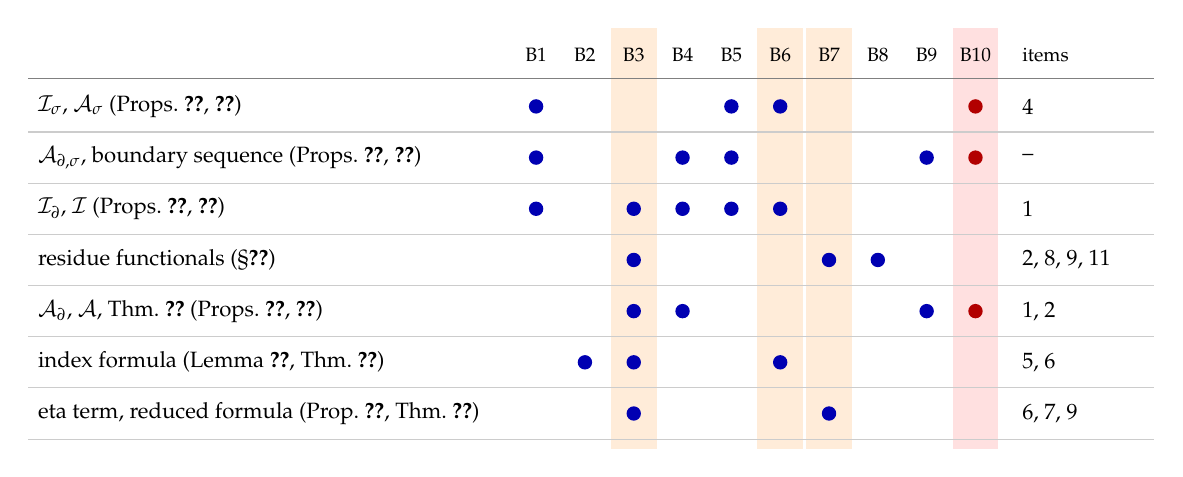
\begin{tikzpicture}[font=\footnotesize]
 \def\cx#1{\fpeval{6.45+0.62*(#1-1)}}
 \foreach \c in {3,6,7} \fill[orange!15] (\cx{\c}-0.29,0.35) rectangle (\cx{\c}+0.29,-5.0);
 \foreach \c in {10} \fill[red!12] (\cx{\c}-0.29,0.35) rectangle (\cx{\c}+0.29,-5.0);
 \foreach \i in {1,...,10} \node[font=\scriptsize,inner sep=0pt] at (\cx{\i},0) {B\i};
 \node[font=\scriptsize,anchor=west] at (12.5,0) {items};
 \draw[gray] (0,-0.3)--(14.3,-0.3);
 \foreach \r/\lab/\cols/\cor in {
   1/{\(\Is\), \(\As\) (Props.~\ref{prop:As}, \ref{prop:Is})}/{1,5,6,10}/{4},
   2/{\(\Ads\), boundary sequence (Props.~\ref{prop:Ads}, \ref{prop:boundaryLES})}/{1,4,5,9,10}/{--},
   3/{\(\Id\), \(\cI\) (Props.~\ref{prop:Id}, \ref{prop:I})}/{1,3,4,5,6}/{1},
   4/{residue functionals (\S\ref{sec:residues})}/{3,7,8}/{2, 8, 9, 11},
   5/{\(\Ad\), \(\cA\), Thm.~\ref{thm:main} (Props.~\ref{prop:Ad}, \ref{prop:HHA})}/{3,4,9,10}/{1, 2},
   6/{index formula (Lemma~\ref{lem:fedosov}, Thm.~\ref{thm:index})}/{2,3,6}/{5, 6},
   7/{eta term, reduced formula (Prop.~\ref{prop:eta}, Thm.~\ref{thm:reduced})}/{3,7}/{6, 7, 9}}{
   \node[anchor=west] at (0,-0.65*\r) {\lab};
   \foreach \c in \cols {
     \ifnum\c>9 \fill[red!70!black] (\cx{\c},-0.65*\r) circle (2.6pt);
     \else \fill[blue!70!black] (\cx{\c},-0.65*\r) circle (2.6pt);\fi}
   \node[anchor=west] at (12.5,-0.65*\r) {\cor};
   \draw[gray!40] (0,-0.65*\r-0.325)--(14.3,-0.65*\r-0.325);
 }
\end{tikzpicture}
\caption[Background facts and corrections used by the main results]{Which
main results use which background facts of
Section~\ref{subsec:background} (dots), and which items of the list in
Section~\ref{subsec:errata} concern them (last column). Blue dots: facts
proved in Appendices~\ref{cc:sec:cusp}--\ref{tr:sec}; on an orange column
the proof uses a step that is sketched or quoted ((B3): the calculus with
holomorphic parameters; (B6): Eilenberg--Zilber and Morita for H-unital
ideals with bundles; (B7): the inputs of the eta identification). The
red column is quoted: (B10), the last step of the convergence for
\(\As\) and \(\Ads\) when \(n\ge2\) (Remark~\ref{ha:rem:quoted}); for
\(n=1\) it is proved (Corollary~\ref{ha:cor:n1}). Everything built on the
homology of \(\As\) and \(\Ads\), including the corrected groups of
\(\cA\), rests on it when \(n\ge2\). The boundary connecting map (B9) is
proved (Theorem~\ref{ha:thm:bdry}); as a statement about the homology
groups it is used together with (B10). (The index formula uses the trace
computations of Section~\ref{sec:AdA}, not the homology groups.) Each row
also uses the rows above it, as in Figure~\ref{fig:roadmap}. Items 3 (not
used elsewhere), 10 (the foundations behind (B1)) and 12 (misprints) are
not shown. The row for \(\Id\) uses the convergence of its \(x\)-adic
spectral sequence, which is proved (Proposition~\ref{ha:prop:Idconv}),
modulo the sketched Lemma~\ref{ha:lem:mixed}(b).}
\label{fig:deps}
\end{figure}

\section{The closed case: Brylinski--Getzler and Wodzicki}\label{sec:closed}

Everything in \cite{MN} is modelled on the case \(\partial X=\varnothing\),
which MN recall in their introduction \cite[(1)--(5)]{MN}. We treat it
first, with proofs of the formulas that will be generalized later.

\subsection{The symbol algebra and its homology}
Let \(M\) be a closed manifold of dimension \(n\), let \(\Psi^{\Z}(M)\) be
the algebra of classical pseudodifferential operators of integral order,
and let \(\cA_M=\Psi^{\Z}(M)/\Psi^{-\infty}(M)\). A quantization identifies
\(\cA_M\) with formal sums \(\sum_{j\le m}a_j\) of smooth functions
\(a_j\) on \(T^*M\setminus0\), homogeneous of degree \(j\), with a star
product
\[
 a\star b=\sum_{l\ge0}P_l(a,b),\qquad P_0(a,b)=ab,\qquad
 P_1(a,b)-P_1(b,a)=-i\{a,b\},
\]
where \(P_l\) is bidifferential and lowers the total degree by \(l\).

\begin{theorem}[Brylinski--Getzler, Wodzicki \cite{BG,Wodzicki-cyclic}]
\label{thm:BG}
\(\HH_k(\cA_M)\cong H^{2n-k}(S^*M\times\Ssig)\), and dually
\(\HH^k(\cA_M)\cong H^k(S^*M\times\Ssig)\).
\end{theorem}

The proof is the model for Sections~\ref{sec:symbols}--\ref{sec:boundarysym}.
We give it in general form in Section~\ref{sec:hhtools}; see also
\cite[Ch.~10]{MelroseMicro}, whose argument we follow. In outline:
\begin{enumerate}
\item filter Hochschild chains by total order;
\item the associated graded algebra is commutative, so \(E^1\) is given
by homogeneous differential forms (HKR and Connes, (B5));
\item the first differential is the Poisson differential \(-i\delta\),
and the symplectic star operator turns it into the de Rham differential;
\item homogeneous forms of non-zero degree are exact, and forms of degree
\(0\) on \(T^*M\setminus0\cong S^*M\times(0,\infty)\) give
\(H^*(S^*M)\oplus H^{*-1}(S^*M)\,dr/r\), which is \(H^*(S^*M\times\Ssig)\);
\item the \(E^2\) term lies on one line, so the spectral sequence
degenerates and converges.
\end{enumerate}

\begin{question}
Where does the circle \(\Ssig\) come from, and why must one take operators
of \emph{all} integral orders?
\end{question}
\begin{answer}
The fibres of \(T^*M\setminus0\) are cones, \(S^{n-1}\times(0,\infty)_r\).
Homogeneous forms see the radial factor only through \(dr/r\), which is
invariant under dilation. So the homogeneous de Rham complex is that of
\(S^*M\times\Ssig\), where \(\Ssig=(0,\infty)/e^{\Z}\) is the quotient of
the radial half-line by integral dilations \cite[\S1]{MN}. The class
\(d\theta_\sigma=[dr/r]\) corresponds to \(i_{\lQ}\)
(Proposition~\ref{prop:Phi}). If only operators of order \(\le0\) were
allowed, the chains would not be closed under the shifts of order that
produce \(dr/r\). The homology is then infinite dimensional; see
\cite[\S15]{MN} and Section~\ref{subsec:other}. MN make the same point on
\cite[p.~3]{MN}.
\end{answer}

\subsection{The residue trace, the exterior derivation and the index}
Let \(Q\in\Psi^1(M)\) be positive, elliptic and invertible. For
\(A\in\Psi^m(M)\) the function \(\Tr(AQ^{-s})\) is holomorphic for
\(\operatorname{Re}s>m+n\) and extends meromorphically with simple poles.
Wodzicki's residue is \(\TrR(A)=\Res_{s=0}\Tr(AQ^{-s})\) \cite[(2)]{MN}.
It is a trace, independent of \(Q\), vanishes on \(\Psi^{-\infty}\), and
is given locally by (B8) (Theorem~\ref{tr:thm:res}):
\begin{equation}\label{eq:wodzicki}
 \TrR(A)=(2\pi)^{-n}\int_{S^*M}a_{-n}\,\nu,\qquad
 \nu=\iota_{R}\,\frac{\omega^n}{n!}\ \text{up to the orientation convention,}
\end{equation}
where \(R\) is the radial vector field. The \emph{regularized trace}
\(\widehat{\Tr}(A)\) is the constant term of \(\Tr(AQ^{-s})\) at \(s=0\).
The formula
\[
 D_{\lQ}(A)=[\lQ,A]=\frac{d}{ds}\Bigl(Q^sAQ^{-s}\Bigr)\Big|_{s=0}
\]
defines a derivation of \(\Psi^{\Z}(M)\), lowering order by one, which is
not inner \cite[\S6]{MN}.

\begin{lemma}[Trace defect]\label{lem:closeddefect}
For \(A,B\in\Psi^{\Z}(M)\),
\[
 \widehat{\Tr}([A,B])=\TrR(A[\lQ,B])=-\TrR([\lQ,A]B),\qquad
 \TrR([\lQ,C])=0 .
\]
\end{lemma}

\begin{proof}
For \(\operatorname{Re}s\) large, the trace property gives
\(\Tr([A,B]Q^{-s})=\Tr(A[B,Q^{-s}])\). Write
\[
 [B,Q^{-s}]=BQ^{-s}-Q^{-s}B=s\,M(s)Q^{-s},\qquad
 M(s)=\frac{B-Q^{-s}BQ^{s}}{s}.
\]
Then \(M\) is an entire family of fixed order with
\(M(0)=\frac{d}{ds}(-Q^{-s}BQ^s)|_{s=0}=[\lQ,B]\). Hence
\(\Tr([A,B]Q^{-s})=s\Tr(AM(s)Q^{-s})\). The function \(\Tr(AM(s)Q^{-s})\)
has at most a simple pole at \(s=0\), with residue \(\TrR(AM(0))\). So
the left side is regular at \(s=0\), with value \(\TrR(A[\lQ,B])\). For
the last identity take \(A=\mathrm{Id}\): the function
\(\Tr([\mathrm{Id},B]Q^{-s})\) vanishes identically, so
\(\TrR([\lQ,B])=0\). Applying this to \(C=AB\) gives
\(\TrR([\lQ,A]B)+\TrR(A[\lQ,B])=0\).
\end{proof}

\begin{proposition}[The index functional, MN (3)--(5)]\label{prop:closedindex}
The connecting map of \(0\to\Psi^{-\infty}\to\Psi^{\Z}\to\cA_M\to0\) sends
the trace to the Hochschild \(1\)-cocycle
\(\IF(A,B)=\TrR(A[\lQ,B])\) on \(\cA_M\). If \(A\in\Psi^m(M)\) is elliptic
with parametrix \(B\), then
\[
 \Ind(A)=\Tr([A,B])=\TrR\bigl(A[\lQ,A^{-1}]\bigr).
\]
\end{proposition}

\begin{proof}
The trace on \(\Psi^{-\infty}\) extends to the functional \(\widehat{\Tr}\)
on \(\Psi^{\Z}\). Its Hochschild coboundary \((b\widehat{\Tr})(A,B)=
\widehat{\Tr}([A,B])\) vanishes if \(A\) or \(B\) is smoothing, because
\(\TrR\) vanishes on \(\Psi^{-\infty}\). By Lemma~\ref{lem:closeddefect}
it equals \(\TrR(A[\lQ,B])\). Lemma~\ref{lem:conn} below then identifies
it with the image of \([\Tr]\) under the connecting map. For the index:
\(1-BA\) and \(1-AB\) are smoothing, \(\Ind A=\Tr(1-BA)-\Tr(1-AB)=
\Tr([A,B])\) (Fedosov), and \(\Tr([A,B])=\widehat{\Tr}([A,B])\) because
\([A,B]\) is smoothing.
\end{proof}

Since \(A[\lQ,A^{-1}]=-[\lQ,A]A^{-1}\), we also have
\[
 \Ind(A)=-\TrR\bigl([\lQ,A]A^{-1}\bigr)=-\TrR\bigl(A^{-1}[\lQ,A]\bigr).
\]
Keep this sign in mind; it is the source of
Correction~\ref{corr:ASsign}.

\subsection{Example: the circle}\label{subsec:circle}
Let \(M=S^1\), with modes \(e_k=e^{ik\theta}\), and let \(Q\) act by
\(Qe_k=\langle k\rangle e_k\), where \(\langle k\rangle=(1+k^2)^{1/2}\).

\emph{Homology.} \(S^*S^1=S^1\times\{\pm1\}\), so
\(S^*S^1\times\Ssig\) is two tori, and Theorem~\ref{thm:BG} gives
\[
 \dim\HH_k(\cA_{S^1})=2,\ 4,\ 2\qquad(k=0,1,2).
\]
In degree \(0\) there are \emph{two} independent residue traces,
\[
 \TrR^\pm(A)=\frac1{2\pi}\int_0^{2\pi}a_{-1}(\theta,\pm1)\,d\theta ,
\]
one for each direction of \(\xi\). Their sum is \(\TrR\). This is the
\(n=1\) phenomenon that will reappear at the boundary
(Correction~\ref{corr:n1}).

\emph{Index.} Let \(\Pi\) be the orthogonal projection onto
\(\operatorname{span}\{e_k:k\ge0\}\); it is a classical operator of order
\(0\). Put
\[
 A=e^{i\theta}\Pi+(1-\Pi),\qquad B=e^{-i\theta}\Pi+(1-\Pi).
\]
Then \(Ae_k=e_{k+1}\) for \(k\ge0\) and \(Ae_k=e_k\) for \(k<0\). So \(A\)
is injective and its range misses exactly \(e_0\), whence \(\Ind A=-1\).
A direct check gives \(BA=1\) and \(1-AB=R\), where \(R\) is the rank one
operator \(e_0\mapsto e_0-e_{-1}\). Therefore
\(\Tr([A,B])=-\Tr R=-1\), as Fedosov's formula requires. Now compute the
residue formula. For \(k\ge1\),
\[
 A[\lQ,B]e_k=A\bigl(\log\langle k-1\rangle-\log\langle k\rangle\bigr)e_{k-1}
 =\bigl(\log\langle k-1\rangle-\log\langle k\rangle\bigr)e_k
 =\Bigl(-\frac1k+O(k^{-2})\Bigr)e_k .
\]
For \(k\le-1\) the operator \(A[\lQ,B]\) vanishes on \(e_k\), and \(e_0\)
contributes a finite rank term. Hence
\[
 \TrR\bigl(A[\lQ,B]\bigr)=\Res_{s=0}\sum_{k\ge1}\Bigl(-\frac1k+O(k^{-2})
 \Bigr)\langle k\rangle^{-s}=-1=\Ind A .
\]
In symbol terms, \(A[\lQ,B]\) has \(a_{-1}(\theta,\xi)=-\xi^{-1}\) for
\(\xi>0\) and \(0\) for \(\xi<0\). Only \(\TrR^+\) contributes.
Figure~\ref{fig:circle} shows both computations.

\begin{figure}[htbp]
\centering
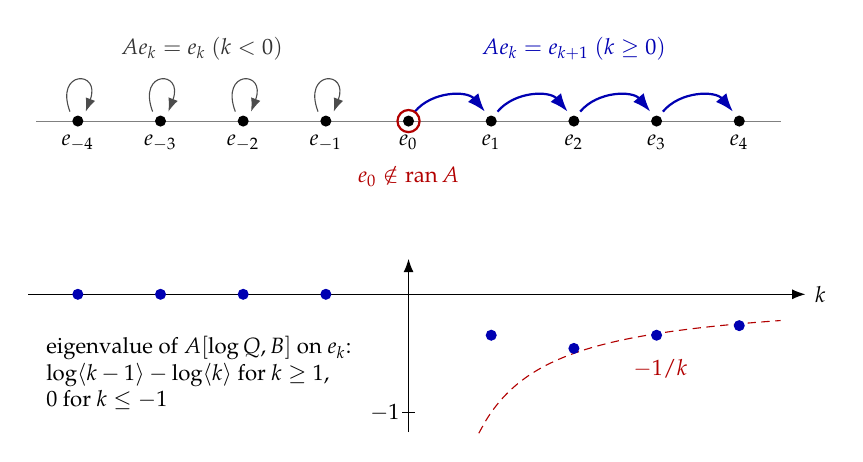
\begin{tikzpicture}[>=Latex,font=\footnotesize]
 \def\s{1.05}
 % top row: action of A on modes
 \draw[gray] (-4.5*\s,2.2)--(4.5*\s,2.2);
 \foreach \k in {-4,...,4}{\fill (\k*\s,2.2) circle (2pt);
   \node[below] at (\k*\s,2.15) {\(e_{\k}\)};}
 \foreach \k in {0,...,3} \draw[->,thick,blue!70!black] (\k*\s+0.08,2.32) to[bend left=50] (\k*\s+\s-0.08,2.32);
 \foreach \k in {-4,...,-1} \draw[->,gray!60!black] (\k*\s-0.1,2.32) .. controls (\k*\s-0.3,2.85) and (\k*\s+0.3,2.85) .. (\k*\s+0.1,2.32);
 \draw[red!70!black,thick] (0,2.2) circle (4pt);
 \node[blue!70!black,anchor=south] at (2*\s,2.85) {\(Ae_k=e_{k+1}\) \((k\ge0)\)};
 \node[gray!40!black,anchor=south] at (-2.5*\s,2.85) {\(Ae_k=e_k\) \((k<0)\)};
 \node[red!70!black,anchor=north,align=center] at (0,1.75) {\(e_0\notin\operatorname{ran}A\)};
 % bottom row: eigenvalues of A[log Q,B]
 \draw[->] (-4.6*\s,0)--(4.8*\s,0) node[right] {\(k\)};
 \draw[->] (0,-1.75)--(0,0.45);
 \draw (-0.08,-1.5)--(0.08,-1.5) node[left,xshift=-2pt] {\(-1\)};
 \draw[densely dashed,red!70!black,domain=0.85:4.5,samples=40,smooth]
   plot (\x*\s,{-1.5/\x});
 \foreach \k in {-4,...,-1} \fill[blue!70!black] (\k*\s,0) circle (2pt);
 \foreach \k in {1,...,4}{
   \pgfmathsetmacro{\v}{1.5*(ln(sqrt(1+(\k-1)^2))-ln(sqrt(1+\k^2)))}
   \fill[blue!70!black] (\k*\s,\v) circle (2pt);}
 \node[red!70!black,anchor=west] at (2.6*\s,-0.95) {\(-1/k\)};
 \node[anchor=west,align=left] at (-4.5*\s,-1.0)
   {eigenvalue of \(A[\lQ,B]\) on \(e_k\):\\ \(\log\langle k-1\rangle-\log\langle k\rangle\) for \(k\ge1\),\\ \(0\) for \(k\le-1\)};
\end{tikzpicture}
\caption[The Toeplitz-type operator on the circle]{The example of
Section~\ref{subsec:circle}, \(A=e^{i\theta}\Pi+(1-\Pi)\). Top: \(A\)
shifts the modes \(e_k\), \(k\ge0\), up by one and fixes the others, so
\(A\) is injective, its range misses \(e_0\), and \(\Ind A=-1\). Bottom:
\(A[\lQ,B]\) is diagonal on \(e_k\), \(k\ne0\), with eigenvalue
\(-1/k+O(k^{-2})\) for \(k\ge1\) and \(0\) for \(k\le-1\) (\(e_0\) gives
a finite rank term). The tail \(-1/k\) on one side only gives
\(\TrR(A[\lQ,B])=-1=\Ind A\): only \(\TrR^+\) contributes, and the
opposite order \(\TrR(A^{-1}[\lQ,A])\) gives \(+1\).}
\label{fig:circle}
\end{figure}

\begin{discussion}
The example fixes the sign convention for everything that follows:
\[
 \Ind A=\TrR\bigl(A[\lQ,A^{-1}]\bigr),\qquad\text{\emph{not}}\qquad
 \TrR\bigl(A^{-1}[\lQ,A]\bigr).
\]
The second expression equals \(+1\) here.
\end{discussion}

\section{The cusp calculus}\label{sec:cusp}

This section collects the facts about cusp operators that \cite{MN} uses.
It follows \cite[App.~A--C]{MN}, \cite{MazzeoMelrose} and
\cite{MelroseFibrations}. It is an informal tour: the proofs are in
Appendix~\ref{cc:sec:cusp}, which constructs the calculus directly on the
cylinder \(\R_t\times\partial X\) and does not use the triple space. We
begin with the half-line, where everything is explicit.

\subsection{Cusp structures and cusp vector fields}\label{subsec:cuspstructure}
A \emph{cusp structure} on \(X\) is a choice of boundary defining
function \(x\), modulo two kinds of change: multiplication by a positive
constant on each boundary component, and addition of a term in
\(x^2\CI(X)\) \cite[App.~A]{MN}. Equivalently, it is a trivialization of
the normal bundle of \(\partial X\), up to constant multiples on each
component. The \emph{cusp vector fields} are \cite[(6), (114)]{MN}
\[
 \mathcal V_c(X)=\{V\in\CI(X;TX):\ Vx\in x^2\CI(X)\}.
\]

\begin{lemma}[MN Lemma 20 and Corollary 4]\label{lem:cuspvf}
In coordinates \((x,y)\) near a boundary point, \(V\in\mathcal V_c(X)\)
if and only if \(V=a\,x^2\partial_x+\sum_jb_j\partial_{y_j}\) with
\(a,b_j\) smooth. If \(x'\) is another boundary defining function, then
\(\mathcal V_c\) is the same for \(x\) and \(x'\) exactly when \(x'\)
defines the same cusp structure.
\end{lemma}

\begin{proof}
Write \(V=\alpha\partial_x+\sum\beta_j\partial_{y_j}\). Then \(Vx=\alpha\),
so \(V\in\mathcal V_c\) if and only if \(\alpha=ax^2\). For the second
statement write \(x'=e^{f}x\), with \(f\) smooth. Then
\[
 (x^2\partial_x)x'=x^2e^f(1+x\partial_xf),\qquad
 \partial_{y_j}x'=x\,e^f\partial_{y_j}f .
\]
The first expression lies in \(x'^2\CI=x^2\CI\). The second lies in
\(x^2\CI\) if and only if \(\partial_yf=O(x)\) at \(\partial X\), that is,
if and only if \(f|_{\partial X}\) is locally constant. In that case
\(x'=cx+O(x^2)\) on each component, which is the stated equivalence.
\end{proof}

The cusp vector fields form a Lie algebra and a \(\CI(X)\)-module. Near the
boundary they are locally free on \(x^2\partial_x,\partial_{y_j}\). Hence
there is a vector bundle \({}^cTX\) with \(\mathcal V_c=\CI(X;{}^cTX)\).
Its dual is \(\cT\), with local frame \(dx/x^2,dy_j\). Over the interior
\({}^cTX=TX\), and globally \({}^cTX\cong TX\) as abstract bundles. So the
cosphere bundle \(Y=\Y=(\cT\setminus0)/\R^+\) is diffeomorphic to \(S^*X\).
Its boundary is \(Z=\Zb\), the sphere bundle of
\({}^cT^*_{\partial X}X=T^*\partial X\times\R_\tau\). If \(n\ge2\), each
component \(Z_j\) is an \(S^{n-1}\)-bundle over \(H_j\), hence connected.
If \(n=1\), each \(Z_j\) is the pair of points \(\tau=\pm1\).

MN also show that any two cusp structures are related by a diffeomorphism
isotopic to the identity \cite[Lemma~19]{MN}. So the algebras for
different structures are isomorphic. The proof integrates a vector field
transverse to the boundary that interpolates between the two defining
functions.

\subsection{The model: the half-line}\label{subsec:halfline}
Let \(X=[0,1)_x\). In the variable \(t=1/x\in(1,\infty)\), the cusp vector
field is \(x^2\partial_x=-\partial_t\) by \eqref{eq:t}. So the cusp
structure makes the end \(x\to0\) into a \emph{cylindrical end}
\(t\to\infty\) of a complete manifold. The dictionary:
\begin{center}
\renewcommand{\arraystretch}{1.25}
\begin{tabular}{ll}
 on \([0,1)_x\) & on \((1,\infty)_t\)\\\hline
 \(\CI([0,1))\) & smooth functions with expansions in powers of \(1/t\)\\
 \(\dCI([0,1))\) & functions rapidly decreasing as \(t\to\infty\)\\
 \(x^{-\Z}\CI([0,1))\) & functions with expansions \(\sum_{j\ge-p}c_jt^{-j}\)\\
 cusp density \(dx/x^2\) & \(dt\)\\
 exact cusp metric \(dx^2/x^4\) & \(dt^2\)\\
 \(\sum_ja_j(x)(x^2D_x)^j\) & \(\sum_ja_j(1/t)(-D_t)^j\)\\
 \(\In(P,\tau)\) & \(\sum_ja_j(0)\tau^j\)\\
\end{tabular}
\end{center}
\begin{figure}[htbp]
\centering
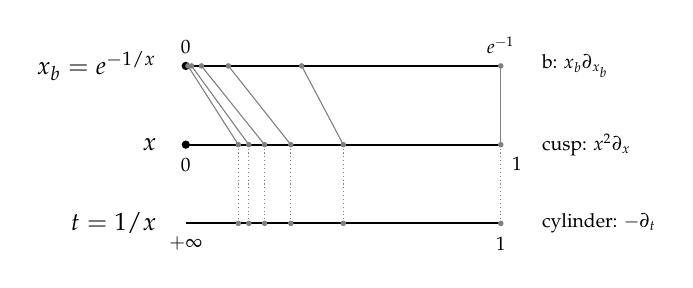
\begin{tikzpicture}[>=Latex]
 \foreach \y/\lab in {2/{x_b=e^{-1/x}},1/{x},0/{t=1/x}}{
   \draw[thick] (0,\y)--(4,\y);
   \node[left,font=\small] at (-0.25,\y) {\(\lab\)};
 }
 \fill (0,2) circle (1.5pt); \fill (0,1) circle (1.5pt);
 \node[above,font=\scriptsize] at (0,2.03) {\(0\)};
 \node[above,font=\scriptsize] at (4,2.03) {\(e^{-1}\)};
 \node[below,font=\scriptsize] at (0,0.95) {\(0\)};
 \node[anchor=north west,font=\scriptsize] at (4.02,0.97) {\(1\)};
 \node[below,font=\scriptsize] at (0,-0.05) {\(+\infty\)};
 \node[below,font=\scriptsize] at (4,-0.05) {\(1\)};
 \foreach \k in {1,2,3,4,5,6}{
   \pgfmathsetmacro{\px}{4/\k}
   \pgfmathsetmacro{\pb}{4*exp(1-\k)}
   \draw[gray] (\pb,2)--(\px,1);
   \draw[gray,densely dotted] (\px,1)--(\px,0);
   \fill[gray] (\pb,2) circle (1pt); \fill[gray] (\px,1) circle (1pt);
   \fill[gray] (\px,0) circle (1pt);
 }
 \node[right,font=\scriptsize] at (4.4,2) {b: \(x_b\partial_{x_b}\)};
 \node[right,font=\scriptsize] at (4.4,1) {cusp: \(x^2\partial_x\)};
 \node[right,font=\scriptsize] at (4.4,0) {cylinder: \(-\partial_t\)};
\end{tikzpicture}
\caption[The half-line in three coordinates]{The half-line in three
coordinates. The cusp vector field \(x^2\partial_x\) is \(-\partial_t\) in
\(t=1/x\), the generator of translations of a cylindrical end, and it is
the b-vector field \(x_b\partial_{x_b}\) in the transcendental coordinate
\(x_b=e^{-1/x}\) (Section~\ref{subsec:transcendental}). The gray marks
are the points \(t=1,2,\dots,6\): equally spaced in \(t\), at
\(x=1/t\), and at \(x_b=e^{-t}\), where they crowd exponentially towards
\(0\). All powers of \(x_b\) vanish to infinite order in \(x\).}
\label{fig:halfline}
\end{figure}

A cusp differential operator is thus a differential operator on the
half-line \((1,\infty)_t\) whose coefficients have expansions in \(1/t\).
Its indicial family is its ``value at \(t=\infty\)'', Fourier transformed
in \(t\). The pseudodifferential operators near the boundary are the
operators
\[
 Au(t)=\frac1{2\pi}\int\!\!\int e^{i(t-t')\xi}\,a\bigl(1/t,\xi\bigr)
 u(t')\,dt'\,d\xi,
\]
where \(a(x,\xi)\) is a classical symbol in \(\xi\), smooth in \(x\) up to
\(x=0\). The kernel is smooth off the diagonal and rapidly decreasing in
\(t-t'\) \cite[Props.~22, 23]{MN}. The translation invariant operators
(with \(a=a(\xi)\)) form the suspended algebra \(\Psis^{\Z}(\mathrm{pt})\),
the convolution operators by kernels that are classical conormal at
\(0\) and Schwartz at infinity. It is \emph{commutative}.

\begin{remark}[The compactification in \cite{MN}, (130)]\label{rem:SP}
MN identify \(\R\) with \((-1,1)\) via \(z\mapsto z/(1+z^2)^{1/2}\). Near
\(z=+\infty\) this gives \(1-z/\langle z\rangle=\frac12z^{-2}+O(z^{-4})\),
so the smooth structure it induces on \([-1,1]\) is that of \(\rho^2\)
with \(\rho=1/z\). In that structure \(\partial_z\) is not a cusp vector
field, and translations do not act smoothly. The identification
\cite[Prop.~22]{MN} and the description of \(\Psis\) on \cite[p.~44]{MN}
need the compactification by \(\rho=1/|z|\). For example one can use
\(z\mapsto\frac2\pi\arctan z\), for which \(1-\frac2\pi\arctan z=
\frac2\pi\arctan(1/z)\) is a smooth defining function in \(\rho\). Then
\(\partial_z=-\rho^2\partial_\rho\) is a cusp vector field, and the
translation \(z\mapsto z+c\) acts by \(\rho\mapsto\rho/(1+c\rho)\), which
is smooth. With this change the statements of \cite[App.~A]{MN} hold as
written.
\end{remark}

\begin{example}\label{ex:dt}
The operator \(P=x^2D_x+c\) on \([0,1)\) is \(-D_t+c\), and
\(\In(P,\tau)=\tau+c\). Its inverse on \(\R_t\), when \(c\notin\R\), is
convolution with an exponentially decreasing kernel. The indicial family is
invertible for all real \(\tau\) precisely when \(c\notin\R\). This is the
cusp version of ``no indicial roots on the real line''. There is no
condition off the real axis; compare Section~\ref{sec:comparison}.
\end{example}

\subsection{Kernels and the cusp double space}\label{subsec:double}
Globally, kernels are described on a blown-up double space
\cite[App.~A]{MN}. First blow up the corners \(H\times H\) of \(X^2\) to
obtain the b-double space \(X_b^2\), whose front face has the coordinate
\(s=x/x'\). The cusp structure picks out the point \(s=1\) on each fibre
of the b-front face, more precisely the fibre diagonal
\(\Phi_2(H)=\{s=1\}\times H^2\). Blowing these up gives
\[
 X_c^2=[X_b^2;\ \{\Phi_2(H)\}_H],\qquad
 \mu=\frac1x-\frac1{x'}=t-t' \quad\text{on the new front face }\mathrm{ff}_c .
\]
The interior of \(\mathrm{ff}_c\) is \(\R_\mu\times H^2\); see
Figure~\ref{fig:blowup}. The lifted diagonal meets the boundary of
\(X_c^2\) only in \(\mathrm{ff}_c\), at \(\mu=0\) \cite[Lemma~22]{MN}. Then
\(\Psic^m(X)\) consists of the kernels on \(X_c^2\) that are classical
conormal of order \(m\) at the lifted diagonal, smooth up to
\(\mathrm{ff}_c\), and rapidly vanishing at all other boundary faces
\cite[Def.~2]{MN}. In particular their restriction to \(\mathrm{ff}_c\) is
rapidly decreasing as \(|\mu|\to\infty\). The kernels in
\(\Psic^{-\infty}\) that vanish to infinite order also at \(\mathrm{ff}_c\)
are those of \(\cI\) \cite[Def.~1]{MN}. Proofs: Lemma~\ref{cc:lem:coords}
(coordinates on \(X_c^2\)), Proposition~\ref{cc:prop:MNdef} (agreement of
this description with the construction of Appendix~\ref{cc:sec:cusp}) and
Lemma~\ref{cc:lem:residual} (the ideal \(\cI\)). There kernels are
normalized by the right cusp density \(\nu_c\), equal to
\(x^{-2}dx\,\nu_\partial\) near \(\partial X\)
(Section~\ref{cc:subsec:conventions}); MN use half-densities
\cite[(118)]{MN}. Passing from one to the other multiplies the kernel by
\((\nu_c(z')/\nu_c(z))^{1/2}\). Near \(\mathrm{ff}_c\) this is
\(1-x\mu\) times a smooth positive function of \((y,y')\), and at the other
faces it grows at most polynomially, where the kernels vanish to infinite
order. So the two conventions define the same spaces of operators.

\emph{Cut-offs and pseudolocality.} We often multiply operators by
cut-off functions. Pseudolocality at the boundary, in the form
\(\phi A\psi\in\cI\) when \(\supp\phi\cap\supp\psi=\varnothing\), holds
only for cut-offs that are functions of \(x\) alone
(Lemma~\ref{cc:lem:local}(1)). If \(\phi\) and \(\psi\) depend on \(y\),
then \(\phi A\psi\) is smoothing but restricts to \(\mathrm{ff}_c\) as
\(\phi|_{\partial X}N(A)\psi|_{\partial X}\), which need not vanish, so it is
in \(\Psic^{-\infty}\) but not in \(\cI\). All the cut-offs used in the
main text to localize near or away from \(\partial X\) are functions of
\(x\).

\begin{figure}[htbp]
\centering
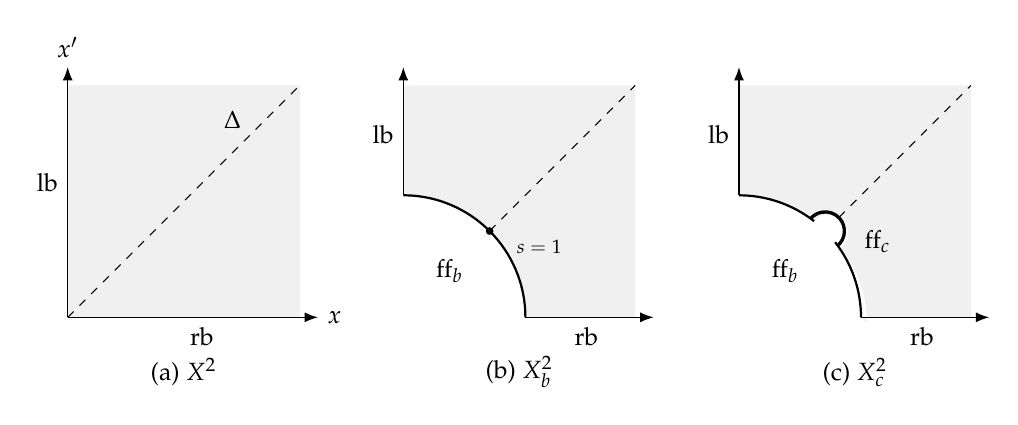
\begin{tikzpicture}[scale=1.55,>=Latex]
 % panel (a): X^2
 \begin{scope}
  \fill[gray!12] (0,0) rectangle (1.9,1.9);
  \draw[->] (0,0)--(2.05,0) node[right] {\small \(x\)};
  \draw[->] (0,0)--(0,2.05) node[above] {\small \(x'\)};
  \draw[dashed] (0,0)--(1.9,1.9);
  \node[font=\small] at (1.35,1.62) {\(\Delta\)};
  \node[font=\small,left] at (0,1.1) {lb};
  \node[font=\small,below] at (1.1,0) {rb};
  \node at (0.95,-0.45) {\small (a) \(X^2\)};
 \end{scope}
 % panel (b): X_b^2
 \begin{scope}[xshift=2.75cm]
  \fill[gray!12] (1,0)--(1.9,0)--(1.9,1.9)--(0,1.9)--(0,1) arc[start angle=90,end angle=0,radius=1];
  \draw[->] (1,0)--(2.05,0);
  \draw[->] (0,1)--(0,2.05);
  \draw[thick] (1,0) arc[start angle=0,end angle=90,radius=1];
  \draw[dashed] (0.7071,0.7071)--(1.9,1.9);
  \fill (0.7071,0.7071) circle (0.9pt);
  \node[font=\small] at (0.38,0.38) {\(\mathrm{ff}_b\)};
  \node[font=\scriptsize,anchor=west] at (0.85,0.58) {\(s=1\)};
  \node[font=\small,left] at (0,1.5) {lb};
  \node[font=\small,below] at (1.5,0) {rb};
  \node at (0.95,-0.45) {\small (b) \(X_b^2\)};
 \end{scope}
 % panel (c): X_c^2
 \begin{scope}[xshift=5.5cm]
  \fill[gray!12] (1,0)--(1.9,0)--(1.9,1.9)--(0,1.9)--(0,1)
   arc[start angle=90,end angle=52,radius=1]
   arc[start angle=139.4,end angle=-49.4,radius=0.157]
   arc[start angle=38,end angle=0,radius=1];
  \draw[->] (1,0)--(2.05,0);
  \draw[->] (0,1)--(0,2.05);
  \draw[thick] (1,0) arc[start angle=0,end angle=38,radius=1];
  \draw[thick] (0.6157,0.7880) arc[start angle=52,end angle=90,radius=1];
  \draw[very thick] (0.8090,0.5878) arc[start angle=-49.4,end angle=139.4,radius=0.157];
  \draw[dashed] (0.818,0.818)--(1.9,1.9);
  \node[font=\small] at (0.38,0.38) {\(\mathrm{ff}_b\)};
  \node[font=\small,anchor=west] at (0.95,0.62) {\(\mathrm{ff}_c\)};
  \node[font=\small,left] at (0,1.5) {lb};
  \node[font=\small,below] at (1.5,0) {rb};
  \node at (0.95,-0.45) {\small (c) \(X_c^2\)};
 \end{scope}
\end{tikzpicture}
\caption[The b- and cusp double spaces]{Near a corner \(H\times H\) of
\(X^2\) (suppressing \(H^2\)). (b) The b-blow-up replaces the corner by
the front face \(\mathrm{ff}_b\) with coordinate \(s=x/x'\); the diagonal
meets it at \(s=1\). (c) The cusp double space blows up the fibre diagonal
\(\{s=1\}\) once more. The new face \(\mathrm{ff}_c\) carries the coordinate
\(\mu=1/x-1/x'=t-t'\in[-\infty,\infty]\), the difference of the
suspension variables, and cusp kernels restrict to it as convolution kernels
in \(\mu\), rapidly decreasing at \(\mu=\pm\infty\). b-kernels are instead
smooth on \(\mathrm{ff}_b\) and convolution kernels in \(\log s\).}
\label{fig:blowup}
\end{figure}

\subsection{Symbols, quantization and the star product}\label{subsec:symbols}
The principal symbol gives exact sequences \cite[(11)]{MN}
\[
 0\to\Psic^{m-1}(X)\to\Psic^m(X)\xrightarrow{\sigma_m}
 \mathcal G^m(\cT)\to0,
\]
where \(\mathcal G^m(\cT)\) is the space of smooth functions on
\(\cT\setminus0\) that are homogeneous of degree \(m\). The symbol of a
product is the product of the symbols, and
\(\sigma_{m+m'-1}([A,B])=-i\{\sigma_m(A),\sigma_{m'}(B)\}\) with the
bracket \eqref{eq:poisson} (Proposition~\ref{cc:prop:symbol}). A global
quantization \(x^{-\Z}S^{\Z}(\cT)\to x^{-\Z}\Psic^{\Z}(X)\) exists
\cite[Prop.~24]{MN} (Proposition~\ref{cc:prop:quant}). It is linear, not
multiplicative. It induces the isomorphisms \eqref{eq:structure} for
\(\Is\) and \(\As\) \cite[(13)]{MN}, which are isomorphisms of vector
spaces, and transporting the product of \(\As\) through them gives a star
product
\[
 a\star b=\sum_{j\ge0}P_j(a,b),\qquad P_0(a,b)=ab,\qquad
 P_1(a,b)-P_1(b,a)=-i\{a,b\} \qquad\text{\cite[(137)--(138)]{MN}},
\]
with \(P_j\) bidifferential of total homogeneity \(-j\). In local
coordinates with the left quantization,
\(P_j(a,b)=\sum_{|\alpha|=j}(\alpha!)^{-1}\partial_\zeta^\alpha a\,
{}^cD^\alpha b\), where \(\zeta=(\tau,\eta)\) and \({}^cD=(x^2D_x,D_y)\)
up to lower order terms in the \(x\)-derivatives. Only \(P_0\) and the
antisymmetric part of \(P_1\) will matter.

\subsection{The indicial family, the suspended algebra and the twist}
\label{subsec:twist}
For a compact manifold \(H\) without boundary, \(\Psis^m(H)\) is the
algebra of pseudodifferential operators on \(\R_t\times H\) that are
invariant under translation in \(t\) and whose convolution kernels decrease
rapidly as \(|t|\to\infty\) \cite{MelroseEta}. Through \eqref{eq:Inkernel}
it is the same as the algebra of families \(\R\ni\tau\mapsto B(\tau)\in
\Psi^m(H)\) that are classical symbols jointly in \(\tau\) and in the
cotangent variables of \(H\). The smoothing part is
\(\Psis^{-\infty}(H)\cong\cS(\R)\widehat\otimes\Psi^{-\infty}(H)\). The
indicial map gives \cite[(12)]{MN}
\[
 0\to x\Psic^m(X)\to\Psic^m(X)\xrightarrow{\In}\Psis^m(\partial X)\to0 .
\]
More precisely, a choice of normal fibration identifies a collar with
\([0,\epsilon)\times\partial X\). The Taylor series \(\mathsf T\) of the
kernel at \(\mathrm{ff}_c\) then gives \cite[Prop.~25]{MN}
\begin{equation}\label{eq:taylor}
 \mathsf T:\ x^{-\Z}\Psic^{\Z}(X)/x^\infty\Psic^{\Z}(X)\ \cong\ \Psis^{\Z}(\partial X)\Lser{x},
 \qquad A\sim\sum_{j\ge-p}x^jA_{(j)} .
\end{equation}
Here \(\Psis^{\Z}(\partial X)\Lser{x}=\bigcup_m\Psis^m(\partial X)\Lser{x}\)
consists of the Laurent series \emph{whose coefficients have bounded
order}, the powers of \(x\) are written \emph{on the left}, and MN write
\(A_{-j}\) for our \(A_{(j)}\) \cite[(53)]{MN}. The product on the right
is not the naive one, because \(x\) does not commute with \(\Psis\); with
the twisted product of Proposition~\ref{cc:prop:taylor}, \(\mathsf T\) is
an algebra isomorphism (Proposition~\ref{cc:prop:taylor}; the exact
indicial sequence is Proposition~\ref{cc:prop:indicial}).

\begin{lemma}[The cusp twist]\label{lem:twist}
Let \(g\in\Psis^m(\partial X)\), acting on functions of \((t,y)\) with
\(t=1/x\) near the boundary. Write \(g'\) for the element with
\(\In(g',\tau)=\partial_\tau\In(g,\tau)\). Then:
\begin{enumerate}
\item \([t,g]=-i\,g'\);
\item \([x,g]=i\,xg'x=i\,x^2g'+O(x^3)\), and in particular
\([x,\partial_t]=x^2\);
\item \([\lx,g]=-\sum_{k\ge1}\frac1k\,x^k\,\mathrm{ad}_t^k(g)\), where
\(\mathrm{ad}_t^k(g)\) has indicial family \((-i\partial_\tau)^k\In(g)\).
\end{enumerate}
Parts (1) and (2) are also proved in Lemma~\ref{cc:lem:sus} and
Proposition~\ref{cc:prop:conj}.
The associated graded algebra of \(\Psis(\partial X)\Lser{x}\) for the
\(x\)-filtration is commutative modulo \(\Psi(\partial X)\). Its Poisson
bracket is \(\{x,\tau\}=-x^2\), that is, \(\{t,\tau\}=1\).
\end{lemma}

\begin{proof}
(1) follows from \eqref{eq:Inkernel}, since \([t,g]\) has kernel
\((t-t')\kappa(t-t')\). For (2),
\[
 [t^{-1},g]=t^{-1}g-gt^{-1}=-t^{-1}(tg-gt)t^{-1}=-t^{-1}[t,g]t^{-1}
 =i\,t^{-1}g't^{-1}.
\]
Moving the right-hand factor \(x\) past \(g'\) costs a further power of
\(x\), by the same identity. For \(g=\partial_t\) we have
\(\In(\partial_t,\tau)=-i\tau\), so \(g'=-i\) and \([x,\partial_t]=x^2\).
For (3), the kernel of \([\lx,g]=-[\log t,g]\) is
\(-(\log t-\log t')\kappa(t-t')\). With \(s=t-t'\),
\[
 \log t-\log t'=-\log\Bigl(1-\frac st\Bigr)=\sum_{k\ge1}\frac1k\,\frac{s^k}{t^k},
\]
and \(t^{-k}=x^k\) acts on the left. The kernel \(s^k\kappa(s)\) is that of
\(\mathrm{ad}_t^k(g)\), so its indicial family is
\((-i\partial_\tau)^k\In(g)\) by \eqref{eq:Inkernel}. The bracket of the
leading symbols follows from (2):
\(\sigma([x,\tau])=-i\{x,\tau\}\) and \([x,\tau]\) has leading term
\(ix^2\), so \(\{x,\tau\}=-x^2\). Then
\(\{t,\tau\}=-x^{-2}\{x,\tau\}=1\).
\end{proof}

\begin{discussion}
\textbf{What the twist means.} In \(\Id\) and \(\Ad\) the ``Laurent
variable'' \(x\) is the function \(1/t\) on the suspension line, and the
coefficients are functions of \(D_t\). So these algebras are
quantizations of functions of \((t,\tau)\) near \(t=+\infty\), and \(t\)
and \(\tau\) are canonically conjugate. In a Laurent series in \(x\), a
derivative in \(\tau\) costs one power of \(x\). This is why the
associated graded algebra is commutative and why the first differential
of the \(x\)-adic spectral sequence is a Poisson differential, exactly as
for the order filtration (Section~\ref{sec:indicial}). In the b-calculus
the corresponding relation is \(x^{-1}Ax=\alpha(A)\), where \(\alpha\) is
the complex shift \(\lambda\mapsto\lambda-i\). This automorphism does
\emph{not} become trivial on the associated graded algebra; see
Section~\ref{sec:comparison}. Figure~\ref{fig:twist} contrasts the two.
\end{discussion}

\begin{figure}[htbp]
\centering
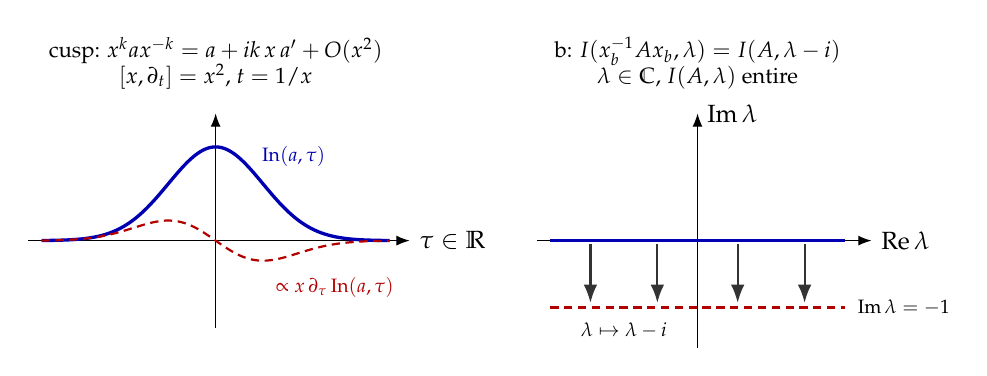
\begin{tikzpicture}[>=Latex,scale=0.85]
 \begin{scope}
  \draw[->] (-2.8,0)--(2.9,0) node[right] {\small \(\tau\in\R\)};
  \draw[->] (0,-1.3)--(0,1.9);
  \draw[very thick,blue!70!black,domain=-2.6:2.6,samples=80,smooth]
    plot (\x,{1.4*exp(-\x*\x)});
  \draw[thick,densely dashed,red!70!black,domain=-2.6:2.6,samples=80,smooth]
    plot (\x,{-0.5*\x*1.4*exp(-\x*\x)});
  \node[font=\scriptsize,blue!70!black,anchor=west] at (0.55,1.25) {\(\In(a,\tau)\)};
  \node[font=\scriptsize,red!70!black,anchor=north west] at (0.75,-0.4)
    {\(\propto x\,\partial_\tau\In(a,\tau)\)};
  \node[font=\footnotesize,align=center] at (0,2.65)
    {cusp: \(x^kax^{-k}=a+ik\,x\,a'+O(x^2)\)\\ \([x,\partial_t]=x^2\), \(t=1/x\)};
 \end{scope}
 \begin{scope}[xshift=7.2cm]
  \draw[->] (-2.4,0)--(2.6,0) node[right] {\small \(\operatorname{Re}\lambda\)};
  \draw[->] (0,-1.6)--(0,1.9) node[right] {\small \(\operatorname{Im}\lambda\)};
  \draw[very thick,blue!70!black] (-2.2,0)--(2.2,0);
  \draw[very thick,red!70!black,densely dashed] (-2.2,-1)--(2.2,-1);
  \foreach \a in {-1.6,-0.6,0.6,1.6} \draw[->,thick,gray!40!black] (\a,-0.05)--(\a,-0.93);
  \node[font=\scriptsize,anchor=west] at (2.25,-1) {\(\operatorname{Im}\lambda=-1\)};
  \node[font=\scriptsize,anchor=north] at (-1.1,-1.08) {\(\lambda\mapsto\lambda-i\)};
  \node[font=\footnotesize,align=center] at (0,2.65)
    {b: \(I(x_b^{-1}Ax_b,\lambda)=I(A,\lambda-i)\)\\ \(\lambda\in\C\), \(I(A,\lambda)\) entire};
 \end{scope}
\end{tikzpicture}
\caption[The cusp twist versus the b-twist]{Conjugation by powers of
\(x\). Left, the cusp case (Lemmas~\ref{lem:twist}
and~\ref{lem:commutators}): for \(a\) of \(x\)-degree zero,
\(x^kax^{-k}=a+ik\,x\,a'+O(x^2)\), where \(a'\) has indicial family
\(\partial_\tau\In(a,\tau)\). The correction (dashed) is a derivative in
\(\tau\) and costs one power of \(x\), so it disappears in the associated
graded algebra, which is commutative with Poisson bracket
\(\{t,\tau\}=1\). Right, the b-case: conjugation by \(x_b\) evaluates the
indicial family on the line \(\operatorname{Im}\lambda=-1\). This is a
finite shift, an automorphism that survives in the associated graded
algebra (Section~\ref{sec:comparison}).}
\label{fig:twist}
\end{figure}

\subsection{The transcendental blow-up and the b-calculus}
\label{subsec:transcendental}
The b-vector fields are spanned by \(x_b\partial_{x_b}\) and
\(\partial_y\). Put \cite[(143)]{MN}
\[
 x_b=e^{-1/x},\qquad\text{so that}\qquad
 \frac{dx_b}{dx}=\frac{x_b}{x^2},\qquad
 x_b\partial_{x_b}=x^2\partial_x .
\]
Thus b-differential operators in \((x_b,y)\) pull back to cusp
differential operators in \((x,y)\). A change \(x_b'=a(y)x_b+O(x_b^2)\)
of the b-defining function changes \(x\) to
\(x'=x/(1-x\log a)+O(x^\infty)=x+x^2\log a+O(x^3)\). If \(a\) is constant
on each component, this is the same cusp structure. In general the two
structures are related by Lemma~\ref{lem:cuspvf} up to the isotopy of
\cite[Lemma~19]{MN}. MN quote that b-pseudodifferential operators lift
to cusp operators and that the lifts are dense \cite[Prop.~26]{MN}. The
first statement is Proposition~\ref{cc:prop:transcendental}; the density
is not proved here and not used (Remark~\ref{cc:rem:density}).

Two features of the lift explain why it is useful.
\begin{enumerate}
\item The b-indicial family \(I(A,\lambda)\) of \cite{Notes} becomes
the cusp indicial family with \(\tau=\lambda\in\R\)
(Section~\ref{subsec:indicialvariable}).
\item A b-operator is \(A_0+x_bA_1+\dots\), with \(A_0\) dilation
invariant. After the lift, \(A_0\) is translation invariant in \(t\), and
\(x_b=e^{-1/x}\) vanishes to infinite order in \(x\). So the Laurent
series \eqref{eq:taylor} of a lifted b-operator is just \(\In(A)\), with
no higher terms.
\end{enumerate}
A b-operator whose indicial family is invertible on \(\R\) (that is, Fredholm
on \(L^2_b\)) therefore lifts to a fully elliptic cusp operator. The cusp
index formula applies to it, and its eta term is the b-eta invariant of
the indicial family, up to the local correction \(\delta_Q\) of
Proposition~\ref{prop:eta}. The b-Laurent algebra \(x_b^{-\Z}\Psi_b^{\Z}\) would
require invertibility for \emph{all} \(\lambda\in\C\)
(Section~\ref{sec:comparison}). This is the ``problem with completeness''
mentioned in \cite[p.~3]{MN}. Note also that Laurent series in \(x_b\) and
Laurent series in \(x=1/\log(1/x_b)\) are different algebras, so the lift
does not identify the two Hochschild computations \cite{HHb}.

\begin{question}
Why does the cusp calculus avoid the completeness problem, if the two
calculi have isomorphic norm closures \cite[p.~3]{MN}?
\end{question}
\begin{answer}
The norm closures see only the boundary behaviour on the real line. The
\(\CI\) algebras used for Hochschild homology see more. In the small
b-calculus, indicial families are \emph{entire} functions of
\(\lambda\in\C\). Inverting an operator modulo \(x_b^\infty\Psi_b^{-\infty}\)
means inverting its Taylor series at \(\mathrm{ff}_b\), so the inverse of
the indicial family must again be entire. Hence \(I(A,\lambda)\) must be
invertible for \emph{every} \(\lambda\in\C\) \cite[Lemma
``invertible'']{HHb}. Dirac operators never satisfy this. In the cusp
calculus conjugation by \(x\) acts through the twist of
Lemma~\ref{lem:twist}, which only adds terms of higher order in \(x\). So
only invertibility on \(\R\) is needed.
\end{answer}

\subsection{Ellipticity, cusp metrics and complex powers}
\label{subsec:elliptic}
An element of \(x^{-p}\Psic^m(X)\) is \emph{elliptic} if its principal
symbol (after removing \(x^{-p}\)) is invertible on \(\cT\setminus0\). It
is \emph{fully elliptic} if, in addition, its leading indicial family is
invertible for all real \(\tau\). In the Laurent setting this is
invertibility in \(\cA\) with matched orders: \(A\in x^{-p}\Psic^m(X)\) is
fully elliptic if and only if there is \(B\in x^p\Psic^{-m}(X)\) with
\(AB-1,BA-1\in\cI\) (Theorem~\ref{cc:thm:parametrix}, (B2)).

\begin{remark}[Exact cusp metrics]\label{rem:cuspmetric}
\cite[App.~B]{MN} writes an exact cusp metric as \(dx^2/x^4+h/x^2\). The
orthonormal frames of that metric are spanned by \(x^2\partial_x\) and
\(x\partial_y\), which are the \emph{scattering} vector fields. Its
Laplacian is a cusp differential operator, but its cusp symbol
\(\tau^2+x^2|\eta|^2\) degenerates at \(x=0\). So it is not cusp-elliptic,
and \((\Delta+1)^{-s/2}\) is not a cusp family of order \(-s\). The metric
compatible with \(\mathcal V_c\) is
\[
 g=\frac{dx^2}{x^4}+h=dt^2+h\quad\text{near }\partial X ,
\]
a metric with cylindrical ends. Its Laplacian has cusp symbol
\(\tau^2+|\eta|_h^2\). This is the metric to use in \cite[\S5]{MN}.
\end{remark}

For a positive invertible elliptic \(Q\in\Psic^1(X)\), such as
\((\Delta_g+1)^{1/2}\) for the metric of Remark~\ref{rem:cuspmetric}, the
complex powers \(Q^{-s}\) form an entire family of order \(-s\) (B3).
Appendix~\ref{tr:sec} avoids the spectral theory of \(Q\): any admissible
family \(Q(s)\) of order \(-s\) with \(Q(0)=\mathrm{Id}\) can be used
(Proposition~\ref{tr:prop:Q}, Definition~\ref{tr:def:cuspfam}). The
formal logarithm
\[
 \lQ=\frac{d}{ds}Q^s\Big|_{s=0}
\]
is not in the calculus, but commutators with it are. If \(Q\) is
asymptotically translation invariant, \(\In(Q)=Q_0=(D_t^2+\Delta_{\partial
X}+1)^{1/2}\), and this \(Q_0\) is the regularizer used in \cite[(60)]{MN}.

\section{The Hochschild homology toolkit}\label{sec:hhtools}

This section collects the homological algebra used in \cite{MN}, in the form
in which we use it. Several statements are adapted from the companion notes
\cite{HHb} and from \cite[Ch.~10]{MelroseMicro}; we say so in each case.

\subsection{Chains of topological algebras}\label{subsec:chains}
For a Fr\'echet algebra \(\mathfrak A\), the space of \(k\)-chains is the
completed projective tensor product \(C_k(\mathfrak A)=\mathfrak
A^{\widehat\otimes(k+1)}\) \cite[(36)]{MN}. Most of our algebras are
increasing unions \(\mathfrak A=\bigcup_N\mathfrak A_N\) of nuclear
Fr\'echet spaces with \(\mathfrak A_N\mathfrak A_M\subset\mathfrak
A_{N+M}\); for example \(\mathfrak A_N=x^{-N}\Psic^N(X)\). For these we
take
\[
 C_k(\mathfrak A)=\varinjlim_N\mathfrak A_N^{\widehat\otimes(k+1)} .
\]
Ideals and quotients carry the induced filtrations \cite[\S``The chain
model'']{HHb}. The basic examples are
\[
 \CI(M)^{\widehat\otimes(k+1)}=\CI(M^{k+1}),\qquad
 \dCI(M)^{\widehat\otimes(k+1)}=\dCI(M^{k+1})
\]
for compact manifolds with boundary \cite[proof of Lemma~1]{MN}. Here
\(\dCI(M^{k+1})\) denotes functions vanishing to infinite order at all
boundary faces of the manifold with corners \(M^{k+1}\). Since nuclear
completed tensor products preserve short exact sequences of Fr\'echet
spaces \cite{Treves}, for a closed ideal \(J\subset\mathfrak A\) the
sequence
\begin{equation}\label{eq:chainses}
 0\to\cK_\bullet\to C_\bullet(\mathfrak A)\to C_\bullet(\mathfrak A/J)\to0
\end{equation}
is exact. Here \(\cK_k\) is the closed span of the chains with at least one
entry in \(J\) \cite[Lemma ``Exactness of chain spaces'']{HHb}; see
Lemma~\ref{ha:lem:exact} for a proof that needs no continuous section of
\(\mathfrak A\to\mathfrak A/J\).

\subsection{H-unitality and excision}\label{subsec:excision}
An algebra \(J\) is \emph{H-unital} if its bar complex \((C_\bullet(J),b')\)
is acyclic \cite{Wodzicki}. It is \emph{topologically} H-unital if there is
a continuous contraction \(E\) with \(b'E+Eb'=1\). A unital algebra is
H-unital, with \(E(a_0\otimes\dots\otimes a_k)=1\otimes a_0\otimes\dots
\otimes a_k\).

\begin{background}[Wodzicki's excision theorem, (B4); proved in Theorem~\ref{ha:thm:excision}]\label{bg:excision}
If \(J\subset\mathfrak A\) is a closed ideal that is topologically
H-unital, then \(C_\bullet(J)\to\cK_\bullet\) is a quasi-isomorphism. Hence
\eqref{eq:chainses} gives a long exact sequence
\[
 \cdots\to\HH_k(J)\to\HH_k(\mathfrak A)\to\HH_k(\mathfrak A/J)
 \xrightarrow{\partial}\HH_{k-1}(J)\to\cdots .
\]
To compute \(\partial[c]\), lift the cycle \(c\) to a chain \(\tilde c\) of
\(\mathfrak A\). Then \(b\tilde c\in\cK\), and \(\partial[c]\) is its
class.
\end{background}

The proof, by filtering \(\cK\) by the position of the entries from \(J\)
and contracting the graded pieces with the bar contraction of \(J\), is
Theorem~\ref{ha:thm:excision}; Example~\ref{ha:ex:noexcision} shows what
goes wrong without H-unitality. The topological version needs the
contraction to be continuous, and this is what Lemma~\ref{lem:Hunital}
provides.

\begin{lemma}[Connecting maps on cocycles]\label{lem:conn}
Under the hypotheses of \ref{bg:excision}, let \(\varphi\) be a
\((k-1)\)-cocycle on \(J\). Let \(\hat\varphi\) be a continuous
\((k-1)\)-cochain on \(\mathfrak A\) that extends \(\varphi\) and such that
\(b\hat\varphi\) vanishes whenever one of its arguments lies in \(J\). Then
\(b\hat\varphi\) descends to a \(k\)-cocycle on \(\mathfrak A/J\) that
represents \(\partial^*[\varphi]\); that is,
\(\langle\varphi,\partial[c]\rangle=\langle b\hat\varphi,c\rangle\).
\end{lemma}

\begin{proof}
This is \cite[Lemma ``Connecting maps on cocycles'']{HHb}. The cochain
\(\hat\varphi\) restricted to \(\cK\) is a cocycle there, because
\(b\hat\varphi\) vanishes on \(\cK\). It restricts to \(\varphi\) on
\(C(J)\), so it represents \([\varphi]\) under the quasi-isomorphism. Hence
\(\langle\varphi,\partial[c]\rangle=\langle\hat\varphi,b\tilde c\rangle=
\langle b\hat\varphi,\tilde c\rangle\), and the last pairing depends only on
the image \(c\) of \(\tilde c\).
\end{proof}

This lemma is how every boundary map in \cite{MN} is computed: extend a
trace from an ideal by analytic continuation, and compute the coboundary of
the extension. MN's formula (17) is the case of the traces on \(\Is\) and
\(\Id\).

\subsection{Derivations}\label{subsec:derivations}

\begin{lemma}[MN \S6]\label{lem:iD}
Let \(D\) be a derivation of \(\mathfrak A\) and
\(i_D(a_0\otimes a_1\otimes\dots\otimes a_k)=a_0D(a_1)\otimes a_2\otimes
\dots\otimes a_k\). Then \(bi_D+i_Db=0\). If \(D=[h,\cdot\,]\) with
\(h\in\mathfrak A\) (\(\mathfrak A\) unital), then
\[
 i_D=bR_h-R_hb,\qquad R_h(a_0\otimes\dots\otimes a_k)=a_0h\otimes a_1
 \otimes\dots\otimes a_k .
\]
So \(i_D\) induces a map \(\HH_k\to\HH_{k-1}\) that vanishes for inner
derivations. Dually, \(b(i_D\varphi)=-i_D(b\varphi)\) for cochains.
\end{lemma}

\begin{proof}
Both identities are checked on elementary tensors. We do \(k=2\); the
general case is the same bookkeeping. On the one hand,
\[
 i_Db(a_0\otimes a_1\otimes a_2)=a_0a_1D(a_2)-a_0D(a_1a_2)+a_2a_0D(a_1)
 =-a_0D(a_1)a_2+a_2a_0D(a_1),
\]
while \(bi_D(a_0\otimes a_1\otimes a_2)=b(a_0D(a_1)\otimes a_2)=
a_0D(a_1)a_2-a_2a_0D(a_1)\). The sum vanishes. For the inner case,
\[
 bR_h(a_0\otimes a_1\otimes a_2)-R_hb(a_0\otimes a_1\otimes a_2)
 =a_0ha_1\otimes a_2-a_0a_1h\otimes a_2=a_0[h,a_1]\otimes a_2 ,
\]
since the terms \(a_0h\otimes a_1a_2\) and \(a_2a_0h\otimes a_1\) occur in
both \(bR_h\) and \(R_hb\) and cancel.
\end{proof}

In \cite{MN} the derivations \(D_{\lQ}\) and \(D_{\lx}\) are commutators
with elements \emph{not} in the algebra \cite[(63)--(64)]{MN}. Changing
\(Q\) or \(x\) changes them by commutators with
\(\log(Q'/Q)\in\Psic^0(X)\) or \(\log(x'/x)\in\CI(X)\), which are inner.
So the maps \(i_{\lQ}\) and \(i_{\lx}\) on homology do not depend on the
choices. The ideals \(\Is\), \(\Id\), \(\cI\) are preserved by both
derivations, and \(R_h\) maps chains of an ideal to chains of the same
ideal. So the same independence holds for the ideals.

\subsection{Explicit H-unitality contractions}\label{subsec:Hunital}

\begin{lemma}\label{lem:Hunital}
Let \(V,W\) be nuclear Fr\'echet spaces with a continuous pairing
\(\langle\cdot,\cdot\rangle:W\times V\to\C\). Let \(\mathcal K=V\widehat
\otimes W\) be the algebra with product \((v\otimes w)(v'\otimes w')=\langle
w,v'\rangle v\otimes w'\), and fix \(\psi\in W\), \(\tilde\psi\in V\) with
\(\langle\psi,\tilde\psi\rangle=1\). Then
\[
 E\bigl((v\otimes w)\otimes c\bigr)=(v\otimes\psi)\otimes(\tilde\psi\otimes
 w)\otimes c
\]
is a continuous contraction of the bar complex. Hence the algebras
\[
 \Psi^{-\infty}(H)=\CI(H)\widehat\otimes\CI(H),\qquad
 \cI=\dCI(X)\widehat\otimes\dCI(X)
\]
are topologically H-unital.
Moreover \(\HH_0(\mathcal K)\cong\C\), spanned by the trace
\(v\otimes w\mapsto\langle w,v\rangle\), and \(\HH_k(\mathcal K)=0\) for
\(k>0\).
\end{lemma}

\begin{proof}
The contraction is \cite[Lemma ``Explicit contractions'']{HHb}:
\(d_0E=1\) because \((v\otimes\psi)(\tilde\psi\otimes w)=v\otimes w\), and
\(d_{i+1}E=Ed_i\) for \(i\ge0\), so \(b'E+Eb'=1\). The homology statement is
Morita invariance for the smoothing kernels
(Lemma~\ref{ha:lem:morita}, adapted from \cite[Lemma ``Morita invariance
for smoothing kernels'']{HHb}), applied with \(\mathfrak A=\C\).
\end{proof}

\subsection{The Hochschild--Kostant--Rosenberg map and Connes' theorem}
\label{subsec:HKR}
For a commutative algebra the map \cite[after (26)]{MN}
\[
 \chi(f_0\otimes f_1\otimes\dots\otimes f_k)=\frac1{k!}\,f_0\,df_1\wedge
 \dots\wedge df_k
\]
satisfies \(\chi\circ b=0\). Conversely the antisymmetrization
\(\varphi(f_0;f_1,\dots,f_k)=\sum_{\sigma\in\mathfrak S_k}\sgn(\sigma)f_0
\otimes f_{\sigma(1)}\otimes\dots\otimes f_{\sigma(k)}\) is a cycle with
\(\chi\varphi(f_0;f_1,\dots,f_k)=f_0\,df_1\wedge\dots\wedge df_k\).

\begin{background}[Connes' theorem, (B5); proved in Theorems~\ref{ha:thm:connes} and~\ref{ha:thm:variants}]\label{bg:connes}
For a compact manifold \(M\), possibly with boundary or corners, \(\chi\)
induces isomorphisms \(\HH_k(\CI(M))\cong\CI(M;\Lambda^k)\) and
\(\HH_k(\dCI(M))\cong\dCI(M;\Lambda^k)\). The same holds, fibrewise, for
smooth functions on a manifold with values in a commutative nuclear
algebra of Laurent or formal series.
\end{background}

The proof for compact manifolds with corners, adapted from
\cite[Ch.~10]{MelroseMicro}, is Theorem~\ref{ha:thm:connes}. The formal,
Laurent, flat and Schwartz versions are Theorem~\ref{ha:thm:variants}, and
the version for homogeneous functions on a cone bundle, which is what the
symbol algebras need, is Corollary~\ref{ha:cor:homog}.

\subsection{Filtered complexes and the convergence of spectral sequences}
\label{subsec:convergence}
Let \(C_k=\{\sum_{p\le P}c_p:\ c_p\in C_{p,k}\}\) be a complex of formal
sums, bounded above in \(p\), with differential \(b=\sum_{l\ge0}b_l\),
where \(b_l:C_{p,k}\to C_{p-l,k-1}\). The filtration \(F_p=\{c:\ c_q=0\
\text{for}\ q>p\}\) is exhaustive and separated, and we assume it is
complete. (This assumption is not automatic: the chain model of
Section~\ref{subsec:chains} is \emph{not} complete for the order
filtration, and completeness is restored by passing to the mixed complexes
of Lemma~\ref{ha:lem:mixed}; see Remark~\ref{rem:poles}.) Put
\(E^1_{p,k}=H_k(C_{p,\bullet},b_0)\). Then \(b_1\) induces
\(d^1:E^1_{p,k}\to E^1_{p-1,k-1}\), and we write \(E^2=H(E^1,d^1)\).

\begin{proposition}[Degeneration and convergence {\cite[Prop.~``convergence'']{MelroseMicro}}]
\label{prop:convergence}
Suppose there is an integer \(n\) such that \(E^2_{p,k}=0\) whenever
\(p\ne k-n\). Then every class in \(H_k(C,b)\) has a representative in
\(F_{k-n}C_k\), and
\[
 \Theta:H_k(C,b)\to E^2_{k-n,k},\qquad[c]\mapsto[c_{k-n}],
\]
is an isomorphism. All differentials \(d^r\), \(r\ge2\), vanish.
\end{proposition}

\begin{proof}
This is Proposition~\ref{ha:prop:algconv}, where the proof is given in
full. The key step lowers the order of a cycle whose leading term has
vanishing \(E^2\)-class by subtracting \(b(x+y)\), with \(x\) a
\(b_0\)-cycle one order up and \(y\) a correction at the same order;
completeness is used to sum the resulting series of corrections, and the
higher differentials vanish because they leave the line \(p=k-n\).
\end{proof}

\begin{remark}[Completeness and pole orders]\label{rem:poles}
Proposition~\ref{prop:convergence} needs a complete filtration, and the
chain model of Section~\ref{subsec:chains} is not complete: a series such
as \(\sum_jr^j\otimes r^{-2j}\) has total orders tending to \(-\infty\)
but lies in no single \(\mathfrak A_N^{\widehat\otimes2}\)
(Appendix~\ref{ha:sec}, after Proposition~\ref{ha:prop:algconv}). The
remedy, taken from \cite[\S``Convergence and degeneration'']{HHb}, is to
compute with the mixed complexes \(C(\mathfrak B,\mathfrak A)\) of
Lemma~\ref{ha:lem:mixed}, whose stages are complete and which compute
\(\HH(\mathfrak A)\). For the closed symbol algebra and for \(\Is\) this
gives convergence (Theorem~\ref{ha:thm:conv}).

For the algebras with Laurent singularities at the boundary (\(\As\) and
\(\Ads\)) one also needs the corrections in the proof to stay in a fixed
pole stage. MN say convergence ``follows directly, as in the boundaryless
case'' \cite[p.~12]{MN}. In the b-calculus this is proved in
\cite[\S``Convergence and degeneration'']{HHb}, using the invertibility of
\(\mathcal L_{x\partial_x}\) on leading coefficients. That argument does
\emph{not} apply with the cusp Poisson structure: the cusp Lie derivative
\(\mathcal L_{x^2\partial_x}\) raises the power of \(x\), so it is nilpotent
on leading coefficients, and a cycle such as \(x^{-L}|\tau|^p\) has no
primitive in its own stage although it is exact in the direct limit
(Example~\ref{ha:ex:obstruction}). What survives is
Proposition~\ref{ha:prop:laurent}: representatives on the critical line
exist, \(\Theta\) is well defined, and the corrections can be found if
the pole bound is allowed to grow by two at each order. Convergence for
\(\As\) and convergence for \(\Ads\) are equivalent
(Proposition~\ref{ha:prop:equiv}). For \(n=1\) both hold: the
\(x\)-adic filtration of \(\Ads\), in stages with a margin of two poles,
proves it (Proposition~\ref{ha:prop:xadic}, Corollary~\ref{ha:cor:n1}).
For \(n\ge2\) the remaining step, a uniform pole bound, is quoted from
\cite[p.~12]{MN} (Remark~\ref{ha:rem:quoted}); it is item (B10) of
Section~\ref{subsec:background}. In what follows, for \(n\ge2\),
\emph{convergence for \(\As\) and \(\Ads\) is to be read as resting on
(B10)}. For \(\Is\) (rapid vanishing at the boundary) and for the closed
case no issue arises.
\end{remark}

\subsection{The Poisson differential and the symplectic star}
\label{subsec:poissonstar}
Let \(V\to M\) be a real vector bundle with a symplectic structure on
\(V\setminus0\) that is homogeneous of degree \(1\) under dilations. The
examples are \(T^*M\) and \(\cT\) with the forms of
Section~\ref{subsec:coords}. Let \(\Pi\) be the Poisson bivector and
\(\iota_\Pi\) contraction with it. The Koszul--Brylinski differential is
\(\delta=\iota_\Pi d-d\iota_\Pi\), which maps \(k\)-forms of homogeneity
\(p\) to \((k-1)\)-forms of homogeneity \(p-1\). On functions,
\[
 \delta(a_0\,da_1\wedge\dots\wedge da_k)=\sum_j(-1)^{j+1}\{a_0,a_j\}\,
 da_1\wedge\dots\widehat{da_j}\dots\wedge da_k+\sum_{j<l}(-1)^{j+l}a_0\,
 d\{a_j,a_l\}\wedge\cdots .
\]

\begin{proposition}[First differential {\cite[Prop.~``d1'']{MelroseMicro}}]
\label{prop:d1}
For a star product with \(P_0(a,b)=ab\) and \(P_1(a,b)-P_1(b,a)=-i\{a,b\}\),
the differential \(d^1\) of the order spectral sequence is \(-i\delta\)
under the HKR identification of \(E^1\) with homogeneous forms.
\end{proposition}

The point of the proof is that the symmetric part of \(P_1\) cancels in
pairs on antisymmetrized chains, and the antisymmetric part produces
\(\delta\) term by term; see \cite[Ch.~10]{MelroseMicro}.

\begin{proposition}[Brylinski \cite{Brylinski}]\label{prop:star}
Let \(*\) be the symplectic star operator, defined by
\(\alpha\wedge*\beta=\Lambda(\alpha,\beta)\,\omega^n/n!\). Then
\(\delta=(-1)^{k-1}*^{-1}d\,*\) on \(k\)-forms, and \(*\) maps forms of
degree \(k\) and homogeneity \(p\) to forms of degree \(2n-k\) and
homogeneity \(p+n-k\). Moreover
\(\iota_{H_f}(*\eta)=\pm*(df\wedge\eta)\).
\end{proposition}

For \(\cT\) the volume form is \(\omega^n/n!=x^{-2}\times\)(a smooth
volume). So on smooth forms \(*\) introduces a factor \(x^{\pm2}\)
\cite[p.~12]{MN}. In the Laurent algebras this is harmless. In \(\Is\),
where everything vanishes to infinite order at the boundary, it is
harmless as well.

\begin{proposition}[Homogeneous de Rham cohomology {\cite[Lemma~3]{MN}}]
\label{prop:homog}
Let \(\Omega^\bullet_{(c)}\) be the forms on \(V\setminus0\) of homogeneity
\(c\). If \(c\ne0\) the complex \((\Omega^\bullet_{(c)},d)\) is acyclic. For
\(c=0\), writing forms as \(\alpha'+\alpha''\wedge dr/r\) with \(r\) a
positive homogeneous function of degree one,
\[
 H^j(\Omega^\bullet_{(0)},d)\cong H^j(SV)\oplus H^{j-1}(SV)\,\frac{dr}r
 \cong H^j(SV\times\Ssig).
\]
The same holds for Laurent forms, flat forms, and formal Laurent forms
over manifolds with boundary, with the corresponding de Rham cohomology of
\(SV\) (Section~\ref{sec:functions}).
\end{proposition}

\begin{proof}
Let \(R\) be the radial vector field. It commutes with dilations, so
\(\iota_R\) preserves homogeneity, and \(\mathcal L_R=c\) on
\(\Omega_{(c)}\). If \(c\ne0\) and \(d\alpha=0\), Cartan's formula gives
\(\alpha=d(\iota_R\alpha/c)\). If \(c=0\), the forms \(\alpha'\) and
\(\alpha''\) are pulled back from \(SV\), and
\(d(\alpha'+\alpha''\wedge dr/r)=d\alpha'+d\alpha''\wedge dr/r\). The
operator \(\iota_R\) preserves Laurent, flat or formal behaviour in \(x\),
so the same proof applies to those classes of forms.
\end{proof}

\begin{figure}[htbp]
\centering
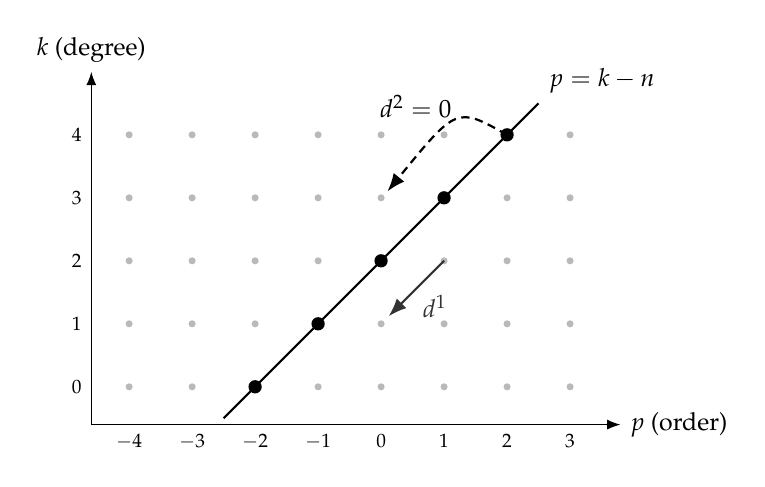
\begin{tikzpicture}[>=Latex,scale=0.8]
  \foreach \p in {-4,...,3}{
    \foreach \k in {0,...,4}{
      \fill[gray!55] (\p,\k) circle (1.6pt);
    }
  }
  \draw[->] (-4.6,-0.6) -- (3.8,-0.6) node[right] {\small \(p\) (order)};
  \draw[->] (-4.6,-0.6) -- (-4.6,5.0) node[above] {\small \(k\) (degree)};
  \foreach \p in {-4,...,3} \node[below] at (\p,-0.6) {\scriptsize \(\p\)};
  \foreach \k in {0,...,4} \node[left] at (-4.6,\k) {\scriptsize \(\k\)};
  \draw[thick] (-2.5,-0.5) -- (2.5,4.5) node[above right] {\small \(p=k-n\)};
  \foreach \k in {0,...,4} \fill (\k-2,\k) circle (3pt);
  \draw[->,thick,gray!40!black] (1,2) -- node[below right=-2pt] {\small \(d^1\)} (0.12,1.12);
  \draw[->,thick,densely dashed] (2,4) .. controls (1.2,4.45) .. (0.1,3.1);
  \node at (0.55,4.45) {\small \(d^2=0\)};
\end{tikzpicture}
\caption[The order spectral sequence]{The spectral sequence of the order
filtration for a symbol algebra, drawn for \(n=2\). Gray dots mark the
positions \((p,k)\) where \(E^1_{p,k}\) (homogeneous \(k\)-forms of degree
\(p\)) can be non-zero. The differential \(d^1\) moves along lines
parallel to \(p=k-n\). After the symplectic star and
Proposition~\ref{prop:homog}, \(E^2\) lives only on the line \(p=k-n\)
(black dots), and the higher differentials leave that line, so they vanish.
Adapted from \cite[Ch.~10]{MelroseMicro}.}
\label{fig:ss}
\end{figure}

\subsection{Morita invariance}\label{subsec:morita}
If \(e\in M_N(\mathfrak A)\) is an idempotent not contained in any proper
two-sided ideal, then \(eM_N(\mathfrak A)e\) is Morita equivalent to
\(\mathfrak A\) and has the same Hochschild homology (B6)
\cite[Prop.~13]{MN}, \cite{Loday}. For matrices and for algebras
\(\mathcal K\widehat\otimes\mathfrak A\) as in Lemma~\ref{lem:Hunital},
with \(\mathfrak A\) unital or only H-unital, the generalized trace
\(\Tr_*\) is a quasi-isomorphism (Lemma~\ref{ha:lem:morita}, adapted from
\cite[Lemma ``Morita invariance for smoothing kernels'']{HHb}). Full
corners are Proposition~\ref{ha:prop:corner}, and the application to
bundles is Remark~\ref{ha:rem:bundles}. We use the smoothing-kernel case with \(\mathcal K=\Psi^{-\infty}(
\partial X)\) to remove the boundary smoothing operators in
Section~\ref{sec:indicial}.

\section{Functions and weighted de Rham cohomology (MN \S1)}
\label{sec:functions}

\begin{question}
Why do MN allow arbitrary negative powers of \(x\), that is, Laurent
coefficients, instead of working with \(\Psic^{\Z}(X)\) itself?
\end{question}
\begin{answer}
For the same reason that one allows operators of all integral orders. The
order filtration and the \(x\)-filtration are treated symmetrically: in
\(x^{-\Z}\Psic^{\Z}\) both \(Q\) and \(x\) are invertible modulo the
residual ideals. The homology is then finite dimensional, and each
filtration contributes a circle, \(\Ssig\) for the order and \(\Sd\) for
the powers of \(x\), with classes \(d\log r\) and \(d\log x\). Without
negative powers, closed forms such as \(\beta\wedge dx/x^2\) would no longer
be exact (Correction~\ref{corr:cdR}), and the homology would acquire
infinite-dimensional pieces, as it does for order zero
(Section~\ref{subsec:other}). On the analytic side, \(x^{-p}A\) has the
same index as \(A\) when both are fully elliptic \cite[p.~31]{MN}, so
nothing is lost.
\end{answer}

Throughout this section \(M\) is a compact manifold with boundary, and
\(x\) is a boundary defining function with a fixed collar
\([0,\epsilon)_x\times\partial M\). We consider the three algebras of the
Taylor sequence \cite[(25)]{MN},
\begin{equation}\label{eq:taylorfun}
 0\to\dCI(M)\to x^{-\Z}\CI(M)\to\CI(\partial M)\Lser{x}\to0,
\end{equation}
where the last map takes the Taylor series at \(\partial M\) in the collar
and \(\CI(\partial M)\Lser{x}\) is the algebra of formal Laurent series
\(\sum_{k\ge-p}f_kx^k\).

\subsection{H-unitality of the flat functions}

\begin{lemma}[MN Lemma 1]\label{lem:flatHunital}
\(\dCI(M)\) is topologically H-unital.
\end{lemma}

\begin{proof}
The \(k\)-chains are \(\dCI(M^{k+1})\). Choose
\(\phi\in\CI_c((-1,1))\) with \(\phi(0)=1\), and for
\(f\in\dCI(M^{k+1})\) define
\begin{equation}\label{eq:E}
 (Ef)(z^{(0)},z^{(1)},\dots,z^{(k+1)})=
 \phi\Bigl(\frac{x^{(0)}-x^{(1)}}{x^{(0)}+x^{(1)}}\Bigr)
 f(z^{(1)},\dots,z^{(k+1)}) ,
\end{equation}
where \(x^{(j)}\) is \(x\) on the \(j\)-th factor \cite[(26)]{MN}.

\emph{\(Ef\) is flat.} Put \(w=(x^{(0)}-x^{(1)})/(x^{(0)}+x^{(1)})\in[-1,1]\).
On the support of \(\phi(w)\) we have \(|w|\le1-\delta\) for some
\(\delta>0\). Hence \(x^{(0)}\) and \(x^{(1)}\) are comparable there:
\(c\,x^{(1)}\le x^{(0)}\le C\,x^{(1)}\). The function \(\phi(w)\) is smooth
away from \(x^{(0)}=x^{(1)}=0\). Each derivative of \(\phi(w)\) is
bounded by a power of \((x^{(0)}+x^{(1)})^{-1}\), which is bounded by a
power of \(1/x^{(1)}\) on the support. Since \(f\) vanishes to infinite
order as \(x^{(1)}\to0\), every derivative of \(Ef\) is
\(O((x^{(1)})^\infty)=O((x^{(0)})^\infty)\) there. At the faces
\(x^{(j)}=0\), \(j\ge1\), flatness is inherited from \(f\). So
\(E:\dCI(M^{k+1})\to\dCI(M^{k+2})\) continuously.

\emph{\(E\) is a contraction.} The face \(d_0\) restricts to
\(z^{(0)}=z^{(1)}\), where \(w=0\), so \(d_0Ef=f\). For \(i\ge1\), the
face \(d_i\) identifies \(z^{(i)}\) and \(z^{(i+1)}\), and does not touch
the factor \(\phi(w)\) unless \(i=1\). When \(i=1\) it replaces \(z^{(1)}\)
by itself, so in all cases \(d_iE=Ed_{i-1}\). Therefore
\[
 b'Ef=d_0Ef+\sum_{i\ge1}(-1)^id_iEf=f-E\Bigl(\sum_{i\ge0}(-1)^id_if\Bigr)
 =f-Eb'f. \qedhere
\]
\end{proof}

\begin{remark}[The support of \(\phi\)]\label{rem:phi}
MN only ask that \(\phi\in\CI_c(\R)\) with \(\phi(0)=1\). This is not
enough. If \(\phi(-1)\ne0\), then at a point with \(x^{(0)}=0<x^{(1)}\)
we have \(w=-1\), and \(Ef=\phi(-1)f(z^{(1)},\dots)\) need not vanish, so
\(Ef\notin\dCI(M^{k+2})\). The support condition \(\supp\phi\subset(-1,1)\)
is what makes \(x^{(0)}\) and \(x^{(1)}\) comparable.
\end{remark}

The algebra \(x^{-\Z}\CI(M)\) is unital, and so is
\(\CI(\partial M)\Lser{x}\). By excision (B4, Theorem~\ref{ha:thm:excision}),
\eqref{eq:taylorfun} gives a long exact sequence in Hochschild homology.

\subsection{Hochschild homology of the three function algebras}
The HKR map \(\chi\) is defined on the chains of all three algebras
\cite[(27)]{MN}:
\begin{align*}
 \chi&:\dCI(M^{k+1})\to\dCI(M;\Lambda^k),\\
 \chi&:x_0^{-\Z}\cdots x_k^{-\Z}\CI(M^{k+1})\to x^{-\Z}\CI(M;\Lambda^k),\\
 \chi&:\CI((\partial M)^{k+1})\Lser{x_0,\dots,x_k}\to
 \CI(\partial M;\Lambda^k)\Lser{x}\oplus\CI(\partial M;\Lambda^{k-1})\Lser{x}
 \,\frac{dx}{x^2} .
\end{align*}
(MN print \(M\) for \(\partial M\) in the last target.) In the last line a
\(k\)-form on the formal neighbourhood of \(\partial M\) is split into its
tangential part and its \(dx\)-part. Any of \(dx\), \(dx/x\), \(dx/x^2\)
may be used as the normal basis element, since the coefficients are Laurent
series. MN use \(dx/x^2\) to match the cusp geometry. We use \(dx/x\) when
computing cohomology.

\begin{lemma}[MN Lemma 2]\label{lem:fun}
The three HKR maps are isomorphisms on Hochschild homology. The long exact
sequence of \eqref{eq:taylorfun} splits into the short exact sequences
\cite[(28)]{MN}
\[
 0\to\dCI(M;\Lambda^k)\to x^{-\Z}\CI(M;\Lambda^k)\to
 \CI(\partial M;\Lambda^k)\Lser{x}\oplus\CI(\partial M;\Lambda^{k-1})\Lser{x}\,
 \frac{dx}{x}\to0 .
\]
\end{lemma}

\begin{proof}
The HKR maps for the three algebras are isomorphisms by
Theorem~\ref{ha:thm:variants} (the flat, Laurent and formal Laurent cases
of (B5)); for \(\C\Lser{x}\) this is the Koszul computation \(\HH_0=
\C\Lser{x}\), \(\HH_1=\C\Lser{x}\,dx\), \(\HH_k=0\) for \(k\ge2\). No
K\"unneth formula for formal Laurent series is needed. The HKR maps
commute with the maps of \eqref{eq:taylorfun}, since restriction to Taylor
series commutes with \(d\) (Theorem~\ref{ha:thm:variants}). Finally, the
right-hand map at the level of forms is surjective by Borel's lemma (every
formal Laurent form is the Taylor series of a Laurent form). So the
connecting maps vanish, and the long exact sequence breaks into the
displayed short exact sequences.
\end{proof}

\subsection{Weighted de Rham cohomology}
The de Rham differential acts on all three spaces of forms in
Lemma~\ref{lem:fun}.

\begin{lemma}[Formal Laurent forms]\label{lem:formaldR}
The cohomology of the de Rham complex of formal Laurent forms
\(\sum_{j\ge-p}x^j(\alpha_j+\beta_j\wedge dx/x)\), with
\(\alpha_j,\beta_j\) forms on \(\partial M\), is
\(H^k(\partial M)\oplus H^{k-1}(\partial M)\,dx/x\). It is spanned by the
classes with \(j=0\).
\end{lemma}

\begin{proof}
For a \(k\)-form \(\alpha\) on \(\partial M\),
\(d(x^j\alpha)=x^j\bigl(d\alpha+(-1)^kj\,\alpha\wedge dx/x\bigr)\), and
\(d(x^j\beta\wedge dx/x)=x^j\,d\beta\wedge dx/x\). So the complex splits
into the subcomplexes of fixed \(x\)-degree \(j\). On degree \(j\) the
differential is
\((\alpha,\beta)\mapsto(d\alpha,\,d\beta+(-1)^kj\alpha)\). This is the
mapping cone of multiplication by \(j\) on the de Rham complex of
\(\partial M\). For \(j\ne0\) that multiplication is invertible, so the
cone is acyclic; explicitly
\(h(\alpha,\beta)=((-1)^{k-1}j^{-1}\beta,0)\) is a contracting homotopy.
For \(j=0\) the complex is the direct sum of the de Rham complex of
\(\partial M\) and its shift.
\end{proof}

\begin{proposition}[MN Proposition 1]\label{prop:dR}
The de Rham cohomology of the three complexes in Lemma~\ref{lem:fun} is
\[
 \Hrel^k(M),\qquad H^k(M)\oplus H^{k-1}(\partial M),\qquad
 H^k(\partial M)\oplus H^{k-1}(\partial M),
\]
and the long exact sequence is \cite[(29)]{MN}
\[
 \cdots\to\Hrel^k(M)\to H^k(M)\oplus H^{k-1}(\partial M)
 \xrightarrow{\ \iota^*\oplus\mathrm{Id}\ }H^k(\partial M)\oplus
 H^{k-1}(\partial M)\to\Hrel^{k+1}(M)\to\cdots ,
\]
the direct sum of the long exact sequence of the pair \((M,\partial M)\)
and the identity on \(H^{k-1}(\partial M)\).
\end{proposition}

\begin{proof}
\emph{Flat forms.} The complex \(\dCI(M;\Lambda^\bullet)\) contains the
compactly supported forms on the interior, and the inclusion is a
quasi-isomorphism \cite[p.~9]{MN}. In the collar a flat form is
\(\alpha+\beta\wedge dx\) with \(\alpha,\beta\) flat at \(x=0\). The
homotopy \(h(\alpha+\beta\wedge dx)=\pm\int_0^x\beta\), integrated from
the boundary and cut off away from the collar, preserves flatness. It
shows that a closed flat form is cohomologous to one that vanishes near
\(\partial M\). The cohomology is therefore \(H_c^k(M^\circ)=\Hrel^k(M)\).

\emph{Formal Laurent forms.} This is Lemma~\ref{lem:formaldR}.

\emph{Laurent forms.} Let \(\chi_0\in\CI(M)\) be a cut-off equal to \(1\)
near \(\partial M\) and supported in the collar. Consider
\[
 \Psi:\CI(M;\Lambda^k)\oplus\CI(\partial M;\Lambda^{k-1})\to
 x^{-\Z}\CI(M;\Lambda^k),\qquad
 (\gamma,\beta)\mapsto\gamma+\chi_0\,\beta\wedge\frac{dx}{x}.
\]
It is a chain map for the differential \((\gamma,\beta)\mapsto(d\gamma,
d\beta)\), because \(d\chi_0\wedge\beta\wedge dx=0\) (\(d\chi_0\) is a
multiple of \(dx\) in the collar). It fits into a map of short exact
sequences: from \cite[(30)]{MN},
\[
 0\to\dCI(M;\Lambda^\bullet)\to\CI(M;\Lambda^\bullet)\oplus
 \CI(\partial M;\Lambda^{\bullet-1})\to\CI(\partial M;\Lambda^\bullet\oplus
 \Lambda^{\bullet-1})\to0,
\]
where the second map is restriction to \(\partial M\) plus the identity, to
the sequence of Lemma~\ref{lem:fun}. On the outer terms the induced maps in
cohomology are the identity and the inclusion of the \(j=0\) part of
Lemma~\ref{lem:formaldR}. Both are isomorphisms, so \(\Psi\) is a
quasi-isomorphism by the five lemma. The cohomology of the source is
\(H^k(M)\oplus H^{k-1}(\partial M)\), by the de Rham theorem for manifolds
with boundary. The long exact sequence of the source sequence is the
sequence of the pair together with the identity on \(H^{k-1}(\partial
M)\).
\end{proof}

\begin{example}\label{ex:interval}
For \(M=[0,1)\) (non-compact, but the computation is local), the Laurent
de Rham cohomology is \(H^0=\C\) and \(H^1=\C\,dx/x\). For the compact
interval \(M=[0,1]\) with \(x=s(1-s)\), it is \(H^0=\C\) and
\(H^1=\C^2\), spanned by \(dx/x\) localized near either end. The relative
cohomology is \(\Hrel^1([0,1])=\C\), and the map
\(\Hrel^1\to H^1\oplus H^0(\partial M)\) is zero, as it must be.
\end{example}

\subsection{b- and cusp de Rham complexes}
The Laurent forms \(x^{-\Z}\CI(M;\Lambda^k)\) coincide with the Laurent
b-forms and the Laurent cusp forms. The smooth b-forms \(\CI(M;{}^b\Lambda^k)\),
locally generated by \(dx/x\) and \(dy\), and the smooth cusp forms
\(\CI(M;{}^c\Lambda^k)\), generated by \(dx/x^2\) and \(dy\), are
subcomplexes \cite[(32)--(33)]{MN}. By the proof of
Proposition~\ref{prop:dR} the b-complex has the cohomology of the Laurent
complex,
\[
 {}^bH^k(M)\cong H^k(M)\oplus H^{k-1}(\partial M)
\]
(Nest--Tsygan \cite{NestTsyganBoundary}, quoted in \cite{MN}).

\begin{correction}[The cusp de Rham complex]\label{corr:cdR}
After \cite[(33)]{MN} it is stated that the cusp de Rham complex also has
cohomology \({}^bH^k(M)\). This is not so: its cohomology is
\[
 {}^cH^k(M)\cong H^k(M)\oplus H^{k-1}(\partial M)\oplus H^{k-1}(\partial M).
\]
The extra classes are \(\beta\wedge dx/x^2\), with \(\beta\) closed on
\(\partial M\). They are exact in the Laurent complex
(\(\beta\wedge dx/x^2=\pm d(\beta/x)\)) but not in the smooth cusp
complex.
\end{correction}

\begin{proof}
Expand a smooth cusp form near \(\partial M\) as
\(\sum_{j\ge0}x^j(\alpha_j+\beta_j\wedge dx/x^2)\). From
\(d(x^j\alpha)=x^j\,d\alpha+(-1)^kj\,x^{j+1}\alpha\wedge dx/x^2\) we see that
the differential pairs \(\alpha_j\) with \(\beta_{j+1}\), with coefficient
\(j\). For \(j\ge1\) this pairing is invertible, and those pairs cancel as
in Lemma~\ref{lem:formaldR}. What survives is \(\alpha_0\), \(\beta_0\)
and \(\beta_1\). Since \(\alpha_{-1}\) is not available, \(\beta_0\) is
not hit. This gives \(H^k(\partial M)\oplus H^{k-1}(\partial M)\oplus
H^{k-1}(\partial M)\) for the formal boundary complex. A form
\(\chi_0\beta\wedge dx/x^2\) with \(d\beta=0\) is closed on \(M\), so the
connecting map vanishes on the new classes, and the five-lemma argument of
Proposition~\ref{prop:dR} gives the result. On \([0,1)\): \(dx/x^2\) and
\(dx/x\) are closed smooth cusp \(1\)-forms, and neither is \(df\) for a
smooth \(f\).
\end{proof}

This plays no role in \cite{MN}, which only uses the Laurent complex.

\subsection{Homogeneous Laurent forms}
Let \(V\to M\) be a real vector bundle and \(r\) a positive function on
\(V\setminus0\), homogeneous of degree one. Combining
Proposition~\ref{prop:homog} with Proposition~\ref{prop:dR} gives
\cite[(35)]{MN}: the de Rham cohomology of formal sums of homogeneous
Laurent forms on \(V\setminus0\), with degrees bounded above, is
\begin{equation}\label{eq:bH}
 {}^bH^k(SV\times\Ssig)={}^bH^k(SV)\oplus{}^bH^{k-1}(SV)\,\frac{dr}r
 \cong H^k(SV\times\Ssig)\oplus H^{k-1}(\partial SV\times\Ssig)\,\frac{dx}x .
\end{equation}
The same holds with flat forms (relative cohomology) and with formal Laurent
forms at the boundary (cohomology of \(\partial SV\times\Ssig\times\Sd\)).

\section{The symbol algebras \texorpdfstring{\(\As\)}{As} and \texorpdfstring{\(\Is\)}{Is} (MN \S2)}\label{sec:symbols}

\begin{proposition}[MN Proposition 2]\label{prop:As}
\(\HH_k(\As)\cong{}^bH^{2n-k}(Y\times\Ssig)\), that is,
\[
 \HH_k(\As)\cong H^{2n-k}(Y)\oplus H^{2n-k-1}(Y)\,d\theta_\sigma\oplus
 H^{2n-k-1}(Z)\,\frac{dx}x\oplus H^{2n-k-2}(Z)\,d\theta_\sigma\wedge
 \frac{dx}x .
\]
Equivalently, \(\HH_k(\As)\cong H^{2n-k}(Y\times\Ssig)\oplus
H^{2n-k-1}(Z\times\Ssig)\), and by duality
\(\HH^k(\As)\cong\Hrel^k(Y\times\Ssig)\oplus H^k(Z\times\Ssig)\).
\end{proposition}

\begin{proof}
\emph{Chains and filtration.} By the quantization (B1,
Proposition~\ref{cc:prop:quant}), as vector spaces,
\[
 \As\cong\varinjlim_{m,N}x^{-N}\prod_{j\le m}\mathcal G^j(\cT),
\]
with the star product \cite[(37)]{MN}. Completing tensor products gives the
chains \cite[(38)]{MN}: formal sums
\(\sum_{p\le P}c_p\), where \(c_p\) is a function on \((\cT\setminus0)^{k+1}\)
with Laurent singularities in each \(x_j\), homogeneous in each factor,
of total homogeneity \(p\). The order filtration is independent of the
quantization, and the Hochschild differential decomposes as
\(b=\sum_lb_l\) with \(b_l\) coming from \(P_l\). So we are in the setting
of Section~\ref{subsec:convergence}.

\emph{\(E^1\).} The differential \(b_0\) is the Hochschild differential of
the commutative algebra \(x^{-\Z}\mathcal G(\cT)\). By
Corollary~\ref{ha:cor:homog} (Connes' theorem (B5) for Laurent functions on
the sphere bundle, with a radial variable), \(E^1_{p,k}\cong
x^{-\Z}\mathcal G^p(\cT;\Lambda^k)\), the homogeneous Laurent \(k\)-forms of
degree \(p\); in the mixed complexes of Remark~\ref{rem:poles} this is
Lemma~\ref{ha:lem:stageE1}.

\emph{\(d^1\).} By Proposition~\ref{prop:d1}, \(d^1=-i\delta\), where
\(\delta\) is the Koszul--Brylinski differential of the cusp Poisson
structure \eqref{eq:poisson}. This is the extension by continuity of the
Poisson differential of the interior \cite[p.~12]{MN}.

\emph{\(E^2\).} The cusp symplectic form is
\(\omega=d\tau\wedge dx/x^2+d\eta\wedge dy\), homogeneous of degree one,
with only a finite order singularity at \(x=0\). The symplectic star
operator therefore maps \(x^{-\Z}\mathcal G^p(\cT;\Lambda^k)\) isomorphically
onto \(x^{-\Z}\mathcal G^{p+n-k}(\cT;\Lambda^{2n-k})\) and intertwines
\(\delta\) with \(\pm d\) (Proposition~\ref{prop:star}). In local
coordinates, \(*(f\,dx^I\,d\zeta^J)=\pm x^{\pm2}f\,dx^{J^\complement}
d\zeta^{I^\complement}\), which explains the factor \(x^2\) in
\cite[p.~12]{MN}. Hence
\[
 E^2_{p,k}\cong H^{2n-k}\bigl(x^{-\Z}\mathcal G^{p+n-k}(\cT;\Lambda^\bullet),
 d\bigr),
\]
which vanishes for \(p\ne k-n\) by Proposition~\ref{prop:homog}. For
\(p=k-n\) it equals \({}^bH^{2n-k}(Y\times\Ssig)\) by \eqref{eq:bH}.

\emph{Degeneration and convergence.} \(E^2\) is concentrated on the line
\(p=k-n\). Proposition~\ref{ha:prop:laurent} then shows that every class
has a representative on that line and that the leading-symbol map
\(\Theta\) is well defined. For \(n=1\), \(\Theta\) is an isomorphism by
Corollary~\ref{ha:cor:n1}. For \(n\ge2\) this is the quoted step (B10)
(Remark~\ref{rem:poles}, Remark~\ref{ha:rem:quoted}).

\emph{Duality.} \(Y\times\Ssig\) is a compact oriented
\(2n\)-manifold with boundary \(Z\times\Ssig\). It is oriented by the
symplectic structure and the orientation of the circle. Lefschetz duality
gives \(H^{2n-k}(Y\times\Ssig)^*\cong\Hrel^k(Y\times\Ssig)\), and
Poincar\'e duality on the closed \((2n-1)\)-manifold \(Z\times\Ssig\) gives
\(H^{2n-k-1}(Z\times\Ssig)^*\cong H^k(Z\times\Ssig)\).
\end{proof}

\begin{discussion}
\textbf{The singular symplectic form.} Over the interior, \(\cT=T^*X\)
and \(\omega\) is the usual symplectic form. At the boundary,
\(\omega=d\tau\wedge dx/x^2+\cdots\) blows up to second order. Its inverse,
the Poisson bivector \(x^2\partial_\tau\wedge\partial_x+\cdots\),
\emph{vanishes} to second order. This is why \(\delta\) extends smoothly
to the boundary and why the commutator of two cusp operators is again a
cusp operator. On Laurent forms the factor \(x^{\pm2}\) is invisible, and
the computation is word for word the closed one. What changes is the
de Rham cohomology of the Laurent forms, which picks up the boundary term
\(H^{*-1}(Z)\,dx/x\) (Proposition~\ref{prop:dR}).
\end{discussion}

\begin{proposition}[MN Proposition 3]\label{prop:Is}
\(\Is\) is H-unital, \(\HH_k(\Is)\cong\Hrel^{2n-k}(Y\times\Ssig)\), and
\(\HH^k(\Is)\cong H^k(Y\times\Ssig)\).
\end{proposition}

\begin{proof}
The computation is that of Proposition~\ref{prop:As} with flat forms in
place of Laurent forms. By Proposition~\ref{prop:dR} these give relative
cohomology. Here no pole orders occur, and convergence is proved in
Theorem~\ref{ha:thm:conv}, using the mixed complexes of
Lemma~\ref{ha:lem:mixed}. For H-unitality, one can filter the bar complex
by order. Its \(E^1\) term is the bar homology of the commutative algebra
\(\dCI\)-valued in homogeneous functions. This vanishes by
Lemma~\ref{lem:flatHunital}, whose contraction \eqref{eq:E} only involves
the base variables and preserves homogeneity. Concluding that the bar
complex of \(\Is\) is acyclic needs completeness, which the chain model
lacks (Remark~\ref{rem:poles}), so we prefer the direct argument: use the
contraction
\eqref{eq:E} directly with a quantization in which \(\mathrm{Id}\) has
full symbol \(1\) and which is a left quantization in the collar. Then
the cut-off factor in \eqref{eq:E} is independent of the fibre variable
in slot \(0\), and \(P_j(\phi(w),\cdot)=0\) for \(j\ge1\)
\cite[p.~13]{MN}.
\end{proof}

\begin{remark}
One can also obtain Proposition~\ref{prop:Is} from the closed case: the
operators with kernels supported in the interior are dense in \(\Is\),
and \(\Is\) is an ideal in \(\Psi^{\Z}(2X)/\Psi^{-\infty}(2X)\) for the
double \(2X\) \cite[(47)]{MN}. In Section~\ref{sec:residues} this
identification shows that \(\Trs\) is Wodzicki's residue.
\end{remark}

\section{The boundary symbol algebra and the boundary sequence (MN \S3)}
\label{sec:boundarysym}

\begin{proposition}[MN Proposition 4]\label{prop:Ads}
\(\HH_k(\Ads)\cong H^{2n-k}(Z\times\Ssig\times\Sd)\) and
\(\HH^k(\Ads)\cong H^k(Z\times\Ssig\times\Sd)\).
\end{proposition}

\begin{proof}
\(\Ads\cong\CI(Z)\Lser{x,q^{-1}}\) (as vector spaces, with the transported
star product) consists of formal Laurent series in \(x\)
of complete symbols over \(\partial X\). The proof of
Proposition~\ref{prop:As} applies with formal Laurent forms on the formal
neighbourhood of \({}^cT^*_{\partial X}X\setminus0\), including its
reliance on (B10) for convergence when \(n\ge2\); for \(n=1\) convergence
is Proposition~\ref{ha:prop:xadic}. The homogeneous
de Rham cohomology is generated over \(H^*(Z)\) by \(1\), \(d\log r\),
\(d\log x\) and \(d\log x\wedge d\log r\) \cite[p.~13]{MN}
(Lemma~\ref{lem:formaldR} and Proposition~\ref{prop:homog}). The total
dimension of \(Z\times\Ssig\times\Sd\) is \(2n\). Since \(Z\times\Ssig
\times\Sd\) is closed, Poincar\'e duality gives the cohomology statement.
\end{proof}

\begin{proposition}[MN Proposition 5]\label{prop:boundaryLES}
The ideal \(\Is\) is H-unital. Under the isomorphisms of
Propositions~\ref{prop:As}, \ref{prop:Is} and \ref{prop:Ads}, the long
exact sequence of \(0\to\Is\to\As\to\Ads\to0\) is the direct sum of the
long exact sequence of the pair \((Y\times\Ssig,Z\times\Ssig)\) (in degrees
\(2n-k\)) and the identity on \(H^{2n-k-1}(Z\times\Ssig)\,dx/x\):
\begin{enumerate}
\item \(\HH_k(\Is)\to\HH_k(\As)\) is \(\iota^*\oplus0\), relative to
absolute cohomology;
\item \(\HH_k(\As)\to\HH_k(\Ads)\) is restriction to \(Z\times\Ssig\) on
the first summand and the identity on the summand with \(dx/x\);
\item the connecting map \(\partial:\HH_k(\Ads)\to\HH_{k-1}(\Is)\) is a
non-zero universal multiple of the de Rham connecting map
\(H^{2n-k}(Z\times\Ssig)\to\Hrel^{2n-k+1}(Y\times\Ssig)\) on the summand
without \(d\theta_\partial\), and vanishes on the summand
\(H^{2n-k-1}(Z\times\Ssig)\,d\theta_\partial\). The multiple is
\((-1)^ki\).
\end{enumerate}
For the leading-symbol maps \(\Theta\) these three statements hold
without any convergence hypothesis. They are statements about the
isomorphisms of Propositions~\ref{prop:As} and~\ref{prop:Ads} for \(n=1\),
and for \(n\ge2\) given (B10).
\end{proposition}

\begin{proof}
Excision applies because \(\Is\) is H-unital (Proposition~\ref{prop:Is}).
The maps in (1) and (2) come from algebra morphisms that preserve the
order filtration. They therefore induce maps of spectral sequences, and on
\(E^2\) they are the maps induced on homogeneous forms by inclusion and
restriction. This gives (1) and (2) \cite[p.~14]{MN}.

For (3), Theorem~\ref{ha:thm:bdry} proves
\(\Theta_{\Is}\circ\partial=(-1)^ki\,(\delta_{\mathrm{dR}}\oplus0)\circ
\Theta_{\partial,\sigma}\), where \(\Theta_{\Is}\) is the isomorphism of
Theorem~\ref{ha:thm:conv} and \(\Theta_{\partial,\sigma}\) the leading-symbol
map of \(\Ads\). In outline: compute \(\partial\) in the mixed complexes,
where \(\Is\) is represented by the kernel \(D\) of the Taylor map. Write a
class of \(\HH_k(\Ads)\) as a cycle \(c\) with leading term \(c_{k-n}\)
on the critical line. Lift \(c\) linearly to a chain \(\tilde c\) of
\(\As\) whose leading term is a \(b_0\)-cycle: Borel's lemma lifts the
formal Laurent form \(\chi(c_{k-n})\) to a Laurent form \(\lambda\), and
HKR turns \(\lambda\) into a cycle. Then \(b\tilde c\in D\) represents
\(\partial[c]\), and its leading term has HKR form
\(\chi(b_1\tilde c_{k-n})=-i\delta\lambda\), a flat form
(Lemma~\ref{ha:lem:connlead}). Through the symplectic star,
\([\delta\lambda]\) is the de Rham connecting map of
\(0\to\text{flat}\to\text{Laurent}\to\text{formal}\to0\) applied to
\(*\chi(c_{k-n})\), up to the sign \((-1)^{k-1}\). On a class
\(\beta\wedge dx/x\) it vanishes, because \(\chi_0\beta\wedge dx/x\) is a
closed lift. If \(\Theta_{\partial,\sigma}\) is an isomorphism, this is
(3); this holds for \(n=1\) (Proposition~\ref{ha:prop:xadic}) and, for
\(n\ge2\), it is (B10).
\end{proof}

\begin{remark}[On the splitting \(s_0\)]\label{rem:s0}
MN prove (3) differently \cite[pp.~14--15]{MN}. They first treat a
product \(X=H\times[0,1]\), with cusp structure given by \(x(1-x)\), and
use the subalgebra of operators commuting with \(x^2(1-x)^2\partial_x\)
to construct a splitting \(s_0:\Ads^{(0)}\to\As\) that is an algebra
morphism. With a cut-off \(\varphi(x)\) the chain map
\(s(f_0\otimes\dots\otimes f_k)=s_0(f_0)\varphi\otimes s_0(f_1)\otimes
\dots\otimes s_0(f_k)\) then satisfies \([b,s]=\sigma\) with
\(\sigma(f_0\otimes\dots)=s_0(f_0)[\varphi,s_0(f_1)]\otimes\cdots\), a
chain supported in the interior, whose leading symbol is
\(-i\iota_{H_\varphi}\) of the leading symbol of the cycle; the general
case follows by naturality. We could not reconstruct \(s_0\) for formal
Laurent series in \(x\): an element of \(\As\) has only finitely many
poles and cannot carry an infinite formal series. No multiplicative
splitting is needed. The proof above (Theorem~\ref{ha:thm:bdry}) uses a
linear lift whose top component is a \(b_0\)-cycle; the failure of the
lift to be multiplicative only affects components two orders down, which
do not enter the leading symbol. The two computations agree: for
\(\eta\) closed, \(d(\varphi\eta)=d\varphi\wedge\eta\) is MN's
\(\pm*(\iota_{H_\varphi}*\eta)\) (Proposition~\ref{prop:star}). MN's
constant \(\imath\) is our \((-1)^ki\) up to the sign conventions for
\(*\). Everything that follows uses only kernels and images, so the
constant plays no further role.
\end{remark}

\section{The indicial algebra \texorpdfstring{\(\Id\)}{Id} (MN \S4)}
\label{sec:indicial}

\subsection{The model: a boundary point}\label{subsec:Idpoint}
Let \(\partial X\) be a point; for instance \(X=[0,1)\). Then
\(\Psis^{-\infty}(\mathrm{pt})\) is the convolution algebra \(\cS(\R_t)\).
By \eqref{eq:Inkernel} it is isomorphic to \(\cS(\R_\tau)\) with
pointwise multiplication, and
\[
 \Id\cong\cS(\R_\tau)\Lser{x},\qquad A\sim\sum_{j\ge-p}x^ja_j(\tau),
\]
with the product determined by the twist (Lemma~\ref{lem:twist}). Let us
make the product explicit to second order. For \(a,b\in\cS(\R_\tau)\)
(elements of \(x\)-degree zero),
\[
 x^ka=ax^k+ik\,x^{k+1}a'+O(x^{k+2}),
\]
since \([x^k,a]=\sum_jx^j[x,a]x^{k-1-j}\) and \([x,a]=ix^2a'+O(x^3)\).

\begin{lemma}[Commutators in \(\Id\)]\label{lem:commutators}
For \(f,g\in\cS(\R_\tau)\) and \(k\in\Z\):
\begin{enumerate}
\item \([f,g]=0\) when both have \(x\)-degree zero;
\item \([x^kf,\,g]=ik\,x^{k+1}g'f+O(x^{k+2})\);
\item \([x^kf,\,x^{-k}g]=ik\,x\,(fg)'+O(x^2)\).
\end{enumerate}
\end{lemma}

\begin{proof}
(1) Translation invariant operators commute. (2)
\([x^kf,g]=x^k[f,g]+[x^k,g]f=ikx^{k+1}g'f+O(x^{k+2})\). (3) Write
\(x^kfx^{-k}=f+ik\,xf'+O(x^2)\) and \(x^{-k}gx^k=g-ik\,xg'+O(x^2)\). Then
\(x^kfx^{-k}g-x^{-k}gx^kf=fg+ikxf'g-gf+ikxg'f+O(x^2)\).
\end{proof}

\begin{proposition}[\(\Id\) for a boundary point]\label{prop:Idpoint}
\(\HH_0(\Id)\cong\C\), detected by
\[
 \Trd(A)=\bTr(a_1)=\frac1{2\pi}\int_{\R}a_1(\tau)\,d\tau ,
\]
where \(a_1\) is the coefficient of \(x^1\). \(\HH_1(\Id)\cong\C\), generated by the cycle
\(a\otimes b\) with \(a,b\) of \(x\)-degree zero and \(\int ab'\,d\tau
\ne0\), and detected by the cocycle
\[
 (i_{\lx}\Trd)(A,B)=\Trd(A[\lx,B]),\qquad
 (i_{\lx}\Trd)(a,b)=\frac i{2\pi}\int_{\R}a(\tau)b'(\tau)\,d\tau .
\]
\(\HH_k(\Id)=0\) for \(k\ge2\), and \(\Id\) is H-unital.
\end{proposition}

\begin{proof}
\emph{Spectral sequence.} Filter by \(x\)-degree. The chains are formal
sums in increasing powers of \(x\), complete in that direction, and \(b\)
raises \(x\)-degree. The associated graded algebra is the commutative
algebra \(\cS(\R_\tau)[x,x^{-1}]\) (a graded piece for each power of
\(x\)). By HKR (B5) for Schwartz and formal Laurent coefficients
(Theorem~\ref{ha:thm:variants}) and Lemma~\ref{lem:fun},
\[
 E^1\cong\bigl\{\text{forms on }\R_\tau\times(\text{punctured formal disc})
 \text{, Schwartz in }\tau\text{, Laurent in }x\bigr\}
 \qquad\text{\cite[(42)]{MN}}.
\]
By Lemma~\ref{lem:twist}, the first differential is \(-i\delta\) for the
Poisson structure \(\{x,\tau\}=-x^2\), whose symplectic form is
\(\omega=d\tau\wedge dx/x^2\) \cite[p.~16]{MN}. The symplectic star
operator in two dimensions is \(*1=\omega\), \(*\omega=1\) and, on
\(1\)-forms, \(*\,d\tau=d\tau\), \(*\,dx=dx\). Indeed
\(dx\wedge*d\tau=\{x,\tau\}\omega=-x^2\,d\tau\wedge dx/x^2=dx\wedge d\tau\).
So
\[
 E^2_k\cong H^{2-k}_{\mathrm{dR}}\bigl(\text{Schwartz-in-}\tau,\
 \text{Laurent-in-}x\text{ forms}\bigr)
 \cong H^{2-k}_c(\R_\tau\times\Sd)\cong H^{1-k}(\Sd),
\]
where the Laurent de Rham cohomology in \(x\) is spanned by \(1\) and
\(dx/x\) (Lemma~\ref{lem:formaldR}) and the Schwartz de Rham cohomology
in \(\tau\) is \(H^1_c(\R)=\C\), detected by \(\int d\tau\). Concretely:
\begin{itemize}
\item in degree \(k=0\), a function \(\sum x^jf_j\) goes to
\(\sum x^jf_j\,d\tau\wedge dx/x^2\), whose class is \(\int f_1\,d\tau\)
times \([d\tau\wedge dx/x]\);
\item in degree \(k=1\), a form \(\sum x^j(g_j\,d\tau+h_j\,dx)\) goes to a
class determined by \(\int g_0\,d\tau\).
\end{itemize}
The \(E^2\) term sits in \(x\)-degree \(1\) for \(k=0\) and in \(x\)-degree
\(0\) for \(k=1\). Higher differentials raise \(x\)-degree by \(r\ge2\)
and lower \(k\) by one, so they vanish. Convergence, i.e.\ that the
component of power \(1-k\) of a suitable representative gives an
isomorphism \(\HH_k(\Id)\to E^2\), is Proposition~\ref{ha:prop:Idconv}.
The point is that the corrections move to higher powers of \(x\). The
proof uses a complete model: the kernel of the full-symbol map between
the mixed complexes of the unital algebras \(\Ad\) and \(\Ads\) of a
boundary point. A cycle in a stage with poles \(\le L\) is treated in the
stage with poles \(\le L+2\). Every primitive then has poles \(\le L+1\),
so all corrections lie in that stage and their sum converges there.
(The obstruction of Example~\ref{ha:ex:obstruction} concerns terms at
the lowest power of a stage, and these never occur.)

\emph{The generators.} Lemma~\ref{lem:commutators}(3) shows directly that
the \(x^1\)-coefficient of a commutator is a derivative, so its integral
vanishes. Hence \(\Trd\) is a trace. Lemma~\ref{lem:commutators}(2) shows
that \(x^{k+1}h\) is a commutator modulo higher order for \(k\ne0\) and
\(h\) a sum of products \(g'f\). Such sums exhaust \(\cS(\R)\). Indeed, if
\(\int h=0\) then \(h=G'\) with \(G\in\cS\); writing \(G=uv\) with
\(u,v\in\cS\) (every Schwartz function is such a product) gives
\(h=u'v+uv'\). And \(\psi'\psi'\) has positive integral for any non-zero
\(\psi\in\cS\). For degree one: \(a\otimes b\)
is a cycle by Lemma~\ref{lem:commutators}(1). By Lemma~\ref{lem:twist}(3),
\([\lx,b]=-x[t,b]+O(x^2)\) and \(\In([t,b])=-ib'\). Hence
\[
 \Trd(a[\lx,b])=\bTr\bigl(-a[t,b]\bigr)=-\frac1{2\pi}\int a(-ib')\,d\tau
 =\frac i{2\pi}\int ab'\,d\tau .
\]
This is non-zero for suitable \(a,b\), so \(i_{\lx}\Trd\) is a non-zero
class (it is a cocycle by Lemma~\ref{lem:iD}).

\emph{H-unitality.} The same filtration applied to the bar complex has
\(E^1\) equal to the bar homology of the commutative graded algebra. That
algebra is H-unital: it is \(\cS(\R)\otimes\C[x,x^{-1}]\), and
\(\cS(\R)=\cS(\R)\cdot\cS(\R)\) has the contraction
\((Ef)(\tau',\tau_0,\dots)=\phi(\tau'-\tau_0)f(\tau_0,\dots)\) with
\(\phi\in\cS(\R)\) equal to \(1\) near \(0\). Hence \(E^1=0\), and the bar
complex of \(\Id\) is acyclic by completeness. With \(\phi\equiv1\) near
\(0\), the same \(E\) is in fact a contraction for the twisted product:
all derivatives of \(\phi(\tau'-\tau_0)\) vanish on the diagonal, so the
twist corrections of Lemma~\ref{lem:twist} do not contribute to
\(d_0E\).
\end{proof}

\begin{figure}[htbp]
\centering
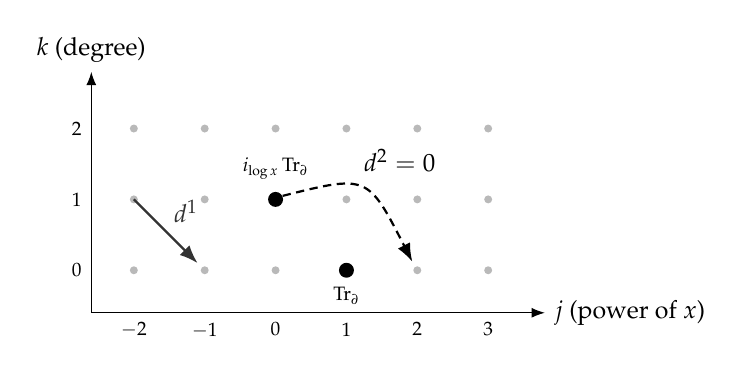
\begin{tikzpicture}[>=Latex,scale=0.9]
  \foreach \j in {-2,...,3}{
    \foreach \k in {0,1,2}{
      \fill[gray!55] (\j,\k) circle (1.6pt);
    }
  }
  \draw[->] (-2.6,-0.6) -- (3.8,-0.6) node[right] {\small \(j\) (power of \(x\))};
  \draw[->] (-2.6,-0.6) -- (-2.6,2.8) node[above] {\small \(k\) (degree)};
  \foreach \j in {-2,...,3} \node[below] at (\j,-0.6) {\scriptsize \(\j\)};
  \foreach \k in {0,1,2} \node[left] at (-2.6,\k) {\scriptsize \(\k\)};
  \fill (1,0) circle (3pt); \fill (0,1) circle (3pt);
  \node[font=\scriptsize,anchor=north] at (1,-0.1) {\(\Trd\)};
  \node[font=\scriptsize,anchor=south] at (0,1.15) {\(i_{\lx}\Trd\)};
  \draw[->,thick,gray!40!black] (-2,1) -- node[above right=-1pt] {\small \(d^1\)} (-1.1,0.1);
  \draw[->,thick,densely dashed] (0.1,1.05) .. controls (1.3,1.35) .. (1.93,0.12);
  \node at (1.75,1.55) {\small \(d^2=0\)};
\end{tikzpicture}
\caption[The \(x\)-adic spectral sequence for \(\Id\)]{The \(x\)-adic
spectral sequence of Proposition~\ref{prop:Idpoint} (one boundary point).
Gray dots: \(E^1\), forms on \(\R_\tau\times\Sd\) of fixed \(x\)-degree
\(j\). The first differential \(d^1=-i\delta\) raises \(j\) by one and
lowers \(k\) by one. \(E^2\) survives only at \((j,k)=(1,0)\), dual to
\(\Trd\), and at \((0,1)\), dual to \(i_{\lx}\Trd\). A differential
\(d^r\) goes from \((j,k)\) to \((j+r,k-1)\), so for \(r\ge2\) it misses
both positions.}
\label{fig:ssId}
\end{figure}

\subsection{General boundary}\label{subsec:Idgeneral}
In a product collar, the variable \(x=1/t\) commutes with operators acting
only in \(y\). Hence, componentwise,
\[
 \Id\cong\bigoplus_{j=1}^N\Psi^{-\infty}(H_j)\widehat\otimes
 \bigl(\cS(\R_\tau)\Lser{x}\bigr)\qquad\text{\cite[p.~16]{MN}}.
\]
Since \(\Psi^{-\infty}(H)=\CI(H)\widehat\otimes\CI(H)\) is of the form
in Lemma~\ref{lem:Hunital}, Morita invariance for smoothing kernels
(Lemma~\ref{ha:lem:morita}) removes it. MN use the Künneth formula
\cite{Karoubi} for the same purpose.

\begin{proposition}[MN Proposition 6, for \(N\) components]\label{prop:Id}
\(\Id\) is H-unital, and
\[
 \HH_k(\Id)\cong\bigoplus_{j=1}^NH^{1-k}(\Sd).
\]
That is, \(\HH_0(\Id)\cong\HH_1(\Id)\cong\C^N\), and
\(\HH_k(\Id)=0\) for \(k\ge2\). The dual bases are
\(\{\Tr_{\partial,j}\}\) and \(\{i_{\lx}\Tr_{\partial,j}\}\), where
\(\Tr_{\partial,j}(A)=\bTr(A_{(1)}|_{H_j})\) \cite[Lemma~10]{MN}.
\end{proposition}

\begin{correction}[Several boundary components]\label{corr:components}
\cite[(16), Prop.~6, Lemma~12]{MN} assert \(\HH^k(\Id)\cong\C\) for
\(k=0,1\). This holds only if \(\partial X\) is connected, which is never
stated, although MN allow disconnected boundary in Appendix~A and use two
boundary components in the proof of their Proposition~5. In general the
answer is \(\C^N\) (Proposition~\ref{prop:Id}). The consequences for
\(\Ad\) and \(\cA\) are worked out in Section~\ref{sec:AdA}. The algebras
\(\Ad\), \(\Ads\) and \(\Id\) are direct sums over the components, so for
them nothing else changes. For \(\cA\), the boundary map
\(\HH^1(\Id)\to\HH^2(\As)\) has rank \(N-1\), not \(0\)
(Proposition~\ref{prop:HHA}).
\end{correction}

\subsection{The residual ideal and the Laurent smoothing operators}

\begin{proposition}\label{prop:I}
\(\cI\) is H-unital, \(\HH_0(\cI)\cong\C\) via the trace and
\(\HH_k(\cI)=0\) for \(k>0\) \cite[end of \S4]{MN}. Moreover, for
\(x^{-\Z}\Psic^{-\infty}(X)\),
\[
 \HH_0\cong\C^N,\qquad\HH_1\cong\C^{N-1},\qquad\HH_k=0\ (k\ge2),
\]
and the connecting map \(\HH_1(\Id)\to\HH_0(\cI)\) is dual to
\(\Tr\mapsto-\sum_ji_{\lx}\Tr_{\partial,j}\).
\end{proposition}

\begin{proof}
\(\cI=\dCI(X)\widehat\otimes\dCI(X)\), so the first part is
Lemma~\ref{lem:Hunital}. For the second part, apply
Lemma~\ref{lem:conn} to \(0\to\cI\to x^{-\Z}\Psic^{-\infty}\to\Id\to0\).
Extend the trace by the \emph{cusp trace}
\(\Tr_c(A)=\FP_{z=0}\Tr(Ax^z)\), the constant term at \(z=0\). For
\(\operatorname{Re}z\) large,
\[
 \Tr([A,B]x^z)=\Tr(A[B,x^z])=-z\,\Tr\bigl(AL(z)x^z\bigr),\qquad
 L(z)=\frac{x^zBx^{-z}-B}{z},\quad L(0)=[\lx,B].
\]
Since \(\Tr(AL(z)x^z)\) has at most a simple pole at \(z=0\) with residue
\(\Trd(AL(0))\), we get \(\Tr_c([A,B])=-\Trd(A[\lx,B])\). This vanishes if
\(A\) or \(B\) is in \(\cI\). So the image of \([\Tr]\) is
\(-\sum_ji_{\lx}\Tr_{\partial,j}\), which is non-zero on every component
by Proposition~\ref{prop:Idpoint}. The connecting map
\(\HH_1(\Id)=\C^N\to\HH_0(\cI)=\C\) is therefore surjective. The long
exact sequence gives the result.
\end{proof}

This is the cusp counterpart of the b-trace defect formula and of part
(iii) of the main theorem of \cite{HHb}. MN do not state it; we include it
because it is the simplest place where the rank \(N-1\) appears.

\section{The residue functionals (MN \S5)}\label{sec:residues}

Fix \(x\) and a positive, elliptic, invertible \(Q\in\Psic^1(X)\)
(Remark~\ref{rem:cuspmetric}). All the trace functionals of \cite{MN} come
from one meromorphic function of two variables.

\subsection{The double zeta function}

\begin{definition}[MN (43)]
For \(A\in x^p\Psic^m(X)\) put
\[
 Z(A;s,z)=Z_{x,Q}(A;s,z)=\tfrac12\bigl(\Tr(Ax^zQ^{-s})+\Tr(AQ^{-s}x^z)\bigr),
 \qquad Z^L(A;s,z)=\Tr(Ax^zQ^{-s}).
\]
\end{definition}

By (B3) (Theorem~\ref{tr:thm:mero}), \(Z\) is holomorphic for
\(\operatorname{Re}z>-p+1\) and \(\operatorname{Re}s>m+n\). It extends meromorphically, with at most
simple poles on the lines \(z=-p+1-j\) and \(s=m+n-k\), \(j,k\in\N_0\)
\cite[Lemma~4]{MN}. The reason for the shift \(-p+1\) in \(z\) is that the
cusp density is \(x^{-2}dx\,\nu_\partial\): the integral \(\int_0x^{z+p}
x^{-2}dx\) converges for \(\operatorname{Re}z>1-p\). Near the origin
\(sz\,Z(A;s,z)\) is holomorphic, and we write \cite[(44)]{MN}
\begin{equation}\label{eq:44}
 sz\,Z(A;s,z)=\Trds(A)+s\,\hTrd(A)+z\,\hTrs(A)+O\bigl(|s|^2+|z|^2\bigr).
\end{equation}
Thus:
\begin{itemize}
\item \(\Trds(A)\) is the coefficient of \((sz)^{-1}\), the \emph{double
residue};
\item \(\hTrd(A)\) is the residue in \(z\) of the regular part in \(s\);
it regularizes the boundary trace by \(Q\);
\item \(\hTrs(A)\) is the residue in \(s\) of the regular part in \(z\);
it is the Wodzicki residue regularized at the boundary by \(x\).
\end{itemize}
\begin{question}
Why are two complex parameters needed?
\end{question}
\begin{answer}
An operator in \(x^{-\Z}\Psic^{\Z}\) fails to be trace class for two
independent reasons: its order may be too large, which is a divergence
of the kernel at the diagonal, and its kernel may not decay at the
boundary, which is a divergence of the integral over the cusp end
\(\int^\infty dt\). The factor \(Q^{-s}\) cures the first and \(x^z\) the
second. The two filtrations have their own residual ideals \(\Is\) and
\(\Id\), and their own residues \(\Trs\) and \(\Trd\). The double residue
\(\Trds\) is the residue of a residue, and it lives on the doubly
quotient algebra \(\Ads\). It is the trace dual to the top class of
\(Z\times\Ssig\times\Sd\): it picks the coefficient of \(x^1\) (the residue
in \(x\), because \(x\cdot dx/x^2=dx/x\)) and the homogeneity \(-n\) (the
residue in the fibre).
\end{answer}

On the diagonal \(s=z\) we get \(\widetilde Z(A;z)=Z(A;z,z)\), with
\[
 z^2\widetilde Z(A;z)=\Trds(A)+z\bigl(\hTrd+\hTrs\bigr)(A)+O(z^2).
\]
Figure~\ref{fig:poles} shows the picture.

\begin{figure}[htbp]
\centering
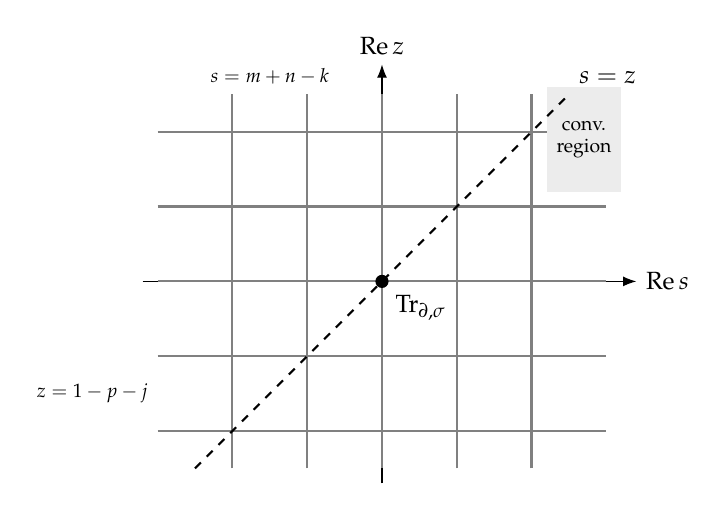
\begin{tikzpicture}[>=Latex,scale=0.95]
 \draw[->] (-3.2,0)--(3.4,0) node[right] {\small \(\operatorname{Re}s\)};
 \draw[->] (0,-2.7)--(0,2.9) node[above] {\small \(\operatorname{Re}z\)};
 \foreach \a in {-2,-1,0,1,2}{
   \draw[thick,gray] (\a,-2.5)--(\a,2.5);
 }
 \foreach \b in {-2,-1,0,1,2}{
   \draw[thick,gray] (-3,\b)--(3,\b);
 }
 \fill[gray!15] (2.2,1.2) rectangle (3.2,2.6);
 \node[font=\scriptsize,align=center] at (2.7,1.9) {conv.\\region};
 \draw[dashed,thick] (-2.5,-2.5)--(2.5,2.5) node[above right] {\small \(s=z\)};
 \fill (0,0) circle (2.5pt);
 \node[font=\small,anchor=north west] at (0.05,-0.05) {\(\Trds\)};
 \node[font=\scriptsize,anchor=south] at (-1.5,2.5) {\(s=m+n-k\)};
 \node[font=\scriptsize,anchor=east] at (-3,-1.5) {\(z=1-p-j\)};
\end{tikzpicture}
\caption[Poles of the double zeta function]{The poles of \(Z(A;s,z)\) lie
on the gray lines (drawn schematically through the origin; after shifting
\(A\) by powers of \(x\) and \(Q\), lines pass through \((0,0)\)). The
crossing at the origin produces the double residue \(\Trds\). The residue
along the line \(z=0\) and the residue along \(s=0\), each regularized in
the other variable, give \(\hTrd\) and \(\hTrs\). Restricting to the
diagonal \(s=z\) gives a double pole with leading coefficient \(\Trds\).}
\label{fig:poles}
\end{figure}

\begin{lemma}[MN Lemma 5]\label{lem:LR}
\(Z^L(A;s,z)-Z(A;s,z)\) is holomorphic near \((0,0)\). Hence the three
functionals in \eqref{eq:44} are the same for \(Z\), \(Z^L\) and
\(Z^R=\Tr(AQ^{-s}x^z)\).
\end{lemma}

\begin{proof}
By the trace property for \(\operatorname{Re}\) large,
\(Z^R-Z^L=\Tr(A[Q^{-s},x^z])\), and
\[
 [Q^{-s},x^z]=\bigl(Q^{-s}x^zQ^sx^{-z}-1\bigr)x^zQ^{-s}.
\]
The family \(Q^{-s}x^zQ^sx^{-z}-1\) is entire of order \(0\) and vanishes
on both axes \(s=0\) and \(z=0\). So it equals \(sz\,M(s,z)\) with \(M\)
entire of order \(0\). Then \(Z^R-Z^L=sz\Tr(AMx^zQ^{-s})\), which has no
pole at the origin, since \(\Tr(AMx^zQ^{-s})\) has at most simple poles in
each variable. Finally \(Z=\frac12(Z^L+Z^R)\).
\end{proof}

\begin{lemma}[MN Lemma 6]\label{lem:Trds}
\(\Trds\) is a trace on \(x^{-\Z}\Psic^{\Z}(X)\). It does not depend on
\(x\) or \(Q\), and it vanishes on \(\Is+\Id\). Hence it defines a trace
on \(\cA\), \(\As\), \(\Ad\) and \(\Ads\).
\end{lemma}

\begin{proof}
\emph{Trace.} By Lemma~\ref{lem:LR} we may use \(Z^L\). For
\(\operatorname{Re}\) large,
\[
 Z^L([A,B])=\Tr(A[B,x^zQ^{-s}])=\Tr\bigl(AK(s,z)x^zQ^{-s}\bigr),\qquad
 K=B-x^zQ^{-s}BQ^sx^{-z}.
\]
The family \(K\) is entire, of fixed order, and vanishes at \((0,0)\).
Hence \(K=sK_1+zK_2\) with \(K_1,K_2\) entire. This is Hadamard's lemma in
two variables, \(K_1=\int_0^1\partial_sK(\theta s,\theta z)\,d\theta\), and
similarly for \(K_2\). Then
\[
 sz\,Z^L([A,B])=s\cdot sz\Tr(AK_1x^zQ^{-s})+z\cdot sz\Tr(AK_2x^zQ^{-s}),
\]
and both brackets are holomorphic near \(0\). So the value at \((0,0)\) is
\(0\).

\emph{Independence.} If \(x'=ax\), then \(x'^z=x^z(1+zB(z))\) with
\(B(z)=(a^z-1)/z\) entire. So \(sz(Z^L_{x'}-Z^L_x)=z\cdot sz\Tr(AB(z)x^z
Q^{-s})\) vanishes at the origin. The case of \(Q\) is the same, with
\(Q'^{-s}=(1+sC(s))Q^{-s}\).

\emph{Vanishing.} If \(A\in x^\infty\Psic^{\Z}\), then \(Ax^z\) is entire
in \(z\) with values in a fixed space of flat operators. So \(Z\) has no
pole in \(z\), and \(\Trds(A)=0\). If \(A\in x^{-\Z}\Psic^{-\infty}\), then
\(Z\) has no pole in \(s\).
\end{proof}

\subsection{The interior residue \texorpdfstring{\(\Trs\)}{Tr-sigma}}
If \(A\in\Is\), then \(Z\) is entire in \(z\). Its residue in \(s\) is
\(\Trs(A)=\Res_{s=0}\Tr(AQ^{-s})\), and \(\hTrs\) restricts to \(\Trs\)
on \(\Is\).

\begin{lemma}[MN Lemma 7 and Proposition 7]\label{lem:Trs}
\(\Trs\) is the extension by continuity of Wodzicki's residue on the
double \(2X\). If \(\sum_ja_j\) is the full symbol of \(A\in\Is\), then
\[
 \Trs(A)=(2\pi)^{-n}\int_{\Y}a_{-n}\,{}^c\nu ,
\]
where \({}^c\nu\) is the contraction of \(\omega^n\) with the radial
vector field. Since \({}^c\nu=x^{-2}\nu'\) with \(\nu'\) smooth, the same
formula defines \(\Trs\) on \(x^p\Psic^{\Z}\) for \(p>1\).
\end{lemma}

\begin{proof}
For \(A\) with kernel supported in \((X^\circ)^2\), choose \(Q'\in
\Psi^1(2X)\) positive and elliptic with \(Q'A-QA\) smoothing. Then
\(\Tr(AQ^{-s})-\Tr(AQ'^{-s})\) is regular at \(0\), so \(\Trs(A)=\TrR(A)\).
Such operators are dense in \(\Is\), and both sides are continuous. The
formula is the local formula (B8) (Theorems~\ref{tr:thm:res}
and~\ref{tr:thm:mero}(1)). The singular density \(x^{-2}\) comes
from \(\omega^n\), which contains \(dx/x^2\).
\end{proof}

\subsection{The double residue}
For general \(A\in x^{-\Z}\Psic^{\Z}(X)\) the function \(\Trs(x^zA)\) is
defined for \(\operatorname{Re}z\) large and is meromorphic in \(z\)
\cite[(52)]{MN}.

\begin{lemma}[MN Lemma 8]\label{lem:Trdsformula}
\(\Trds(A)=\Res_{z=0}\Trs(x^zA)\). Explicitly,
\[
 \Trds(A)=(2\pi)^{-n}\int_{\Zb}a_{-n,(1)}\,{}^c\nu_\partial ,
\]
where \(a_{-n,(1)}\) is the term of homogeneity \(-n\) in the symbol of
the coefficient \(A_{(1)}\) of \(x^1\) in \eqref{eq:taylor}, and
\({}^c\nu_\partial\) is the density on \(\Zb\) obtained by contracting
\(\omega_\partial^{n-1}d\tau\) with the radial field on
\({}^cT^*_{\partial X}X=T^*\partial X\times\R_\tau\).
\end{lemma}

\begin{proof}
By the definitions, \(\Trds(A)\) is the \(z\)-residue of the \(s\)-residue,
which is \(\Res_z\Trs(x^zA)\). Insert the formula of Lemma~\ref{lem:Trs}:
\(\int_0x^{z}\,x^j\,x^{-2}dx\) has a pole at \(z=0\) only for \(j=1\), with
residue \(1\).
\end{proof}

\begin{example}[A boundary point]\label{ex:Trdspoint}
Let \(n=1\) and let \(A=x\,c(D_t)\) near the boundary point, with
\(c\) a classical symbol. The kernel of \(xc(D_t)Q^{-s}\) on the diagonal
is \(x\cdot(2\pi)^{-1}\int c(\tau)\langle\tau\rangle^{-s}d\tau\), and the
cusp density is \(dt=dx/x^2\). So
\[
 \Res_z\int_0^1x^{1+z}\frac{dx}{x^2}=1,\qquad
 \Trds(A)=\frac1{2\pi}\bigl(c_{-1}(1)+c_{-1}(-1)\bigr),
\]
where \(c\sim c_{-1}(\pm1)|\tau|^{-1}\) as \(\tau\to\pm\infty\). The two
points of \(Z=\{\tau=\pm1\}\) contribute separately, \emph{with positive
weights}. The density \({}^c\nu_\partial\) is a density, not a form.
\end{example}

\begin{example}[The four functionals on the half-line]\label{ex:four}
Let \(n=1\), and near the boundary point let \(A=\varphi(x)\,x^k\,c(D_t)\),
where \(\varphi\) is a cut-off equal to \(1\) near \(x=0\), \(c\) is a
classical symbol of order \(m\), and \(Q\) is translation invariant near
the boundary with \(q=\langle\tau\rangle\). The diagonal value of the
kernel of \(x^kc(D_t)Q^{-s}\) is \(x^k(2\pi)^{-1}\int c(\tau)\langle\tau
\rangle^{-s}d\tau\). Integrating against \(x^z\,dx/x^2\) gives
\[
 Z(A;s,z)\approx\Bigl(\int_0^1\varphi\,x^{k+z-2}\,dx\Bigr)\cdot
 \frac1{2\pi}\int_{\R}c(\tau)\langle\tau\rangle^{-s}\,d\tau ,
\]
up to terms that are holomorphic near the origin. The first factor has a
pole at \(z=0\) only if \(k=1\), with residue \(1\). The second factor has
a pole at \(s=0\) with residue \((2\pi)^{-1}(c_{-1}(1)+c_{-1}(-1))\), and
regular value \(\bTr(c)+\gamma'(0)/2\pi\) (Proposition~\ref{prop:Tr8}).
Writing \(c\sim\sum_jc^\pm_j|\tau|^j\) as \(\tau\to\pm\infty\) and
expanding \(\langle\tau\rangle^{-s}=|\tau|^{-s}\sum_l\binom{-s/2}{l}
\tau^{-2l}\), one finds \(\gamma'(0)=\sum_{l\ge1}\frac{(-1)^l}{2l}
(c^+_{2l-1}+c^-_{2l-1})\). So, for \(k=1\),
\begin{gather*}
 \Trds(A)=\frac{c_{-1}(1)+c_{-1}(-1)}{2\pi},\qquad
 \hTrd(A)=\bTr(c)+\frac{\gamma'(0)}{2\pi},\\
 \hTrs(A)=\FP_{z=0}\!\int_0^1\varphi\,x^{z-1}dx\cdot\Trds(A),
\end{gather*}
and for \(k\ne1\), \(\Trds(A)=\hTrd(A)=0\). The correction vanishes if
\(c\) has order \(\le0\); for \(c=\langle\tau\rangle\) it is
\(-1/2\pi\) (Example~\ref{tr:ex:counter}). This illustrates
Lemma~\ref{lem:Trdsformula} and Corollary~\ref{cor:Tr61}. The functional
\(\hTrs\) is a residue in the fibre variable with a Hadamard finite part
in \(x\), and \(\hTrd\) is a regularized trace in the fibre variable with
a residue in \(x\).
\end{example}

\begin{correction}[Dimension one]\label{corr:n1}
For \(n=1\) the set \(Z_j\) consists of two points, \(\tau=\pm1\), over
each boundary point. Then \(\Trds\) splits as \(\Trds^++\Trds^-\), and
each summand is a trace (the proof of Lemma~\ref{lem:Trds} applies with a
cut-off in \(\tau\)). Hence \(\HH^0(\As)\cong\HH^0(\Ads)\cong\C^{2N}\),
and similarly \(\HH^0(\Is)\cong H^0(Y\times\Ssig)\cong\C^2\) for connected
\(X\). The statements ``\(\HH^0\) is one-dimensional'' after
\cite[(16)]{MN} and \cite[Lemma~12]{MN} require \(n\ge2\), exactly as
Wodzicki's uniqueness of the residue does. The cohomological formulas of
Theorem~\ref{thm:main} for \(\Is\), \(\As\), \(\Ads\) remain true for
\(n=1\), with \(Z_j\) disconnected. For \(n=1\) they do not depend on the
quoted step (B10) (Corollary~\ref{ha:cor:n1}).
\end{correction}

\subsection{The regularized interior residue \texorpdfstring{\(\hTrs\)}{}}
By Lemma~\ref{lem:Trdsformula}, \(\hTrs(A)\) is the regular value at
\(z=0\) of \(\Trs(x^zA)\). Equivalently, it is the Hadamard finite part
\cite[(55)]{MN}:
\begin{equation}\label{eq:55}
 \hTrs(A)=\lim_{\epsilon\downarrow0}\Bigl((2\pi)^{-n}\int_{\Y\cap\{x>\epsilon\}}
 a_{-n}\,{}^c\nu+(\log\epsilon)\Trds(A)+\sum_{l>0}\gamma_l\epsilon^{-l}\Bigr).
\end{equation}
The sign of the logarithm is right, since \(\int_\epsilon^1x^{-1}dx=
-\log\epsilon\).

\begin{lemma}[MN Lemma 9]\label{lem:hTrs}
\(\hTrs\) vanishes on \(\Id\), does not depend on \(Q\), and for \(x'=ax\)
\[
 \hTrs(A;x')-\hTrs(A;x)=\Trds\bigl(A\log a\bigr).
\]
\end{lemma}

\begin{proof}
The residue \(\Trs\) vanishes on smoothing operators and does not depend on
\(Q\). For the change of \(x\), \(\Trs((x'^z-x^z)A)=\Trs(zx^zB(z))\) with
\(B(z)=z^{-1}(a^z-1)A\) entire (MN print \(A^z\) for \(a^z\)). Its value
at \(z=0\) is \(\Res_z\Trs(x^zB(z))=\Trds(B(0))=\Trds(A\log a)\).
\end{proof}

\subsection{The boundary trace and the regularized suspended trace}

\begin{lemma}[MN Lemma 10]\label{lem:Trd}
On \(\Id\), \(\Trd(A)=\Res_{z=0}\Tr(Ax^z)=\bTr(A_{(1)})\), where
\(\bTr(B)=(2\pi)^{-1}\int\Tr\In(B,\tau)\,d\tau\) \cite[(57)]{MN}. It is a
trace and does not depend on \(x\) or \(Q\).
\end{lemma}

\begin{proof}
On the diagonal of \(X_c^2\) the kernel of \(A\) is \(B\,\nu\) with
\(\nu=x^{-2}\nu'\), and \(B\in x^{-\Z}\CI(X)\). Write
\(B\sim\sum_kx^kB_{(k)}\). The residue at \(z=0\) of
\(\int x^zB\,x^{-2}dx\,\nu_\partial\) comes from \(k=1\) and equals
\(\int_{\partial X}B_{(1)}\nu_\partial\). This is the kernel of
\(A_{(1)}\) at \(\{0\}\times\Delta_{\partial X}\) integrated over the
boundary, which is \(\bTr(A_{(1)})\) by Fourier inversion
(Theorem~\ref{tr:thm:mero}(2)). The trace property was proved in
Proposition~\ref{prop:Idpoint}. Independence is as in
Lemma~\ref{lem:Trds}.
\end{proof}

Melrose's regularization of \(\bTr\) to all of \(\Psis^{\Z}(H)\)
\cite{MelroseEta}, \cite[(58)--(59)]{MN}, takes \(p\) large, integrates
\(h_p(\tau)=\Tr(\partial_\tau^pB(\tau))\) \(p\) times from \(0\), and takes
\((2\pi)^{-1}\) times the constant term of \(\int_{-T}^T\) as
\(T\to\infty\) (Definition~\ref{tr:def:bTr}). It does not depend on \(p\),
it vanishes on odd families, and it is a trace on \(\Psis^{\Z}(H)\)
(Theorem~\ref{tr:thm:bTr}).

\begin{proposition}[MN Proposition 8, corrected]\label{prop:Tr8}
Let \(Q_0=(D_t^2+\Delta_H+1)^{1/2}\), or more generally let \(Q_0(s)\) be a
holomorphic suspended family of order \(-s\) with \(Q_0(0)=\mathrm{Id}\).
For \(B\in\Psis^m(H)\), the function \(\bTr(BQ_0^{-s})\) (defined by the
integral for \(\operatorname{Re}s\) large) is meromorphic, and
\[
 s\,\bTr(BQ_0^{-s})=\widetilde{\Tr}(B)+s\Bigl(\bTr(B)+\frac{\gamma_B'(0)}
 {2\pi}\Bigr)+O(s^2),
\]
where \(\widetilde\Tr(B)=(2\pi)^{-n}\int b_{-n}\) is the Wodzicki residue of
\(B\) regarded as an operator on \(\R\times H\) (\(n=\dim H+1\)), and
\(\gamma_B(s)\) is the sum over \(\tau\to\pm\infty\) of the coefficients of
\(|\tau|^{-1-s}\) in the fibre integral over \(T^*H\) of the symbol of
\(BQ_0^{-s}\) (before integration the relevant term has homogeneity
\(-n-s\)). The correction \(\gamma_B'(0)\) is local, and it
is not zero in general.
\end{proposition}

\begin{proof}
This is Theorem~\ref{tr:thm:susreg} with \(C(s)=BQ_0^{-s}\). The residue is
\(\gamma_B(0)/2\pi=\widetilde\Tr(B)\). For the regular value one compares
the \(p\)-fold integration by parts in the definition of \(\bTr\) with the
continuation in \(s\); the boundary terms produce \(\gamma_B'(0)\).
\cite[Prop.~8]{MN} omits this term. For \(H\) a point and
\(B=\langle D_t\rangle\), \(\gamma_B(s)=1-s\), so the regular value is
\(\bTr(B)-1/2\pi\) (Example~\ref{tr:ex:counter}).
\end{proof}

\begin{remark}[The functional in MN Proposition 8]\label{rem:Prop8}
MN write the residue as \(\widetilde\Tr(B)=\bTr([t,B])\). This cannot be
right as it stands. Take \(H=\mathrm{pt}\) and \(B=\langle D_t\rangle^{-1}\).
The residue is \((2\pi)^{-1}(1+1)=1/\pi\), whereas \(\In([t,B])=
-i\partial_\tau\langle\tau\rangle^{-1}\) is odd, so \(\bTr([t,B])=0\). (In
general \(\bTr([t,B])\) picks out the difference of the
\(|\tau|^0\)-coefficients at \(\pm\infty\), not the \(|\tau|^{-1}\)
coefficients.) Only the residue description is used later, through
Corollary~\ref{cor:Tr61}, so we take it as the definition. The other claim
of \cite[Prop.~8]{MN}, about the regular value, is corrected in
Proposition~\ref{prop:Tr8} (item~\ref{item:Prop8reg} of
Section~\ref{subsec:errata}).
\end{remark}

\begin{corollary}[MN Corollaries 1 and 2; (2) corrected]\label{cor:Tr61}
For \(A\in x^{-\Z}\Psic^{\Z}(X)\):
\begin{enumerate}
\item \(\Trds(A)=\widetilde\Tr(A_{(1)})\), the residue of
\(\Trd(AQ^{-s})\) at \(s=0\) \cite[(61)]{MN};
\item if \(Q\) is translation invariant to all orders at \(\partial X\),
with Taylor series \(Q_0^{-s}\) at the front face, then
\[
 \hTrd(A)=\bTr(A_{(1)})+\frac{\gamma'_{A_{(1)}}(0)}{2\pi},
\]
with the local correction \(\gamma_{A_{(1)}}\) of
Proposition~\ref{prop:Tr8}, computed from \(A_{(1)}Q_0^{-s}\). \cite{MN}
state this without the correction term.
\end{enumerate}
\end{corollary}

\begin{proof}
If \(Q\) is translation invariant to all orders, then
\((AQ^{-s})_{(1)}=A_{(1)}Q_0^{-s}\), and by Lemma~\ref{lem:LR} and
Theorem~\ref{tr:thm:mero}(2), \(\hTrd(A)\) is the regular value at \(s=0\)
of \(\bTr(A_{(1)}Q_0^{-s})\). Proposition~\ref{prop:Tr8} applies
(Correction~\ref{tr:corr:Prop8}). In general the residue does not depend
on \(Q\).
\end{proof}

\begin{lemma}[MN Lemma 11]\label{lem:hTrdQ}
For two regularizers \(Q\), \(Q'\),
\[
 \hTrd(A;Q')-\hTrd(A;Q)=-\Trds\bigl(A\log(Q'/Q)\bigr),\qquad
 \log(Q'/Q)=\frac{d}{ds}Q'^sQ^{-s}\Big|_{s=0}\in\Psic^0(X).
\]
\end{lemma}

\begin{proof}
Write \(Q'^{-s}=(1+sB(s))Q^{-s}\) with \(B(s)=s^{-1}(Q'^{-s}Q^s-1)\), so
that \(B(0)=-\log(Q'/Q)\). Then
\(\Trd(AQ'^{-s})-\Trd(AQ^{-s})=s\Trd(AB(s)Q^{-s})\). Its value at \(s=0\)
is \(\Res_s\Trd(AB(0)Q^{-s})=\Trds(AB(0))\).
\end{proof}

Thus \(\hTrd\) does not depend on \(x\) but does depend on \(Q\), while
\(\hTrs\) does not depend on \(Q\) but does depend on \(x\).

\section{Exterior derivations and explicit cocycles (MN \S\S6--7)}
\label{sec:derivations}

\subsection{The two derivations}
The derivations are \cite[(63)--(64)]{MN}
\[
 D_{\lQ}A=[\lQ,A]=\frac{d}{ds}Q^sAQ^{-s}\Big|_{s=0},\qquad
 D_{\lx}A=[\lx,A]=\frac{d}{dz}x^zAx^{-z}\Big|_{z=0}.
\]
On symbols, \(\sigma([\lQ,A])=-i\{\log q,a\}\) lowers the order by one.
Similarly \(\sigma([\lx,A])=-i\{\log x,a\}=i\,x\,\partial_\tau a\), which
lowers the order by one and raises the power of \(x\) by one, by
\eqref{eq:poisson}. Both derivations preserve \(\cI\), \(\Is\), \(\Id\).
Changing \(Q\) or \(x\) changes them by inner derivations, so the induced
maps \(i_{\lQ}\), \(i_{\lx}\) are canonical (Lemma~\ref{lem:iD}).

\begin{lemma}\label{lem:TrdsD}
\(\Trds([\lQ,B])=\Trds([\lx,B])=0\) for all \(B\) \cite[(84)]{MN}.
\end{lemma}

\begin{proof}
Put \(Q^uBQ^{-u}=B+uM(u)\), with \(M\) entire and \(M(0)=[\lQ,B]\). By the
trace property, for \(\operatorname{Re}\) large,
\[
 \Tr\bigl(Q^uBQ^{-u}x^zQ^{-s}\bigr)=\Tr\bigl(Bx^z(x^{-z}Q^{-u}x^zQ^u)
 Q^{-s}\bigr).
\]
The family \(x^{-z}Q^{-u}x^zQ^u-1\) vanishes for \(u=0\) and for \(z=0\),
so it equals \(uz\,N(u,z)\) with \(N\) entire. Comparing the two sides,
\(u\,Z^L(M(u);s,z)=uz\Tr(Bx^zNQ^{-s})\), so
\(Z^L(M(0);s,z)=z\Tr(Bx^zN(0,z)Q^{-s})\). Multiplying by \(sz\) and
evaluating at the origin gives \(\Trds([\lQ,B])=0\). For \(\lx\), put
\(x^wBx^{-w}=B+wL(w)\) and use
\(\Tr(x^wBx^{-w}x^zQ^{-s})=\Tr\bigl(Bx^z(x^{-w}Q^{-s}x^wQ^s)Q^{-s}\bigr)\),
where now \(x^{-w}Q^{-s}x^wQ^s-1=ws\,P(w,s)\). The same argument gives
\(\Trds([\lx,B])=0\). This is \cite[(84)]{MN}, where only the combination
\([\lx-\lQ,B]\) is treated.
\end{proof}

\subsection{Traces generate degree zero}

\begin{lemma}[MN Lemma 12, for \(N\) components, \(n\ge2\)]\label{lem:HH0}
\(\HH^0(\Is)=\C\,\Trs\). Moreover \(\HH^0(\As)\) and \(\HH^0(\Ads)\) are
spanned by the double residues \(\Tr_{\partial,\sigma,j}\) of the
components (the restriction of \(\Trds\) to \(Z_j\)), and \(\HH^0(\Id)\)
is spanned by the \(\Tr_{\partial,j}\).
\end{lemma}

\begin{proof}
By Theorem~\ref{thm:main} and Propositions~\ref{prop:As}--\ref{prop:Id},
the dimensions are \(1\), \(N\), \(N\), \(N\). The functionals listed are
traces (Lemmas~\ref{lem:Trds}, \ref{lem:Trs}, \ref{lem:Trd}, applied
componentwise), and they are linearly independent: by
Example~\ref{ex:Trdspoint} and Proposition~\ref{prop:Idpoint} each one is
non-zero on an element supported near a single component.
\end{proof}

\subsection{The isomorphisms \texorpdfstring{\(\Phi_j\)}{Phi} and the action of the derivations}
Using Lefschetz and Poincar\'e duality as in Proposition~\ref{prop:As},
the homology computations give isomorphisms \cite[(65)--(68)]{MN}
\begin{align*}
 \Phi_1&:H^*(Z\times\Ssig)\oplus\Hrel^*(Y\times\Ssig)\to\HH^*(\As),&
 \Phi_2&:H^*(Y\times\Ssig)\to\HH^*(\Is),\\
 \Phi_3&:H^*(Z\times\Ssig\times\Sd)\to\HH^*(\Ads),&
 \Phi_4&:H^*(\Sd)^{\oplus N}\to\HH^*(\Id).
\end{align*}
(MN print \(S^*M\) for \(Y\) in (65).) The class \(\Phi(\eta)\) is
characterized by its values on antisymmetric chains \cite[(69)]{MN}:
\begin{equation}\label{eq:69}
 \Phi([\eta])\bigl(\mathsf A(f_0\otimes\dots\otimes f_p)\bigr)=
 \int*\bigl(\chi_0(f_0\otimes\dots\otimes f_p)\bigr)\wedge\eta ,
\end{equation}
where \(\chi_0\) is the HKR map on principal symbols and \(\mathsf A\) is
antisymmetrization. MN normalize the circle classes as
\(d\theta_\sigma=[i\,dr/r]\) and \(d\theta_\partial=[i\,dx/x]\). The factor
\(i\) absorbs the \(-i\) in \(\sigma([\cdot,\cdot])=-i\{\cdot,\cdot\}\).

\begin{proposition}[MN Proposition 9]\label{prop:Phi}
\(i_{\lQ}\Phi_j(\xi)=\Phi_j(d\theta_\sigma\wedge\xi)\) for \(j=1,2,3\), and
\(i_{\lx}\Phi_j(\xi)=\Phi_j(d\theta_\partial\wedge\xi)\) for \(j=3,4\).
\end{proposition}

\begin{proof}
Choose \(Q\) with principal symbol \(r\). On leading symbols,
\(i_{\lQ}\) replaces \(f_0\otimes f_1\otimes\cdots\) by
\(f_0\sigma([\lQ,f_1])\otimes\cdots=-if_0H_{\log r}f_1\otimes\cdots\). After
antisymmetrization this gives
\[
 \chi_0\circ i_{\lQ}\circ\mathsf A=-i\,\iota_{H_{\log r}}\circ\chi_0
 \circ\mathsf A .
\]
By Proposition~\ref{prop:star}, \(\iota_{H_f}*\eta'=\pm*(df\wedge\eta')\).
Inserting this into \eqref{eq:69} moves \(d\log r\) onto \(\eta\), which
is wedge with \(d\theta_\sigma\) up to MN's normalization. The same
argument with \(\log x\) gives \(d\theta_\partial\) on the boundary
algebras, where \(x\) is a variable of the symplectic space. On \(\As\)
and \(\Is\) the derivation \(i_{\lx}\) is not of this form, because
\(\log x\) is singular at the boundary.
\end{proof}

\subsection{Explicit cocycles}
For \(\Id\) the degree one generator is \(i_{\lx}\Trd\). Its value on
translation invariant elements was computed in
Proposition~\ref{prop:Idpoint}. In general, by Lemma~\ref{lem:twist}(3),
\[
 (i_{\lx}\Trd)(B,C)=-\sum_{k\ge1}\frac1k\,\Trd\bigl(B\,x^k\,
 \mathrm{ad}_t^k(C)\bigr),
\]
and only finitely many terms contribute to the coefficient of \(x^1\).
\cite[(70)]{MN} gives a kernel formula for this cocycle. We were not able
to match its index conventions with \cite[Lemma~10]{MN}: with
\(A\sim\sum x^{-j}A_j\) the products \(B_{-j}C_{j-k}\) in (70) have total
power \(x^k\), not \(x^1\). We therefore use the formula above.

For the symbol algebras, MN describe cocycles
\(\tau_b(g_0,\dots,g_p)=\Trs(f_0g_0[f_1,g_1]\cdots[f_p,g_p])\) built from
chains \(b=f_0\otimes\dots\otimes f_p\). When \(\chi_0(b)\) represents
\(\eta\), the class of \(\tau_b\) is \(\Phi_2([\eta])\). Composing with
\(i_{\lQ}\) and \(i_{\lx}\) gives the classes with \(d\theta_\sigma\) and
\(d\theta_\partial\) \cite[p.~24]{MN}. We do not need these beyond degree
two.

\section{The homology of \texorpdfstring{\(\Ad\)}{Ad} and \texorpdfstring{\(\cA\)}{A} (MN \S8)}
\label{sec:AdA}

\subsection{The boundary maps of the traces: MN (17)}

\begin{lemma}[MN Lemma 13]\label{lem:17}
For \(A,B\in x^{-\Z}\Psic^{\Z}(X)\),
\begin{align*}
 \hTrd([A,B])&=\Trds(A[\lQ,B])=(i_{\lQ}\Trds)(A,B),\\
 \hTrs([A,B])&=-\Trds(A[\lx,B])=-(i_{\lx}\Trds)(A,B).
\end{align*}
(MN print \(i_{\log r}\) in the second line.)
\end{lemma}

\begin{proof}
\emph{First line.} \(\hTrd(C)\) is the regular value at \(s=0\) of
\(\Trd(CQ^{-s})\), by Lemma~\ref{lem:LR}. For \(C=[A,B]\),
\[
 \Trd([A,B]Q^{-s})=\Trd(A[B,Q^{-s}])=s\,\Trd\bigl(AM(s)Q^{-s}\bigr),
 \qquad M(s)=\frac{B-Q^{-s}BQ^s}s ,
\]
using that \(\Trd=\Res_z\Tr(\cdot\,x^z)\) is a trace on operators of order
below \(-n\). Since \(M(0)=[\lQ,B]\), the regular value at \(s=0\) is
\(\Res_s\Trd(A[\lQ,B]Q^{-s})=\Trds(A[\lQ,B])\) by
Corollary~\ref{cor:Tr61}.

\emph{Second line.} \(\hTrs(C)\) is the regular value at \(z=0\) of
\(\Trs(Cx^z)\). Since \(\Trs\) is a trace,
\[
 \Trs([A,B]x^z)=\Trs(A[B,x^z])=-z\,\Trs\bigl(AL(z)x^z\bigr),\qquad
 L(z)=\frac{x^zBx^{-z}-B}z ,
\]
with \(L(0)=[\lx,B]\). The regular value is
\(-\Res_z\Trs(A[\lx,B]x^z)=-\Trds(A[\lx,B])\) by
Lemma~\ref{lem:Trdsformula}.
\end{proof}

Both right-hand sides vanish if \(A\) or \(B\) lies in \(\Is+\Id\). By
Lemma~\ref{lem:conn}, Lemma~\ref{lem:17} computes the connecting maps of
\(0\to\Id\to\Ad\to\Ads\to0\) and \(0\to\Is\to\As\to\Ads\to0\) on the
traces \cite[(17)--(19)]{MN}. The corresponding statements hold for each
boundary component separately. Figure~\ref{fig:traces} puts
Lemma~\ref{lem:17} next to the other trace defects of these notes.

\begin{figure}[htbp]
\centering
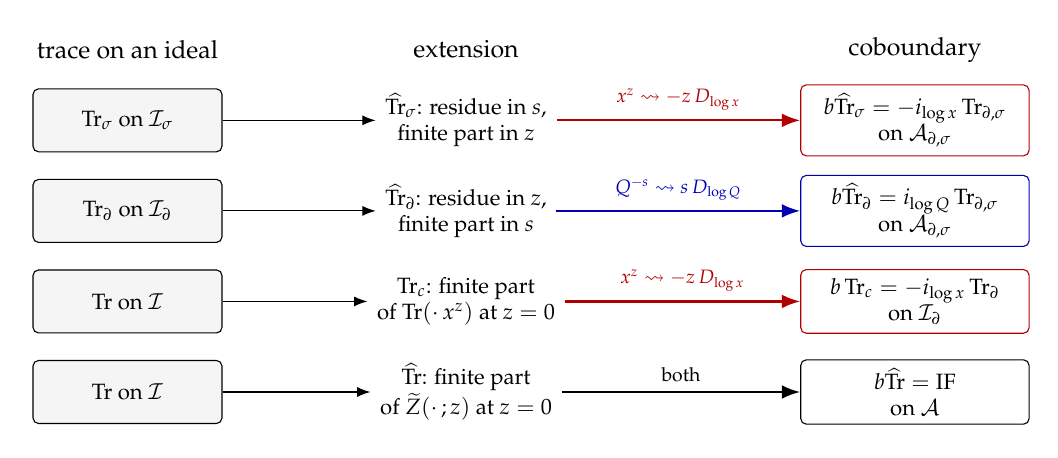
\begin{tikzpicture}[>=Latex,font=\footnotesize,
  tr/.style={draw,rounded corners=2pt,fill=gray!8,align=center,inner sep=3pt,
    minimum height=8mm,minimum width=2.4cm},
  ex/.style={align=center},
  co/.style={draw,rounded corners=2pt,align=center,inner sep=3pt,
    minimum height=8mm,minimum width=2.9cm}]
 \node[font=\small] at (0,0.9) {trace on an ideal};
 \node[font=\small] at (4.3,0.9) {extension};
 \node[font=\small] at (10.0,0.9) {coboundary};
 \foreach \r/\a/\b/\c/\d/\col in {
   0/{\(\Trs\) on \(\Is\)}/{\(\hTrs\): residue in \(s\),\\ finite part in \(z\)}/{\(b\hTrs=-i_{\lx}\Trds\)\\ on \(\Ads\)}/{\(x^z\leadsto-z\,D_{\lx}\)}/red,
   1/{\(\Trd\) on \(\Id\)}/{\(\hTrd\): residue in \(z\),\\ finite part in \(s\)}/{\(b\hTrd=i_{\lQ}\Trds\)\\ on \(\Ads\)}/{\(Q^{-s}\leadsto s\,D_{\lQ}\)}/blue,
   2/{\(\Tr\) on \(\cI\)}/{\(\Tr_c\): finite part\\ of \(\Tr(\cdot\,x^z)\) at \(z=0\)}/{\(b\Tr_c=-i_{\lx}\Trd\)\\ on \(\Id\)}/{\(x^z\leadsto-z\,D_{\lx}\)}/red,
   3/{\(\Tr\) on \(\cI\)}/{\(\widehat\Tr\): finite part\\ of \(\widetilde Z(\cdot\,;z)\) at \(z=0\)}/{\(b\widehat\Tr=\IF\)\\ on \(\cA\)}/{both}/black}{
   \node[tr] (a\r) at (0,-1.15*\r) {\a};
   \node[ex] (b\r) at (4.3,-1.15*\r) {\b};
   \node[co,draw=\col!70!black] (c\r) at (10.0,-1.15*\r) {\c};
   \draw[->] (a\r)--(b\r);
   \draw[->,thick,\col!70!black] (b\r)--node[above,font=\scriptsize]{\d}(c\r);
 }
\end{tikzpicture}
\caption[Extensions of traces and their coboundaries]{Every boundary map
in \cite{MN} is computed by Lemma~\ref{lem:conn}: extend a trace from an
ideal by analytic continuation, then take the Hochschild coboundary
\((b\varphi)(A,B)=\varphi([A,B])\). Commuting past the regularizer produces a
derivation: \([B,Q^{-s}]=s\,M(s)Q^{-s}\) with \(M(0)=[\lQ,B]\), and
\([B,x^z]=-z\,L(z)x^z\) with \(L(0)=[\lx,B]\). The factor \(s\) or \(z\)
cancels the pole, leaving a residue of \(A\,D(B)\). Rows 1--2:
Lemma~\ref{lem:17} \cite[(17)]{MN}; their sum is
\(\Bf=(i_{\lQ}-i_{\lx})\Trds\) (Proposition~\ref{prop:Bf}). Row~3:
Proposition~\ref{prop:I}. Row~4: Lemma~\ref{lem:fedosov} and
Proposition~\ref{prop:IF}, where both derivations occur through
\(\widetilde D=[\lx-\lQ,\cdot\,]\).}
\label{fig:traces}
\end{figure}

\subsection{The algebra \texorpdfstring{\(\Ad\)}{Ad}}
Since \(\Id\) is H-unital, \(0\to\Id\to\Ad\to\Ads\to0\) gives a long
exact sequence. By Proposition~\ref{prop:Id} it reduces in cohomology to
\cite[(71)--(72)]{MN}
\begin{gather*}
 0\to\HH^0(\Ads)\to\HH^0(\Ad)\to\HH^0(\Id)\xrightarrow{\partial}
 \HH^1(\Ads)\to\HH^1(\Ad)\to\cdots\\
 \cdots\to\HH^1(\Id)\xrightarrow{\partial}\HH^2(\Ads)\to\HH^2(\Ad)\to0,
\end{gather*}
together with \(\HH^k(\Ad)\cong\HH^k(\Ads)\) for \(k\ge3\).

\begin{proposition}[MN Proposition 10]\label{prop:10}
For each component \(H_j\),
\[
 \partial[\Tr_{\partial,j}]=[i_{\lQ}\Tr_{\partial,\sigma,j}],\qquad
 \partial[i_{\lx}\Tr_{\partial,j}]=-[i_{\lx}i_{\lQ}\Tr_{\partial,\sigma,j}],
\]
and both maps \(\partial\) are injective.
\end{proposition}

\begin{proof}
The first formula is Lemma~\ref{lem:17} with Lemma~\ref{lem:conn},
applied to the extension \(\hTrd\) of \(\Trd\). For the second, the
cochain \(i_{\lx}\hTrd\) extends \(i_{\lx}\Trd\), and by
Lemma~\ref{lem:iD}
\[
 b(i_{\lx}\hTrd)=-i_{\lx}(b\hTrd)=-i_{\lx}i_{\lQ}\Trds .
\]
This vanishes when one argument is in \(\Id\), because \(\Trds\)
vanishes on \(\Id\) and \(\Id\) is an ideal preserved by both
derivations. By Proposition~\ref{prop:Phi}, under \(\Phi_3\) the two
images are \(d\theta_\sigma\cdot1_{Z_j}\) and \(-d\theta_\partial\wedge
d\theta_\sigma\cdot1_{Z_j}\). These are linearly independent over \(j\),
and non-zero because each \(Z_j\) is non-empty.
\end{proof}

\begin{proposition}[MN Proposition 11]\label{prop:Ad}
\(\HH^k(\Ad)\cong\HH^k(\Ads)/\C^N\) for \(k=1,2\), and
\(\HH^k(\Ad)\cong\HH^k(\Ads)\) otherwise. Dually, \(\HH_k(\Ad)\) is the
kernel of \(\partial:\HH_k(\Ads)\to\HH_{k-1}(\Id)\) for \(k=1,2\)
\cite[(75)]{MN}.
\end{proposition}

\begin{proof}
Insert the injectivity of Proposition~\ref{prop:10} into the exact
sequence.
\end{proof}

\subsection{The algebra \texorpdfstring{\(\cA\)}{A}}
Now consider \(0\to\Id\to\cA\to\As\to0\) \cite[(77)]{MN}. The quotient
maps give a morphism of extensions to \(0\to\Id\to\Ad\to\Ads\to0\). By
naturality of the connecting maps,
\begin{equation}\label{eq:natural}
 \partial_{\cA}=p^*\circ\partial_{\Ad}:\HH^i(\Id)\to\HH^{i+1}(\As),
 \qquad p:\As\to\Ads .
\end{equation}

\begin{lemma}[The map \(p^*\)]\label{lem:pstar}
Write \(\HH^k(\Ads)\cong H^k(Z\times\Ssig)\oplus H^{k-1}(Z\times\Ssig)\,
d\theta_\partial\) and \(\HH^k(\As)\cong\Hrel^k(Y\times\Ssig)\oplus
H^k(Z\times\Ssig)\). Then \(p^*\) is the identity from the first summand
to the second, and \(\pm\delta\) from the \(d\theta_\partial\)-summand to
\(\Hrel^k\). Here \(\delta:H^{k-1}(Z\times\Ssig)\to\Hrel^k(Y\times\Ssig)\)
is the de Rham connecting map.
\end{lemma}

\begin{proof}
\(p^*\) is dual to \(p_*:\HH_k(\As)\to\HH_k(\Ads)\), which is restriction
plus the identity on the \(d\theta_\partial\)-part
(Proposition~\ref{prop:boundaryLES}). Under Poincar\'e duality on
\(Z\times\Ssig\times\Sd\) the summand without \(d\theta_\partial\) in
homology pairs with the summand with \(d\theta_\partial\) in cohomology, and
conversely. The dual of restriction \(H^{2n-k}(Y\times\Ssig)\to
H^{2n-k}(Z\times\Ssig)\) under Lefschetz and Poincar\'e duality is
\(\pm\delta\), by Stokes' theorem:
\(\int_{Z}a|_Z\wedge b=\pm\int_Y a\wedge d(\chi_0\tilde b)\) for closed
\(a\) and \(b\). This is the content of the computation in the proof of
\cite[Prop.~12]{MN}, where it is written \(i\oplus(-1)^q\partial\).
\end{proof}

\begin{proposition}[MN Proposition 12, corrected]\label{prop:HHA}
Let \(X\) be connected and \(n\ge2\). Then:
\begin{enumerate}
\item \(\partial_{\cA}[\Tr_{\partial,j}]=[i_{\lQ}\Tr_{\partial,\sigma,j}]
\leftrightarrow d\theta_\sigma\cdot1_{Z_j}\in H^1(Z\times\Ssig)\), and
\(\partial_{\cA}\) is injective on \(\HH^0(\Id)\);
\item \(\partial_{\cA}[i_{\lx}\Tr_{\partial,j}]=\pm\Phi_1\bigl(\delta
(d\theta_\sigma\cdot1_{Z_j})\bigr)\), and \(\partial_{\cA}\) has rank
\(N-1\) on \(\HH^1(\Id)\), with kernel spanned by
\(\sum_ji_{\lx}\Tr_{\partial,j}=i_{\lx}\Trd\).
\end{enumerate}
Consequently \(\HH^k(\cA)\) is as stated in Theorem~\ref{thm:main}.
\end{proposition}

\begin{proof}
(1) By \eqref{eq:natural}, Proposition~\ref{prop:10} and
Lemma~\ref{lem:pstar}, the image is the class \(d\theta_\sigma\cdot
1_{Z_j}\) in the summand \(H^1(Z\times\Ssig)\) of \(\HH^1(\As)\). These are
independent.

(2) Similarly the image is \(\pm\delta(d\theta_\sigma\cdot1_{Z_j})\). By
exactness of \(H^1(Y\times\Ssig)\to H^1(Z\times\Ssig)\xrightarrow{\delta}
\Hrel^2(Y\times\Ssig)\), a combination \(\sum_jc_jd\theta_\sigma1_{Z_j}\)
lies in \(\ker\delta\) if and only if it is the restriction of a class on
\(Y\times\Ssig\). By the Künneth decomposition \(H^1(Y\times\Ssig)=
H^1(Y)\oplus H^0(Y)\,d\theta_\sigma\), and restriction preserves it.
Since \(Y\) is connected (\(n\ge2\)), \(H^0(Y)=\C\), and the restriction of
\(d\theta_\sigma\) is \(\sum_jd\theta_\sigma1_{Z_j}\). So
\(\ker\delta\cap\operatorname{span}\{d\theta_\sigma1_{Z_j}\}\) is the line
\(c_1=\dots=c_N\), and the rank is \(N-1\).

For the groups, insert (1) and (2) into the exact sequence of
\(0\to\Id\to\cA\to\As\to0\):
\begin{align*}
 \HH^0(\cA)&\cong\HH^0(\As)\cong\C^N,\\
 \HH^1(\cA)&\cong\HH^1(\As)/\C^N\oplus\ker\bigl(\partial_{\cA}|_{\HH^1(\Id)}\bigr)
 \cong\Hrel^1(Y\times\Ssig)\oplus H^1(Z\times\Ssig)/\C^N\oplus\C,\\
 \HH^2(\cA)&\cong\HH^2(\As)/\C^{N-1},\qquad
 \HH^k(\cA)\cong\HH^k(\As),\ k\ge3 .
\end{align*}
The splitting in degree one depends on a choice of extension of
\(i_{\lx}\Trd\) to \(\cA\). One choice is \(-\IF\)
(Section~\ref{sec:index}).
\end{proof}

\begin{correction}[MN Proposition 12]\label{corr:Prop12}
MN find \(\partial[i_{\lx}\Trd]=0\), because ``the form
\(d\theta_\sigma\) has an extension to the whole manifold''
\cite[p.~27]{MN}. That argument is correct for the \emph{sum}
\(\sum_jd\theta_\sigma1_{Z_j}\), which is all there is when \(N=1\). For
\(N\ge2\) the individual classes \(d\theta_\sigma1_{Z_j}\) do not extend,
and \(\HH^2(\cA)\) is smaller than \cite[(16)]{MN} claims by
\(N-1\) dimensions. The same rank appears in the b-calculus
\cite[Remark ``Several boundary components'']{HHb}. If \(X\) has \(c\)
components, each with non-empty boundary, the rank is \(N-c\).
Figure~\ref{fig:rank} illustrates the count.
\end{correction}

\begin{figure}[htbp]
\centering
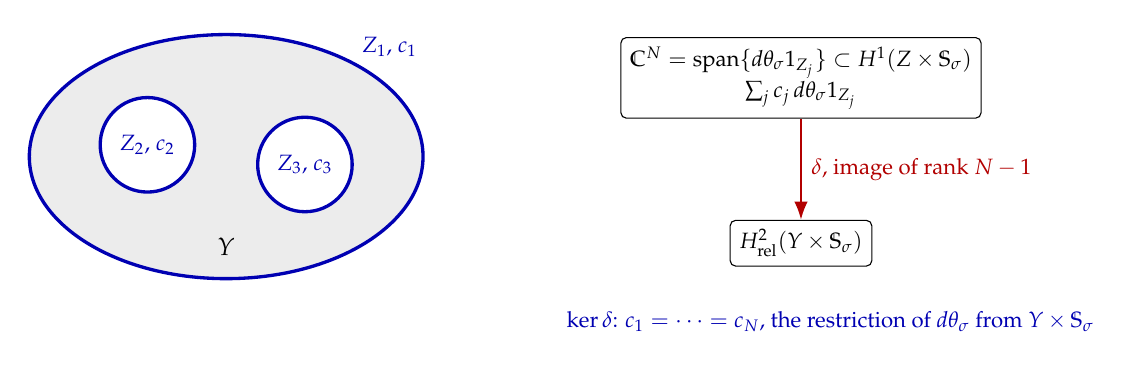
\begin{tikzpicture}[>=Latex,font=\footnotesize]
 \fill[gray!15,even odd rule] (0,0) ellipse (2.5 and 1.55)
   (-1.0,0.15) circle (0.6) (1.0,-0.1) circle (0.6);
 \draw[very thick,blue!70!black] (0,0) ellipse (2.5 and 1.55);
 \draw[very thick,blue!70!black] (-1.0,0.15) circle (0.6);
 \draw[very thick,blue!70!black] (1.0,-0.1) circle (0.6);
 \node at (0,-1.15) {\small \(Y\)};
 \node[blue!70!black,anchor=south west] at (1.6,1.15) {\(Z_1\), \(c_1\)};
 \node[blue!70!black] at (-1.0,0.15) {\(Z_2\), \(c_2\)};
 \node[blue!70!black] at (1.0,-0.1) {\(Z_3\), \(c_3\)};
 \begin{scope}[xshift=7.3cm]
  \node[draw,rounded corners=2pt,align=center] (src) at (0,1.0)
    {\(\C^N=\operatorname{span}\{d\theta_\sigma1_{Z_j}\}\subset H^1(Z\times\Ssig)\)\\
     \(\textstyle\sum_jc_j\,d\theta_\sigma1_{Z_j}\)};
  \node[draw,rounded corners=2pt] (tgt) at (0,-1.1) {\(\Hrel^2(Y\times\Ssig)\)};
  \draw[->,thick,red!70!black] (src)--node[right]{\(\delta\), image of rank \(N-1\)}(tgt);
  \node[align=left,anchor=west,blue!70!black] at (-3.1,-2.1)
    {\(\ker\delta\): \(c_1=\dots=c_N\), the restriction of \(d\theta_\sigma\) from \(Y\times\Ssig\)};
 \end{scope}
\end{tikzpicture}
\caption[The rank \(N-1\) phenomenon]{Why \(\HH^1(\Id)\to\HH^2(\As)\)
has rank \(N-1\) (Proposition~\ref{prop:HHA}, Correction~\ref{corr:Prop12}),
drawn schematically for \(N=3\), with the connected manifold \(Y\) shown as a
planar domain whose boundary \(Z\) has components \(Z_1,Z_2,Z_3\). The class
\(i_{\lx}\Tr_{\partial,j}\) goes to \(\pm\Phi_1(\delta(d\theta_\sigma1_{Z_j}))\),
where \(\delta\) is the de Rham connecting map. A combination
\(\sum_jc_jd\theta_\sigma1_{Z_j}\) lies in \(\ker\delta\) exactly when it
is the restriction of a class on \(Y\times\Ssig\); since \(Y\) is connected
(\(n\ge2\)) this means \(c_1=\dots=c_N\). Dually, by Stokes' theorem,
\(\sum_j\int_{Z_j}\beta=0\) for every closed \(\beta\) on \(Y\). The
kernel is spanned by \(i_{\lx}\Trd=\sum_ji_{\lx}\Tr_{\partial,j}\); MN's
argument sees only this sum.}
\label{fig:rank}
\end{figure}

\begin{discussion}
\textbf{How the index formula comes out of the boundary maps.} The index
functional is a class in \(\HH^1(\cA)\) whose restrictions to the two
ideals are known: \(i_{\lQ}\Trs\) on \(\Is\) (Atiyah--Singer) and
\(-i_{\lx}\Trd\) on \(\Id\) (Toeplitz). A pair of cocycles on the two
ideals extends to \(\cA\) only if their images in \(\HH^2(\Ads)\) agree.
By Lemma~\ref{lem:17} and Proposition~\ref{prop:10}, both images equal
\([i_{\lx}i_{\lQ}\Trds]\). The extension is unique up to the image of
\(\HH^1(\As)\) and \(\HH^1(\Ad)\), and analytic continuation picks one:
the regularized value of \(\widetilde Z([A,B];z)\). Evaluating it on
\([A]\otimes[A^{-1}]\) splits the index into an interior symbolic term
and a boundary indicial term (Section~\ref{sec:index}).
\end{discussion}

\subsection{The full operator algebra}
The ideal \(\cI\) is H-unital with \(\HH_*(\cI)=\C\) in degree \(0\)
(Proposition~\ref{prop:I}). The connecting map
\(\HH_1(\cA)\to\HH_0(\cI)=\C\) is the index functional, which is non-zero:
there are fully elliptic operators of non-zero index
(Example~\ref{ex:interval-index}). Hence
\(\HH_k(x^{-\Z}\Psic^{\Z}(X))\cong\HH_k(\cA)\) for \(k\ne1\), and
\(\HH_1(x^{-\Z}\Psic^{\Z}(X))=\ker\IF\subset\HH_1(\cA)\). This completes
the proof of Theorem~\ref{thm:main}.

\subsection{Examples}\label{subsec:HHexamples}

\begin{example}[The cylinder]\label{ex:cylinder}
Let \(X=[0,1]\times S^1\), so \(n=2\) and \(N=2\). The cusp cotangent
bundle is trivial, so \(Y\cong[0,1]\times T^2\) and
\(Z=\{0,1\}\times T^2\). The cohomology of tori and
\(\Hrel^k([0,1]\times M)\cong H^{k-1}(M)\) give the following dimensions,
for \(k=0,1,2,3,4\):
\begin{center}
\renewcommand{\arraystretch}{1.2}
\begin{tabular}{lccccc}
 & \(k=0\) & \(1\) & \(2\) & \(3\) & \(4\)\\\hline
 \(\HH^k(\Is)=H^k(T^3)\) & 1&3&3&1&0\\
 \(\HH^k(\As)\) & 2&7&9&5&1\\
 \(\HH^k(\Ads)=2H^k(T^4)\) & 2&8&12&8&2\\
 \(\HH^k(\Id)\) & 2&2&0&0&0\\
 \(\HH^k(\Ad)\) & 2&6&10&8&2\\
 \(\HH^k(\cA)\), Theorem~\ref{thm:main} & 2&6&8&5&1\\
 \(\HH^k(\cA)\), \cite[(16)]{MN} read literally & 2&7&9&5&1\\
\end{tabular}
\end{center}
In degree one the correct quotient is by \(\C^N\), not \(\C\), and in
degree two by the rank \(N-1=1\) image of Correction~\ref{corr:Prop12}.
In degree zero the formula of \cite[(16)]{MN} already gives \(2\),
although the text asserts that \(\HH^0\) is one-dimensional. Note that MN's own product computation in the proof of
\cite[Prop.~5]{MN} (with \(\partial_1=-\partial_0\)) is the cylinder
case, and is consistent with these numbers.
\end{example}

\begin{example}[The interval]\label{ex:intervalHH}
Let \(X=[0,1]\), so \(n=1\) and \(N=2\). Then \(Y=[0,1]\times\{\pm\}\), two
intervals, and \(Z\) consists of four points. The same bookkeeping
(Correction~\ref{corr:n1}) gives
\[
 \dim\HH^k(\As)=4,6,2,\qquad\dim\HH^k(\Ad)=4,6,2,\qquad
 \dim\HH^k(\cA)=4,5,1\qquad(k=0,1,2).
\]
Here \(\partial_{\cA}\) on \(\HH^1(\Id)=\C^2\) has rank one: the two
classes \(\delta(d\theta_\sigma(1_{j,+}+1_{j,-}))\), \(j=0,1\), are
opposite, since \(1_{0,\pm}+1_{1,\pm}\) is the restriction of
\(1_{Y_\pm}\). Since \(n=1\), these numbers use no quoted convergence
step: the homology of \(\As\) and \(\Ads\) is
Corollary~\ref{ha:cor:n1}, and the boundary map is
Theorem~\ref{ha:thm:bdry}.
\end{example}

\section{Morita invariance and bundles (MN \S9)}\label{sec:morita}

To have operators of non-zero index one needs bundles. Embed
\(E\subset X\times\C^N\), and let \(e\in M_N(\CI(X))\) be the orthogonal
projection onto \(E\). Then \(x^{-\Z}\Psic^{\Z}(X;E)=eM_N(x^{-\Z}
\Psic^{\Z}(X))e\), and similarly for all the quotient algebras and ideals.
The idempotent \(e\) lies in no proper two-sided ideal, so each corner
algebra is Morita equivalent to the trivial-bundle algebra, and the
Hochschild groups are the same (B6) \cite[Prop.~13]{MN}
(Proposition~\ref{ha:prop:corner} and Remark~\ref{ha:rem:bundles}; for the
H-unital ideals the bundle version is sketched there). In the symbol
algebras this replaces \(x^{-\Z}\mathcal G(\cT)\) by
\(x^{-\Z}\mathcal G(\cT;\hom E)\), and the HKR map uses the fibre trace.
All trace functionals extend by composing with the fibre trace \(\tr\).
From now on all algebras act on sections of \(E\).

\section{The boundary index (MN \S10)}\label{sec:boundaryindex}

\begin{definition}[MN (78)]
For \(A,B\in x^{-\Z}\Psic^{\Z}(X;E)\) put
\(\Bf(A,B)=\lim_{z\to0}z\,\widetilde Z([A,B];z)\).
\end{definition}

The limit exists because \(\Trds([A,B])=0\) (Lemma~\ref{lem:Trds}), so the
double pole of \(\widetilde Z([A,B];z)\) is absent.

\begin{proposition}[MN Proposition 14]\label{prop:Bf}
For all \(A,B\),
\[
 \Bf(A,B)=\Trds\bigl(B[\lx-\lQ,A]\bigr)=\bigl(-i_{\lx}\Trds+i_{\lQ}\Trds
 \bigr)(A,B)=\bigl(\hTrd+\hTrs\bigr)([A,B]).
\]
\(\Bf\) vanishes if \(A\) or \(B\) lies in \(\Is\) or \(\Id\). It is a
Hochschild \(1\)-cocycle on \(\Ads\), and under \(\Phi_3\) it corresponds
to \(-d\theta_\partial+d\theta_\sigma\) on each component \(Z_j\).
\end{proposition}

\begin{proof}
By the trace property, \(\Tr([A,B]Q^{-z}x^z)=\Tr\bigl([A,B](1+z^2C(z))
x^zQ^{-z}\bigr)\), where
\[
 C(z)=z^{-2}\bigl(Q^{-z}x^zQ^zx^{-z}-1\bigr)
\]
is entire because the bracket vanishes on both axes. Hence \cite[(79)]{MN}
\[
 \widetilde Z([A,B];z)=\Tr([A,B]x^zQ^{-z})+\tfrac12z^2\Tr\bigl([A,B]C(z)
 x^zQ^{-z}\bigr).
\]
The second term has at most a simple pole, so it does not contribute to
\(\Bf\). By the Baker--Campbell--Hausdorff formula,
\(C(0)=-[\lQ,\lx]=[\lx,\lQ]\). MN write \(2[\lQ,\lx]\) in \cite[(80)]{MN},
but only the fact that \(C\) is entire matters. Next,
\begin{gather*}
 \Tr([A,B]x^zQ^{-z})=\Tr\bigl(B[x^zQ^{-z},A]\bigr),\\
 [x^zQ^{-z},A]=(x^zAx^{-z}-A)x^zQ^{-z}+x^z(Q^{-z}AQ^z-A)Q^{-z}.
\end{gather*}
Write \(zL_1(z)=x^zAx^{-z}-A\) and \(zL_2(z)=A-Q^zAQ^{-z}\), so that
\(L_1(0)=[\lx,A]\) and \(L_2(0)=-[\lQ,A]\). Since
\(x^z(Q^{-z}AQ^z-A)Q^{-z}=x^zQ^{-z}\cdot zL_2(z)\), the trace property
gives \cite[(81)]{MN}
\[
 z\Tr([A,B]x^zQ^{-z})=z^2\Tr\bigl(BL_1(z)x^zQ^{-z}\bigr)+z^2\Tr\bigl(
 L_2(z)Bx^zQ^{-z}\bigr).
\]
At \(z=0\) the right side is \(\Trds(BL_1(0)+L_2(0)B)=\Trds(B[\lx,A]-
[\lQ,A]B)\). This equals \(\Trds(B[\lx-\lQ,A])\), since \(\Trds\) is a
trace. The second expression follows from
\(\Trds(A[D,B])=-\Trds([D,A]B)=-\Trds(B[D,A])\)
(Lemma~\ref{lem:TrdsD}). The third is Lemma~\ref{lem:17}. Vanishing on
\(\Is+\Id\) holds because \(\Trds\) vanishes there and the ideals are
preserved by the derivations. The cohomology class is given by
Proposition~\ref{prop:Phi}.
\end{proof}

Since \(\Is\cdot\Id\subset\Is\cap\Id=0\) in \(\cA\), the ideal
\(\Is+\Id=\Is\oplus\Id\) is H-unital. The last expression in
Proposition~\ref{prop:Bf} shows, by Lemma~\ref{lem:conn}, that \(\Bf\) is
the image of the trace \(\Trd+\Trs\) under the connecting map of
\(0\to\Is+\Id\to\cA\to\Ads\to0\) \cite[p.~28]{MN}.

\begin{proposition}[MN Proposition 15]\label{prop:cind}
For invertible \(A\in\Ads\) put \(\operatorname{c-ind}(A)=\Bf(A,A^{-1})\).
This is constant along smooth paths of invertible elements, and it
vanishes if \(A\) is the image of an invertible element of \(\cA\).
\end{proposition}

\begin{proof}
Let \(\widetilde D=[\lx-\lQ,\cdot\,]\) \cite[(83)]{MN}. By
Proposition~\ref{prop:Bf}, \(\Bf(A,B)=\Trds(B\widetilde D(A))\). For a
smooth path \(A_t\),
\[
 \frac d{dt}\Bf(A_t,A_t^{-1})=\Trds\bigl(A^{-1}\widetilde D(\dot A)
 -A^{-1}\dot AA^{-1}\widetilde D(A)\bigr)=\Trds\bigl(\widetilde D(A^{-1}
 \dot A)\bigr),
\]
because \(\widetilde D(A^{-1}\dot A)=-A^{-1}\widetilde D(A)A^{-1}\dot A+
A^{-1}\widetilde D(\dot A)\) and \(\Trds\) is a trace. The right side
vanishes by Lemma~\ref{lem:TrdsD}. If \(A\) lifts to \(A'\in x^{-\Z}
\Psic^{\Z}\) with an inverse \(B'\) modulo \(\cI\), then \([A',B']\in\cI\).
So \(\widetilde Z([A',B'];z)\) is entire and \(\Bf=0\).
\end{proof}

Invertibility in \(\Ads\) means ellipticity of the full symbol near the
boundary, in the Laurent sense. Liftability to an invertible element of
\(\cA\) means that, in addition, a representative is elliptic in the
interior and has invertible indicial family. So \(\operatorname{c-ind}\)
is an obstruction to completing boundary symbol data to a fully elliptic
operator \cite[Prop.~15]{MN}.

\begin{example}[A boundary index in dimension one]\label{ex:bindex}
Let \(n=1\) with one boundary point. The algebra \(\Ads=\CI(\{\pm\})
\Lser{x,q^{-1}}\) splits as \(\Ads^+\oplus\Ads^-\) by the central idempotents
\(1_\pm\), the symbols that are \(1\) for \(\pm\tau>0\). For \(k\in\Z\) let
\[
 A=x^k1_++1_-,\qquad A^{-1}=x^{-k}1_++1_- .
\]
We compute \(\Bf(A,A^{-1})=\Trds(A^{-1}[\lx-\lQ,A])\) with \(Q\)
translation invariant near the boundary and \(q=|\tau|\) there. First,
\([\lx,A]=0\) in \(\Ads\): \(\lx\) commutes with \(x^k\), and
\([\lx,1_\pm]\) has symbol \(ix\partial_\tau1_\pm=0\). Second, the star
product expansion gives
\[
 [\lQ,x^k]=-i\{\log|\tau|,x^k\}+(\text{order}\le-2)=-ik\,\frac{x^{k+1}}\tau
 +(\text{order}\le-2),
\]
by \eqref{eq:poisson}. Hence the coefficient of \(x^1\) in
\(-A^{-1}[\lQ,A]\) has homogeneous part of degree \(-1\) equal to
\(ik\tau^{-1}1_+\). By Example~\ref{ex:Trdspoint},
\[
 \operatorname{c-ind}(A)=\frac1{2\pi}\Bigl(\frac{ik}{1}\Bigr)=
 \frac{ik}{2\pi} .
\]
For \(A=x^k\) (that is, \(x^k1_++x^k1_-\)) the two points contribute
\(ik/2\pi\) and \(ik/(2\pi\cdot(-1))\), which cancel, as they must: \(x^k\)
is invertible in \(\cA\). For \(k\ne0\), \(x^k1_++1_-\) cannot be lifted to
a fully elliptic operator. Indeed any lift has leading indicial
coefficient vanishing on a half-line of \(\tau\).
\end{example}

\section{The index cocycle and the index formula (MN \S\S11--12)}
\label{sec:index}

\subsection{The index cocycle}

\begin{definition}[MN (85)]
For \(A,B\in x^{-\Z}\Psic^{\Z}(X;E)\) let \(\IF(A,B)\) be the regular value
at \(z=0\) of \(\widetilde Z([A,B];z)\), that is,
\(\IF(A,B)=\lim_{z\to0}\bigl(\widetilde Z([A,B];z)-z^{-1}\Bf(A,B)\bigr)\).
\end{definition}

\begin{lemma}[MN Lemma 14; Fedosov's formula]\label{lem:fedosov}
If \(A\) is fully elliptic and \(B\in x^{-\Z}\Psic^{\Z}(X;E)\) satisfies
\([B]=[A]^{-1}\) in \(\cA\), then \(A\) is Fredholm on \(\dCI(X;E)\) and
\(\Ind(A)=\IF(A,B)\).
\end{lemma}

\begin{proof}
By (B2) (Theorem~\ref{cc:thm:fredholm}(3)), \(A\) has a generalized
inverse \(B_0\) with \(AB_0=1-\Pi_1\) and
\(B_0A=1-\Pi_0\), where \(\Pi_0\) projects onto \(\ker A\) and \(\Pi_1\)
onto a complement of the range. Both are finite rank and lie in \(\cI\).
Then
\[
 \Ind A=\Tr\Pi_0-\Tr\Pi_1=\Tr(AB_0-B_0A)=\Tr([A,B_0]) .
\]
Since \([A,B_0]\in\cI\), the function \(\widetilde Z([A,B_0];z)\) is entire
with value \(\Tr([A,B_0])\) at \(0\). So \(\Bf(A,B_0)=0\) and
\(\IF(A,B_0)=\Ind A\). Finally \(\IF\) vanishes when either argument lies
in \(\cI\), and \(B-B_0\in\cI\).
\end{proof}

Lemma~\ref{lem:fedosov} says that \(\IF\) represents the image of
\([\Tr]\) under the connecting map of \(0\to\cI\to x^{-\Z}\Psic^{\Z}\to
\cA\to0\). This is Lemma~\ref{lem:conn} with the extension
\(\widehat\Tr(C)=\) the regular value of \(\widetilde Z(C;z)\). Nistor's
compatibility theorem \cite{NistorBoundary} identifies this connecting map
with the index map in \(K\)-theory \cite[p.~29]{MN}.

\begin{proposition}[MN Proposition 16]\label{prop:IF}
\(\IF\) descends to a \(1\)-cocycle on \(\cA\), and
\[
 \IF(A,B)=\tfrac12\bigl(\hTrd+\hTrs\bigr)\bigl(B\widetilde D(A)+
 \widetilde D(A)B\bigr),\qquad\widetilde D=[\lx-\lQ,\cdot\,].
\]
\end{proposition}

\begin{proof}
By definition \(\IF(A,B)=\frac{d}{dz}\bigl(z\widetilde Z([A,B];z)\bigr)
|_{z=0}\). Symmetrizing the computation in the proof of
Proposition~\ref{prop:Bf} gives \cite[(88)]{MN}
\[
 2\widetilde Z([A,B];z)=z\Tr\bigl((BL_1+L_2B)x^zQ^{-z}\bigr)+
 z\Tr\bigl((BL_3+L_4B)Q^{-z}x^z\bigr),
\]
with \(zL_3(z)=Q^{-z}AQ^z-A\) and \(zL_4(z)=A-x^{-z}Ax^z\). Hence
\(L_1(0)=L_4(0)=[\lx,A]\) and \(L_2(0)=L_3(0)=-[\lQ,A]\). Expanding
\(x^{\pm z}Ax^{\mp z}\) to second order shows
\(L_1'(0)+L_4'(0)=0\), and similarly \(L_2'(0)+L_3'(0)=0\). By
\eqref{eq:44} and Lemma~\ref{lem:LR}, both \(z^2\Tr(Cx^zQ^{-z})\) and
\(z^2\Tr(CQ^{-z}x^z)\) equal \(\Trds(C)+z(\hTrd+\hTrs)(C)+O(z^2)\), also
for holomorphic families \(C(z)\). Therefore
\begin{align*}
 2\IF(A,B)&=\bigl(\hTrd+\hTrs\bigr)\bigl(BL_1(0)+L_2(0)B+BL_3(0)+L_4(0)B\bigr)\\
 &\quad+\Trds\bigl(B(L_1'+L_3')(0)+(L_2'+L_4')(0)B\bigr).
\end{align*}
Since \(\Trds\) is a trace, the last term equals
\(\Trds\bigl(B(L_1'+L_4'+L_2'+L_3')(0)\bigr)=0\). The first term is
\((\hTrd+\hTrs)(B\widetilde D(A)+\widetilde D(A)B)\). Finally \(\IF\)
vanishes if an argument lies in \(\cI\).
\end{proof}

\begin{remark}[General regularizing families]\label{rem:IFkappa}
The proof uses that \(Q^{-s}\) is a one-parameter group, through
\(L_2'(0)+L_3'(0)=0\). If \(Q^{-s}\) is replaced by an arbitrary admissible
family \(Q(s)\) (Appendix~\ref{tr:sec}), then \(Q(s)Q(u)-Q(s+u)=su\,W\),
and Proposition~\ref{tr:prop:transfer}(2) shows that
\[
 \IF_Q(A,B)=\tfrac12\bigl(\hTrd+\hTrs\bigr)\bigl(B\widetilde D(A)+
 \widetilde D(A)B\bigr)+\tfrac12\Trds\bigl([A,B]\kappa_Q\bigr),\qquad
 \kappa_Q=Q''(0)-Q'(0)^2\in\Psic^0 .
\]
The extra term is the coboundary of \(C\mapsto\frac12\Trds(C\kappa_Q)\). It
vanishes when \([A,B]\in\cI\) (indeed when \([A,B]\in\Is+\Id\)), in
particular when \([B]=[A]^{-1}\) in \(\cA\), and it vanishes identically
for genuine complex powers. So Theorem~\ref{thm:index} and everything
after it hold verbatim for any admissible family.
\end{remark}

\begin{correction}[The sign of \(\widetilde D\)]\label{corr:Dtilde}
\cite[(21)]{MN} defines \(\widetilde D(A)=[\lQ-\lx,A]\), while
\cite[(83)]{MN} and the proof of \cite[Prop.~16]{MN} use
\([\lx-\lQ,A]\). The computation above, which follows (88) of \cite{MN},
gives \([\lx-\lQ,A]\). The examples in Section~\ref{sec:examples} confirm
this sign independently.
\end{correction}

\subsection{Restrictions to the ideals}
On \(\Id\) the \(Q\)-regularization is unnecessary. By
Proposition~\ref{prop:I}, \(\IF|_{\Id}=-i_{\lx}\Trd\), the
\emph{Toeplitz cocycle}. On \(\Is\) the \(x\)-regularization is
unnecessary, and the closed-manifold computation
(Proposition~\ref{prop:closedindex}) gives \(\IF|_{\Is}=i_{\lQ}\Trs\),
the \emph{Atiyah--Singer cocycle}. So \(\IF\) extends \(-i_{\lx}\Trd\)
from \(\Id\) to \(\cA\). This is why \(\partial[i_{\lx}\Trd]=0\)
(Proposition~\ref{prop:HHA}). The compatibility
\(\partial[i_{\lQ}\Trs]=\partial[i_{\lx}\Trd]\) in \(\HH^2(\Ads)\) is
the statement that both equal \([i_{\lx}i_{\lQ}\Trds]\)
(Proposition~\ref{prop:10}) \cite[p.~30]{MN}.

\subsection{The four terms}
For invertible \(A\in\cA\) MN define \cite[(89)--(92)]{MN}
\begin{align*}
 \etab(A)&=-\hTrd\bigl(A^{-1}[\lx,A]+[\lx,A]A^{-1}\bigr),&
 \bAS(A)&=\tfrac12\hTrs\bigl(A^{-1}[\lQ,A]+[\lQ,A]A^{-1}\bigr),\\
 \beta_Q(A)&=\tfrac12\hTrd\bigl(A^{-1}[\lQ,A]+[\lQ,A]A^{-1}\bigr),&
 \gamma(A)&=\tfrac12\hTrs\bigl(A^{-1}[\lx,A]+[\lx,A]A^{-1}\bigr).
\end{align*}
(MN call \(\beta_Q\) simply \(\beta\).) Inserting \(B=A^{-1}\) in
Proposition~\ref{prop:IF} and using \(\widetilde D=D_{\lx}-D_{\lQ}\) gives
the following.

\begin{theorem}[Index theorem, MN (93), corrected]\label{thm:index}
For every fully elliptic \(A\in x^{-\Z}\Psic^{\Z}(X;E)\),
\[
 \Ind(A)=-\bAS(A)-\tfrac12\etab(A)-\beta_Q(A)+\gamma(A).
\]
Equivalently, with \(\AS(A)=-\bAS(A)=\frac12\hTrs\bigl(A[\lQ,A^{-1}]+
[\lQ,A^{-1}]A\bigr)\) and \(\beta(A)=-\beta_Q(A)\),
\[
 \Ind(A)=\AS(A)-\tfrac12\etab(A)+\beta(A)+\gamma(A).
\]
\end{theorem}

\begin{proof}
By Proposition~\ref{prop:IF} with \(B=A^{-1}\),
\begin{align*}
 2\IF(A,A^{-1})&=(\hTrd+\hTrs)\bigl(A^{-1}[\lx,A]+[\lx,A]A^{-1}\bigr)\\
 &\quad-(\hTrd+\hTrs)\bigl(A^{-1}[\lQ,A]+[\lQ,A]A^{-1}\bigr).
\end{align*}
In order, the four pieces are \(-\etab\), \(2\gamma\), \(-2\beta_Q\) and
\(-2\bAS\). For the second form note that
\[
 A[\lQ,A^{-1}]=-[\lQ,A]A^{-1},\qquad[\lQ,A^{-1}]A=-A^{-1}[\lQ,A]. \qedhere
\]
\end{proof}

\begin{correction}[Signs in MN (93), (22)--(23), (98)--(100)]
\label{corr:ASsign}
MN state \(\Ind(A)=\bAS(A)-\frac12\etab(A)+\beta(A)+\gamma(A)\) with
\(\bAS\), \(\beta\) as in \cite[(90), (91)]{MN}. With those definitions
the signs of \(\bAS\) and \(\beta\) are wrong. The following checks support
this. The second and third are not independent of each other, since the
circle is a closed manifold, and the sign of \(\beta\) rests on the
derivation alone:
\begin{enumerate}
\item The derivation from \cite[(87)]{MN} (Proposition~\ref{prop:IF})
gives Theorem~\ref{thm:index}.
\item On a closed manifold \(\etab=\beta=\gamma=0\), and MN's own
\cite[(3), (5)]{MN} give (Proposition~\ref{prop:closedindex})
\[
 \Ind A=\TrR\bigl(A[\lQ,A^{-1}]\bigr)=-\bAS(A).
\]
\item On the circle, Section~\ref{subsec:circle} gives \(\Ind A=-1\)
and \(\bAS(A)=+1\) for the Toeplitz-type operator there.
\end{enumerate}
Consequently the symbolic term in \cite[(23)]{MN} and \cite[(100)]{MN}
should be \(\TrR(A[\lQ,A^{-1}])=-\TrR(A^{-1}[\lQ,A])\). The sign of the
eta term is correct; see Example~\ref{ex:interval-index}. Identifying
\(\etab\) with the eta invariant of \cite{MelroseEta} assumes that its
parametrization of the suspended variable agrees with MN Definition~4;
reversing that parametrization reverses the sign. (Here \(\etab\) is
identified with \(\eta(A_0)\) up to the local term \(\delta_Q\) of
Proposition~\ref{prop:eta}.) The interval example
and the Atiyah--Patodi--Singer convention support the choice made here.
\end{correction}

Figure~\ref{fig:fourterms} shows how the four terms arise and what
becomes of them under the hypotheses of Theorem~\ref{thm:reduced} below.

\begin{figure}[htbp]
\centering
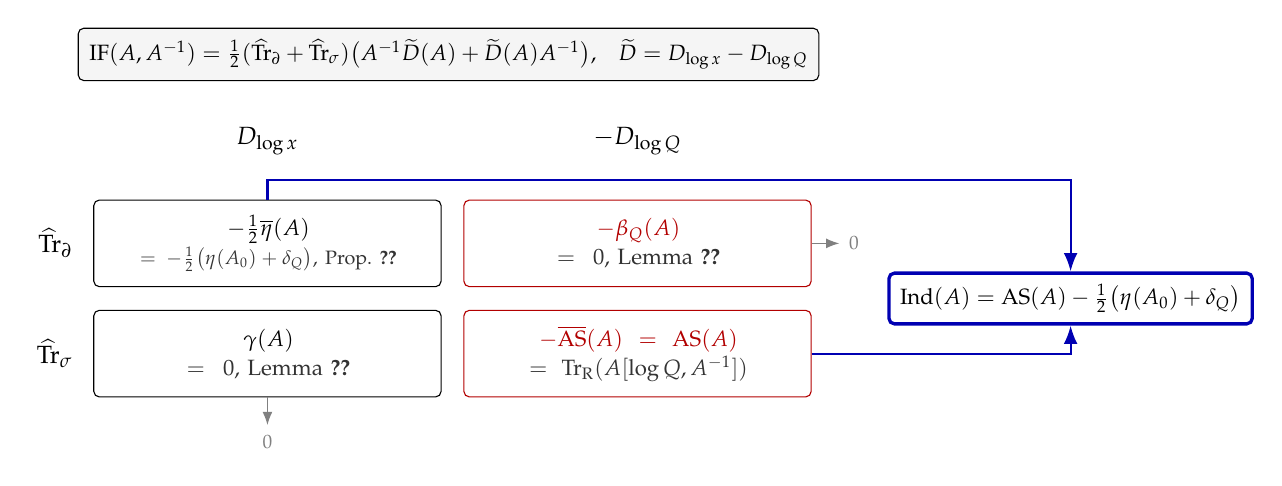
\begin{tikzpicture}[>=Latex,font=\footnotesize,
  cell/.style={draw,rounded corners=2pt,align=center,text width=4.2cm,
    minimum height=11mm,inner sep=3pt}]
 \node[draw,rounded corners=2pt,fill=gray!8,inner sep=4pt] (top) at (3.3,2.6)
   {\(\IF(A,A^{-1})=\tfrac12(\hTrd+\hTrs)\bigl(A^{-1}\widetilde D(A)+
    \widetilde D(A)A^{-1}\bigr)\),\quad \(\widetilde D=D_{\lx}-D_{\lQ}\)};
 \node[font=\small] at (1.0,1.5) {\(D_{\lx}\)};
 \node[font=\small] at (5.7,1.5) {\(-D_{\lQ}\)};
 \node[font=\small,anchor=east] at (-1.35,0.2) {\(\hTrd\)};
 \node[font=\small,anchor=east] at (-1.35,-1.2) {\(\hTrs\)};
 \node[cell] (dx) at (1.0,0.2) {\(-\tfrac12\etab(A)\)\\[1pt]
   {\scriptsize\color{gray!40!black}\(=-\tfrac12\bigl(\eta(A_0)+\delta_Q\bigr)\), Prop.~\ref{prop:eta}}};
 \node[cell,draw=red!70!black] (dq) at (5.7,0.2) {{\color{red!70!black}\(-\beta_Q(A)\)}\\[1pt]
   {\color{gray!40!black}\(=0\), Lemma~\ref{lem:betaQ}}};
 \node[cell] (sx) at (1.0,-1.2) {\(\gamma(A)\)\\[1pt]
   {\color{gray!40!black}\(=0\), Lemma~\ref{lem:gamma}}};
 \node[cell,draw=red!70!black] (sq) at (5.7,-1.2) {{\color{red!70!black}\(-\bAS(A)=\AS(A)\)}\\[1pt]
   {\color{gray!40!black}\(=\TrR(A[\lQ,A^{-1}])\)}};
 \node[draw,very thick,blue!70!black,rounded corners=2pt,inner sep=4pt,text=black]
   (ind) at (11.2,-0.5) {\(\Ind(A)=\AS(A)-\tfrac12\bigl(\eta(A_0)+\delta_Q\bigr)\)};
 \draw[->,thick,blue!70!black] (dx.north) -- (1.0,1.0) -| (ind.north);
 \draw[->,thick,blue!70!black] (sq.east) -| (ind.south);
 \draw[->,gray] (dq.east) -- ++(0.35,0) node[right,font=\scriptsize] {\(0\)};
 \draw[->,gray] (sx.south) -- ++(0,-0.35) node[below,font=\scriptsize] {\(0\)};
\end{tikzpicture}
\caption[Assembling the index formula]{The four terms of
Theorem~\ref{thm:index}. Inserting \(B=A^{-1}\) in
Proposition~\ref{prop:IF} and splitting \(\widetilde D=D_{\lx}-D_{\lQ}\)
gives one term for each pair of a regularized trace and a derivation:
\(\Ind(A)=-\bAS(A)-\frac12\etab(A)-\beta_Q(A)+\gamma(A)\). The terms in
red carry the signs corrected from \cite[(93)]{MN}
(Correction~\ref{corr:ASsign}). For \(A\) fully elliptic and translation
invariant near the boundary with normal indicial family, and \(Q\) as in
Theorem~\ref{thm:reduced}, the grey annotations apply: \(\gamma\) and
\(\beta_Q\) vanish, \(\etab\) is the eta invariant of \(A_0\) plus the
local correction \(\delta_Q\) coming from \cite[Prop.~8]{MN}
(item~\ref{item:Prop8reg} of Section~\ref{subsec:errata}), and the result
is the reduced formula. In the examples of Section~\ref{sec:examples},
\(\delta_Q=0\).}
\label{fig:fourterms}
\end{figure}

\subsection{The eta term}

\begin{proposition}[MN Proposition 17, corrected]\label{prop:eta}
Let \(A\in\Psic^m(X;E)\) be fully elliptic, and let \(Q\) be translation
invariant to all orders at \(\partial X\), with Taylor series \(Q_0^{-s}\)
at the front face. Let \(A_0=\In(A)\in\Psis^m(\partial X;E)\) and
\(t=1/x\). Then
\[
 \etab(A)=\eta(A_0)+\delta_Q(A),\qquad
 \eta(A_0)=2\,\bTr\bigl(A_0^{-1}[t,A_0]\bigr)=\frac1{\pi i}\,
 \overline{\int_{\R}}\Tr\bigl(A_0(\tau)^{-1}\partial_\tau A_0(\tau)\bigr)
 d\tau ,
\]
where \(\eta(A_0)\) is Melrose's eta invariant of \cite{MelroseEta}, (B7),
and \(\delta_Q(A)=(2\pi)^{-1}\gamma'(0)\), with \(\gamma\) the correction
of Proposition~\ref{prop:Tr8} computed from \(A_0^{-1}[t,A_0]Q_0^{-s}\)
and \([t,A_0]A_0^{-1}Q_0^{-s}\). The term \(\delta_Q(A)\) is a local
functional of the boundary symbols of \(A\) and \(Q\). It vanishes:
\begin{enumerate}
\item when the terms of homogeneity \(-n-s\) of these two symbols are odd
in \(\tau\); in particular when \(\partial X\) is a point and \(Q_0^{-s}\)
is even in \(\tau\) (Example~\ref{ex:interval-index});
\item when \(n\) is odd, \(A\) is a differential operator, and \(Q_0^{-s}\)
has parity type \(+1\), e.g.\ complex powers of a differential operator or
the family of Proposition~\ref{tr:prop:Q} (Remark~\ref{tr:rem:parity}, a
sketch). The parity hypothesis on \(Q\) is needed: for \(n=1\),
\(A=\partial_t+a\) and \(Q\) with indicial symbol
\(\langle\tau\rangle+\tau/2\) one finds \(\delta_Q=i\log3/\pi\neq0\) at
that end;
\item when \(A_0=\sigma(i\tau+B_\partial)\) is in APS normal form and
\(Q_0^{-s}=(D_t^2+B_\partial^2)^{-s/2}\) (Proposition~\ref{tr:prop:etabar}(ii));
\item when \(A\) is a Dirac operator compatible with a Clifford structure
and \(Q=(A^*A+1)^{1/2}\) (Remark~\ref{tr:rem:plusone}, quoting
Bismut--Freed \cite{BismutFreed}).
\end{enumerate}
\end{proposition}

\begin{proof}
This is Proposition~\ref{tr:prop:etabar}(i). In outline: a parametrix
\(B\in\Psic^{-m}\) has \(\In(B)=A_0^{-1}\). By
Lemma~\ref{lem:twist}(3), \([\lx,A]\in x\Psic^{m-1}\) with
\(\In(x^{-1}[\lx,A])=-[t,A_0]\) \cite[(95)]{MN}. Since \(x\) commutes with
everything to leading order, the coefficient of \(x^1\) in \(B[\lx,A]\) is
\(-C_1\), \(C_1=A_0^{-1}[t,A_0]\), and in \([\lx,A]B\) it is \(-C_2\),
\(C_2=[t,A_0]A_0^{-1}\). By the corrected Corollary~\ref{cor:Tr61}(2),
\[
 \etab(A)=\bTr(C_1)+\bTr(C_2)+\frac{\gamma_{C_1}'(0)+\gamma_{C_2}'(0)}{2\pi},
\]
and \(\bTr(C_2)=\bTr(C_1)\) because \(\bTr\) is a trace on \(\Psis^{\Z}\)
(Theorem~\ref{tr:thm:bTr}). By \eqref{eq:Inkernel},
\(\In([t,A_0])=-i\partial_\tau A_0\), so \(2\bTr(C_1)=2(2\pi)^{-1}
\overline\int\Tr(A_0^{-1}(-i)\partial_\tau A_0)\,d\tau\), which is the
second expression for \(\eta(A_0)\). For (1): \(\gamma(s)\) is the sum of
the values at \(\tau=+1\) and \(\tau=-1\) of the fibre integrals of the
terms of homogeneity \(-n-s\), which cancel for odd terms. If
\(\partial X\) is a point, that term of \(C_jQ_0^{-s}\) is the product of
the principal symbols, \(-im\tau^{-1}\) times that of \(Q_0^{-s}\), since
\(C_j=-iA_0^{-1}\partial_\tau A_0\) up to order; it is odd when
\(Q_0^{-s}\) is even. For (2)--(4) see the cited results.
\end{proof}

\begin{correction}[The proof of MN Proposition 17]\label{corr:eta}
The proof in \cite{MN} correctly obtains
\(\hTrd(B[\lx,A])=-\bTr(A_0^{-1}[t,A_0])=\hTrd([\lx,A]B)\), up to the local
correction of Corollary~\ref{cor:Tr61}(2), but then
concludes \(\etab(A)=-\bTr(A_0^{-1}[t,A_0])\). With definition
\cite[(89)]{MN} the conclusion is \(2\bTr(A_0^{-1}[t,A_0])+\delta_Q(A)\), in
agreement with \cite[(24)]{MN} when \(\delta_Q=0\); there \([\lx,A_0]\)
should read \([t,A_0]\). Also,
the proof cites \cite[(54)]{MN}; what is needed is \cite[Cor.~2]{MN},
in its corrected form, which assumes that \(Q\) is translation invariant to
all orders at the boundary. For
general \(Q\), Lemma~\ref{lem:hTrdQ} gives
\(\etab(A;Q)=\eta(A_0)+\delta_{Q_{\mathrm{ti}}}(A)+\Trds\bigl((A^{-1}[\lx,A]
+[\lx,A]A^{-1})\log(Q/Q_{\mathrm{ti}})\bigr)\), with \(Q_{\mathrm{ti}}\)
translation invariant to all orders. The corrections are compensated by
\(\beta_Q\), since the index does not depend on \(Q\).
\end{correction}

\begin{corollary}[MN Corollary 3]\label{cor:Dirac}
Suppose that near the boundary \(A=\sigma(-\partial_t+B_\partial)\), with
\(\sigma\) a unitary bundle map and \(B_\partial\) a self-adjoint first-order
elliptic differential operator on \(\partial X\) with
\(0\notin\operatorname{spec}B_\partial\). This is the
APS normal form \(\sigma(\partial_u+B_\partial)\) in the inward normal
variable \(u=-t\). Then \(\eta(A_0)=\eta_{\mathrm{APS}}(B_\partial)=
\sum_\lambda\sgn\lambda\) (regularized). If \(Q\) is as in
Proposition~\ref{prop:eta}(3) or~(4), then also \(\etab(A)=
\eta_{\mathrm{APS}}(B_\partial)\).
\end{corollary}

\begin{proof}
\(\In(A,\tau)=e^{i\tau t}Ae^{-i\tau t}=\sigma(i\tau+B_\partial)\). Formally,
on the \(\lambda\)-eigenspace
\(\Tr(A_0^{-1}\partial_\tau A_0)=i/(\lambda+i\tau)=(i\lambda+\tau)/
(\lambda^2+\tau^2)\); the odd part integrates to zero over \([-T,T]\), and
\((\pi i)^{-1}\int i\lambda/(\lambda^2+\tau^2)\,d\tau=\sgn\lambda\). The
proof that the regularized sum is \(\eta_{B_\partial}(0)\) is
Theorem~\ref{tr:thm:Dirac}. The last statement is
Proposition~\ref{prop:eta}(3),(4).
\end{proof}

\subsection{Simplifications}

\begin{lemma}[MN Lemma 15]\label{lem:gamma}
Let \(A\in\Psic^m(X;E)\) be fully elliptic and translation invariant in a
collar \(\{x'<\epsilon\}\) with respect to a normal fibration. Choose
\(x=f(x')\) with \(f(x')=x'\) near \(0\) and \(x\equiv1\) outside
\(\{x'<\epsilon\}\). Then \(\gamma(A)=0\).
\end{lemma}

\begin{proof}
In the collar write \(\log x=G(t')\) with \(t'=1/x'\). So
\(G(t')=-\log t'\) for large \(t'\), and \(G\) is constant (\(=0\)) near
\(t'=1/\epsilon\). For translation invariant \(A\), Taylor expansion of
\(G(t)-G(t')\) about the diagonal gives
\[
 [\lx,A]\sim\sum_{j\ge1}G^{(j)}(t')R_j ,
\]
with \(R_j\) translation invariant of order \(m-j\) \cite[p.~32]{MN}. The
same holds for \(B[\lx,A]\) and \([\lx,A]B\), with other translation
invariant coefficients \(R_j'\), since a parametrix \(B\) can also be
taken translation invariant there. The residue density of
\(G^{(j)}(t')R_j'\) is \(G^{(j)}(t')\) times the constant residue density
of \(R_j'\). By \eqref{eq:55}, \(\hTrs\) integrates it against
\(dt'\nu_\partial\) and takes the Hadamard finite part as \(x\to0\). For
\(j\ge2\), \(\int G^{(j)}dt'=[G^{(j-1)}]\) vanishes at both ends, since
\(G^{(j-1)}=O(t'^{1-j})\) at infinity and \(G\) is constant at the inner
end. For \(j=1\), \(\int_{1/\epsilon}^{T}G'\,dt'=G(T)-G(1/\epsilon)=
\log x|_{x=1/T}-0\), which is purely logarithmic and is removed by the
finite part. Outside the collar \(d\log x=0\), so there is no further
contribution.
\end{proof}

\begin{lemma}[MN Lemma 16]\label{lem:betaQ}
Suppose that \(A\in\Psic^m(X;E)\), \(m>0\), is fully elliptic and normal to
first order at the boundary: \([A^*,A]\in x^2\Psic^{2m-1}(X;E)\). Let
\(Q=(A^*A+1)^{1/2m}\). Then \([\lQ,A]\in x^2\Psic^{m-1}\), so
\(\beta_Q(A)=0\), and the integral defining \(\bAS(A)\) converges without
regularization.
\end{lemma}

\begin{proof}
\([A,A^*A]=[A,A^*]A\in x^2\Psic^{3m-1}\), so by the functional calculus
\(A\) commutes with functions of \(A^*A\) modulo \(x^2\). Hence
\([\lQ,A]\in x^2\Psic^{m-1}\). The functional \(\hTrd\) only sees the
coefficient of \(x^1\): for \(C\in x^2\Psic\) the function \(Z(C;s,z)\)
has no pole at \(z=0\), since its poles lie at \(z=-1-j\). So
\(\beta_Q(A)=0\). Similarly \(\Trs(x^zC)\) is regular at \(z=0\) for
\(C\in x^2\Psic\), so no finite part is needed in \eqref{eq:55}. For
operators of order \(\le0\), replace \(1\) by an operator that is positive
in the interior and vanishes near the boundary \cite[p.~33]{MN}.
\end{proof}

\begin{theorem}[Reduced index theorem, MN (99)--(100), corrected]
\label{thm:reduced}
Let \(A\in\Psic^m(X;E)\) be fully elliptic and translation invariant near
the boundary, with normal indicial family \(A_0\). Let \(Q=(A^*A+1)^{1/2m}\); it is positive,
translation invariant near the boundary and commutes with \(A\) there.
(The proof uses Lemma~\ref{lem:betaQ}, which is specific to this \(Q\).)
Then
\begin{gather*}
 \Ind(A)=\AS(A)-\tfrac12\bigl(\eta(A_0)+\delta_Q(A)\bigr),\\
 \AS(A)=\TrR\bigl(A[\lQ,A^{-1}]\bigr)=-\TrR\bigl(A^{-1}[\lQ,A]\bigr),
\end{gather*}
where the residue integral converges, and \(\eta(A_0)\) and the local
correction \(\delta_Q(A)\) are as in Proposition~\ref{prop:eta}. In
particular \(\Ind(A)=\AS(A)-\frac12\eta(A_0)\) whenever \(\delta_Q(A)=0\),
for instance in the cases (1)--(4) of Proposition~\ref{prop:eta}.
\cite[(99)--(100)]{MN} state the formula without \(\delta_Q\).
\end{theorem}

\begin{proof}
By Lemmas~\ref{lem:gamma} and~\ref{lem:betaQ}, \(\gamma=\beta_Q=0\), and
by Proposition~\ref{prop:eta}, \(\etab(A)=\eta(A_0)+\delta_Q(A)\). The two terms of
\(\AS\) agree, because \(\hTrs([C_1,C_2])=-\Trds(C_1[\lx,C_2])\) vanishes
for \(C_2=[\lQ,A]\in x^2\Psic\) (Lemma~\ref{lem:17}).
\end{proof}

\section{Worked examples of the index formula}\label{sec:examples}

\begin{example}[The closed circle]\label{ex:circle-index}
This is Section~\ref{subsec:circle}. With \(A=e^{i\theta}\Pi+(1-\Pi)\),
\(\Ind A=-1=\AS(A)\) and \(\bAS(A)=+1\). This fixes the sign of the
symbolic term.
\end{example}

\begin{figure}[htbp]
\centering
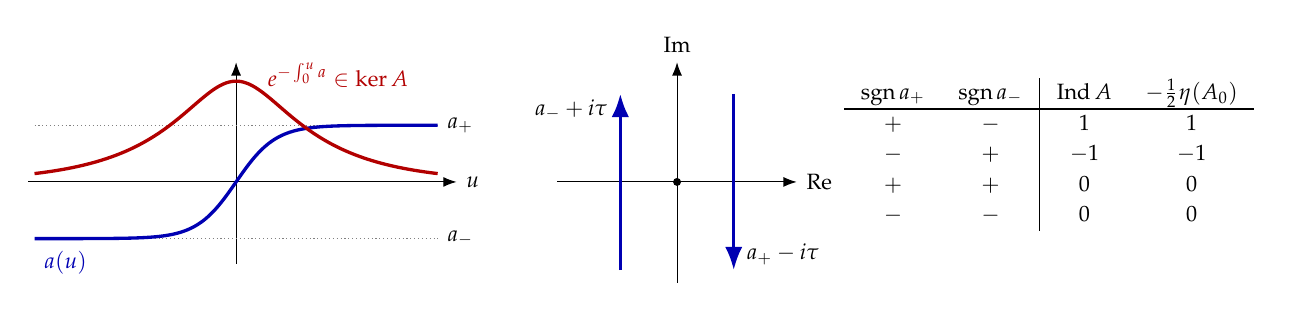
\begin{tikzpicture}[>=Latex,font=\footnotesize]
 \begin{scope}[scale=0.8]
  \draw[->] (-3.3,0)--(3.5,0) node[right] {\(u\)};
  \draw[->] (0,-1.3)--(0,1.9);
  \draw[gray,densely dotted] (-3.2,0.9)--(3.2,0.9) (-3.2,-0.9)--(3.2,-0.9);
  \node[anchor=west] at (3.2,0.9) {\(a_+\)};
  \node[anchor=west] at (3.2,-0.9) {\(a_-\)};
  \draw[very thick,blue!70!black,domain=-3.2:3.2,samples=80,smooth]
    plot (\x,{0.9*tanh(1.6*\x)});
  \draw[very thick,red!70!black,domain=-3.2:3.2,samples=80,smooth]
    plot (\x,{1.6*cosh(1.6*\x)^(-0.5625)});
  \node[blue!70!black,anchor=north west] at (-3.2,-0.95) {\(a(u)\)};
  \node[red!70!black,anchor=south west] at (0.35,1.35) {\(e^{-\int_0^ua}\in\ker A\)};
 \end{scope}
 \begin{scope}[xshift=5.6cm,scale=0.8]
  \draw[->] (-1.9,0)--(1.9,0) node[right] {\(\operatorname{Re}\)};
  \draw[->] (0,-1.6)--(0,1.9) node[above] {\(\operatorname{Im}\)};
  \fill (0,0) circle (1.8pt);
  \draw[very thick,blue!70!black,->] (0.9,1.4)--(0.9,-1.4);
  \draw[very thick,blue!70!black,->] (-0.9,-1.4)--(-0.9,1.4);
  \node[anchor=west,align=left] at (0.95,-1.15) {\(a_+-i\tau\)};
  \node[anchor=east,align=right] at (-0.95,1.15) {\(a_-+i\tau\)};
 \end{scope}
 \node[anchor=west] at (7.6,0.35) {%
  \renewcommand{\arraystretch}{1.15}%
  \begin{tabular}{cc|cc}
   \(\sgn a_+\) & \(\sgn a_-\) & \(\Ind A\) & \(-\tfrac12\eta(A_0)\)\\\hline
   \(+\) & \(-\) & \(1\) & \(1\)\\
   \(-\) & \(+\) & \(-1\) & \(-1\)\\
   \(+\) & \(+\) & \(0\) & \(0\)\\
   \(-\) & \(-\) & \(0\) & \(0\)
  \end{tabular}};
\end{tikzpicture}
\caption[The operator \(\partial_u+a(u)\) on the interval]{Example~\ref{ex:interval-index},
\(A=\partial_u+a(u)\) with \(a\) real and \(a=a_\pm\neq0\) near
\(u=\pm\infty\). Left: for \(a_+>0>a_-\) the solution \(e^{-\int_0^ua}\)
of \(Au=0\) decays at both ends, so \(\ker A\ne0\). Middle: the indicial
families \(a_+-i\tau\) (right end) and \(a_-+i\tau\) (left end) trace
vertical lines, which miss \(0\) because \(a_\pm\) are real and non-zero.
Right: since \(\AS(A)=0\), \(\delta_Q=0\) and the ends contribute
\(\eta=-\sgn a_+\) and \(\eta=\sgn a_-\), the formula
\(\Ind A=\AS(A)-\frac12\eta(A_0)\) gives
\(\tfrac12(\sgn a_+-\sgn a_-)\) in all four cases.}
\label{fig:interval}
\end{figure}

\begin{example}[First order operators on an interval]\label{ex:interval-index}
Let \(X\) be the compactification of \(\R_u\) at both ends by \(1/|u|\).
So \(X\cong[-1,1]\), \(n=1\), \(N=2\), and near the ends \(x=1/|u|\) and
\(t=|u|\). Let \(a\in\CI(\R;\R)\) be real-valued, with \(a(u)=a_\pm\) for
\(\pm u>R\) and \(a_\pm\neq0\), and consider
\[
 A=\partial_u+a(u)\in\Psic^1(X).
\]
\emph{Full ellipticity.} The principal symbol is \(i\xi\ne0\). At the right
end \(t=u\), so \(A=\partial_t+a_+\) and \(\In(A,\tau)=e^{i\tau t}(\partial_t
+a_+)e^{-i\tau t}=a_+-i\tau\). At the left end \(t=-u\), so
\(A=-\partial_t+a_-\) and \(\In(A,\tau)=a_-+i\tau\). Since \(a_\pm\) are
real and non-zero, both are invertible for all real \(\tau\). (For complex
\(a_\pm\) this fails: \(a_+=i\) gives \(a_+-i\tau=0\) at \(\tau=1\). Reality
of \(a\) is also used below for the formal adjoint \(-\partial_u+a\).)

\emph{Index directly.} A solution of \(Au=0\) is a multiple of
\(\exp(-\int a)\). It lies in \(\dCI(X)\) (rapid decay as \(|u|\to\infty\))
if and only if \(a_+>0>a_-\). For the formal adjoint \(-\partial_u+a\), the
condition is \(a_+<0<a_-\). Hence
\[
 \Ind A=\tfrac12\bigl(\sgn a_+-\sgn a_-\bigr).
\]
Figure~\ref{fig:interval} shows the case \(a_+>0>a_-\) and the four sign
cases.
\emph{The formula.} Take \(Q=(A^*A+1)^{1/2}\). Near the ends
\(A^*A=-\partial_u^2+a_\pm^2\) commutes with \(A\), so \(A\) is normal
there and Theorem~\ref{thm:reduced} applies. The symbol of \([\lQ,A]\) is
\(-i\{\log\langle\xi\rangle+c_{-1}+\cdots,\,i\xi+a\}\), of order \(-1\),
because the principal symbol \(i\xi\) of \(A\) does not depend on \(u\).
So \(A^{-1}[\lQ,A]\) has order \(-2\), and its residue density
(homogeneity \(-n=-1\)) vanishes: \(\AS(A)=0\).

\emph{The correction \(\delta_Q\) vanishes.} Here \(\partial X\) consists
of two points, so \(d=0\), and near each end \(Q_0^{-s}=(\tau^2+a_\pm^2+
1)^{-s/2}\) is even in \(\tau\). At the right end \(C_1=C_2=
A_0^{-1}[t,A_0]=-(a_+-i\tau)^{-1}=-(a_++i\tau)/(a_+^2+\tau^2)\), whose
expansion begins with \(-i\tau^{-1}\). The term of homogeneity \(-1-s\) of
\(C_1Q_0^{-s}\) is therefore \(-i\tau^{-1}|\tau|^{-s}\), which is odd in
\(\tau\): its values at \(\tau=\pm1\) cancel, so \(\gamma(s)\equiv0\) in
Proposition~\ref{prop:Tr8} (Theorem~\ref{tr:thm:susreg}). The left end is
the same, with \(C_1=(a_-+i\tau)^{-1}\). Hence \(\delta_Q(A)=0\) exactly,
by case (1) of Proposition~\ref{prop:eta} (this is also an instance of the
parity statement (2), with \(n=1\), but the computation here is complete),
and \(\etab(A)=\eta(A_0)\). By Proposition~\ref{prop:eta}, at the right
end
\[
 \eta=\frac1{\pi i}\int\frac{-i}{a_+-i\tau}\,d\tau=-\frac1\pi\int
 \frac{a_++i\tau}{a_+^2+\tau^2}\,d\tau=-\sgn a_+ ,
\]
and at the left end \(\eta=\frac1{\pi i}\int\frac{i}{a_-+i\tau}d\tau=
\sgn a_-\). So
\[
 \AS(A)-\tfrac12\eta(A_0)=0-\tfrac12\bigl(-\sgn a_++\sgn a_-\bigr)
 =\tfrac12\bigl(\sgn a_+-\sgn a_-\bigr)=\Ind A .
\]
This confirms the sign of the eta term in \cite[(93)]{MN} and the sign of
\(\widetilde D\) in Proposition~\ref{prop:IF}. If instead \(\widetilde D\)
had the sign of \cite[(21)]{MN}, the eta term would enter with \(+\frac12\)
and the formula would give \(-\Ind A\). At the right end the boundary
operator in APS form is \(B_\partial=-a_+\) (Corollary~\ref{cor:Dirac}),
and \(\eta_{\mathrm{APS}}(B_\partial)=-\sgn a_+\), as found.
\end{example}

\begin{example}[Dirac operators on manifolds with cylindrical ends]
Let \(\eth\) be a Dirac operator for an exact cusp metric
(Remark~\ref{rem:cuspmetric}) and a product structure near the boundary,
\(\eth=\sigma(-\partial_t+\eth_\partial)\). If \(\eth_\partial\) is
invertible, \(\eth\) is fully elliptic. In the \(\mathbb Z_2\)-graded
setting of Section~\ref{subsec:graded}, Theorem~\ref{thm:reduced} and
Corollary~\ref{cor:Dirac} give
\[
 \Ind\eth^+=\AS(\eth)+\nu-\tfrac12\eta(\eth_\partial),
\]
where \(\nu\) is the interior correction of \cite[(110)]{MN}. Here we take
\(Q=(\eth^*\eth+1)^{1/2}\); the correction \(\delta_Q\) of
Proposition~\ref{prop:eta} vanishes by Remark~\ref{tr:rem:plusone}, which
quotes the local cancellation of Bismut--Freed \cite{BismutFreed}. For a
general first-order \(\eth_\partial\) a local term
\(-\frac12\delta_Q\) would remain. This is the
APS theorem in the invertible case. The term
\(\AS\) is the residue form of the Atiyah--Singer integrand, by the
local index theorem. MN do not evaluate it further.
\end{example}

\section{Cyclic homology, the graded case and other algebras (MN \S\S13--15)}
\label{sec:other}

We summarize the remaining sections of \cite{MN}, with comments.

\subsection{Cyclic homology}
For a unital algebra the Connes--Loday--Quillen sequence
\(\cdots\to\HH_n\xrightarrow{I}\HC_n\xrightarrow{S}\HC_{n-2}
\xrightarrow{B}\HH_{n-1}\to\cdots\) relates cyclic and Hochschild homology
\cite[(101)--(103)]{MN}. The key point is \cite[Lemma~17]{MN}: \(B=0\) for
\(\As\), \(\Is\), \(\Ads\), \(\Id\). The reason is an order count. By the
spectral sequences, \(\HH_q\) is generated by cycles of order \(q-n\)
(\(x\)-degree for \(\Id\)), and all cycles of lower order are
boundaries. Inductively \(\HC_{m-1}\cong\bigoplus_k\HH_{m-1-2k}\) is
generated by elements of order at most \(m-1-n\). The operator \(B\) does
not raise order, so it maps them into cycles of order less than \(m-n\),
which are boundaries. Hence \cite[Prop.~18]{MN}
\[
 \HC_m(\mathfrak A)\cong\bigoplus_{k\ge0}\HH_{m-2k}(\mathfrak A),\qquad
 \mathfrak A=\As,\Is,\Ads,\Id,\Ad ,
\]
with \(S\) the projection, and periodic cyclic homology obtained by
dropping the restriction \(k\ge0\). For \(\Ad\) MN write
\(\HC_i(\Ad)\cong\HC_i(\Ads)/\C\) for \(i>0\). With
Proposition~\ref{prop:Ad}, the codimension is \(N\) in general, and the
statement is about dimensions: in homology \(\HH_{1,2}(\Ad)\) are
subspaces of \(\HH_{1,2}(\Ads)\), not quotients.

\subsection{Bundles and grading}\label{subsec:graded}
Dirac operators map between different bundles \(E^\pm\). MN therefore
pass to \(\mathbb Z_2\)-graded algebras \cite[\S14]{MN}. A graded embedding
\(E\subset X\times(\C^N\oplus\C^N)\) gives a graded HKR map with the
supertrace and the Grassmann connection \cite[(105)]{MN}. The Hochschild
groups have the same dimensions as in the ungraded case and do not depend
on the embedding \cite[Lemma~18, Prop.~19]{MN}. If \(E^+=E^-\) near the
boundary, the index of an odd fully elliptic \(A\) is
\cite[Thm.~1, (111)]{MN}
\[
 \Ind(A)=\IF([A],[A]^{-1})+\nu,\qquad
 \nu=\Tr\bigl(e^+Q_N^{-s}\bigr)-\Tr\bigl(e^-Q_N^{-s}\bigr)\big|_{s=0},
\]
a local interior correction coming from the embedding. Proposition~\ref{prop:IF}
holds verbatim, and so do our sign corrections.

\subsection{Other algebras}\label{subsec:other}
The method applies to \(\Psic^{\Z}(X)\), \(\Psic^0(X)\), complete symbol
algebras and the b-calculus, but the groups can be infinite dimensional
\cite[\S15]{MN}. For \(\mathcal A_6=x^{-\Z}\Psic^0(X)/x^{-\Z}\Psic^{-\infty}
(X)\) the \(E^1\) term agrees with that of \(\Ads\) for \(p\le0\) and
vanishes for \(p>0\). The \(E^2\) term is unchanged for \(p<0\), while
\(E^2_{0,q}\) consists of spaces of closed forms \cite[Prop.~20]{MN}. This
is the precise sense in which restricting to order zero destroys
finiteness. (MN state the \(E^1\) comparison with \(\Ads\). Since
\(\mathcal A_6\) is the order-\(\le0\) part of \(\As\), and the stated
\(E^2_{0,q}\) involves forms on \(Y\) as well as on \(Z\), this is
presumably a misprint for \(\As\).)

\section{Comparison with the b-calculus}\label{sec:comparison}

The companion notes \cite{HHb} carry out the b-calculus analogue of
\cite{MN}, as MN suggest \cite[p.~3]{MN}. Table~\ref{tab:compare}
summarizes the differences.

\begin{table}[htbp]
\centering
\renewcommand{\arraystretch}{1.3}
\begin{tabular}{p{3.6cm}p{5.2cm}p{5.2cm}}
 & cusp calculus \cite{MN} & b-calculus \cite{HHb}\\\hline
 vector fields & \(x^2\partial_x,\ \partial_y\) & \(x\partial_x,\ \partial_y\)\\
 boundary variable & \(t=1/x\), translations & \(\log x\), dilations\\
 indicial family & \(\In(A,\tau)\), \(\tau\in\R\), symbol class & \(I(A,\lambda)\),
 entire in \(\lambda\in\C\)\\
 conjugation by \(x\) & \(x^{-1}Ax=A+O(x)\): a \emph{derivation} at leading
 order, \([x,\partial_t]=x^2\) & \(I(x^{-1}Ax,\lambda)=I(A,\lambda-i)\): an
 \emph{automorphism}\\
 graded algebra of \(\Id\) & commutative, Poisson & skew Laurent series\\
 method for \(\Id\) & \(x\)-adic spectral sequence & weight decomposition,
 crossed products\\
 invertibility in \(\cA\) & \(\In(A,\tau)\) invertible for \(\tau\in\R\) &
 \(I(A,\lambda)\) invertible for all \(\lambda\in\C\)\\
 \(\HH^{0,1}(\Id)\) & \(\C^N\), \(\C^N\) & \(\C^N\), \(\C^N\)\\
 rank of \(\HH^1(\Id)\to\HH^2(\As)\) & \(N-1\) (MN: \(0\)) & \(N-1\)\\
 trace defect on \(\Id\) & \(b\Tr_c=-i_{\lx}\Trd\) & b-trace defect
 formula\\
\end{tabular}
\caption{Cusp versus b-calculus.}
\label{tab:compare}
\end{table}

\subsection{Derivation twist versus automorphism twist}
In the cusp calculus, Lemma~\ref{lem:twist} shows that commuting \(x\) past
an indicial operator produces terms of \emph{higher} order in \(x\),
governed by the derivation \(\partial_\tau\). The associated graded
algebra is therefore commutative, with Poisson bracket \(\{t,\tau\}=1\).
The \(x\)-adic spectral sequence is then a Brylinski--Getzler computation on
\(\R_\tau\times\Sd\) (Proposition~\ref{prop:Idpoint}). In the b-calculus,
\(x^{-1}Ax\) has indicial family \(I(A,\lambda-i)\). The complex shift by
\(-i\) is an automorphism that is \emph{not} close to the identity, so the
associated graded algebra is a skew Laurent series ring. The
computation proceeds by a weight decomposition and the homology of crossed
products by \(\Z\) \cite[\S``The boundary ideal'']{HHb}. The answers agree,
\(\HH_{0,1}(\Id)\cong\C^N\). The generators are also closely related:
\(\Trd\) and \(i_{\lx}\Trd\) in the cusp case, and the boundary trace
\(\Tr_\partial\) and the cocycle \(\varphi\) of \cite{HHb} in the b-case.

\subsection{Several boundary components}
In both calculi the boundary algebras are direct sums over components,
and the only global interaction is through the interior symbol algebra.
The map \(\HH^1(\Id)\to\HH^2(\As)\) sends \(i_{\lx}\Tr_{\partial,j}\) to
the de Rham coboundary of \(d\theta_\sigma1_{Z_j}\)
(Proposition~\ref{prop:HHA}). Its kernel is spanned by the sum over \(j\),
because only \(\sum_j1_{Z_j}=1_Z\) extends over the connected \(Y\).
Equivalently, by Stokes' theorem, \(\sum_j\int_{Z_j}\beta=0\) for every
closed \(\beta\) on \(Y\). This is the rank \(N-1\) phenomenon of
\cite[Remark ``Several boundary components'']{HHb}. In the cusp case MN's
argument (``\(d\theta_\sigma\) extends'') covers only the sum, and their
statements (16) and Proposition~12 are correct exactly when \(N=1\).
Proposition~\ref{prop:I} shows the same rank in the simplest setting:
\(\HH_1(x^{-\Z}\Psic^{-\infty}(X))\cong\C^{N-1}\), the cusp analogue of
\cite[Thm., part (iii)]{HHb}.

\subsection{Invertibility, completeness and the trace defects}

\begin{figure}[htbp]
\centering
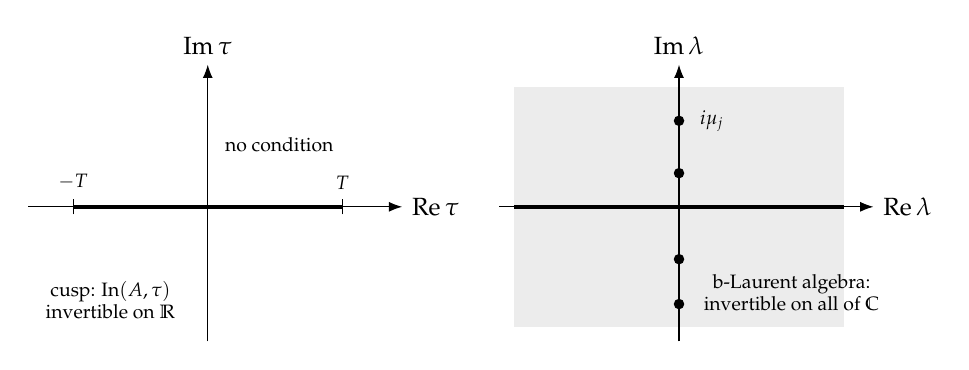
\begin{tikzpicture}[>=Latex,scale=0.95]
 \begin{scope}
  \draw[->] (-2.4,0)--(2.6,0) node[right] {\small \(\operatorname{Re}\tau\)};
  \draw[->] (0,-1.8)--(0,1.9) node[above] {\small \(\operatorname{Im}\tau\)};
  \draw[line width=1.6pt] (-1.8,0)--(1.8,0);
  \draw (-1.8,-0.1)--(-1.8,0.1) node[above,font=\scriptsize] {\(-T\)};
  \draw (1.8,-0.1)--(1.8,0.1) node[above,font=\scriptsize] {\(T\)};
  \node[font=\scriptsize,align=center] at (-1.3,-1.25) {cusp: \(\In(A,\tau)\)\\ invertible on \(\R\)};
  \node[font=\scriptsize,anchor=south west] at (0.1,0.6) {no condition};
 \end{scope}
 \begin{scope}[xshift=6.3cm]
  \fill[gray!15] (-2.2,-1.6) rectangle (2.2,1.6);
  \draw[->] (-2.4,0)--(2.6,0) node[right] {\small \(\operatorname{Re}\lambda\)};
  \draw[->] (0,-1.8)--(0,1.9) node[above] {\small \(\operatorname{Im}\lambda\)};
  \draw[line width=1.6pt] (-2.2,0)--(2.2,0);
  \foreach \m in {-1.3,-0.7,0.45,1.15} \fill (0,\m) circle (2pt);
  \node[font=\scriptsize,anchor=west] at (0.15,1.15) {\(i\mu_j\)};
  \node[font=\scriptsize,align=center,anchor=west] at (0.2,-1.15) {b-Laurent algebra:\\ invertible on all of \(\C\)};
 \end{scope}
\end{tikzpicture}
\caption[Where indicial families must be invertible]{Left: a cusp
operator is fully elliptic when \(\In(A,\tau)\) is invertible for real
\(\tau\) (thick line). The eta term is the regularized integral of
\(\Tr(A_0^{-1}\partial_\tau A_0)\) over \([-T,T]\), with
\(T\to\infty\) by Hadamard's finite part. Right: in the b-calculus
\(I(A,\lambda)\) is entire, and invertibility in the b-Laurent algebra
requires \(I(A,\lambda)\) to be invertible on all of \(\C\) (shaded). A
Dirac operator \(x\partial_x+B_\partial\) has indicial roots \(i\mu_j\),
\(\mu_j\in\operatorname{spec}B_\partial\) (dots), so it is never invertible
there. Fredholmness on \(L^2_b\) needs only the real axis, which is
exactly the cusp condition after the transcendental blow-up.}
\label{fig:contour}
\end{figure}

In the b-calculus, invertibility in \(\cA_b\) forces the indicial family
to be invertible on all of \(\C\) (Section~\ref{subsec:transcendental}).
Dirac operators never satisfy this, so the b-Laurent algebra cannot see
APS-type indices. The cusp calculus needs invertibility only on \(\R\),
which is the APS condition \(\ker B_\partial=0\). Under the transcendental
blow-up \(x_b=e^{-1/x}\) the b-indicial family becomes the cusp indicial
family with \(\tau=\lambda\). A b-operator with indicial family invertible
on \(\R\) lifts to a fully elliptic cusp operator, and its index is given
by Theorem~\ref{thm:index}. The trace defects also match. For translation
invariant \(A,B\), Proposition~\ref{prop:Idpoint} and
Proposition~\ref{prop:I} give
\[
 \Tr_c([A,B])=-\Trd(A[\lx,B])=-\frac i{2\pi}\int_{\R}\Tr\bigl(\In(A,\tau)\,
 \partial_\tau\In(B,\tau)\bigr)\,d\tau .
\]
The b-trace satisfies the same identity in the variable \(\lambda\):
\({}^b\Tr([A,B])=-\Res_z\Tr(A[\log x_b,B]x_b^z)\), and
\(I([\log x_b,B])=i\partial_\lambda I(B)\) \cite[Lemma ``Conjugation by
powers of \(x\)'']{HHb}. This is Melrose's b-trace defect formula. The
two regularizations differ (\(x^z\) versus \(x_b^z=e^{-z/x}\)), but on the
leading terms they agree.

\appendix
% The parts are found both when compiling from "Lecture draft/" and when
% latexmk runs from the repository root (see the Makefile target mn).
\makeatletter
\providecommand*\input@path{}
\g@addto@macro\input@path{{Lecture draft/}}
\makeatother
\section{Construction of the cusp calculus}\label{cc:sec:cusp}
\providecommand{\ccK}{\mathfrak K}
\providecommand{\Psiu}{\Psi_{\mathrm u}}
\providecommand{\PsicT}{\Psi_{c,T}}
\providecommand{\ccM}{\mathcal M}
\providecommand{\ffc}{\mathrm{ff}_c}
\providecommand{\ffb}{\mathrm{ff}_b}
\providecommand{\adt}{\operatorname{ad}_t}
\providecommand{\CIb}{C^\infty_{\mathrm b}}
\providecommand{\ccS}{S_{\mathrm{cl}}}

This appendix proves the background facts (B1) and (B2) of
Section~\ref{subsec:background}, as they are stated there. We construct
the cusp calculus, prove that it is a doubly filtered algebra, and derive
the symbol sequence \cite[(11)]{MN}, the indicial sequence
\cite[(12)]{MN}, the global quantization \cite[Prop.~24]{MN}, the Taylor
series isomorphism \cite[Prop.~25]{MN} and the invariance of orders under
conjugation by \(x^z\). We then prove the Fredholm theorem (B2).

\paragraph{What is proved and what is quoted.} We quote one thing: the
standard calculus of pseudodifferential operators on the cylinder
\(\R\times H\), \(H\) closed, with symbol estimates uniform in the
cylinder variable (Background fact~\ref{cc:bg:uniform}). This is a
boundaryless calculus. It is the calculus of \cite[Ch.~2]{MelroseMicro}
on \(\R^n\), transplanted to \(\R\times H\) by a partition of unity on
\(H\), and it contains nothing about cusps. Every statement that is
specific to the cusp calculus is proved here, except the density
statement in \cite[Prop.~26]{MN} (Remark~\ref{cc:rem:density}), which the
notes do not use.

\paragraph{Strategy.} The usual route to composition is the triple space
\cite{MazzeoMelrose}. We avoid it. Near the boundary a cusp operator is an
operator on the cylinder \(\R_t\times\partial X\), \(t=1/x\), whose kernel
is a smooth function of \(x=1/t\) with values in suspended kernels. We
show (Lemma~\ref{cc:lem:char}) that this smoothness is equivalent to
stability of the operator under the derivation \(\delta=t^2[\partial_t,
\cdot\,]\). The derivation obeys a Leibniz rule
(Lemma~\ref{cc:lem:identities}). Composition is then reduced to the
uniform calculus, with no new estimates.

\subsection{Conventions}\label{cc:subsec:conventions}
\(X\) is a compact manifold with boundary, of dimension \(n\), with a cusp
structure (Section~\ref{subsec:cuspstructure}) represented by the
boundary defining function \(x\). We fix a collar
\([0,\epsilon)_x\times\partial X\hookrightarrow X\) whose first coordinate
is \(x\) (a normal fibration). On the collar \(t=1/x\), so the collar is
the end \(\{t>1/\epsilon\}\) of the cylinder \(\R_t\times\partial X\). We
fix a smooth positive density \(\nu_\partial\) on \(\partial X\) and a cusp
density \(\nu_c\) on \(X\), smooth and positive in the interior and equal
to \(x^{-2}dx\,\nu_\partial=dt\,\nu_\partial\) on the collar. Operators are
identified with their kernels with respect to \(\nu_c\) in the second
variable:
\[
 Au(z)=\int_XK_A(z,z')u(z')\,\nu_c(z').
\]
\(\dCI(X)\) is the space of smooth functions vanishing to infinite order at
\(\partial X\), and \(\dCI(X^2)\) the space of smooth functions on \(X^2\)
vanishing to infinite order at \(\partial(X^2)\). Since \(x'^{-2}\) is a
smooth weight, a kernel lies in \(\dCI(X^2)\) with respect to \(\nu_c\) if
and only if it does with respect to a smooth density.

The cusp cotangent coordinates are \((x,y,\tau,\eta)\) as in
\eqref{eq:cuspcovector}. So \(\tau\) is the symbol of \(x^2D_x=-D_t\). If
\(\sigma\) denotes the covariable dual to \(t\), then \(\tau=-\sigma\).
Orders are integers, as in \cite{MN}. Nothing changes for real orders.

We write the proofs for scalar operators and connected \(\partial X\).
Several boundary components are handled one at a time. For bundles \(E\),
we trivialize \(E\) over the collar as the pull-back of
\(E|_{\partial X}\); kernels then take values in
\(\operatorname{Hom}(E)\), and every argument below applies entrywise.

\subsection{Background: conormal kernels and the uniform calculus on a
cylinder}\label{cc:subsec:background}
Let \(H\) be a closed manifold of dimension \(n-1\) with a smooth positive
density \(\nu_H\). In the application \(H=\partial X\).

\begin{definition}[Suspended kernels]\label{cc:def:K}
For \(m\in\Z\), \(\ccK^m(H)\) is the space of distributions \(\kappa\) on
\(\R_\mu\times H\times H\) such that
\begin{enumerate}
\item away from \(\{0\}\times\Delta_H\), \(\kappa\) is smooth, and for
every \(N\) and every derivative \(\partial^\alpha\) in \((\mu,y,y')\),
\(\langle\mu\rangle^N\partial^\alpha\kappa\) is bounded on
\(\{|\mu|\ge1\}\);
\item near each point of \(\{0\}\times\Delta_H\), in local coordinates
\(y\) on \(H\) and modulo a smooth function,
\begin{equation}\label{cc:eq:Kquant}
 \kappa(\mu,y,y')=(2\pi)^{-n}\int_{\R^n}e^{-i\mu\tau+i(y-y')\cdot\eta}\,
 a(y,\tau,\eta)\,d\tau\,d\eta ,
\end{equation}
with \(a\) a classical symbol of order \(m\) in \(\zeta=(\tau,\eta)\).
\end{enumerate}
The leading part of \(a\) is a well-defined function
\(\sigma_m(\kappa)\) on \((T^*H\times\R_\tau)\setminus0\), homogeneous of
degree \(m\): the principal symbol. We give \(\ccK^m(H)\) its usual Fr\'echet
topology and put \(\ccK^{-\infty}(H)=\bigcap_m\ccK^m(H)\).
\end{definition}

\begin{definition}[The suspended algebra]\label{cc:def:sus}
\(\Psis^m(H)\) is the space of operators on \(\R_t\times H\) given by
convolution in \(t\) with some \(\kappa\in\ccK^m(H)\):
\[
 (\kappa*u)(t,y)=\int_\R\int_H\kappa(t-t',y,y')u(t',y')\,\nu_H(y')\,dt' .
\]
Its \emph{indicial family} is the Fourier transform
\begin{equation}\label{cc:eq:In}
 \In(\kappa,\tau)=\int_\R e^{i\tau\mu}\kappa(\mu,\cdot,\cdot)\,d\mu,
 \qquad\tau\in\R ,
\end{equation}
a family of pseudodifferential operators on \(H\). In local coordinates its
full symbol is \(a(y,\tau,\eta)\), by \eqref{cc:eq:Kquant}. This is
\eqref{eq:Inkernel}.
\end{definition}

The sign in the exponent of \eqref{cc:eq:Kquant} makes \(\tau\) the cusp
covariable. For example \(-D_t=x^2D_x\) has convolution kernel
\(i\delta'(\mu)=(2\pi)^{-1}\int\tau e^{-i\mu\tau}d\tau\), so
\(\In(x^2D_x,\tau)=\tau\).

\begin{definition}[Uniform operators]\label{cc:def:U}
\(\Psiu^m(\R\times H)\) is the space of operators on \(\R_t\times H\)
whose kernel, with respect to \(dt'\,\nu_H(y')\), has the form
\[
 K(t,t',y,y')=\widetilde K(t,t-t',y,y'),\qquad
 \widetilde K\in\CIb\bigl(\R_t;\ccK^m(H)\bigr),
\]
where \(\CIb(\R;F)\) is the space of smooth maps into the Fr\'echet
space \(F\) all of whose derivatives are bounded in every seminorm. The
principal symbol is \(\sigma_m(A)(t,\cdot)=\sigma_m(\widetilde K(t))\).
We write \(\mu=t-t'\) throughout.
\end{definition}

Translation invariant elements of \(\Psiu^m\) are exactly the elements of
\(\Psis^m(H)\): there \(\widetilde K(t,\mu)=\kappa(\mu)\).

\begin{background}[Uniform calculus on a cylinder; quoted]
\label{cc:bg:uniform}
The following are standard \cite[Ch.~2, Ch.~4]{MelroseMicro}.
\begin{enumerate}
\item[(K1)] \emph{Conormal kernels.} \(\ccK^m\subset\ccK^{m+1}\) and
\(\ccK^{-\infty}(H)=\cS(\R_\mu;\CI(H\times H))\). The map
\(\sigma_m\) is continuous, and its kernel is \(\ccK^{m-1}\), with the
topology of \(\ccK^{m-1}\) equal to the one induced from \(\ccK^m\). There are
continuous linear maps \(\mathrm{Op}:\ccS^m\to\ccK^m\) (\(\ccS^m\) the
classical symbols of order \(m\) on \(T^*H\times\R_\tau\)) and
\(\Sigma:\ccK^m\to\ccS^m\) such that \(\sigma_m(\mathrm{Op}(a))\) is the
leading part of \(a\), \(\mathrm{Op}(\ccS^{-\infty})\subset
\ccK^{-\infty}\), and \(\kappa-\mathrm{Op}(\Sigma\kappa)\in
\ccK^{-\infty}\) depends continuously on \(\kappa\). Multiplication by
\(\mu\) maps \(\ccK^m\) to \(\ccK^{m-1}\), with
\(\sigma_{m-1}(\mu\kappa)=-i\partial_\tau\sigma_m(\kappa)\).
Multiplication by a smooth function \(g(\mu)\) with
\(|\partial_\mu^bg|\le C_b\langle\mu\rangle^{N}\) for all \(b\) is
continuous on \(\ccK^m\), jointly continuous in \((g,\kappa)\) for \(g\) in
such a bounded set, and \(\sigma_m(g\kappa)=g(0)\sigma_m(\kappa)\).
\item[(K2)] \emph{Fourier transform.} For \(\kappa\in\ccK^m(H)\),
\(\In(\kappa,\tau)\) is a smooth family of operators
\(H^s(H)\to H^{s-m}(H)\), and the norms of \(\partial_\tau^j\In(\kappa,
\tau)\) are bounded by \(C\langle\tau\rangle^{|m|}\), where \(C\) is a
seminorm of \(\kappa\). The map \(\kappa\mapsto\In(\kappa,\cdot)\) is an
isomorphism from \(\ccK^{-\infty}(H)\) onto
\(\cS(\R_\tau;\CI(H\times H))\).
\item[(K3)] \emph{Composition.} If \(A\in\Psiu^m\) and \(B\in\Psiu^{m'}\),
then \(AB\in\Psiu^{m+m'}\), \(\supp K_{AB}\subset\supp K_A\circ\supp
K_B\) and \(\sigma_{m+m'}(AB)=\sigma_m(A)\sigma_{m'}(B)\). The formal
adjoint \(A^*\) and the transpose \(A^t\) (with respect to
\(dt\,\nu_H\)) lie in \(\Psiu^m\), and \(\sigma_m(A^*)=
\overline{\sigma_m(A)}\). These operations are continuous in the
seminorms of \(\widetilde K\), and so preserve smooth and holomorphic
dependence on parameters.
\item[(K4)] \emph{Mapping.} \(A\in\Psiu^m\) maps \(\cS(\R\times H)\) to
itself and \(H^s(\R\times H)\) to \(H^{s-m}(\R\times H)\) continuously,
with norms bounded by seminorms of \(\widetilde K\).
\end{enumerate}
\end{background}

\begin{lemma}\label{cc:lem:sus}
\(\Psis^{\Z}(H)\) is a filtered algebra, and
\(\In(\kappa_1*\kappa_2,\tau)=\In(\kappa_1,\tau)\In(\kappa_2,\tau)\). If
\(\kappa\in\Psis^m(H)\), then \(\adt\kappa=[t,\kappa]\) has kernel
\(\mu\kappa\in\ccK^{m-1}(H)\), and
\(\In([t,\kappa],\tau)=-i\partial_\tau\In(\kappa,\tau)\).
\end{lemma}

\begin{proof}
By (K3) the composite of two translation invariant elements of \(\Psiu\)
lies in \(\Psiu\), and it is translation invariant. The Fourier transform
of a convolution is the product of the Fourier transforms. The kernel of
\(t\kappa-\kappa t\) is \((t-t')\kappa(t-t')=\mu\kappa\), and
\(\int e^{i\tau\mu}\mu\kappa\,d\mu=-i\partial_\tau\In(\kappa,\tau)\).
\end{proof}

\subsection{The b- and cusp double spaces}\label{cc:subsec:double}
We use the blow-up formalism of Paul's notes \cite{Notes}. Near the corner
\(\partial X\times\partial X\) of \(X^2\) we use the coordinates
\((x,y,x',y')\). The b-double space is
\(X_b^2=[X^2;\partial X\times\partial X]\). Away from the left boundary
face \(\mathrm{lb}\) it has projective coordinates
\[
 (x,\ s=x'/x,\ y,\ y'),\qquad \ffb=\{x=0\},\quad \mathrm{rb}=\{s=0\},
\]
and the lifted diagonal is \(\{s=1,\ y=y'\}\). On the interior of
\(\ffb\) the coordinate \(s\in(0,\infty)\) is the ratio of the two
defining functions. A change \(x\mapsto ax+O(x^2)\) with \(a>0\) constant
does not change \(s|_{\ffb}\). A change with \(a=a(y)\) replaces it by
\(a(y')s/a(y)\). So the \emph{fibre diagonal}
\[
 \Phi=\ffb\cap\{s=1\}=\{x=0,\ s=1\}\cong\partial X\times\partial X
\]
is fixed by the cusp structure, as in \cite[(116)]{MN}. It is a
p-submanifold: a point of the half-plane \(\{x\ge0\}\) times
\(\partial X^2\). The \emph{cusp double space} is
\(X_c^2=[X_b^2;\Phi]\), with new boundary hypersurface \(\ffc\).

\begin{lemma}[Coordinates on \(X_c^2\)]\label{cc:lem:coords}
Put \(\mu=1/x-1/x'=t-t'\).
\begin{enumerate}
\item Near the interior of \(\ffc\), \((x,\mu,y,y')\) are coordinates on
\(X_c^2\), with \(\ffc=\{x=0\}\), \(\mu\in\R\). In them
\(x'=x/(1-x\mu)\).
\item Near the corner \(\ffc\cap\ffb\) where \(\mu\to+\infty\)
(respectively \(-\infty\)), the functions \(\rho_b=1/|\mu|\) and
\(\rho_c=x|\mu|\), together with \((y,y')\), are coordinates; \(\rho_b\)
defines \(\ffb\) and \(\rho_c\) defines \(\ffc\).
\item The lifted diagonal is \(\Delta_c=\{\mu=0,\ y=y'\}\). It meets
\(\partial X_c^2\) only in the interior of \(\ffc\), transversally
\textup{\cite[Lemma~22]{MN}}.
\end{enumerate}
\end{lemma}

\begin{proof}
The blow-up of the point \((x,s)=(0,1)\) of the half-plane has the
projective coordinates \((x,W)\), \(W=(s-1)/x\), valid where
\(|s-1|\le Cx\) and with \(\ffc=\{x=0\}\). It also has
\((r,w)=(x/(s-1),s-1)\) for \(s>1\), with \(\ffb=\{r=0\}\) and
\(\ffc=\{w=0\}\); the case \(s<1\) is the same with \(|w|\). Since
\(x'=sx\),
\[
 \mu=\frac1x-\frac1{sx}=\frac{s-1}{sx}=\frac{W}{1+xW},\qquad
 W=\frac{\mu}{1-x\mu},\qquad x'=x(1+xW)=\frac{x}{1-x\mu} .
\]
So \((x,W)\mapsto(x,\mu)\) is a diffeomorphism where \(s>0\), which is (1).
In the second chart \(x=rw\) and \(s=1+w\), so
\(\mu=1/((1+w)r)\), \(\rho_b=1/\mu=(1+w)r\) and \(\rho_c=x\mu=w/(1+w)\).
These are \(r\) and \(w\) up to smooth factors that do not vanish, which
is (2). The diagonal is \(\{s=1,\ y=y'\}=\{W=0,\ y=y'\}=\{\mu=0,\ y=y'\}\),
which gives (3).
\end{proof}

\begin{lemma}[Rapid decay at \(\ffb\) is Schwartz decay in \(\mu\)]
\label{cc:lem:decay}
Let \(f\) be a smooth function on a neighbourhood of \(\ffc\) in \(X_c^2\).
Then \(f\) vanishes to infinite order at \(\ffb\) if and only if, in the
coordinates of Lemma~\ref{cc:lem:coords}(1),
\(\partial_x^a\partial_\mu^b\partial_{y,y'}^\gamma f=
O(\langle\mu\rangle^{-N})\) for all \(a,b,\gamma,N\), uniformly in
\(x\). In other words, \(f\) is a smooth function of \(x\) up to \(x=0\)
with values in \(\cS(\R_\mu;\CI(\partial X^2))\).
\end{lemma}

\begin{proof}
Only the corners of Lemma~\ref{cc:lem:coords}(2) matter. Take
\(\mu>0\). There \(x=\rho_b\rho_c\) and \(\mu=1/\rho_b\), so
\[
 \partial_{\rho_c}=\rho_b\,\partial_x,\qquad
 \partial_{\rho_b}=\rho_c\,\partial_x-\mu^2\partial_\mu .
\]
If all \(\partial_x^a\partial_\mu^bf\) are \(O(\mu^{-\infty})\), then every
\(\partial_{\rho_b}^j\partial_{\rho_c}^kf\) is a finite sum of such terms
multiplied by polynomials in \(\mu\), \(\rho_b\) and \(\rho_c\le1\). So
it is \(O(\rho_b^\infty)\), and \(f\) extends smoothly to
\(\rho_b=0\) with infinite order vanishing. Conversely
\(\partial_x=\rho_b^{-1}\partial_{\rho_c}\) and
\(\partial_\mu=-\rho_b^2\partial_{\rho_b}+\rho_b\rho_c\partial_{\rho_c}\).
If \(f=O(\rho_b^\infty)\) with all derivatives, then each
\(\partial_x^a\partial_\mu^bf\) is \(O(\rho_b^\infty)=O(\mu^{-\infty})\).
\end{proof}

\subsection{The model: the half-line and the end of a cylinder}
\label{cc:subsec:model}
We first treat a neighbourhood of the boundary. The reader should keep
\(H=\mathrm{pt}\) in mind. Then \(\R\times H=\R_t\), the end \(\{t>T\}\)
is the half-line \(X=[0,1/T)_x\) in \(x=1/t\), \(\ccK^m(\mathrm{pt})\) is
the space of distributions on \(\R_\mu\) that are classical conormal at
\(0\) and Schwartz at infinity, and every kernel below is a function of
\((t,t')\) or of \((x,\mu)\). For general \(H\) the variables
\((y,y')\in H^2\) are carried along inside \(\ccK^m(H)\). We suppress them
from the notation; every formula below holds verbatim.

Fix \(T\ge1\). On \(\{t>0\}\) put \(x=1/t\). In the coordinates
\((x,\mu)\), the kernel of an operator \(A\) with kernel supported in
\(\{t>0\}\) is
\[
 k_A(x,\mu)=\widetilde K_A(1/x,\mu) .
\]

\begin{definition}[The model cusp class]\label{cc:def:model}
Let \(\delta(A)=t^2[\partial_t,A]\). Then \(\PsicT^m\) is the set of
\(A\in\Psiu^m(\R\times H)\) such that
\begin{enumerate}
\item \(\supp K_A\subset\{t\ge T,\ t'\ge T\}\), and
\item \(\delta^j(A)\in\Psiu^m(\R\times H)\) for every \(j\ge0\).
\end{enumerate}
\end{definition}

The commutator \([\partial_t,A]\) has kernel
\((\partial_t+\partial_{t'})K_A\), by integration by parts. In the
coordinates \((t,\mu)\) this is \(\partial_t\widetilde K_A\) at fixed
\(\mu\). Since \(t^2\partial_t=-\partial_x\), we get
\begin{equation}\label{cc:eq:delta}
 k_{\delta(A)}=-\partial_xk_A .
\end{equation}

\begin{lemma}[Characterization]\label{cc:lem:char}
Let \(A\in\Psiu^m\) have kernel supported in \(\{t\ge T,\ t'\ge T\}\). Then
\(A\in\PsicT^m\) if and only if \(k_A\) extends from \((0,1/T]\) to a
smooth map \([0,1/T]\to\ccK^m(H)\). Conversely, every
\(k\in\CI([0,\infty);\ccK^m(H))\) with \(\supp k\subset\{x\le1/T,\
x\mu\le1-xT\}\) is \(k_A\) for a unique \(A\in\PsicT^m\).
\end{lemma}

The support condition \(x\mu\le1-xT\) says exactly that \(t'\ge T\).

\begin{proof}
If \(A\in\PsicT^m\), then by \eqref{cc:eq:delta} every
\(\partial_x^jk_A\) is bounded in \(\ccK^m\) on \((0,1/T]\). A smooth map
\(f:(0,b]\to F\) into a Fr\'echet space, all of whose derivatives are
bounded, extends to \(\CI([0,b];F)\). Indeed, by the mean value inequality
in each seminorm, each \(f^{(j)}\) is Lipschitz. So it extends
continuously to \(0\), and \(f^{(j)}(x)-f^{(j)}(0)=\int_0^xf^{(j+1)}\)
shows that the extension of \(f^{(j+1)}\) is the derivative of that of
\(f^{(j)}\). Conversely, if \(k\) is smooth on \([0,1/T]\), then all
\(\partial_x^jk\) are bounded. Since \(\partial_t=-x^2\partial_x\), the
function \(\widetilde K(t)=k(1/t)\) has bounded \(t\)-derivatives, so
\(A\in\Psiu^m\). By \eqref{cc:eq:delta}, \(\delta^j(A)\in\Psiu^m\) for all
\(j\).
\end{proof}

By Lemmas~\ref{cc:lem:coords} and~\ref{cc:lem:decay}, the condition
of Lemma~\ref{cc:lem:char} says that the lifted kernel on \(X_c^2\) is
conormal to \(\Delta_c\), smooth up to \(\ffc\) and vanishing to infinite
order at \(\ffb\). This is the condition of \cite[Def.~2]{MN} near
\(\ffc\).

\begin{definition}[Multipliers]\label{cc:def:mult}
\(\ccM_T\) is the set of smooth functions \(M(x,\mu)\) on
\(\Omega_T=\{0\le x<2/T,\ x\mu<1-xT/2\}\) (that is, \(t>T/2\) and
\(t'>T/2\)) such that \(|\partial_x^a\partial_\mu^bM|\le
C_{ab}\langle\mu\rangle^{N_{ab}}\) on \(\Omega_T\) for all \(a,b\). For
\(A\in\PsicT^m\), \(MA\) denotes the operator with kernel \(Mk_A\).
\end{definition}

\begin{lemma}[Multipliers]\label{cc:lem:mult}
If \(M\in\ccM_T\) and \(A\in\PsicT^m\), then \(MA\in\PsicT^m\). If
\(M=\mu^lM'\) with \(M'\in\ccM_T\), then \(MA\in\PsicT^{m-l}\). If \(M\)
depends holomorphically on a parameter \(z\), with the bounds locally
uniform in \(z\), then so does \(k_{MA}\). The following lie in \(\ccM_T\):
\begin{enumerate}
\item \(\mu\), the multiplier of \(\adt A=[t,A]\);
\item \((t/t')^z=(1-x\mu)^{-z}\), \(z\in\C\), the multiplier of
\(W_z(A)=t^zAt^{-z}\);
\item \(e^{i\tau\mu}\), \(\tau\in\R\), the multiplier of
\(e^{i\tau t}Ae^{-i\tau t}\);
\item \(\chi(t')=\chi(1/x-\mu)\), for \(\chi\in\CI(\R)\) with \(\chi'\)
compactly supported.
\end{enumerate}
\end{lemma}

\begin{proof}
Let \(\theta\in\CI(\R)\) vanish on \((-\infty,3T/4]\) and equal \(1\) on
\([T,\infty)\). Since \(k_A(x,\mu)\) vanishes unless \(t'=1/x-\mu\ge T\),
we have \(Mk_A=g\,k_A\) with \(g(x,\mu)=\theta(1/x-\mu)M(x,\mu)\), extended
by \(0\). The derivative \(\partial_x\theta(1/x-\mu)=
-x^{-2}\theta'(1/x-\mu)\) is supported where \(1/x\le|\mu|+T\), so
\(x^{-2}\le(|\mu|+T)^2\). The same holds for all derivatives. Hence \(g\)
is smooth on \([0,1/T]\times\R\) with all derivatives polynomially bounded
in \(\mu\). By (K1), \(x\mapsto g(x,\cdot)k_A(x)\) is a smooth map into
\(\ccK^m\) (into \(\ccK^{m-l}\) when \(M=\mu^lM'\)), holomorphic in \(z\)
when \(M\) is. Its support is that of \(k_A\). So \(MA\in\PsicT^m\) by
Lemma~\ref{cc:lem:char}.

For the examples: (1) and (3) are clear. For (2), on \(\Omega_T\) we have
\(1-x\mu=t'/t>0\), and
\[
 \frac t{t'}=1+\frac\mu{t'}\le1+\frac{2|\mu|}T,\qquad
 \frac{t'}t=1-\frac\mu t\le1+\frac{2|\mu|}T .
\]
Every derivative \(\partial_x^a\partial_\mu^b(1-x\mu)^{-z}\) is a
polynomial in \((x,\mu)\) times \((1-x\mu)^{-z-a-b}\), and is therefore
polynomially bounded. The kernel of \(t^zAt^{-z}\) is
\(t^zK_At'^{-z}=(t/t')^zK_A\). For (4), the derivatives of
\(\chi(1/x-\mu)\) are handled as those of \(\theta\) above.
\end{proof}

\begin{lemma}[Derivation identities]\label{cc:lem:identities}
For \(A,B\in\PsicT\) and \(z\in\C\),
\begin{align*}
 \delta(AB)&=\delta(A)B+W_2(A)\,\delta(B), &
 \delta\circ\adt&=\adt\circ\delta,\\
 \delta\circ W_z&=W_z\circ\delta-z\,W_{z+1}\circ\adt, &
 \delta(A^*)&=W_2\bigl(\delta(A)^*\bigr),\qquad W_z(A^*)=(W_{-\bar z}A)^* .
\end{align*}
\end{lemma}

\begin{proof}
\(\delta(AB)=t^2[\partial_t,A]B+t^2A[\partial_t,B]=\delta(A)B+
(t^2At^{-2})(t^2[\partial_t,B])\). Next,
\([\partial_t,[t,A]]=[t,[\partial_t,A]]\) because \([\partial_t,t]=1\) is
central, and \(t^2\) commutes with \(t\). For the third identity,
\[
 t^2[\partial_t,t^zAt^{-z}]=zt^{z+1}At^{-z}+t^{z+2}[\partial_t,A]t^{-z}
 -zt^{z+2}At^{-z-1}=W_z(\delta A)-zt^{z+1}[t,A]t^{-z-1} .
\]
Finally \([\partial_t,A^*]=[\partial_t,A]^*\), since \(\partial_t^*=
-\partial_t\). So \(\delta(A^*)=t^2(t^{-2}\delta(A))^*=
t^2\delta(A)^*t^{-2}\), and \(t^zA^*t^{-z}=(t^{-\bar z}At^{\bar z})^*\).
\end{proof}

\begin{theorem}[Model calculus]\label{cc:thm:model}
\(\PsicT^{\Z}\) is a filtered \(*\)-algebra:
\(\PsicT^m\PsicT^{m'}\subset\PsicT^{m+m'}\) and
\((\PsicT^m)^*=\PsicT^m\). The principal symbol is multiplicative. It is
a smooth function of \((x,y,\tau,\eta)\) up to \(x=0\). The operators
\(W_z\), \(e^{i\tau t}\cdot e^{-i\tau t}\) and \(\adt\) map \(\PsicT^m\)
to \(\PsicT^m\), \(\PsicT^m\) and \(\PsicT^{m-1}\) respectively.
Multiplication by \(f\in\CI([0,1/T]_x\times H)\) vanishing near
\(x=1/T\), and cusp differential operators of order \(m\) with such
coefficients, lie in \(\PsicT^m\).
\end{theorem}

\begin{proof}
\emph{Composition.} We show by induction on \(j\) that
\(\delta^j(AB)\in\Psiu^{m+m'}\) for all \(A\in\PsicT^m\) and
\(B\in\PsicT^{m'}\). For \(j=0\) this is (K3), which also gives the
support condition. By Lemma~\ref{cc:lem:identities},
\[
 \delta^{j+1}(AB)=\delta^j\bigl(\delta(A)B\bigr)
 +\delta^j\bigl(W_2(A)\delta(B)\bigr).
\]
Here \(\delta(A)\) and \(W_2(A)\) lie in \(\PsicT^m\)
(Definition~\ref{cc:def:model} and Lemma~\ref{cc:lem:mult}), and
\(\delta(B)\in\PsicT^{m'}\). So the induction hypothesis applies to both
terms.

\emph{Adjoints.} We show by induction on \(j\) that
\(\delta^i(A^*)\in\Psiu^m\) for all \(i\le j\) and all
\(A\in\PsicT^m\). The case \(j=0\) is (K3). By
Lemma~\ref{cc:lem:identities}, \(\delta^{j+1}(A^*)=\delta^j
W_2(C)\) with \(C=\delta(A)^*\). Repeated use of the third identity
writes \(\delta^jW_2(C)\) as a linear combination of
\(W_{2+a}\adt^a\delta^{j-a}(C)\), \(0\le a\le j\). By the induction
hypothesis applied to \(\delta(A)\in\PsicT^m\), we have
\(\delta^{j-a}(C)\in\Psiu^m\). The multipliers of \(\adt\) and \(W_z\)
preserve \(\Psiu^m\) on kernels supported in \(\{t,t'\ge T\}\), by the
first paragraph of the proof of Lemma~\ref{cc:lem:mult}. So
\(\delta^{j+1}(A^*)\in\Psiu^m\).

\emph{Symbols and the rest.} By (K3), \(\sigma(AB)=\sigma(A)\sigma(B)\).
By Lemma~\ref{cc:lem:char} and the continuity of \(\sigma_m\) in (K1),
\(\sigma_m(A)\) is \(\sigma_m(k_A(x))\), a smooth function of \(x\)
up to \(0\). The statements about \(W_z\), the conjugation by \(e^{i\tau
t}\) and \(\adt\) are Lemma~\ref{cc:lem:mult}. Multiplication by \(f\) has
kernel \(f(x,y)\delta(\mu)\delta_H(y,y')\), which is smooth in \(x\) with
values in \(\ccK^0\). The vector fields \(x^2\partial_x=-\partial_t\) and
\(\partial_{y_j}\) have kernels \(-\delta'(\mu)\) and derivatives of
\(\delta_H\), independent of \(x\). A cusp differential operator is a sum
of products of these, so it lies in \(\PsicT^m\) by the composition
result.
\end{proof}

\begin{lemma}[Cut-off translation invariant operators]
\label{cc:lem:cutoff}
Let \(\chi\in\CI(\R)\) vanish on \((-\infty,T]\) and equal \(1\) on
\([2T,\infty)\). Let \(\hat k\in\CI([0,\infty);\ccK^m(H))\) vanish for
\(x\ge1/(2T)\). Then the operator \(A\) with kernel
\(\chi(t)\chi(t')\hat k(1/t,t-t')\) lies in \(\PsicT^m\), and
\(k_A-\hat k\) vanishes to infinite order at \(x=0\) in
\(\ccK^m\). In particular \(\chi\kappa\chi\in\PsicT^m\) for
\(\kappa\in\Psis^m(H)\), with \(k_{\chi\kappa\chi}=\kappa+O(x^\infty)\).
\end{lemma}

\begin{proof}
We have \(k_A=\chi(1/x)\chi(1/x-\mu)\hat k\). Here \(\chi(1/x)=1\) for
\(x<1/(2T)\), and \(\chi(1/x-\mu)\) is a multiplier, as in
Lemma~\ref{cc:lem:mult}(4). So \(A\in\PsicT^m\). The function
\(1-\chi(1/x-\mu)\) is supported where \(\mu\ge1/x-2T\ge1/(2x)\) for small
\(x\). There \(\langle\mu\rangle^{-N}\le(2x)^N\). Since \(\hat k(x)\) is
Schwartz away from \(\mu=0\), uniformly with all \(x\)-derivatives,
\((1-\chi(1/x-\mu))\hat k\) is \(O(x^N)\) in \(\ccK^m\) for every
\(N\), together with its \(x\)-derivatives.
\end{proof}

\begin{example}[The half-line, explicitly]\label{cc:ex:halfline}
Take \(H=\mathrm{pt}\), so that \(X=[0,1/T)_x\). Let \(\kappa(\mu)=
\frac12e^{-|\mu|}\), the kernel of \((D_t^2+1)^{-1}\in\Psis^{-2}\), with
\(\In(\kappa,\tau)=(1+\tau^2)^{-1}\). By Lemma~\ref{cc:lem:cutoff},
\(A=\chi(D_t^2+1)^{-1}\chi\in\PsicT^{-2}\), with
\[
 k_A(x,\mu)=\tfrac12e^{-|\mu|}\,\chi(1/x)\,\chi(1/x-\mu)
 =\tfrac12e^{-|\mu|}+O(x^\infty).
\]
Conjugation by \(x=1/t\) multiplies the kernel by \((1-x\mu)^{-1}\)
(Lemma~\ref{cc:lem:mult}(2) with \(z=1\)):
\[
 k_{x^{-1}Ax}=\frac{k_A}{1-x\mu}\sim\sum_{p\ge0}x^p\mu^p\,\tfrac12e^{-|\mu|},
 \qquad\text{so}\qquad
 x^{-1}Ax\sim\sum_{p\ge0}x^p\,\adt^p(A).
\]
The leading correction \(x\,\adt A\) has order \(-3\). By
Lemma~\ref{cc:lem:sus} its indicial family is
\(-i\partial_\tau(1+\tau^2)^{-1}=2i\tau(1+\tau^2)^{-2}\), the derivative
in \(\tau\) predicted by the twist of Lemma~\ref{lem:twist}. The
operator \(x^2D_x+c=-D_t+c\) of Example~\ref{ex:dt} has kernel
\(i\delta'(\mu)+c\,\delta(\mu)\) on the collar, independent of \(x\). If
\(c\notin\R\), its inverse on \(\R_t\) is convolution with
\(\kappa_c(\mu)=-i\,e^{ic\mu}\mathbf 1_{\mu>0}\) when
\(\operatorname{Im}c>0\), and with \(\kappa_c(\mu)=i\,e^{ic\mu}
\mathbf 1_{\mu<0}\) when \(\operatorname{Im}c<0\). This kernel decays
exponentially, lies in \(\ccK^{-1}\), and
\(\In(\kappa_c,\tau)=(\tau+c)^{-1}\).
\end{example}

\subsection{The cusp calculus on \texorpdfstring{\(X\)}{X}}
\label{cc:subsec:global}
Transplant operators on \(\{t>1/\epsilon\}\times\partial X\) to the
collar via \(t=1/x\). Since \(\nu_c=dt\,\nu_\partial\) there, kernels
correspond. We write \(\iota_*B\) for the operator on \(X\) defined by
\(B\in\PsicT^m(\R\times\partial X)\) when \(T>1/\epsilon\).

\begin{definition}[Cusp pseudodifferential operators]\label{cc:def:Psic}
\(\Psic^m(X)\) is the space of operators \(A\) with
\[
 K_A=K_{\iota_*B}+K_0+K_R ,
\]
where \(B\in\PsicT^m(\R\times\partial X)\) for some \(T>1/\epsilon\),
\(K_0\) is the kernel of a classical pseudodifferential operator of order
\(m\) with compact support in \(X^\circ\times X^\circ\), and
\(K_R\in\dCI(X^2)\). We put \(\Psic^{-\infty}=\bigcap_m\Psic^m\) and
\(x^{-\Z}\Psic^{\Z}(X)=\bigcup_{p,m}x^{-p}\Psic^m(X)\).
\end{definition}

\begin{proposition}[Agreement with \cite{MN}]\label{cc:prop:MNdef}
\(\Psic^m(X)\) is the space of \cite[Def.~2]{MN}: the operators whose
kernels, lifted to \(X_c^2\), are classical conormal of order \(m\) at
\(\Delta_c\), smooth up to \(\ffc\), and vanishing to infinite order at
all other boundary hypersurfaces. Here kernels are normalized with respect
to \(\nu_c\) in the right factor, instead of the half-density
normalization of \cite[(118)]{MN}.
\end{proposition}

\begin{proof}
Away from a neighbourhood of \(\ffc\), the blow-down \(X_c^2\to X^2\) is
the blow-down of \(X_b^2\) away from \(\Phi\). There the condition of
\cite{MN} means: conormal at the interior diagonal, and vanishing to
infinite order at \(\mathrm{lb}\), \(\mathrm{rb}\) and \(\ffb\), that is,
\(\dCI\) on \(X^2\) near the corner. This is also what
Definition~\ref{cc:def:Psic} gives there. Indeed \(K_0\) is conormal in
the interior, \(K_R\) is \(\dCI\), and on the region \(\{x|\mu|\ge c\}\),
which is away from \(\ffc\), the kernel \(k_B\) is \(O(\mu^{-\infty})\)
with all derivatives. There \(x^{-1}\) and \(x'^{-1}\) are bounded by a
multiple of \(|\mu|\), and \(\partial_x|_{x'}=\partial_x|_\mu-
x^{-2}\partial_\mu\) and \(\partial_{x'}=x'^{-2}\partial_\mu\). So \(k_B\)
is \(O((xx')^\infty)\) with all derivatives. Near \(\ffc\), both
definitions say that, in the coordinates \((x,\mu,y,y')\), the kernel is a
smooth function of \(x\in[0,\delta)\) with values in \(\ccK^m(\partial
X)\). For \cite{MN} this follows from Lemmas~\ref{cc:lem:coords}
and~\ref{cc:lem:decay}. Conormality at a submanifold transversal to the
boundary is defined by smooth extension across \(\ffc\), which is
smoothness in \(x\). For us it is Lemma~\ref{cc:lem:char}. Given an
operator of the type in \cite{MN}, multiply its kernel by
\(\chi(t)\chi(t')\) as in Lemma~\ref{cc:lem:cutoff}. This gives an element
of \(\iota_*\PsicT^m\). The remainder is supported where \(x\) or \(x'\) is
bounded below, and is the sum of a compactly supported interior
pseudodifferential operator and a \(\dCI(X^2)\) kernel.
\end{proof}

We use cut-off functions of \(x\) alone. For \(0<a<b\), a function
\(\phi=\phi(x)\) is \emph{of type} \((a,b)\) if \(\phi=1\) for \(x\le a\)
and \(\phi=0\) for \(x\ge b\).

\begin{lemma}[Localization and mapping]\label{cc:lem:local}
Let \(A\in\Psic^m(X)\).
\begin{enumerate}
\item If \(\phi,\psi\in\CI(X)\) are functions of \(x\) with
\(\supp\phi\cap\supp\psi=\emptyset\), then \(\phi A\psi\) has kernel in
\(\dCI(X^2)\).
\item If \(\phi,\psi\in\CI(X)\) are functions of \(x\) vanishing for
\(x\ge1/T\), \(T>1/\epsilon\), then \(\phi A\psi\in
\iota_*\PsicT^m+\dCI(X^2)\). If they have compact support in \(X^\circ\),
then \(\phi A\psi\) is a compactly supported classical pseudodifferential
operator of order \(m\), modulo \(\dCI(X^2)\).
\item \(A\) maps \(\dCI(X)\) to \(\dCI(X)\) and \(\CI(X)\) to
\(\CI(X)\) continuously. For \(u\in\CI(X)\), \((Au)|_{\partial X}\) depends
only on \(u|_{\partial X}\):
\begin{equation}\label{cc:eq:restriction}
 (Au)|_{\partial X}=A_\partial\bigl(u|_{\partial X}\bigr),\qquad
 A_\partial=\In(k_B(0),0)\ \text{has kernel}\ \int_\R k_B(0,\mu)\,d\mu .
\end{equation}
\item \(A^*\) and \(A^t\), with respect to \(\nu_c\), lie in \(\Psic^m(X)\).
If \(K_R\in\dCI(X^2)\), then the operators \(AR\) and \(RA\) have kernels
in \(\dCI(X^2)\), where \(R\) is the operator with kernel \(K_R\).
\end{enumerate}
\end{lemma}

\begin{proof}
(1) Only the term \(\iota_*B\) needs proof. If \(\phi=0\) for \(x\ge b\)
and \(\psi=0\) for \(x\le b'\), with \(b<b'\), then on the support
\(\mu=1/x-1/x'\ge1/x-1/b'\ge c/x\). So the kernel is in the region of
the proof of Proposition~\ref{cc:prop:MNdef}, where it is
\(O((xx')^\infty)\) with all derivatives. The case with the roles of
\(\phi\) and \(\psi\) exchanged is the same.

(2) \(\phi\,\iota_*B\,\psi=\iota_*(\phi B\psi)\in\iota_*\PsicT^m\) by
Theorem~\ref{cc:thm:model}. The term \(\phi K_0\psi\) is a compactly
supported interior operator whose kernel is supported in
\(\{t,t'\ge T\}\). Its \(k\) is smooth in \(x\) and vanishes near
\(x=0\), so it lies in \(\iota_*\PsicT^m\). The interior case is the same,
since on a compact subset of \(X^\circ\) the kernel \(k_B\) is a classical
conormal distribution.

(3) Under \(t=1/x\), \(\dCI\) functions supported in the collar correspond
to restrictions to \(\{t\ge T\}\) of elements of \(\cS(\R\times
\partial X)\). Indeed \(\partial_t=-x^2\partial_x\) and
\(\partial_x=-t^2\partial_t\), so rapid decay of all \(t\)-derivatives is
equivalent to infinite order vanishing of all \(x\)-derivatives. Hence (K4)
gives the \(\dCI\) statement for \(\iota_*B\). The other two terms are
clear. For \(u\in\CI(X)\) supported in the collar,
\[
 (\iota_*Bu)(x,y)=\int\!\!\int k_B(x,\mu,y,y')\,
 u\Bigl(\frac x{1-x\mu},y'\Bigr)\,d\mu\,\nu_\partial(y').
\]
The function \(u(x/(1-x\mu),y')\) lies in \(\ccM_T\), because
\(\partial_x^a\partial_\mu^b(x/(1-x\mu))\) is polynomially bounded on
\(\Omega_T\). By (K1), the integrand is smooth in \(x\) with values in
\(\ccK^m\). Integration over \(\mu\) and \(y'\) is continuous from
\(\ccK^m\) to \(\CI(\partial X)\), by (K2) at \(\tau=0\). So \(\iota_*Bu\) is
smooth up to \(x=0\). At \(x=0\) the integrand is
\(k_B(0,\mu,y,y')u(0,y')\), which is \eqref{cc:eq:restriction}. The
terms \(K_0\) and \(K_R\) contribute functions vanishing near
\(\partial X\).

(4) For \(\iota_*B\) this is Theorem~\ref{cc:thm:model}. The transpose
is \(A^t=\overline{(\bar A)^*}\), where \(\bar A\) has kernel
\(\overline{K_A}\). The other terms are clear. \(AR\) has kernel
\((A\otimes1)K_R\), which lies in \(\dCI(X^2)=\dCI(X)\widehat\otimes
\dCI(X)\) \cite{Treves} by (3). \(RA\) has kernel \((1\otimes A^t)K_R\).
\end{proof}

\begin{lemma}\label{cc:lem:residual}
\(x^\infty\Psic^{-\infty}(X)=\bigcap_Nx^N\Psic^{-\infty}(X)\) is the space
of operators with kernels in \(\dCI(X^2)\). This is the ideal \(\cI\) of
the notes.
\end{lemma}

\begin{proof}
One inclusion holds by definition. Conversely, let \(A\in
x^N\Psic^{-\infty}\) for every \(N\). Then the Taylor coefficients of
\(k_B\) at \(x=0\) all vanish. They do not depend on the decomposition,
since the other two terms contribute \(0\) near \(x=0\) or
\(O(x^\infty)\). So \(k_B=O(x^\infty)\) in
\(\ccK^{-\infty}=\cS(\R_\mu;\CI)\). Since
\(1/x'=1/x-\mu\le x^{-1}+|\mu|\), every negative power of \(x'\) is
bounded by a polynomial in \(x^{-1}\) and \(|\mu|\). The derivatives
\(\partial_x|_{x'}\) and \(\partial_{x'}\) bring in only such factors. So
\(K_{\iota_*B}=O((xx')^\infty)\) with all derivatives.
\end{proof}

\begin{theorem}[The cusp calculus is a doubly filtered algebra]
\label{cc:thm:comp}
\begin{enumerate}
\item \(\Psic^m(X)\,\Psic^{m'}(X)\subset\Psic^{m+m'}(X)\), and
\(\Psic^m(X)\) is closed under adjoints and transposes.
\item For \(A\in\Psic^m(X)\) and \(z\in\C\), \(x^{-z}Ax^z\in\Psic^m(X)\)
depends holomorphically on \(z\), and \(x^{-z}Ax^z-A\in x\Psic^{m-1}(X)\).
\item \(x^k\Psic^m(X)\cdot x^l\Psic^{m'}(X)\subset x^{k+l}\Psic^{m+m'}
(X)\) for \(k,l\in\Z\). So \(x^{-\Z}\Psic^{\Z}(X)\) is an algebra filtered
by order and by powers of \(x\), and \(\cI=x^\infty\Psic^{-\infty}(X)\) is
a two-sided ideal in it.
\end{enumerate}
\end{theorem}

\begin{proof}
(1) Fix \(T>2/\epsilon\) and choose \(\rho_\partial\) of type
\((1/(8T),1/(4T))\) and \(\tilde\rho_\partial\) of type \((1/(2T),1/T)\),
so that \(\supp\rho_\partial\cap\supp(1-\tilde\rho_\partial)=\emptyset\).
Then \(\rho_0=1-\rho_\partial\) vanishes for \(x\le1/(8T)\). Let
\(\tilde\rho_0=1-\phi\) with \(\phi\) of type \((1/(32T),1/(16T))\); it is
equal to \(1\) near \(\supp\rho_0\) and vanishes near \(\partial X\). By Lemma~\ref{cc:lem:local}(1), for every
\(A\in\Psic^m\),
\[
 A\equiv\rho_\partial A\tilde\rho_\partial+\rho_0A\tilde\rho_0
 \mod\dCI(X^2),
\]
and by Lemma~\ref{cc:lem:local}(2) the two terms are of collar type
(\(\iota_*\PsicT\)) and of interior type, modulo \(\dCI\). By
Lemma~\ref{cc:lem:local}(4) the \(\dCI\) terms form an ideal. So it is
enough to compose terms of the two types. Two collar terms compose by
Theorem~\ref{cc:thm:model}, and two interior terms by the interior
calculus. For a mixed product
\(\rho_\partial A\tilde\rho_\partial\cdot\rho_0A'\tilde\rho_0\), the
function \(\tilde\rho_\partial\rho_0\) is supported in
\(\{1/(8T)\le x\le1/T\}\). Let \(\theta\) be a function of \(x\),
supported in \(\{1/(16T)<x<2/T\}\) and equal to \(1\) near that
set. Then, modulo \(\dCI\) (Lemma~\ref{cc:lem:local}(1)),
\(\tilde\rho_\partial\rho_0A'\tilde\rho_0\equiv
\tilde\rho_\partial\rho_0A'\theta\), and this lies in
\(\iota_*\Psi_{c,T/2}^{m'}\) by Lemma~\ref{cc:lem:local}(2), since
\(T/2>1/\epsilon\). So the product is a product of collar terms. The
other mixed product is treated in the same way. Adjoints and transposes are
Lemma~\ref{cc:lem:local}(4).

(2) On the collar \(x^{-z}=t^z\), so
\(x^{-z}\iota_*Bx^z=\iota_*W_z(B)\in\iota_*\PsicT^m\), holomorphic in \(z\)
(Lemma~\ref{cc:lem:mult}). Taylor's formula with integral remainder in
\(w=x\mu\) gives
\begin{equation}\label{cc:eq:binom}
 (1-x\mu)^{-z}=\sum_{p<N}\binom{z+p-1}{p}x^p\mu^p+x^N\mu^Nr_N(x,\mu;z),
\end{equation}
where \(r_N=\binom{z+N-1}{N}N\int_0^1(1-s)^{N-1}(1-sx\mu)^{-z-N}\,ds\).
Here \((1-sx\mu)^{-1}\le\max(1,(1-x\mu)^{-1})\), so \(r_N\in\ccM_T\). With
\(N=1\) this gives \(W_z(B)-B=x\cdot(\mu r_1)B\in x\PsicT^{m-1}\). The
interior term \(A_0\) changes by \(x^{-z}[A_0,x^z]\), which is a
compactly supported interior operator of order \(m-1\). The \(\dCI\) term
is multiplied by \((x'/x)^z\) and stays in \(\dCI\).

(3) \(x^kAx^lB=x^{k+l}(x^{-l}Ax^l)B\), by (1) and (2). The ideal property
follows from Lemma~\ref{cc:lem:local}(4) and Lemma~\ref{cc:lem:residual}.
\end{proof}

\subsection{The symbol sequence and the quantization map}
\label{cc:subsec:symbol}
Let \(\ccS^m(\cT)\) be the classical symbols of order \(m\) on the
bundle \(\cT\), smooth up to \(x=0\). Let \(\mathcal G^m(\cT)\) be the
smooth functions on \(\cT\setminus0\) that are homogeneous of degree
\(m\). Over the collar,
\(\cT\cong[0,\epsilon)\times T^*\partial X\times\R_\tau\), and over the
interior \(\cT=T^*X^\circ\) with \(\tau=x^2\xi\).

\begin{proposition}[The symbol sequence {\cite[(11)]{MN}}]
\label{cc:prop:symbol}
There is a principal symbol map \(\sigma_m:\Psic^m(X)\to\mathcal
G^m(\cT)\). It is the usual principal symbol over \(X^\circ\), and the
sequence
\[
 0\longrightarrow\Psic^{m-1}(X)\hookrightarrow\Psic^m(X)
 \xrightarrow{\ \sigma_m\ }\mathcal G^m(\cT)\longrightarrow0
\]
is exact. Moreover
\(\sigma_{m+m'}(AB)=\sigma_m(A)\sigma_{m'}(B)\),
\(\sigma_m(A^*)=\overline{\sigma_m(A)}\) and
\(\sigma_m(x^{-z}Ax^z)=\sigma_m(A)\).
\end{proposition}

\begin{proof}
On the collar, set \(\sigma_m(A)=\sigma_m(k_B(x))\). In the interior,
take the usual symbol of \(K_0\). These agree over the overlap. Over the
interior of the collar, \(k_B(x)\) is the kernel of \(\iota_*B\) written
in the coordinates \((t,y)\), and its symbol is the usual one, written in
the covariable \(-\tau\) dual to \(t\), which is \(x^2\xi\) dual to
\(x\). By Lemma~\ref{cc:lem:char} and (K1) the result is smooth up to
\(x=0\) on \(\cT\). Multiplicativity and the adjoint formula hold in the
model by Theorem~\ref{cc:thm:model}, and in the interior by the standard
calculus. By the reduction in the proof of Theorem~\ref{cc:thm:comp}(1),
they hold globally. The conjugation formula follows from
Theorem~\ref{cc:thm:comp}(2). For exactness: if \(\sigma_m(A)=0\), then
\(\sigma_m(k_B(x))=0\) for all \(x\), so \(k_B\) is a smooth map into
\(\ccK^m\) with values in the closed subspace \(\ccK^{m-1}\). Its
difference quotients and their limits stay in that subspace, and the
topologies agree by (K1). So \(k_B\in\CI([0,1/T];\ccK^{m-1})\). The
interior term is handled in the same way. Surjectivity follows from Proposition~\ref{cc:prop:quant}.
\end{proof}

\begin{proposition}[Global quantization {\cite[Prop.~24]{MN}}]
\label{cc:prop:quant}
There is a linear map
\[
 q:x^{-\Z}\ccS^{\Z}(\cT)\longrightarrow x^{-\Z}\Psic^{\Z}(X)
\]
with \(q(x^k\ccS^m)\subset x^k\Psic^m\), \(q(x^ka)=x^kq(a)\),
\(\sigma_m(q(a))=a_m\) (the leading part), and \(q(\ccS^{-\infty})\subset
\Psic^{-\infty}\). For every \(A\in\Psic^m\) there is an \(a\in
\ccS^m\), unique modulo \(\ccS^{-\infty}\), with \(A-q(a)\in
\Psic^{-\infty}\). So \(q\) induces linear isomorphisms
\[
 \frac{x^{-\Z}\ccS^{\Z}(\cT)}{x^{-\Z}\ccS^{-\infty}(\cT)}
 \cong\frac{x^{-\Z}\Psic^{\Z}(X)}{x^{-\Z}\Psic^{-\infty}(X)},\qquad
 \frac{x^{\infty}\ccS^{\Z}(\cT)}{x^{\infty}\ccS^{-\infty}(\cT)}
 \cong\frac{x^{\infty}\Psic^{\Z}(X)}{x^\infty\Psic^{-\infty}(X)} .
\]
Given \(Q\in\Psic^1\) with positive principal symbol \(\mathsf q\), the
left-hand sides are \(x^{-\Z}\CI(\Y)\Lser{\mathsf q^{-1}}\) and
\(\dCI(\Y)\Lser{\mathsf q^{-1}}\), which gives the isomorphisms
\cite[(13)]{MN} for \(\As\) and \(\Is\) as vector spaces.
\end{proposition}

\begin{proof}
Choose \(\rho_\partial,\tilde\rho_\partial\) as in the proof of
Theorem~\ref{cc:thm:comp}, a finite interior atlas, and a partition of
unity \(\rho_\partial+\sum_i\rho_i=1\) with \(\tilde\rho_i=1\) near
\(\supp\rho_i\). Define
\[
 q(a)=\tilde\rho_\partial\,\iota_*\mathrm{Op}_x(\rho_\partial a)\,
 \tilde\rho_\partial+\sum_i\tilde\rho_i\,\mathrm{Op}_i(\rho_ia)\,
 \tilde\rho_i .
\]
Here \(\mathrm{Op}_i\) is the left quantization in the chart \(i\), and
\(\mathrm{Op}_x(b)\) is the operator with kernel \(k(x,\mu)=
\mathrm{Op}(b(x,\cdot))(\mu)\) from (K1), placed on the cylinder by
Lemma~\ref{cc:lem:cutoff}. It is smooth in \(x\) since \(\mathrm{Op}\) is
continuous and linear. Since \(x\) is the left variable, \(q(xa)=xq(a)\);
we set \(q(x^{-k}a)=x^{-k}q(a)\). The symbol identity is (K1).

Given \(A\in\Psic^m\), let \(a_m\) be any element of \(\ccS^m\) with
leading part \(\sigma_m(A)\). Then \(A-q(a_m)\in\Psic^{m-1}\) by
Proposition~\ref{cc:prop:symbol}. Repeating, we obtain \(a_{m-j}\in
\ccS^{m-j}\) with \(A-q(\sum_{j<N}a_{m-j})\in\Psic^{m-N}\). Let \(a\sim
\sum a_{m-j}\) by Borel's lemma, applied to symbols depending smoothly on
\(x\). Then \(A-q(a)\in\bigcap_N\Psic^{m-N}\). Uniqueness: if \(q(a)\in
\Psic^{-\infty}\), then \(\sigma(q(a))=0\) at every order, so \(a\in
\ccS^{-\infty}\). If \(a=O(x^\infty)\), then \(q(a)\in x^\infty\Psic\),
since its kernel is \(O(x^\infty)\) and Lemma~\ref{cc:lem:char} applies.
Conversely, if \(A\in x^\infty\Psic^m\), then for each \(N\),
\(A=x^NA_N\) and \(a\equiv x^Na_N\) mod \(\ccS^{-\infty}\). So every
homogeneous term of \(a\) is \(O(x^\infty)\), and a Borel sum of these
terms gives \(a'\in x^\infty\ccS^m\) with \(a-a'\in\ccS^{-\infty}\). Then
\(A-q(a')\in x^\infty\Psic^m\cap\Psic^{-\infty}=x^\infty\Psic^{-\infty}\);
the last equality holds because the Taylor coefficients at \(x=0\) of a
smooth map into \(\ccK^{-\infty}\) are the same whether computed in
\(\ccK^{-\infty}\) or in \(\ccK^m\). So the isomorphism respects the
\(x^\infty\) subspaces. Finally, a classical
symbol modulo \(\ccS^{-\infty}\) is the same as its sequence of
homogeneous terms \(a_{m-j}=\mathsf q^{m-j}\cdot(a_{m-j}\mathsf
q^{j-m})\), with \(a_{m-j}\mathsf q^{j-m}\) a function on
\(\Y\). Any such sequence is realized, by Borel's lemma.
\end{proof}

\begin{lemma}[Asymptotic summation]\label{cc:lem:borel}
If \(A_j\in\Psic^{m-j}\), there is \(A\in\Psic^m\) with
\(A-\sum_{j<N}A_j\in\Psic^{m-N}\) for all \(N\). If \(R_j\in
x^j\Psic^m\), there is \(S\in\Psic^m\) with \(S-\sum_{j<N}R_j\in
x^N\Psic^m\) for all \(N\).
\end{lemma}

\begin{proof}
For the first statement, write \(A_j=q(a_j)\) modulo
\(\Psic^{-\infty}\), sum the symbols, and set \(A=q(a)\). The second
statement is Borel's lemma for the Taylor series at \(x=0\) of the
kernels \(k_{R_j}\in x^j\CI([0,1/T];\ccK^m)\), followed by
Lemma~\ref{cc:lem:cutoff}. An operator whose \(k\) vanishes to order
\(N\) at \(x=0\) lies in \(x^N\Psic^m\), by Taylor's formula with
remainder.
\end{proof}

\subsection{The indicial family, the normal operator and Taylor series}
\label{cc:subsec:indicial}

\begin{definition}[Normal operator and indicial family]\label{cc:def:normal}
For \(A\in\Psic^m(X)\) with collar term \(\iota_*B\), the \emph{normal
operator} is \(N(A)=k_B(0)\in\ccK^m(\partial X)\), regarded as an element
of \(\Psis^m(\partial X)\). The \emph{indicial family} is
\(\In(A,\tau)=\In(N(A),\tau)\).
\end{definition}

\(N(A)\) does not depend on the decomposition, since the other terms
contribute \(0\) or \(O(x^\infty)\) at \(x=0\). Concretely, \(N(A)\) is the
restriction of the lifted kernel to \(\ffc\), a convolution kernel in
\(\mu\) by Lemma~\ref{cc:lem:coords}.

\begin{proposition}[The indicial sequence {\cite[(12)]{MN}}]
\label{cc:prop:indicial}
\begin{enumerate}
\item \textup{(MN's definition.)} For \(\tau\in\R\),
\(\In(A,\tau)=\bigl(e^{i\tau/x}Ae^{-i\tau/x}\bigr)_\partial\), with
\((\cdot)_\partial\) as in \eqref{cc:eq:restriction}. This is
\eqref{eq:Indef}.
\item \(N(AB)=N(A)N(B)\), \(\In(AB,\tau)=\In(A,\tau)\In(B,\tau)\),
\(N(A^*)=N(A)^*\) and \(N(x^{-z}Ax^z)=N(A)\).
\item The sequence
\(0\to x\Psic^m(X)\hookrightarrow\Psic^m(X)\xrightarrow{N}\Psis^m(\partial X)
\to0\) is exact.
\end{enumerate}
\end{proposition}

\begin{proof}
(1) \(e^{i\tau/x}=e^{i\tau t}\), so the conjugated operator has collar
kernel \(e^{i\tau\mu}k_B\) (Lemma~\ref{cc:lem:mult}(3)). By
\eqref{cc:eq:restriction}, its boundary operator has kernel
\(\int e^{i\tau\mu}k_B(0,\mu)\,d\mu=\In(N(A),\tau)\).

(2) By Lemma~\ref{cc:lem:local}(3), \(((AB)u)|_\partial=A_\partial
((Bu)|_\partial)=A_\partial B_\partial(u|_\partial)\). Every element of
\(\CI(\partial X)\) is a restriction, so \((AB)_\partial=A_\partial
B_\partial\). Applying this to the conjugates by \(e^{i\tau t}\) gives
\(\In(AB,\tau)=\In(A,\tau)\In(B,\tau)\). Since the Fourier transform
\eqref{cc:eq:In} is injective, \(N(AB)=N(A)N(B)\). For the adjoint: the
kernel of \(B^*\) is \(\overline{K_B(t',t)}\), so
\(k_{B^*}(x,\mu)=\overline{k_B(x/(1-x\mu),-\mu)}\) for \(x>0\). Since
\(k_{B^*}\) is smooth up to \(x=0\) (Theorem~\ref{cc:thm:model}), its value
at \(x=0\) is the limit, \(\overline{k_B(0,-\mu)}\), which is the kernel
of \(N(A)^*\). The last statement follows from
Theorem~\ref{cc:thm:comp}(2) and part (3), since \(x\Psic\subset\ker N\).

(3) If \(A=xA'\), then \(k_B=xk_{B'}\) vanishes at \(x=0\). Conversely,
if \(N(A)=0\), then \(k_B=xk_1\) with \(k_1=\int_0^1\partial_xk_B(sx)\,ds
\in\CI([0,1/T];\ccK^m)\), which has the same support. So
\(\iota_*B=x\,\iota_*B_1\), while \(K_0\) and \(K_R\) are \(x\) times terms
of the same type. Surjectivity: \(N(\chi\kappa\chi)=\kappa\) by
Lemma~\ref{cc:lem:cutoff}.
\end{proof}

\begin{proposition}[Conjugation and the twist]\label{cc:prop:conj}
Let \(A\in\Psic^m(X)\) have collar term \(\iota_*B\), and let \(z\in\C\),
\(N\in\N\). Then
\[
 x^{-z}(\iota_*B)x^z-\sum_{i<N}\binom{z+i-1}{i}x^i\,\iota_*\bigl(\adt^i
 B\bigr)\in x^N\iota_*\PsicT^{m-N} .
\]
Hence conjugation by \(x^z\) preserves orders and \(x\)-orders, changes
neither \(\sigma\) nor \(N\), and acts on Taylor series at \(\ffc\)
(Proposition~\ref{cc:prop:taylor}) by
\(\mathsf T(x^{-z}Ax^z)=\sum_i\binom{z+i-1}{i}x^i\adt^i\mathsf T(A)\),
with \(\adt\) acting on the coefficients. On the collar,
\([x,\partial_t]=x^2\), and for \(\kappa\in\Psis^m(\partial X)\),
\(\In([t,\kappa],\tau)=-i\partial_\tau\In(\kappa,\tau)\) and
\(x^{-1}\kappa x=\sum_{i\ge0}x^i\adt^i(\kappa)\) as Taylor series at
\(\ffc\).
\end{proposition}

Here \(\binom{z+i-1}{i}=z(z+1)\cdots(z+i-1)/i!\).

\begin{proof}
Multiply \(k_B\) by \eqref{cc:eq:binom}. The term \(x^i\mu^ik_B\) is the
kernel of \(x^i\adt^i(B)\), and the remainder
\(x^N\mu^Nr_Nk_B\) lies in \(x^N\PsicT^{m-N}\) by
Lemma~\ref{cc:lem:mult}. The remaining statements about orders,
\(\sigma\) and \(N\) are Theorem~\ref{cc:thm:comp}(2) and
Propositions~\ref{cc:prop:symbol} and~\ref{cc:prop:indicial}. For the
twist: on the collar \([1/t,\partial_t]u=-\partial_t(1/t)\,u=t^{-2}u=
x^2u\). The indicial family of \([t,\kappa]\) is given by
Lemma~\ref{cc:lem:sus}. The formula for \(x^{-1}\kappa x\) is the case
\(z=1\), applied to \(\chi\kappa\chi\) (Lemma~\ref{cc:lem:cutoff}).
\end{proof}

\begin{proposition}[Taylor series at the front face {\cite[Prop.~25]{MN}}]
\label{cc:prop:taylor}
For \(A\in x^{-k}\Psic^m(X)\), let
\[
 \mathsf T(A)=x^{-k}\sum_{j\ge0}x^j\,\frac1{j!}\,\partial_x^jk_{B}(0)
 \in\Psis^m(\partial X)\Lser{x},
\]
where \(x^kA\) has collar term \(\iota_*B\). Write
\(\Psis^{\Z}(\partial X)\Lser{x}=\bigcup_m\Psis^m(\partial X)\Lser{x}\),
the series whose coefficients have bounded order. Then:
\begin{enumerate}
\item \(\mathsf T\) is well defined, surjective onto
\(\Psis^{\Z}(\partial X)\Lser{x}\), respects the order filtration, and has
kernel \(x^\infty\Psic^{\Z}(X)\).
\item \(\mathsf T(AB)=\mathsf T(A)\cdot\mathsf T(B)\) for the associative
product on \(\Psis^{\Z}(\partial X)\Lser{x}\) determined by
\[
 (x^jg)(x^lh)=\sum_{i\ge0}\binom{l+i-1}{i}x^{j+l+i}\,\adt^i(g)\,h,
 \qquad j,l\in\Z ,
\]
with the powers of \(x\) written on the left. In particular
\(x^{-1}\partial_tx=\partial_t-x\), that is, \([x,\partial_t]=x^2\).
\end{enumerate}
Hence \(x^{-\Z}\Psic^{\Z}(X)/x^\infty\Psic^{\Z}(X)\cong
\Psis^{\Z}(\partial X)\Lser{x}\) as algebras, and the restrictions give
\cite[(14)]{MN}.
\end{proposition}

For \(l\le0\) only finitely many terms are non-zero. The series in
\(i\) makes sense in \(\Psis\Lser{x}\), because \(x^i\) raises the
\(x\)-order by \(i\).

\begin{proof}
(1) Well-definedness is as for \(N\). Surjectivity is
Lemma~\ref{cc:lem:borel} together with Lemma~\ref{cc:lem:cutoff}. If
\(\mathsf T(A)=0\), then \(k_B=O(x^\infty)\), so \(A\in x^N\Psic^m\) for
every \(N\), by Proposition~\ref{cc:prop:indicial}(3) applied repeatedly.

(2) Take \(k=0\) for both factors; the general case follows by
Theorem~\ref{cc:thm:comp}(3). Let \(\chi=\chi(x)\) be a cut-off of type
\((a,b)\) with small \(b\). By Proposition~\ref{cc:prop:indicial}(3)
applied repeatedly, and Lemma~\ref{cc:lem:cutoff},
\(A\equiv\sum_{j<N}x^j\chi g_j\chi\) and \(B\equiv\sum_{l<N}x^l\chi
h_l\chi\) modulo \(x^N\Psic\), where \(\mathsf T(A)=\sum x^jg_j\) and
\(\mathsf T(B)=\sum x^lh_l\). By Proposition~\ref{cc:prop:conj},
\[
 x^j\chi g_j\chi\,x^l\chi h_l\chi\equiv\sum_{i<N}\binom{l+i-1}{i}
 x^{j+l+i}\,\chi\adt^i(g_j)\chi\,\chi h_l\chi \mod x^N\Psic ,
\]
using that \(\chi\) commutes with \(t\). It remains to show that
\(\mathsf T(\chi g\chi\,\chi h\chi)=gh\) for \(g,h\in\Psis\). The kernel of
\(\chi g\chi^2h\chi-\chi(gh)\chi\) is
\[
 -\chi(t)\chi(t')\int\kappa_g(t-s)\bigl(1-\chi(s)^2\bigr)\kappa_h(s-t')\,
 ds .
\]
The integrand is supported in a bounded set of \(s\), so for large
\(t\) the factor \(\kappa_g(t-s)\) is evaluated far from \(0\) and is
\(O(t^{-\infty})\) with all derivatives. If \(|\mu|\) is large, then
either \(t'=t-\mu\) is large, and \(\kappa_h(s-t')\) is small, or \(t\) is
large compared with \(|\mu|\). So the kernel, written as a function of
\((x,\mu)\), is smooth and \(O(x^N\langle\mu\rangle^{-N})\) for every
\(N\), with all derivatives. That is, its \(k\) is \(O(x^\infty)\) in
\(\ccK^{-\infty}\). By Lemma~\ref{cc:lem:cutoff},
\(\mathsf T(\chi(gh)\chi)=gh\). The identity \(x^{-1}\partial_tx=
\partial_t-x\) follows from \(\adt\partial_t=[t,\partial_t]=-1\) and
\(\adt^2\partial_t=0\). Associativity of the product is inherited from
\(\Psic\).
\end{proof}

\begin{proposition}[Lifting b-operators {\cite[Prop.~26]{MN}}, first part]
\label{cc:prop:transcendental}
Let \(x_b=e^{-1/x}\), and let \(A\) be in the small b-calculus
\(\Psi_b^m(X)\) of \cite{Notes}, defined with respect to \(x_b\). Then
\(A\in\Psic^m(X)\), and \(\mathsf T(A)=N_b(A)\) is constant in \(x\):
the cusp normal operator is the b-normal operator, and
\(\In(A,\tau)=I(A,\tau)\) for \(\tau\in\R\).
\end{proposition}

\begin{proof}
The b-density \(dx_b'/x_b'\) equals \(dx'/x'^2\), so kernels with respect
to it are kernels with respect to \(\nu_c\). Near \(\ffb\), use the
coordinates \(x_b\) and \(z=\log(x_b/x_b')\). Then \(z=-1/x+1/x'=-\mu\).
A small b-kernel is \(K_b(x_b,z,y,y')\), smooth in \(x_b\), conormal at
\(\{z=0,\ y=y'\}\), and \(O(e^{-N|z|})\) for every \(N\) together with its
derivatives. This is infinite order vanishing at \(\mathrm{lb}\) and
\(\mathrm{rb}\), where \(x_b'/x_b=e^{-z}\to0\) or \(\infty\). So
\(x_b\mapsto K_b(x_b,\cdot)\) is smooth with values in \(\ccK^m\), and
\[
 k(x,\mu)=K_b\bigl(e^{-1/x},-\mu\bigr)
\]
is smooth in \(x\) up to \(0\), since \(e^{-1/x}\) is. It equals
\(K_b(0,-\mu)\) modulo \(O(x^\infty)\), because \(e^{-1/x}\) vanishes to
infinite order. Away from \(\ffb\), infinite order vanishing in \(x_b\)
implies it in \(x\), since \(x_b^N=e^{-N/x}\). The indicial families agree
by \eqref{cc:eq:In} and the identification of
Section~\ref{subsec:indicialvariable}.
\end{proof}

\begin{remark}\label{cc:rem:density}
The second part of \cite[Prop.~26]{MN}, density of the lifts, is not
proved here and is not used in the notes. The cusp structure induced by
\(x=1/\log(1/x_b)\) depends on \(x_b\) only through its boundary
restriction, as discussed in Section~\ref{subsec:transcendental}.
\end{remark}

\subsection{Fredholm theory}\label{cc:subsec:fredholm}

\begin{definition}\label{cc:def:fullyelliptic}
\(A\in x^{-p}\Psic^m(X;E)\) is \emph{fully elliptic} if
\(\sigma_m(x^pA)\) is invertible on \(\cT\setminus0\) and
\(\In(x^pA,\tau)\) is invertible on \(\CI(\partial X;E)\) for every
\(\tau\in\R\).
\end{definition}

By Propositions~\ref{cc:prop:symbol} and~\ref{cc:prop:indicial}, using
\(x^pA\) or \(Ax^p\) here makes no difference.

\begin{lemma}[Inverses in the suspended algebra]\label{cc:lem:susinv}
Let \(\kappa\in\Psis^m(H)\) be elliptic, that is, \(\sigma_m(\kappa)\) is
invertible on \((T^*H\times\R)\setminus0\). Suppose that
\(\In(\kappa,\tau)\) is invertible for every \(\tau\in\R\). Then there is
\(\gamma\in\Psis^{-m}(H)\) with \(\kappa\gamma=\gamma\kappa=1\), and
\(\In(\gamma,\tau)=\In(\kappa,\tau)^{-1}\).
\end{lemma}

\begin{proof}
\emph{Parametrix.} Let \(b_0\in\ccS^{-m}\) be equal to
\(\sigma_m(\kappa)^{-1}\) for \(|\zeta|\ge1\), and put
\(\beta_0=\mathrm{Op}(b_0)\). By (K1) and Lemma~\ref{cc:lem:sus},
\(\kappa*\beta_0=1-\rho\) with \(\rho\in\Psis^{-1}\). Let \(\beta\) be an
asymptotic sum of \(\beta_0*\rho^{*j}\), which exists by (K1). Then
\(\kappa*\beta-1\in\Psis^{-\infty}\). In the same way a left parametrix
exists, and the two differ by \(\Psis^{-\infty}\). So
\[
 \In(\kappa)\In(\beta)=1-S,\qquad\In(\beta)\In(\kappa)=1-S',\qquad
 S,S'\in\cS\bigl(\R_\tau;\Psi^{-\infty}(H)\bigr),
\]
by (K2).

\emph{The inverse.} Let \(G(\tau)=\In(\kappa,\tau)^{-1}\). From the two
identities, \(\In(\beta)=G(1-S)\) and \(\In(\beta)=(1-S')G\), so
\[
 G=\In(\beta)+S'G=\In(\beta)+S'\In(\beta)+S'GS .
\]
By (K2), \(\In(\kappa,\tau)\) is a smooth family of bounded maps
\(H^{s+m}(H)\to H^s(H)\). So \(G\) is smooth, with
\(\partial_\tau G=-G(\partial_\tau\In\kappa)G\). For \(|\tau|\) large,
\(\|S(\tau)\|_{H^s\to H^s}<\frac12\). So \(G=\In(\beta)(1-S)^{-1}\) is
bounded \(H^s\to H^{s+m}\) by \(C\langle\tau\rangle^{|m|}\), by (K2). On compact sets of \(\tau\) it is bounded by continuity. (Here
\(\In(\kappa,\tau)\) is elliptic on \(H\), so its inverse on \(\CI\) is
also its inverse \(H^s\to H^{s+m}\).) Since \(\partial_\tau\In(\kappa)\)
has order \(m-1\), the formula for \(\partial_\tau G\) and induction show
that all \(\partial_\tau^jG\) are polynomially bounded as maps \(H^s\to
H^{s+m}\). Since \(S\) and \(S'\) are Schwartz in \(\tau\) as maps
\(H^{-M}\to H^M\) for every \(M\), the family \(S'GS\) is Schwartz in
\(\tau\) with values in \(\Psi^{-\infty}(H)\). By (K2) it is
\(\In(\gamma')\) for some \(\gamma'\in\Psis^{-\infty}\). Let
\(\sigma'\in\Psis^{-\infty}\) be the element with \(\In(\sigma')=S'\).
Then \(\gamma=\beta+\sigma'*\beta+\gamma'\in\Psis^{-m}\), and its
indicial family is \(G\). Hence \(\kappa\gamma=\gamma\kappa=1\), by injectivity of the
Fourier transform.
\end{proof}

\begin{definition}[Cusp Sobolev spaces]\label{cc:def:sobolev}
For \(s\in\R\), \(H^s_c(X)\) is the space of \(u\in H^s_{\mathrm{loc}}
(X^\circ)\) such that \(\rho_0u\in H^s\) and \(\rho_\partial u\),
transplanted to the cylinder \(\R\times\partial X\), lies in
\(H^s(\R\times\partial X)\). Here \(\rho_\partial,\rho_0\) are as in the
proof of Theorem~\ref{cc:thm:comp}. For \(r\in\R\) we also use
\(x^rH^s_c(X)\). Note that \(H^0_c(X)=L^2(X,\nu_c)\).
\end{definition}

\begin{lemma}\label{cc:lem:sobolev}
\begin{enumerate}
\item \(A\in x^p\Psic^m(X)\) is bounded \(x^rH^s_c\to x^{r+p}H^{s-m}_c\)
for all \(r,s\).
\item \(\bigcap_{r,s}x^rH^s_c(X)=\dCI(X)\).
\item An operator \(R\) with kernel in \(\dCI(X^2)\) maps
\(\bigcup_{r,s}x^rH^s_c\) to \(\dCI(X)\). It is compact on every
\(x^rH^s_c\).
\end{enumerate}
\end{lemma}

\begin{proof}
(1) By Theorem~\ref{cc:thm:comp}(2), \(x^{-r-p}Ax^r\in\Psic^m\). So we may
take \(r=p=0\). Then the collar term is bounded by (K4), and the other two
terms are bounded by the interior calculus.

(2) If \(u\) lies in every \(x^rH^s_c\), then on the cylinder
\(t^N\rho_\partial u\in H^s\) for all \(N,s\). By Sobolev embedding,
all \(\partial_t^j\partial_y^\alpha u\) are \(O(t^{-\infty})\). Since
\(\partial_x=-t^2\partial_t\), all \(x\)-derivatives are \(O(x^\infty)\).
The converse is clear.

(3) The space \(x^rH^s_c\) is dual to \(x^{-r}H^{-s}_c\) under the
\(L^2(\nu_c)\) pairing. For \(v\in x^rH^s_c\),
\(Rv(z)=\langle K_R(z,\cdot),v\rangle\). So every \(\dCI\) seminorm of
\(Rv\) is bounded by a seminorm of \(K_R\) times \(\|v\|\). In particular
\(\|R\|_{x^rH^s_c\to x^rH^s_c}\) is bounded by a \(\dCI(X^2)\) seminorm
of \(K_R\). Finite sums \(\sum\phi_i(z)\psi_i(z')\) with
\(\phi_i,\psi_i\in\dCI(X)\) are dense in \(\dCI(X^2)\) \cite{Treves}. So
\(R\) is a norm limit of finite rank operators, and hence compact.
\end{proof}

\begin{theorem}[Parametrix]\label{cc:thm:parametrix}
If \(A\in\Psic^m(X;E)\) is fully elliptic, there is \(Q\in
\Psic^{-m}(X;E)\) with
\[
 AQ=1-R,\qquad QA=1-R',\qquad R,R'\in x^\infty\Psic^{-\infty}(X;E)
 =\{\text{kernels in }\dCI(X^2)\}.
\]
Conversely, if \(A\in x^{-p}\Psic^m\) has \(B\in x^p\Psic^{-m}\) with
\(AB-1,BA-1\in\cI\), then \(A\) is fully elliptic. So full ellipticity is
invertibility in \(\cA=x^{-\Z}\Psic^{\Z}/\cI\), with the orders matched.
\end{theorem}

\begin{proof}
\emph{Symbolic step.} Let \(Q_1=q(b)\) with \(b\) equal to
\(\sigma_m(A)^{-1}\) away from the zero section. Then \(AQ_1=1-R_1\) with
\(R_1\in\Psic^{-1}\) (Proposition~\ref{cc:prop:symbol}). Let
\(S_1\sim\sum_{j\ge1}R_1^j\) (Lemma~\ref{cc:lem:borel}), and put
\(Q_2=Q_1(1+S_1)\). As below, \((1-R_1)(1+S_1)-1\in\Psic^{-N}\) for every
\(N\), so \(AQ_2=1-R_2\) with \(R_2\in\Psic^{-\infty}\).

\emph{Indicial step.} By Proposition~\ref{cc:prop:indicial},
\(N(A)\in\Psis^m(\partial X)\) satisfies the hypotheses of
Lemma~\ref{cc:lem:susinv}. Its symbol is \(\sigma_m(A)|_{x=0}\). Let
\(\gamma=N(A)^{-1}\in\Psis^{-m}\), and put
\(Q_3=Q_2+\chi(\gamma N(R_2))\chi\), with \(\chi\) as in
Lemma~\ref{cc:lem:cutoff}. The added term lies in \(\Psic^{-\infty}\), and
\[
 N(AQ_3)=1-N(R_2)+N(A)\gamma N(R_2)=1 .
\]
So \(AQ_3=1-R_3\) with \(R_3\in\Psic^{-\infty}\) and \(N(R_3)=0\), that is,
\(R_3\in x\Psic^{-\infty}\) by Proposition~\ref{cc:prop:indicial}(3).

\emph{Boundary Neumann series.} By Theorem~\ref{cc:thm:comp},
\(R_3^j\in x^j\Psic^{-\infty}\). Let \(S_3\sim\sum_{j\ge1}R_3^j\) in the
sense of Lemma~\ref{cc:lem:borel}, with \(S_3\in\Psic^{-\infty}\). Put \(Q=Q_3(1+S_3)\). Since
\((1-R_3)(1+\sum_{1\le j\le N}R_3^j)=1-R_3^{N+1}\), we get
\(AQ-1=(1-R_3)(1+S_3)-1\in x^{N}\Psic^{-\infty}\) for every \(N\). By
Lemma~\ref{cc:lem:residual} it has kernel in \(\dCI(X^2)\). A left parametrix \(Q'\) is constructed in
the same way, and \(Q'-Q=Q'(1-AQ)-(1-Q'A)Q\in\cI\). So \(Q\) is a two-sided
parametrix.

\emph{Converse.} Write \(A=x^{-p}A'\) and \(B=B'x^p\). Then
\(A'B'\equiv x^pABx^{-p}\equiv1\) mod \(\cI\). Taking \(\sigma_0\) and
\(N\) gives \(\sigma(A')\sigma(B')=1\) and \(N(A')N(B')=1\), and similarly
in the other order.
\end{proof}

\begin{theorem}[Fredholm theory, (B2)]\label{cc:thm:fredholm}
Let \(A\in x^{-p}\Psic^m(X;E)\) be fully elliptic. Then:
\begin{enumerate}
\item \(\ker A\) and \(\ker A^*\) (adjoint with respect to
\(L^2(X,\nu_c;E)\)) are finite dimensional subspaces of \(\dCI(X;E)\). For
every \(r,s\in\R\), \(A:x^rH^s_c\to x^{r-p}H^{s-m}_c\) is Fredholm, with
kernel \(\ker A\) and range \(\{f:\langle f,v\rangle=0\ \text{for all}\
v\in\ker A^*\}\). In particular its index does not depend on \(r\) or
\(s\).
\item \(A:\dCI(X;E)\to\dCI(X;E)\) is Fredholm, with the same kernel and the
range described in \textup{(1)}.
\item \textup{(Generalized inverse.)} There is \(B_0\in x^p\Psic^{-m}
(X;E)\) with
\[
 AB_0=1-\Pi_1,\qquad B_0A=1-\Pi_0 .
\]
Here \(\Pi_0\) is the \(L^2(\nu_c)\)-orthogonal projection onto \(\ker A\),
and \(\Pi_1=x^{-p}\Pi_1'x^p\), with \(\Pi'_1\) the orthogonal projection
onto \(\ker(x^pA)^*\). Both are finite rank projections with kernels in
\(\dCI(X^2)\), that is, in \(\cI\). \(\Pi_1\) projects onto a complement of
the range of \(A\) on \(\dCI\).
\end{enumerate}
\end{theorem}

\begin{proof}
Put \(A'=x^pA\in\Psic^m\). It is fully elliptic, and \((A')^*=A^*x^p\) is
fully elliptic too: its symbol and normal operator are the adjoints
(Propositions~\ref{cc:prop:symbol} and~\ref{cc:prop:indicial}). Let \(Q\)
be a parametrix for \(A'\) as in Theorem~\ref{cc:thm:parametrix}.

(1) Conjugating by \(x^r\) (Theorem~\ref{cc:thm:comp}(2)) and using
Lemma~\ref{cc:lem:sobolev}(1), \(A':x^rH^s_c\to x^rH^{s-m}_c\) and \(Q\) in
the reverse direction are bounded. Then \(A'Q-1\) and \(QA'-1\) are compact
by Lemma~\ref{cc:lem:sobolev}(3), so \(A'\) is Fredholm. If \(A'u=0\) with
\(u\in x^rH^s_c\), then \(u=R'u\in\dCI\) by
Lemma~\ref{cc:lem:sobolev}(3). So the kernel is a finite dimensional
subspace of \(\dCI\), independent of \(r,s\). The same applies to
\((A')^*\), and hence to \(\ker A^*=x^p\ker(A')^*\subset\dCI\). The range
of a Fredholm operator is closed. By duality between \(x^rH^{s-m}_c\) and
\(x^{-r}H^{m-s}_c\), it is the annihilator of the kernel of the adjoint,
and that kernel is \(\ker(A')^*\). Finally, \(A=x^{-p}A'\) and
multiplication by \(x^{-p}\) is an isomorphism \(x^rH^{s-m}_c\to
x^{r-p}H^{s-m}_c\).

(2) If \(f\in\dCI\) is orthogonal to \(\ker A^*\), then by (1) \(f=Au\)
for some \(u\) in some \(x^rH^s_c\). Then \(u=QA'u+R'u=Qx^pf+R'u\in\dCI\),
because \(Q\) preserves \(\dCI\) (Lemma~\ref{cc:lem:local}(3)) and \(R'u\in
\dCI\). So the range on \(\dCI\) is closed, of finite codimension, and
\(A\) is Fredholm on \(\dCI\).

(3) We follow the closed case \cite[Ch.~4]{MelroseMicro}. Let
\(\Pi_0\), \(\Pi'_1\) be the orthogonal projections onto \(\ker A'\) and
\(\ker(A')^*\). Their kernels are \(\sum_ie_i(z)\overline{e_i(z')}\) for
orthonormal bases \(e_i\subset\dCI\), so they lie in \(\dCI(X^2)\). Let
\(G:L^2_c\to H^m_c\) be the inverse of \(A':\ker(A')^\perp\cap H^m_c\to
\operatorname{Ran}A'\), extended by \(0\) on \(\ker(A')^*\). Then
\(GA'=1-\Pi_0\) and \(A'G=1-\Pi_1'\), and
\begin{align*}
 G&=(QA'+R')G=Q(1-\Pi_1')+R'G,\\
 R'G&=R'G(A'Q+R)=R'(1-\Pi_0)Q+R'GR .
\end{align*}
The terms \(Q\Pi'_1\), \(R'Q\) and \(R'\Pi_0Q\) have kernels in \(\dCI(X^2)\)
by Lemma~\ref{cc:lem:local}(4). The kernel of \(R'GR\) is
\[
 (z,z')\longmapsto\int_XK_{R'}(z,w)\,\bigl(G\,K_R(\cdot,z')\bigr)(w)\,
 \nu_c(w).
\]
Here \(z'\mapsto K_R(\cdot,z')\) and \(z\mapsto K_{R'}(z,\cdot)\) are smooth
maps into \(L^2(\nu_c)\) all of whose derivatives vanish to infinite order
at \(\partial X\), and \(G\) is bounded on \(L^2(\nu_c)\). So this kernel
lies in \(\dCI(X^2)\). Hence
\(G\in Q+\dCI(X^2)\subset\Psic^{-m}\). Put \(B_0=Gx^p\in x^p\Psic^{-m}\).
Then \(B_0A=GA'=1-\Pi_0\) and \(AB_0=x^{-p}A'Gx^p=1-x^{-p}\Pi_1'x^p\). The
kernel of \(x^{-p}\Pi'_1x^p\) is \(x^{-p}\Pi'_1(z,z')x'^p\), which still
lies in \(\dCI(X^2)\). Its range \(x^{-p}\ker(A')^*\) is a complement of
\(\operatorname{Ran}A=x^{-p}\operatorname{Ran}A'\).
\end{proof}

This is exactly what Lemma~\ref{lem:fedosov} uses: \(B_0\) represents
\([A]^{-1}\) in \(\cA\), and \(\Pi_0,\Pi_1\in\cI\) have finite rank.

\subsection{Summary}\label{cc:subsec:summary}
\begin{center}
\renewcommand{\arraystretch}{1.2}
\begin{tabular}{p{0.44\textwidth}p{0.47\textwidth}}
 statement & where proved\\\hline
 (B1) doubly filtered algebra, adjoints &
 Theorem~\ref{cc:thm:comp} (via Theorem~\ref{cc:thm:model})\\
 (B1) symbol sequence \cite[(11)]{MN} & Proposition~\ref{cc:prop:symbol}\\
 (B1) indicial sequence \cite[(12)]{MN}, \(N(A)\in\Psis\) &
 Proposition~\ref{cc:prop:indicial}\\
 (B1) quantization \cite[Prop.~24]{MN}, (13) &
 Proposition~\ref{cc:prop:quant}\\
 (B1) Taylor series \cite[Prop.~25]{MN}, (14), twist &
 Propositions~\ref{cc:prop:taylor}, \ref{cc:prop:conj}\\
 (B1) conjugation by \(x^z\) & Theorem~\ref{cc:thm:comp}(2),
 Proposition~\ref{cc:prop:conj}\\
 \cite[Def.~2]{MN} via \(X_c^2\) & Proposition~\ref{cc:prop:MNdef}\\
 \cite[Prop.~26]{MN}, lift of b-operators &
 Proposition~\ref{cc:prop:transcendental} (density not proved)\\
 (B2) Fredholm, generalized inverse, \(\dCI\) kernels &
 Theorems~\ref{cc:thm:parametrix}, \ref{cc:thm:fredholm}\\
 quoted: uniform calculus on \(\R\times H\) &
 Background fact~\ref{cc:bg:uniform}\\
\end{tabular}
\end{center}

\section{Homological algebra}\label{ha:sec}

\providecommand{\fA}{\mathfrak A}
\providecommand{\hot}{\mathbin{\widehat\otimes}}
\providecommand{\Sh}{\operatorname{Sh}}
\providecommand{\Om}{\Omega}
\providecommand{\dOm}{\dot\Omega}

This appendix proves the homological background facts (B4), (B5), (B6)
and (B9) of Section~\ref{subsec:background}, and it analyses the convergence of the
order spectral sequence, which Remark~\ref{rem:poles} only summarises. The
arguments are adapted from Wodzicki \cite{Wodzicki}, from
\cite[Ch.~10]{MelroseMicro} and from the companion notes \cite{HHb}; we
say in each place what is taken from where. The status of each item is as
follows.
\begin{itemize}
\item (B4), Wodzicki excision: proved in full
(Theorem~\ref{ha:thm:excision}), using three stated facts about nuclear
spaces, (F1)--(F3) below.
\item (B5), Connes' theorem: proved for \(\CI(M)\), \(M\) compact with
corners (Theorem~\ref{ha:thm:connes}), and for the formal, Laurent and
flat coefficient algebras of the notes (Theorem~\ref{ha:thm:variants}).
\item (B6): the Künneth formula is proved in the form used
(Proposition~\ref{ha:prop:kunneth}); the Eilenberg--Zilber theorem is
quoted. Morita invariance for matrices, smoothing-kernel algebras and
full corners is proved (Lemma~\ref{ha:lem:morita},
Proposition~\ref{ha:prop:corner}).
\item Convergence: the algebraic convergence proposition is proved
(Proposition~\ref{ha:prop:algconv}), and so is convergence for the
closed symbol algebra and for \(\Is\) (Theorem~\ref{ha:thm:conv}). For
\(\As\) and \(\Ads\) the b-calculus argument of \cite{HHb} does
\emph{not} carry over, because of the cusp twist
(Example~\ref{ha:ex:obstruction}). We prove what survives
(Proposition~\ref{ha:prop:laurent}), we show that convergence for \(\As\)
and convergence for \(\Ads\) are equivalent
(Proposition~\ref{ha:prop:equiv}), and we prove both for \(n=1\) by the
\(x\)-adic filtration (Proposition~\ref{ha:prop:xadic},
Corollary~\ref{ha:cor:n1}). For every \(n\) convergence is proved in
Appendix~\ref{su:sec} (Theorem~\ref{su:thm:B10}), following Lauter and
Moroianu \cite{LauterMoroianu}; this is item (B10). The \(x\)-adic
spectral sequence of \(\Id\) converges (Proposition~\ref{ha:prop:Idconv}).
All of this uses the mixed complexes of Lemma~\ref{ha:lem:mixed}, which is
proved in full.
\item The boundary connecting map of \cite[Prop.~5(3)]{MN}, item (B9), is
proved by a leading-symbol argument with a linear lift
(Lemma~\ref{ha:lem:connlead}, Theorem~\ref{ha:thm:bdry}).
\end{itemize}

\subsection{Chains and three facts about nuclear spaces}\label{ha:subsec:facts}

We use the chain model of Section~\ref{subsec:chains}. A \emph{filtered
nuclear algebra} is an increasing union \(\fA=\bigcup_{N\ge0}\fA_N\) of
nuclear Fr\'echet spaces, each closed in the next, such that
multiplication maps \(\fA_N\times\fA_M\to\fA_{N+M}\) continuously. Its
chain spaces are \(C_k(\fA)=\varinjlim_N\fA_N^{\hot(k+1)}\), and \(d_i\),
\(b\), \(b'\) are as in Section~\ref{subsec:chains}. A nuclear Fr\'echet
algebra is the case \(\fA_N=\fA\). A closed ideal \(J\) and the quotient
\(\fA/J\) have the pieces \(J_N=J\cap\fA_N\) and \(\fA_N/J_N\). Homology
is always taken algebraically. Filtered colimits of vector spaces are
exact, so homology commutes with \(\varinjlim_N\). In the proofs below we
therefore work with one level \(N\) at a time and suppress \(N\), except
where a map changes the level. We use the following facts
\cite[Chs.~43, 50, 51]{Treves}.
\begin{enumerate}
\item[(F1)] Closed subspaces and Hausdorff quotients of nuclear Fr\'echet
spaces are nuclear Fr\'echet. If \(E\) is nuclear Fr\'echet and
\(0\to F'\to F\to F''\to0\) is an exact sequence of Fr\'echet spaces, then
\(0\to E\hot F'\to E\hot F\to E\hot F''\to0\) is exact.
\item[(F2)] (Kernel theorem.) For compact manifolds with corners
\(\CI(M)\hot\CI(N)=\CI(M\times N)\). The same holds for \(\dCI\), and
\(\cS(\R^a)\hot\cS(\R^b)=\cS(\R^{a+b})\).
\item[(F3)] If \(E\) is nuclear Fr\'echet, then \(E\hot\prod_jF_j=
\prod_jE\hot F_j\) for countable products of Fr\'echet spaces. For
example \(\CI(N)[[x]]^{\hot(k+1)}=\CI(N^{k+1})[[x_0,\dots,x_k]]\).
\end{enumerate}

\begin{lemma}[Exactness of chain spaces]\label{ha:lem:exact}
Let \(J\subset\fA\) be a closed ideal. For \(0\le s\le n\) put
\[
 H^s_n=\sum_{i\le s}\fA^{\hot i}\hot J\hot\fA^{\hot(n-i)}
 \subset\fA^{\hot(n+1)},
\]
the algebraic sum of the images, which are injective by (F1). Put
\(H^s_n=H^n_n\) for \(s>n\). Then:
\begin{enumerate}
\item \(\fA^{\hot(n+1)}\to(\fA/J)^{\hot(n+1)}\) is onto, with kernel
\(H^n_n\);
\item \(H^s_n/H^{s-1}_n\cong(\fA/J)^{\hot s}\hot J\hot\fA^{\hot(n-s)}\) for
\(1\le s\le n\);
\item \(J^{\hot q}\hot\fA^{\hot r}/J^{\hot(q+1)}\hot\fA^{\hot(r-1)}\cong
J^{\hot q}\hot(\fA/J)\hot\fA^{\hot(r-1)}\) for \(q,r\ge1\).
\end{enumerate}
The same holds for filtered nuclear algebras, with \(\varinjlim_N\)
applied throughout.
\end{lemma}

\begin{proof}
(3) is (F1) applied to \(0\to J\to\fA\to\fA/J\to0\) tensored with nuclear
factors. For (1) and (2), let \(\pi_s:\fA^{\hot(n+1)}\to(\fA/J)^{\hot s}
\hot\fA^{\hot(n+1-s)}\) project the first \(s\) factors. We show by
induction that \(\ker\pi_s=H^{s-1}_n\). For \(s=1\) this is (F1). Write
\(\pi_{s+1}=\pi'\circ\pi_s\), where \(\pi'\) projects the factor in slot
\(s\). By (F1), \(\ker\pi'=(\fA/J)^{\hot s}\hot J\hot\fA^{\hot(n-s)}\),
and \(\pi_s\) maps \(\fA^{\hot s}\hot J\hot\fA^{\hot(n-s)}\) onto it.
Hence \(\ker\pi_{s+1}=\ker\pi_s+\fA^{\hot s}\hot J\hot\fA^{\hot(n-s)}=
H^s_n\). The case \(s=n+1\) is (1), and surjectivity is (F1) again. For
(2), \(\pi_s\) restricted to \(H^s_n\) has kernel \(H^{s-1}_n\) and image
\(\pi_s(\fA^{\hot s}\hot J\hot\fA^{\hot(n-s)})=(\fA/J)^{\hot s}\hot J\hot
\fA^{\hot(n-s)}\).
\end{proof}

In particular \(\cK_n=H^n_n\) in \eqref{eq:chainses}. No continuous linear
section of \(\fA\to\fA/J\) is needed; the Taylor maps of the notes have
none.

\begin{definition}\label{ha:def:Hunital}
\(J\) is \emph{topologically H-unital} if there are continuous maps
\(E:J_N^{\hot(k+1)}\to J_N^{\hot(k+2)}\), for all \(N\) and \(k\ge0\), with
\(b'E+Eb'=1\) (where \(b'=0\) on \(C_0\)). We call \(E\) an \emph{extra
degeneracy} if moreover \(d_0E=1\) and \(d_{i+1}E=Ed_i\) for \(0\le i<k\);
then \(b'E+Eb'=1\) holds automatically.
\end{definition}

A unital algebra has the extra degeneracy \(E(c)=1\otimes c\). The
contractions of Lemmas~\ref{lem:Hunital} and~\ref{lem:flatHunital} are
extra degeneracies. If \(J\) is topologically H-unital, then the bar
complex is acyclic in degree \(0\) as well: \(b'E=1\) on \(C_0(J)\) says
that multiplication \(J\hot J\to J\) is onto. If \(E_1\), \(E_2\) are extra
degeneracies of \(J_1\), \(J_2\), then \(E_1\otimes E_2\) is an extra
degeneracy of \(J_1\hot J_2\), because the face maps of \(J_1\hot J_2\)
are the tensor products of the face maps.

\subsection{Wodzicki's excision theorem (B4)}\label{ha:subsec:excision}

Throughout this subsection \(J\subset\fA\) is a closed ideal of a filtered
nuclear algebra, and \(J\) is topologically H-unital with contraction
\(E\). We start with the case in which excision fails.

\begin{example}[Failure without H-unitality]\label{ha:ex:noexcision}
Let \(\fA=\C[x]\) (with algebraic tensor products) and \(J=x\C[x]\). Here
\(J\) is not H-unital, since \(J^2=x^2\C[x]\ne J\). The algebras are
commutative, so \(\HH_1(\fA)=\C[x]\,dx\) by HKR
(Theorem~\ref{ha:thm:poly}) and \(\HH_1(\fA/J)=\HH_1(\C)=0\). If excision
held, \(\HH_1(J)\to\HH_1(\fA)\) would be onto. But the HKR form of a chain
\(\sum a\otimes c\) with \(a,c\in J\) is \(\sum a\,dc\in x\C[x]\,dx\), so
the image misses \([dx]\).
\end{example}

The proof has two steps. Let \(\cK'_n=J\hot\fA^{\hot n}\) be the chains
whose first entry lies in \(J\). It is a subcomplex of \(\cK\): the faces
\(d_0\) and \(d_n\) put \(a_0a_1\) or \(a_na_0\) in slot \(0\), and both
lie in \(J\). We show that \(C(J)\subset\cK'\) and \(\cK'\subset\cK\) are
quasi-isomorphisms. The first step uses the bar complex of \(J\) directly.
The second needs it with coefficients.

\begin{lemma}[Bar complex with coefficients]\label{ha:lem:barW}
Let \(W\) be a left \(\fA\)-module which is a filtered nuclear space, with
continuous action \(\fA_N\times W_M\to W_{N+M}\), such that \(J\cdot W=0\).
Put \(P_m=J\hot\fA^{\hot m}\hot W\) for \(m\ge0\), with
\[
 b'_W(a_0\otimes\dots\otimes a_m\otimes w)=\sum_{i=0}^{m-1}(-1)^i
 a_0\otimes\dots\otimes a_ia_{i+1}\otimes\dots\otimes w+(-1)^m
 a_0\otimes\dots\otimes a_{m-1}\otimes a_mw .
\]
Then \((P_\bullet,b'_W)\) is acyclic, in degree \(0\) included.
\end{lemma}

\begin{proof}
\(P\) is the two-sided bar complex of the right module \(J\) and the left
module \(W\), so \(b_W'^2=0\). For \(0\le r\le m\) let \(G^r_m=J^{\hot(m+1-r)}
\hot\fA^{\hot r}\hot W\), the chains whose first \(m+1-r\) entries lie in
\(J\), and put \(G^r_m=P_m\) for \(r>m\). Then \(G^r\) is a subcomplex. A
face inside the initial \(J\)-block keeps the block, of length \(m-r\) in
degree \(m-1\), so it lands in \(G^r_{m-1}\). The face joining the last
block entry to the next entry gives an element of \(J\), and lands in
\(G^{r-1}_{m-1}\). A face joining two later entries, or the module face,
keeps the block and lands in \(G^{r-1}_{m-1}\). If \(r=0\) the module face
is \(a_mw=0\), because \(a_m\in J\).

So \(G^0=(C_\bullet(J),b')\hot W\) is acyclic, with contraction
\(E\otimes1\). For \(r\ge1\), Lemma~\ref{ha:lem:exact}(3) gives
\(G^r_m/G^{r-1}_m\cong J^{\hot(m+1-r)}\hot(\fA/J)\hot\fA^{\hot(r-1)}\hot W\).
By the list above, only the faces inside the block survive in the
quotient. Hence \(G^r/G^{r-1}\) is the bar complex of \(J\) (in degrees
\(m-r\ge0\)) tensored with spectators. Let \(\tilde E\) apply \(E\) to the
block. It maps \(G^{r-1}\) to \(G^{r-1}\), since it lengthens the block,
and \(b\tilde E+\tilde Eb\equiv(b'E+Eb')\otimes1=1\) modulo \(G^{r-1}\).
So each \(G^r/G^{r-1}\) is acyclic. Since \(G^{m+1}_j=P_j\) for \(j\le
m+1\), we get \(H_m(P)=H_m(G^{m+1})\cong H_m(G^0)=0\).
\end{proof}

\begin{proposition}[First step]\label{ha:prop:stepA}
The inclusion \(C(J)\to\cK'\) is a quasi-isomorphism.
\end{proposition}

\begin{proof}
Filter \(\cK'\) as in the previous proof: \(G^r_n=J^{\hot(n+1-r)}\hot
\fA^{\hot r}\) for \(r\le n\), and \(G^r_n=\cK'_n\) for \(r>n\). Then
\(G^0=C(J)\). The faces behave as before. The cyclic face \(d_n\) puts
\(a_na_0\in J\) in front and keeps the block, so it lands in
\(G^{r-1}_{n-1}\) when \(r\ge1\), and in \(G^0_{n-1}\) when \(r=0\). The
quotients \(G^r/G^{r-1}\), \(r\ge1\), are bar complexes of \(J\) tensored
with spectators. They are acyclic by the contraction \(\tilde E\) of the
previous proof. Since \(G^r_n=\cK'_n\) for \(r\ge n\), we get
\(H_n(C(J))=H_n(G^0)\cong H_n(G^{n+1})=H_n(\cK')\).
\end{proof}

\begin{proposition}[Second step]\label{ha:prop:stepB}
The inclusion \(\cK'\to\cK\) is a quasi-isomorphism.
\end{proposition}

\begin{proof}
Use the subspaces \(H^s_n\) of Lemma~\ref{ha:lem:exact}: chains with an
entry from \(J\) in one of the first \(s+1\) slots. Then \(H^0=\cK'\) and
\(H^n_n=\cK_n\). Each \(H^s\) is a subcomplex. Indeed, let \(a_i\in J\)
with \(i\le s\). A face \(d_j\) with \(j<i\) moves it to slot \(i-1\); the
faces \(d_{i-1}\), \(d_i\) and \(d_n\) produce an element of \(J\) in a
slot \(\le i\); the other faces leave slot \(i\) alone. Fix \(s\ge1\). By
Lemma~\ref{ha:lem:exact}(2),
\[
 H^s_n/H^{s-1}_n\cong(\fA/J)^{\hot s}\hot J\hot\fA^{\hot(n-s)} .
\]
Write an element as \(\bar a_0\otimes\dots\otimes\bar a_{s-1}\otimes a_s
\otimes\dots\otimes a_n\) with \(a_s\in J\). The faces \(d_j\), \(j\le
s-1\), produce an element of \(J\) in a slot \(\le s-1\), so they vanish
on the quotient. The faces \(d_j\), \(s\le j\le n-1\), multiply
neighbours in the segment \((a_s,\dots,a_n)\). The cyclic face puts
\(\overline{a_na_0}\) in slot \(0\), that is, it lets \(a_n\) act on the
left of \(W=(\fA/J)^{\hot s}\), through the first factor. This action
kills \(J\). Moving \((\bar a_0,\dots,\bar a_{s-1})\) to the end
identifies \(H^s/H^{s-1}\) with the complex \(P(W)\) of
Lemma~\ref{ha:lem:barW}, of degree \(n-s\), and the differential with
\((-1)^sb'_W\). (For \(n=s\) the cyclic face gives \(a_sa_0\in J\) in slot
\(0\), which lies in \(H^0\subset H^{s-1}\).) By Lemma~\ref{ha:lem:barW} each
quotient is acyclic. The filtration is finite in each degree, so the
inclusion \(H^0\subset H^n\) is a quasi-isomorphism near degree \(n\).
\end{proof}

\begin{theorem}[Wodzicki excision, (B4)]\label{ha:thm:excision}
Let \(J\subset\fA\) be a closed ideal of a filtered nuclear algebra, and
suppose that \(J\) is topologically H-unital. Then \(C(J)\to\cK\) is a
quasi-isomorphism, and there is a long exact sequence
\[
 \cdots\to\HH_k(J)\to\HH_k(\fA)\to\HH_k(\fA/J)\xrightarrow{\ \partial\ }
 \HH_{k-1}(J)\to\cdots .
\]
To compute \(\partial[c]\), lift the cycle \(c\) to a chain \(\tilde c\)
of \(\fA\) (Lemma~\ref{ha:lem:exact}(1)); then \(b\tilde c\in\cK\) is a
cycle, and \(\partial[c]\) is its class in \(H(\cK)\cong\HH(J)\).
\end{theorem}

\begin{proof}
Propositions~\ref{ha:prop:stepA} and~\ref{ha:prop:stepB} give the
quasi-isomorphism. Lemma~\ref{ha:lem:exact}(1) gives the short exact
sequence \eqref{eq:chainses}. Its long exact sequence, with \(H(\cK)\)
replaced by \(\HH(J)\), is the stated one, and the description of
\(\partial\) is the snake lemma.
\end{proof}

This is Background Fact~\ref{bg:excision}. Lemma~\ref{lem:conn} on
cocycles follows from it as shown there. The theorem uses neither a unit
in \(\fA\) nor a section of \(\fA\to\fA/J\). For algebras with algebraic
tensor products the same proof applies, with (F1) replaced by the
exactness of \(\otimes\) over \(\C\).

\subsection{Connes' theorem (B5)}\label{ha:subsec:connes}

We adapt \cite[Ch.~10, ``Smooth functions'']{MelroseMicro}, and add what
is needed for boundaries and corners. Let \(M\) be a compact manifold with
corners of dimension \(n\). Its charts are open subsets of
\([0,\infty)^l\times\R^{n-l}\). By (F2), \(C_k=\CI(M^{k+1})\), and the face
maps are restrictions:
\[
 (d_iu)(z_0,\dots,z_{k-1})=u(z_0,\dots,z_i,z_i,\dots,z_{k-1}),\qquad
 (d_ku)(z_0,\dots,z_{k-1})=u(z_0,\dots,z_{k-1},z_0).
\]
The HKR map is, in local coordinates,
\[
 \chi(u)(x)=\frac1{k!}\sum_{j_1,\dots,j_k}
 \frac{\partial^ku}{\partial z_1^{j_1}\cdots\partial z_k^{j_k}}(x,\dots,x)\,
 dx^{j_1}\wedge\dots\wedge dx^{j_k},
\]
with one-sided derivatives at the boundary. On elementary tensors
\(\chi(a_0\otimes\dots\otimes a_k)=\frac1{k!}a_0\,da_1\wedge\dots\wedge
da_k\). Put \(\varphi(a_0;a_1,\dots,a_k)=\sum_{\sigma\in\mathfrak S_k}
\sgn(\sigma)\,a_0\otimes a_{\sigma(1)}\otimes\dots\otimes a_{\sigma(k)}\).

\begin{lemma}\label{ha:lem:chi}
\(\chi\circ b=0\), \(b\varphi(a_0;a_1,\dots,a_k)=0\) and
\(\chi\varphi(a_0;a_1,\dots,a_k)=a_0\,da_1\wedge\dots\wedge da_k\). In
particular \(\chi_*:\HH_k(\CI(M))\to\Om^k(M)\) is onto.
\end{lemma}

\begin{proof}
All three identities are algebraic for elementary tensors. Put
\(T_i=a_0a_i\,da_1\wedge\dots\widehat{da_i}\dots\wedge da_k\). By the Leibniz
rule, \((k-1)!\,\chi(b(a_0\otimes\dots\otimes a_k))=T_1+\sum_{i=1}^{k-1}
(-1)^i(T_i+T_{i+1})+(-1)^kT_k=0\). In \(b\varphi\) the inner faces cancel in
pairs (\(\sigma\) against \(\sigma\circ(i\ i{+}1)\)), and \(d_0\) for
\(\sigma\) cancels \((-1)^kd_k\) for the cyclically shifted permutation,
whose sign is \((-1)^{k-1}\sgn\sigma\). The third identity is clear. Since
\(\chi\circ b\) is continuous and the algebraic tensor product is dense,
\(\chi\circ b=0\) on all chains. Every \(k\)-form is a finite sum
\(\sum a_0\,df_1\wedge\dots\wedge df_k\): use a partition of unity
\(\sum\rho_\beta=1\) subordinate to charts and global functions
\(f^\beta_i\) equal to the coordinates of the chart on
\(\supp\rho_\beta\).
\end{proof}

\begin{theorem}[HKR for polynomials \cite{MelroseMicro,Loday}]
\label{ha:thm:poly}
For \(\fA=\C[x_1,\dots,x_n]\), with algebraic tensor products, \(\chi\)
induces \(\HH_k(\fA)\cong\fA\otimes\Lambda^k\C^n\), with inverse
\(a_0\,dx^{i_1}\wedge\dots\wedge dx^{i_k}\mapsto\varphi(a_0;x_{i_1},
\dots,x_{i_k})\). The same holds for \(\C[r,r^{-1}]\), with
\(\HH_0=\C[r^{\pm1}]\), \(\HH_1=\C[r^{\pm1}]\,dr\), \(\HH_k=0\) for \(k\ge2\).
\end{theorem}

\begin{proof}
\(\HH_k(\fA)=\operatorname{Tor}^{\fA^e}_k(\fA,\fA)\), computed by the bar
resolution \(P_k=\fA^{\otimes(k+2)}\), which is contracted by \(1\otimes\).
The Koszul complex \(K_k=\C[x,y]\otimes\Lambda^k\C^n\), with
\(\partial e_i=x_i-y_i\), is a second free resolution. In the variables
\(u=x-y\), \(v=y\), \(\partial\) is contraction with the Euler field
\(\sum u_i\partial_{u_i}\), so the exterior derivative in \(u\) divided by
the degree in \(u\) contracts \(K\) in positive \(u\)-degree; the
augmentation is \(f\mapsto f(x,x)\). The map
\(e_{i_1}\wedge\dots\wedge e_{i_k}\mapsto\sum_\sigma\sgn\sigma\,1\otimes
x_{i_{\sigma(1)}}\otimes\dots\otimes x_{i_{\sigma(k)}}\otimes1\) is a
chain map \(K\to P\) over the identity: the inner faces cancel in pairs,
and the outer faces give \(\sum_l(-1)^{l-1}(x_{i_l}-y_{i_l})\) times the
smaller antisymmetrization. By the comparison theorem it induces an
isomorphism after \(\fA\otimes_{\fA^e}\), where the Koszul side has zero
differential. This gives the inverse map \(\varphi\), and
\(\chi\varphi=1\) by Lemma~\ref{ha:lem:chi}. For \(\C[r^{\pm1}]\) the
resolution is \(0\to\fA^e\xrightarrow{r-s}\fA^e\to\fA\to0\). It is exact
because \(r-s\) is not a zero divisor and \(f(r,s)-f(r,r)\) is divisible
by \(r-s\) (clear the denominator \((rs)^N\) first).
\end{proof}

\subsubsection*{Normalized chains}
The next three results are algebraic and hold verbatim for \(\CI(M)\), for
the polynomial algebras, and for the formal and Laurent algebras of
Theorem~\ref{ha:thm:variants}. Let \(D_i=\{z_i=z_{i+1}\}\subset M^{k+1}\)
for \(0\le i<k\) and \(D_k=\{z_k=z_0\}\), and
\begin{gather*}
 N_k=\{u\in C_k:\ u|_{D_i}=0,\ 0\le i<k\},\qquad M_k=\{u\in N_k:\
 u|_{D_k}=0\}\quad(k\ge1),\\
 B_k=d_{k+1}(N_{k+1}),\qquad N_0=M_0=C_0 .
\end{gather*}
If \(u\in N_k\) then \(bu=(-1)^kd_ku\), and \(d_ku\in N_{k-1}\). So \(N\) is
a subcomplex. Moreover \(B_k\subset M_k\), and \(H_k(N)=M_k/B_k\).

\begin{proposition}[{\cite[Ch.~10]{MelroseMicro}}]\label{ha:prop:normalized}
\(N\subset C\) is a quasi-isomorphism. Hence \(\HH_k=M_k/B_k\), and an
element of \(M_k\) that is a boundary in \(C\) lies in \(B_k\).
\end{proposition}

\begin{proof}
Let \(J^j_m=\{u\in C_m:\ u|_{D_i}=0\text{ for }i<\min(j,m)\}\); each
\(J^j\) is a subcomplex, \(J^0=C\), and \(J^j_m=N_m\) for \(m\le j\). For
\(m\ge j+1\), every \(u\in J^j_m\) splits uniquely as \(u=u'+u''\), where
\(u'(z)=u(z_0,\dots,z_j,z_j,z_{j+2},\dots,z_m)\) does not depend on
\(z_{j+1}\) and \(u''=u-u'\in J^{j+1}_m\). Let \(V^j_m\) be the
\(u\in J^j_m\) that do not depend on \(z_{j+1}\) (and \(V^j_m=0\) for
\(m\le j\)). Then \(J^j=J^{j+1}\oplus V^j\) as graded spaces. On \(V^j\)
the faces \(d_i\), \(i<j\), vanish, and \(d_j=d_{j+1}\), so
\(bu=\sum_{i\ge j+2}(-1)^id_iu\in V^j\). The map
\((Hu)(z_0,\dots,z_{m+1})=u(z_0,\dots,z_{j+1},z_{j+3},\dots,z_{m+1})\),
which inserts a dummy variable in position \(j+2\), satisfies
\(d_{j+2}H=1\) and \(d_iH=Hd_{i-1}\) for \(i\ge j+3\). Hence
\(bH+Hb=(-1)^j\) on \(V^j\), so \(V^j\) is a contractible subcomplex, and
\(J^{j+1}\subset J^j\) is a quasi-isomorphism. Therefore \(H_k(C)\cong
H_k(J^{k+1})=H_k(N)\).
\end{proof}

\begin{lemma}\label{ha:lem:Bmodule}
\textup{(i)} \(B_k\) is a \(\CI(M^{k+1})\)-submodule of \(M_k\).
\textup{(ii)} If \(f\in\CI(M)\) and \(g\in M_k\), then
\((f(z_j)-f(z_{j+1}))g\in B_k\) for \(0\le j<k\), and
\((f(z_k)-f(z_0))g\in B_k\).
\end{lemma}

\begin{proof}
(i) If \(v\in N_{k+1}\) and \(\psi\in\CI(M^{k+1})\), then
\(\tilde\psi v\in N_{k+1}\) with \(\tilde\psi(z_0,\dots,z_{k+1})=
\psi(z_0,\dots,z_k)\), and \(d_{k+1}(\tilde\psi v)=\psi\,d_{k+1}v\). (ii)
For \(j<k\) let \(w=(-1)^{j+1}(f(z_j)-f(z_{j+1}))\,g(z_0,\dots,z_j,
z_{j+2},\dots,z_{k+1})\in C_{k+1}\). All faces of \(w\) vanish except
\(d_{j+1}\), because \(g\in M_k\) and because of the first factor. So
\(bw=(f(z_j)-f(z_{j+1}))g\). This lies in \(M_k\) and is a boundary, hence
in \(B_k\) by Proposition~\ref{ha:prop:normalized}. The last case is the
sum of the others.
\end{proof}

\begin{example}[The model \(k=1\)]\label{ha:ex:k1}
Let \(M=[0,1]\) and \(u\in M_1\), so \(u(z_0,z_0)=0\) and
\(u=(z_1-z_0)w\). Then \(\chi(u)=w(x,x)\,dx\). If \(\chi(u)=0\), then
\(u=(z_1-z_0)^2g\) with \(g\) smooth, and \(u=d_2v\) for
\(v(z_0,z_1,z_2)=-(z_1-z_0)(z_2-z_1)g(z_0,z_1)\in N_2\). So \(u\in B_1\), and
\(\HH_1(\CI([0,1]))=\Om^1([0,1])\). The proof below does the same in
general: Taylor expansion at the diagonal, a polynomial lift, and
division of a flat remainder.
\end{example}

\subsubsection*{The local structure of normalized cycles}
Near a point \((x_0,\dots,x_0)\) of the diagonal \(\Delta\) choose a chart
around \(x_0\) whose image \(U\) is a \emph{convex} subset of
\([0,\infty)^l\times\R^{n-l}\), and use the coordinates
\[
 x=z_0,\qquad y_j=z_j-z_{j-1}\quad(1\le j\le k)
\]
on \(U^{k+1}\). Then \(D_{j-1}=\{y_j=0\}\), \(D_k=\{y_1+\dots+y_k=0\}\) and
\(\Delta=\{y=0\}\). The set \(U^{k+1}\) is convex with non-empty interior,
so the Taylor series in \(y\) at points of \(\Delta\) of a smooth function
on it is determined by the function. It vanishes on a linear subspace
\(S\) if the function vanishes on \(S\cap U^{k+1}\), because \(S\cap
U^{k+1}\) is convex with non-empty interior in \(S\) and contains
\(\Delta\cap U^{k+1}\). This replaces the use of Hadamard's lemma in
\cite{MelroseMicro}, whose integration paths can leave a half-space.

\begin{lemma}\label{ha:lem:antisym}
A \(k\)-linear form \(q\) on \(\R^n\) satisfies
\(q(y_1,\dots,y_{k-1},-(y_1+\dots+y_{k-1}))\equiv0\) if and only if it is
alternating.
\end{lemma}

\begin{proof}
If \(q\) is alternating the expression is \(-\sum_{j<k}q(y_1,\dots,
y_{k-1},y_j)=0\). Conversely, the terms \(q(y_1,\dots,y_{k-1},y_j)\) have
distinct multidegrees, so each vanishes. Thus \(q\) is alternating in the
arguments \(j,k\), and these transpositions generate \(\mathfrak S_k\).
\end{proof}

\begin{lemma}\label{ha:lem:leading}
Let \(u\in N_k\). The Taylor series of \(u\) at \(\Delta\) in \(y\) has
coefficients smooth in \(x\in U\). Each of its monomials contains a
component of every \(y_j\). Its part of degree \(k\) is
\(u_{(k)}=\sum_Iw_I(x)\,y_{1,i_1}\cdots y_{k,i_k}\), and
\(\chi(u)=\frac1{k!}\sum_Iw_I\,dx^{i_1}\wedge\dots\wedge dx^{i_k}\). If
\(u\in M_k\), then \(u_{(k)}(x;\cdot)\) is alternating, and \(\chi(u)(x)=0\)
if and only if \(u_{(k)}(x;\cdot)=0\).
\end{lemma}

\begin{proof}
The Taylor series vanishes on each \(\{y_j=0\}\), which gives the first
claim. Since \(z_l=x+y_1+\dots+y_l\), we have \(\partial_{z_l}=
\partial_{y_l}-\partial_{y_{l+1}}\) (and \(\partial_{z_k}=\partial_{y_k}\)).
In \(\partial_{z_1^{i_1}}\cdots\partial_{z_k^{i_k}}u\) at \(y=0\) only the
term in which each \(y_l\) is differentiated once survives, and it equals
\(w_I(x)\). If \(u\in M_k\), then \(u_{(k)}\) vanishes on
\(\{y_1+\dots+y_k=0\}\); apply Lemma~\ref{ha:lem:antisym}.
\end{proof}

\begin{lemma}[{\cite[Ch.~10]{MelroseMicro}}]\label{ha:lem:polylift}
Let \(k\ge1\), \(m\ge k+1\). Let \(\mathcal M_m\) be the homogeneous
polynomials of degree \(m\) in \((y_1,\dots,y_k)\) vanishing on each
\(\{y_j=0\}\) and on \(\{y_1+\dots+y_k=0\}\). Let \(\mathcal V_m\) be the
homogeneous polynomials of degree \(m\) in \((y_1,\dots,y_{k+1})\)
vanishing on each \(\{y_j=0\}\). Then \(R:\mathcal V_m\to\mathcal M_m\),
\((RV)(y_1,\dots,y_k)=V(y_1,\dots,y_k,-(y_1+\dots+y_k))\), is onto.
\end{lemma}

\begin{proof}
Given \(q\in\mathcal M_m\), the polynomial chain \(u(z)=q(z_1-z_0,\dots,
z_k-z_{k-1})\) lies in \(M_k\) and \(\chi(u)=0\). By
Theorem~\ref{ha:thm:poly} and Proposition~\ref{ha:prop:normalized} for
polynomials, \(u=d_{k+1}v\) with \(v\in N_{k+1}\). Write \(v\) in the
coordinates \(x,y_1,\dots,y_{k+1}\). Its component of degree \(0\) in
\(x\) and \(m\) in \(y\) lies in \(\mathcal V_m\), and \(R\) maps it to
\(q\).
\end{proof}

\begin{lemma}\label{ha:lem:local}
Let \(k\ge1\) and \(u\in M_k\) with \(\chi(u)=0\). Every point \(p\in
M^{k+1}\) has a neighbourhood on which \(u\) agrees with an element of
\(B_k\).
\end{lemma}

\begin{proof}
If \(p\notin\Delta\), then \(p_j\ne p_{j+1}\) for some \(j<k\). Choose
\(f\in\CI(M)\) with \(f(p_j)\ne f(p_{j+1})\), and \(\psi\in\CI(M^{k+1})\)
equal to \(1\) near \(p\) and supported where \(f(z_j)\ne f(z_{j+1})\).
Then \(g=\psi u/(f(z_j)-f(z_{j+1}))\in M_k\), and near \(p\),
\(u=(f(z_j)-f(z_{j+1}))g\in B_k\) by Lemma~\ref{ha:lem:Bmodule}.

Let \(p=(x_0,\dots,x_0)\). By Lemma~\ref{ha:lem:leading} and \(\chi(u)=0\),
the Taylor series of \(u\) at \(\Delta\) is \(\sum_{m\ge k+1}u_{(m)}\) with
\(u_{(m)}\in\CI(U)\otimes\mathcal M_m\). Using a linear right inverse of
\(R\), choose \(V_{(m)}\in\CI(U)\otimes\mathcal V_m\) with
\(RV_{(m)}=u_{(m)}\). By Borel's lemma, \(V=\sum_m\chi_0(\lambda_m|y|)
V_{(m)}\), with \(\chi_0\in\CI_c(\R)\) equal to \(1\) near \(0\) and
\(\lambda_m\to\infty\) fast enough, is smooth for \(x\in U\) up to the
boundary and small \(y\in(\R^n)^{k+1}\). It has Taylor series
\(\sum V_{(m)}\) and vanishes on each \(\{y_j=0\}\). Let \(\Theta\) be a
cut-off near \((x_0,\dots,x_0)\in M^{k+2}\), and let \(v=\Theta V\),
written in \(z\). Then \(v\in N_{k+1}\). The chain \(s=d_{k+1}v\in B_k\)
has the same Taylor series as \(u\) at \(\Delta\) near \(p\), since
\(z_{k+1}=z_0\) means \(y_{k+1}=-(y_1+\dots+y_k)\).

So \(g=u-s\in M_k\) vanishes to infinite order at \(\Delta\) near \(p\).
For \(z\in U^{k+1}\) the segment from \((z_0,\dots,z_0)\) to \(z\) lies in
\(U^{k+1}\), by convexity. Taylor's formula along it gives
\(|\partial^\alpha g(z)|\le C_{\alpha,N}|y|^N\) for all \(N\). Hence
\(g_{j,i}=y_{j,i}g/|y|^2\), extended by \(0\) on \(\Delta\), is smooth up
to the boundary, and it vanishes where \(g\) does. Let \(f_i\in\CI(M)\)
equal the \(i\)-th coordinate near \(x_0\), and let \(\psi\) be a cut-off
equal to \(1\) near \(p\). Then near \(p\),
\(g=\sum_{j,i}y_{j,i}g_{j,i}=\sum_{j,i}(f_i(z_j)-f_i(z_{j-1}))\psi
g_{j,i}\), which lies in \(B_k\) by Lemma~\ref{ha:lem:Bmodule}. So
\(u=s+g\) agrees with an element of \(B_k\) near \(p\).
\end{proof}

\begin{theorem}[Connes, (B5)]\label{ha:thm:connes}
For a compact manifold with corners \(M\), \(\chi\) induces isomorphisms
\(\HH_k(\CI(M))\cong\Om^k(M)\).
\end{theorem}

\begin{proof}
For \(k=0\), \(b=0\) on \(C_1\). For \(k\ge1\), \(\chi_*\) is onto by
Lemma~\ref{ha:lem:chi}. By Proposition~\ref{ha:prop:normalized} a class is
represented by \(u\in M_k\), and it vanishes if and only if \(u\in B_k\).
If \(\chi(u)=0\), Lemma~\ref{ha:lem:local} and compactness give a finite
partition of unity \(\sum\psi_\beta=1\) on \(M^{k+1}\) and
\(s_\beta\in B_k\) with \(u=s_\beta\) on \(\supp\psi_\beta\). Then
\(u=\sum_\beta\psi_\beta s_\beta\in B_k\) by Lemma~\ref{ha:lem:Bmodule}(i).
\end{proof}

\subsubsection*{The coefficient algebras of the notes}
Let \(N\) be a compact manifold with corners and \(x\) a formal variable.
Let \(M\) be a compact manifold with boundary, with boundary defining
function \(x\) and a collar \([0,\epsilon)\times\partial M\). We consider
\[
 \CI(N)[[x]],\qquad \CI(N)\Lser{x},\qquad x^{-\Z}\CI(M),\qquad\dCI(M).
\]
The localized algebras are filtered nuclear with pieces \(x^{-L}\CI(N)
[[x]]\) and \(x^{-L}\CI(M)\). By (F2) and (F3) their chains are
\(\CI(N^{k+1})[[x_0,\dots,x_k]]\), the unions over \(L\) of
\((x_0\cdots x_k)^{-L}\) times the previous chains, and \(\dCI(M^{k+1})\).
The forms are \(\Om(N)[[x]]\oplus\Om(N)[[x]]\,dx\) (with \(d\) the formal
differential), the corresponding Laurent forms, \(x^{-\Z}\Om(M)\), and the
flat forms \(\dOm(M)\). The HKR map is given by the same formula.

\begin{theorem}[HKR for the coefficient algebras, (B5)]
\label{ha:thm:variants}
For each of the four algebras \(\chi\) induces an isomorphism of
\(\HH_k\) onto the \(k\)-forms just listed. The isomorphisms commute with
Taylor expansion at \(\partial M\) in the collar. The same holds for
\(\cS(\R^d)\), whose forms are the Schwartz forms.
\end{theorem}

\begin{proof}
\emph{Formal series.} Run the proof of Theorem~\ref{ha:thm:connes} with
\(x\) as an extra coordinate in which everything is a formal power series.
Normalized chains and Lemma~\ref{ha:lem:Bmodule} are algebraic.
Differences \(x_j-x_{j-1}\) are formal variables, and a series in
\(x_0,\dots,x_k\) is a series in \(x_0\) and the differences. Points of
\(N^{k+1}\) off the \(N\)-diagonal are treated as before. Near the
\(N\)-diagonal, expand in all differences, lift with
Lemma~\ref{ha:lem:polylift} (polynomials in the \(N\)-coordinates and
\(x\)), and apply Borel's lemma only in the \(N\)-differences. For each
fixed monomial in \(x_0\) and the \(x\)-differences this is a convergent
Borel sum; choose \(\lambda_m\) to control all monomials of degree \(\le
m\). Every coefficient of the remainder \(g\) is then flat at the
\(N\)-diagonal, so it can be divided by \(|y_N|^2\) coefficientwise. If
\(\dim N=0\) the remainder is \(0\).

\emph{Laurent coefficients.} Let \(R\) be \(\CI(M)\) or \(\CI(N)[[x]]\)
and \(R'=R[x^{-1}]\). Proposition~\ref{ha:prop:normalized} holds for
\(R'\) as stated. Let \(u\in M_k(R')\) with \(\chi(u)=0\), and write
\(u=fv\) with \(f=(x_0\cdots x_k)^{-L}\) and \(v\in C_k(R)\). Multiplication
by \(f\) is injective, so \(v\in M_k(R)\). By Lemma~\ref{ha:lem:leading},
\(v=O(|y|^k)\) at \(\Delta\), so the degree-\(k\) Taylor part of \(fv\) is
\(f|_\Delta v_{(k)}\) and \(\chi(u)=x^{-(k+1)L}\chi(v)\) (as an identity of
forms on the interior, hence of Laurent forms). So \(\chi(v)=0\), hence
\(v=d_{k+1}w\) with \(w\in N_{k+1}(R)\), and \(u=d_{k+1}(\tilde fw)\in
B_k(R')\), where \(\tilde f(z_0,\dots,z_{k+1})=f(z_0,\dots,z_k)\).
Surjectivity is Lemma~\ref{ha:lem:chi} with \(a_0\in x^{-L}R\).

\emph{Flat functions.} Taylor expansion in the collar gives the exact
sequence \(0\to\dCI(M)\to\CI(M)\to\CI(\partial M)[[x]]\to0\) (Borel's
lemma). Its kernel is topologically H-unital by
Lemma~\ref{lem:flatHunital}, so Theorem~\ref{ha:thm:excision} gives a
long exact sequence. The HKR maps commute with Taylor expansion, since
both sides are computed from derivatives at the diagonal. The sequence of
forms \(0\to\dOm\to\Om(M)\to\Om(\partial M)[[x]]\oplus\Om(\partial M)
[[x]]\,dx\to0\) is exact, by Borel's lemma for forms. The HKR maps for the
middle and right algebras are isomorphisms, so \(\HH_k(\CI(M))\to
\HH_k(\CI(\partial M)[[x]])\) is onto for every \(k\). Hence the connecting
maps vanish, \(\HH_k(\dCI(M))\) is the kernel, and \(\chi\) identifies it
with \(\dOm^k(M)\). Finally \(\cS(\R^d)=\dCI(\overline{\R^d})\) for the
radial compactification, a closed ball, and (F2) identifies the chains.
\end{proof}

Theorem~\ref{ha:thm:variants} is the scalar case of \cite[Lemma
``Continuous HKR for the coefficient kernels'']{HHb}, which proves the flat
case directly with a Koszul complex. The version with an adjoined
polynomial or Laurent polynomial variable is
Corollary~\ref{ha:cor:homog} below.

\subsection{Künneth and Morita (B6)}\label{ha:subsec:B6}

\subsubsection*{The Künneth formula}
For unital algebras \(\fA,\mathfrak B\) the \emph{shuffle map} is
\begin{multline*}
 \mathrm{sh}\bigl((a_0\otimes\dots\otimes a_p)\otimes(b_0\otimes\dots
 \otimes b_q)\bigr)\\
 =\sum_{\sigma\in\Sh(p,q)}\sgn(\sigma)\,(a_0\otimes b_0)
 \otimes\sigma\cdot\bigl(a_1\otimes1,\dots,a_p\otimes1,1\otimes b_1,\dots,
 1\otimes b_q\bigr),
\end{multline*}
where \(\sigma\) runs over the \((p,q)\)-shuffles: it puts the entries
\(a_i\otimes1\) in positions \(\sigma(1)<\dots<\sigma(p)\) and the
\(1\otimes b_j\) in order in the remaining positions.

\begin{background}[Eilenberg--Zilber (quoted: \cite{Loday}, \S4.2)]
\label{ha:bg:EZ}
\(\mathrm{sh}:\operatorname{Tot}(C(\fA)\otimes C(\mathfrak B))\to
C(\fA\otimes\mathfrak B)\) is a chain map and a chain homotopy
equivalence. Its homotopy inverse (Alexander--Whitney) and both homotopies
are given by universal finite formulas in the face maps and in the
degeneracies \(s_i\) (insertion of \(1\) after slot \(i\)).
\end{background}

Because the formulas are universal and finite, the same holds for unital
filtered nuclear algebras with completed tensor products, using
\(C_k(\fA\hot\mathfrak B)=\fA^{\hot(k+1)}\hot\mathfrak B^{\hot(k+1)}\).

\begin{proposition}[Künneth, (B6)]\label{ha:prop:kunneth}
Let \(\fA\) be a unital filtered nuclear algebra and \(\mathfrak B\) a
unital algebra of countable dimension. Put \(C_k(\fA\otimes\mathfrak B)=
\fA^{\hot(k+1)}\otimes\mathfrak B^{\otimes(k+1)}\). Then
\[
 \HH_n(\fA\otimes\mathfrak B)\cong\bigoplus_{p+q=n}\HH_p(\fA)\otimes
 \HH_q(\mathfrak B),
\]
induced by \(\mathrm{sh}\). If both algebras are commutative, then
\(\chi(\mathrm{sh}(\alpha\otimes\beta))=\chi(\alpha)\wedge\chi(\beta)\).
\end{proposition}

\begin{proof}
By Background Fact~\ref{ha:bg:EZ}, \(\mathrm{sh}\) is a quasi-isomorphism.
The complex \(C(\fA)\otimes C(\mathfrak B)\) is an algebraic tensor product
of complexes over \(\C\), so its homology is \(H(C(\fA))\otimes
H(C(\mathfrak B))\). For the last statement, each of the
\(\binom{p+q}p\) shuffles contributes
\(a_0b_0\,da_1\wedge\dots\wedge da_p\wedge db_1\wedge\dots\wedge db_q\),
since the sign of the reordering cancels \(\sgn\sigma\). Multiplying by
\(1/(p+q)!\) gives \(\frac1{p!q!}(a_0\,da_1\wedge\cdots)\wedge(b_0\,db_1
\wedge\cdots)\).
\end{proof}

For two nuclear Fr\'echet algebras the topological Künneth formula needs
a further condition on the boundaries (quoted: \cite{Karoubi}); the notes
do not need it. What they need is the following.

\begin{corollary}[HKR with a radial variable]\label{ha:cor:homog}
Let \(R\) be one of the algebras of Theorems~\ref{ha:thm:connes}
and~\ref{ha:thm:variants}, and let \(\mathfrak B=\C[r,r^{-1}]\) (\(r\) of
weight \(1\)) or \(\C[t]\) (\(t\) of weight \(-1\)). Grade
\(C(R\otimes\mathfrak B)\) by total weight. Then \(\chi\) induces, in each
weight \(w\),
\[
 \HH_k(R\otimes\mathfrak B)_{(w)}\cong\bigl(\Om^k(R)\otimes\mathfrak B
 \oplus\Om^{k-1}(R)\otimes\mathfrak B\,d\varrho\bigr)_{(w)},\qquad
 \varrho\in\{r,t\},
\]
where \(d\varrho\) has the weight of \(\varrho\). In particular, if \(V\to
Y\) is a vector bundle with a fibre norm and \(R=\CI(SV)\) (or its Laurent,
formal or flat version), the chains of total homogeneity \(p\) have
homology the homogeneous \(k\)-forms of degree \(p\) on \(V\setminus0\).
\end{corollary}

\begin{proof}
For unital \(R\) combine Proposition~\ref{ha:prop:kunneth} with
Theorems~\ref{ha:thm:poly}, \ref{ha:thm:connes}
and~\ref{ha:thm:variants}. Every map preserves the weight. For
\(\dCI(M)\otimes\mathfrak B\) use the Taylor sequence tensored with
\(\mathfrak B\) and argue as in the flat case of
Theorem~\ref{ha:thm:variants}. The kernel has the extra degeneracy
\(E\otimes(1\otimes\cdot)\), the tensor product of extra degeneracies. A
homogeneous form of degree \(p\) on \(V\setminus0\cong SV\times(0,\infty)
_r\) is \(r^p(\alpha+\beta\wedge dr/r)\) with \(\alpha,\beta\) forms on
\(SV\), and a homogeneous function of degree \(p\) is \(r^p\) times a
function on \(SV\).
\end{proof}

\subsubsection*{Morita invariance}

\begin{lemma}[Morita for smoothing kernels; adapted from {\cite[Lemma
``Morita invariance for smoothing kernels'']{HHb}}]\label{ha:lem:morita}
Let \(\mathcal K=V\hot W\) be as in Lemma~\ref{lem:Hunital}, with
\(\langle\psi,\tilde\psi\rangle=1\), \(e=\tilde\psi\otimes\psi\) and
\(\Tr(v\otimes w)=\langle w,v\rangle\). Let \(\fA\) be unital or
topologically H-unital. Then
\begin{gather*}
 \iota(a_0\otimes\dots\otimes a_k)=(e\otimes a_0)\otimes\dots\otimes
 (e\otimes a_k),\\
 \Tr_*\bigl((\kappa_0\otimes a_0)\otimes\dots\otimes
 (\kappa_k\otimes a_k)\bigr)=\Tr(\kappa_0\cdots\kappa_k)\,a_0\otimes\dots
 \otimes a_k
\end{gather*}
are chain maps between \(C(\fA)\) and \(C(\mathcal K\hot\fA)\), with
\(\Tr_*\iota=1\), and \(\Tr_*\) is a quasi-isomorphism. For
\(V=\C^N\), \(W=(\C^N)^*\) this gives \(\HH(M_N(\fA))\cong\HH(\fA)\).
\end{lemma}

\begin{proof}
Write a chain as \((v_0\otimes w_0\otimes a_0)\otimes\dots\otimes(v_k
\otimes w_k\otimes a_k)\) and rearrange it as the \emph{letters}
\(\ell_i=w_i\otimes v_{i+1}\in U=W\hot V\) (indices mod \(k+1\)) together
with \(a_0\otimes\dots\otimes a_k\). Let \(\varepsilon(w\otimes v)=
\langle w,v\rangle\). Since \((v_i\otimes w_i)(v_{i+1}\otimes w_{i+1})=
\varepsilon(\ell_i)\,v_i\otimes w_{i+1}\), the face \(d_i\) applies
\(\varepsilon\) to \(\ell_i\), deletes it, and multiplies \(a_i\) with
\(a_{i+1}\) (for \(i=k\), \(a_ka_0\) in slot \(0\)); the other letters are
unchanged. Split \(U=\C u_0\oplus U'\) with \(u_0=\psi\otimes\tilde\psi\)
and \(U'=\ker\varepsilon\). The number \(m\) of letters in \(U'\) is
preserved by \(b\), so \(C=\bigoplus_mC^{(m)}\).

If \(m=0\), every letter is \(u_0\), every slot is \(\tilde\psi\otimes
\psi=e\), and \(C^{(0)}=\iota C(\fA)\) with the differential of \(\fA\).
The projection onto \(C^{(0)}\) replaces each letter \(\ell\) by
\(\varepsilon(\ell)u_0\), that is, it is \(\iota\Tr_*\), since
\(\prod_i\varepsilon(\ell_i)=\Tr(\kappa_0\cdots\kappa_k)\).

If \(m\ge1\), filter by the position \(w\) of the last \(U'\)-letter. A
face \(d_i\) with \(i<w\) lowers \(w\), \(d_w\) vanishes, and \(d_i\) with
\(i>w\) keeps \(w\). On the associated graded complex only the faces
\(d_{w+1},\dots,d_k\) survive. They multiply neighbours in the block
\((a_{w+1},\dots,a_k,a_0)\), of length \(k-w+1\ge1\), with signs
\(\pm(-1)^{i-w-1}\). So the graded complex is the bar complex of \(\fA\)
tensored with spectators, and it is contracted by \(1\otimes\) or by
\(E\), inserted in front of the block. The filtration is finite in each
degree, so \(C^{(m)}\) is acyclic for \(m\ge1\).
\end{proof}

For full corners we use a homotopy that we have not found written out in
this form; it is the chain-level version of \cite[\S1.2]{Loday}. Let
\(T\) be an algebra containing \(e,P,Q\) with \(e^2=e\), \(PQ=e\),
\(eP=P\) and \(Qe=Q\). Then \(a\mapsto QaP\) is an algebra map
\(eTe\to T\).

\begin{lemma}\label{ha:lem:PQ}
Let \(\phi_0,\phi_1:C(eTe)\to C(T)\) be induced by the inclusion and by
\(a\mapsto QaP\). For \(0\le j\le k\) put
\[
 h_j(a_0\otimes\dots\otimes a_k)=a_0P\otimes Qa_1P\otimes\dots\otimes
 Qa_jP\otimes Q\otimes a_{j+1}\otimes\dots\otimes a_k,
\]
and \(H=\sum_j(-1)^jh_j\). Then \(bH+Hb=\phi_0-\phi_1\).
\end{lemma}

\begin{proof}
Use \(a_iPQ=a_i\) and \(QaPQ=Qa\) for \(a,a_i\in eTe\). In \(h_j\) the
face \(d_i\) multiplies two transformed entries if \(i<j\), giving
\(h_{j-1}d_i\). If \(i>j+1\) it multiplies two original entries (or
\(a_k\) with \(a_0P\)), giving \(h_jd_{i-1}\). The remaining faces satisfy
\[
 d_0h_0=1,\qquad d_{k+1}h_k=\phi_1,\qquad d_jh_j=d_jh_{j-1}\ (j\ge1),
\]
both sides of the last being \((\dots,Qa_{j-1}P,Qa_j,a_{j+1},\dots)\). The
terms with \(i\in\{j,j+1\}\) in \(bH\) therefore telescope to
\(d_0h_0-d_{k+1}h_k=\phi_0-\phi_1\). The terms with \(i<j\) or \(i>j+1\)
add up to \(-Hb\). (We also checked the identity by computer algebra for
\(k\le4\).)
\end{proof}

\begin{proposition}[Morita for full corners, (B6)]\label{ha:prop:corner}
Let \(S\) be a unital filtered nuclear algebra and \(f\in S\) an
idempotent. Suppose there are \(u_1,\dots,u_m\in Sf\) and
\(v_1,\dots,v_m\in fS\) with \(\sum_ju_jv_j=1\). Then the inclusion
\(fSf\to S\) induces an isomorphism \(\HH(fSf)\cong\HH(S)\). Its inverse
is induced by
\(\theta(s_0\otimes\dots\otimes s_k)=\sum_{i_0,\dots,i_k}v_{i_0}s_0u_{i_1}
\otimes v_{i_1}s_1u_{i_2}\otimes\dots\otimes v_{i_k}s_ku_{i_0}\).
\end{proposition}

\begin{proof}
In \(T=M_{1+m}(S)\), with indices \(0,\dots,m\), take \(e=E_{00}\),
\(P=\sum_ju_jE_{0j}\) and \(Q=\sum_jv_jE_{j0}\). Then \(PQ=e\), \(eTe=S\),
and \(QsP=\sum_{i,j}v_isu_jE_{ij}\). By Lemma~\ref{ha:lem:PQ} and the
generalized trace \(\Tr_*:C(M_{1+m}(S))\to C(S)\) (a chain map with
\(\Tr_*\phi_0=1\)), \(1\simeq\Tr_*\phi_1=\theta\) on \(C(S)\). The image of
\(\theta\) lies in \(C(fSf)\). In \(T'=M_{1+m}(fSf)\) take \(e'=fE_{00}\),
\(P'=\sum_jfu_jE_{0j}\) and \(Q'=\sum_jv_jfE_{j0}\). All entries lie in
\(fSf\), \(P'Q'=e'\), and \(Q'aP'=\sum v_iau_jE_{ij}\) for \(a\in fSf\).
The same argument gives \(1\simeq\theta\) on \(C(fSf)\).
\end{proof}

\begin{remark}[Bundles]\label{ha:rem:bundles}
For a subbundle \(E\subset X\times\C^N\) of positive rank, with orthogonal
projection \(e\), the hypothesis holds in \(S=M_N(\CI(X))\subset
M_N(\fA)\), for every algebra \(\fA\) of the notes. Take a partition of
unity \(\sum\rho_\alpha^2=1\) and unit sections \(s_\alpha\) of \(E\) on
\(\supp\rho_\alpha\), and put \(u_{\alpha,i}=\rho_\alpha e_is_\alpha^*\) and
\(v_{\alpha,i}=\rho_\alpha s_\alpha e_i^*\). Then \(u_{\alpha,i}e=
u_{\alpha,i}\), \(ev_{\alpha,i}=v_{\alpha,i}\) and \(\sum_{\alpha,i}
u_{\alpha,i}v_{\alpha,i}=1\). With Lemma~\ref{ha:lem:morita} this gives
\(\HH(eM_N(\fA)e)\cong\HH(\fA)\) for the unital algebras of the notes, as
used in Section~\ref{sec:morita}. For the ideals \(J\) (\(\cI\), \(\Is\),
\(\Id\)) the five lemma and Theorem~\ref{ha:thm:excision} give the same,
provided \(eM_N(J)e\) is topologically H-unital. This holds because the
contractions of Lemmas~\ref{lem:Hunital}, \ref{lem:flatHunital} and
Propositions~\ref{prop:Is}, \ref{prop:Id} are defined by kernels and can
be written with bundle coefficients (sketch).
\end{remark}

\subsection{Convergence of the order spectral sequence}
\label{ha:subsec:conv}

\subsubsection*{The algebraic statement}
Let \((C_\bullet,b)\) be a complex in which each \(C_k\) is a subspace of
the space of series \(c=\sum_{p\le P}c_p\), \(c_p\in C_{p,k}\), containing
each \(C_{p,k}\), with \(b=\sum_{l\ge0}b_l\) and \(b_l:C_{p,k}\to
C_{p-l,k-1}\). Put \(F_pC=\{c:\ c_q=0\ \text{for}\ q>p\}\),
\(E^1_{p,k}=H_k(C_{p,\bullet},b_0)\), and let \(d^1\) be induced by \(b_1\).
Comparing degrees in \(b^2=0\) gives \(\sum_{i+j=l}b_ib_j=0\), so \(d^1\) is
well defined, \((d^1)^2=0\), and \(E^2=H(E^1,d^1)\). The filtration is
\emph{complete} if every series \(\sum_je_j\) with \(e_j\in F_{p_j}C_k\),
\(\sup p_j<\infty\) and \(p_j\to-\infty\) defines an element of \(C_k\), and
\(b\) commutes with such sums.

\begin{proposition}[Algebraic convergence {\cite[Ch.~10]{MelroseMicro}}]
\label{ha:prop:algconv}
Suppose that, for an integer \(n\), \(E^2_{p,k}=0\) whenever \(p\ne k-n\).
\begin{enumerate}
\item Every class in \(H_k(C,b)\) has a representative in \(F_{k-n}C_k\),
and \(\Theta[c]=[c_{k-n}]\in E^2_{k-n,k}\) is well defined.
\item \(\ker\Theta=\bigcap_pF_pH_k\), where \(F_pH_k\) is the image of
\(H_k(F_pC)\).
\end{enumerate}
If the filtration is complete, then \(\Theta:H_k(C,b)\to E^2_{k-n,k}\) is an
isomorphism, and all differentials \(d^r\), \(r\ge2\), vanish.
\end{proposition}

\begin{proof}
\emph{Step (P).} Let \(c\in F_pC_k\) with \(b_0c_p=0\) and \(b_1c_p+b_0
c_{p-1}=0\), and suppose \([c_p]=0\) in \(E^2_{p,k}\). Then \([c_p]=d^1[x]\)
for a \(b_0\)-cycle \(x\in C_{p+1,k+1}\), so \(c_p-b_1x=b_0y\) with
\(y\in C_{p,k+1}\). The components of \(b(x+y)\) of order \(p+1\) and \(p\)
are \(b_0x=0\) and \(b_1x+b_0y=c_p\). Hence \(c-b(x+y)\in F_{p-1}\).

\emph{(1).} If \(c\in F_PC_k\) is a cycle and \(P>k-n\), then
\(E^2_{P,k}=0\), so (P) lowers \(P\); after finitely many steps \(c\in
F_{k-n}\). If \(c\in F_{k-n}\) is a cycle, then \(b_0c_{k-n}=0\) and
\(b_1c_{k-n}=-b_0c_{k-n-1}\), so \(c_{k-n}\) defines a class in \(E^2\). Let
\(c=be\in F_{k-n}\) with \(e\in F_q\). If \(q>k+1-n\), then (P) applies
to \(e\), since \(b_0e_q=(be)_q=0\), \(b_1e_q+b_0e_{q-1}=(be)_{q-1}=0\) and
\(E^2_{q,k+1}=0\). It replaces \(e\) by an element of \(F_{q-1}\) with the
same boundary. Once \(q\le k+1-n\), \(c_{k-n}=b_1e_{k+1-n}+b_0e_{k-n}\), so
\([c_{k-n}]=d^1[e_{k+1-n}]=0\) in \(E^2\).

\emph{(2).} If \([c]\in F_{k-n-1}H_k\), then \(\Theta[c]=0\) by (1).
Conversely, if \(c\in F_{k-n}\) and \([c_{k-n}]=0\), then (P) gives a
homologous cycle in \(F_{k-n-1}\). Since \(E^2_{p,k}=0\) for \(p<k-n\),
repeating (P) finitely often reaches any \(F_p\).

\emph{Injectivity.} In the situation of (2), the repeated steps give
\(e_p\in F_{p+1}C_{k+1}\), \(p=k-n,k-n-1,\dots\), with \(c-b\sum_{p\ge
P}e_p\in F_{P-1}\). By completeness \(c=b\sum_pe_p\).

\emph{Surjectivity.} Let \(x\in C_{k-n,k}\) be a \(b_0\)-cycle with
\(d^1[x]=0\). Then \(b_1x=-b_0y\), and \(c^{(1)}=x+y\) has \(bc^{(1)}\in
F_{k-n-2}\). If \(z=bc^{(r)}\in F_p\), \(p=k-n-r-1\), then \(z\) is a cycle
and \(p\ne(k-1)-n\), so (P) gives \(x',y'\) of order \(\le p+1<k-n\) with
\(z-b(x'+y')\in F_{p-1}\). Put \(c^{(r+1)}=c^{(r)}-x'-y'\). By completeness
\(c=\lim c^{(r)}\) exists, \(bc=0\) and \(\Theta[c]=[x]\).

\emph{Degeneration.} \(d^r\) maps \(E^r_{p,k}\) to \(E^r_{p-r,k-1}\). Both
can be non-zero only if \(p=k-n\) and \(p-r=k-1-n\), that is, \(r=1\).
\end{proof}

This is Proposition~\ref{prop:convergence} with its proof completed.
Parts (1) and (2) need no completeness and hold in direct limits. The
chain model of Section~\ref{subsec:chains} is \emph{not} complete. In
\(C_1(\fA)=\varinjlim_N\fA_N^{\hot2}\) the series
\(\sum_{j\ge1}r^j\otimes r^{-2j}\) has total orders \(-j\to-\infty\), but
its first entries have unbounded order, so it lies in no
\(\fA_N^{\hot2}\). Following \cite[\S``Convergence and
degeneration'']{HHb}, we restore completeness with mixed complexes.

\subsubsection*{Mixed complexes}
Let \(\fA\) be one of
\begin{itemize}
\item the symbol algebra \(\cA_M\) of a closed manifold \(M\)
(Section~\ref{sec:closed});
\item \(\As\), or \(\Ads\);
\end{itemize}
with \(n\) the dimension of the underlying manifold. Let \(\mathfrak
B\subset\fA\) be the subalgebra of symbols of order \(\le0\) without
poles (for \(\Ads\), the Taylor image of that subalgebra of \(\As\)). Let
\(\fA_{L,M}\) be the elements with pole order \(\le L\) and order \(\le
M\) (\(L=0\) for \(\cA_M\)). The \emph{mixed chains} are
\[
 C_k(\mathfrak B,\fA)=\varinjlim_{L,M}S_{L,M,k},\qquad
 S_{L,M,k}=\fA_{L,M}\hot\mathfrak B^{\hot k},
\]
with the Hochschild differential with coefficients in the
\(\mathfrak B\)-bimodule \(\fA\): \(d_0\) and \(d_k\) put \(a_0b_1\) and
\(b_ka_0\) in slot \(0\), and the inner faces multiply in \(\mathfrak B\).

\begin{lemma}[Adapted from {\cite[Lemma ``A mixed complex for Laurent
complete symbols'']{HHb}}]\label{ha:lem:mixed}
\textup{(a)} Each \(S_{L,M}\) is a subcomplex. With the order filtration
it is complete in the sense of Proposition~\ref{ha:prop:algconv}.
\textup{(b)} The inclusion \(C(\mathfrak B,\fA)\to C(\fA)\) is a
quasi-isomorphism.
\end{lemma}

\begin{proof}
(a) Let \(T\in\mathfrak B\) be a symbol of order \(-1\) without poles,
elliptic with principal symbol \(q^{-1}\) (from (B3)). Its inverse in
\(\fA\) has order \(1\) and no poles. Put \(u=u_{L,M}=x^{-L}T^{-M}\). By
(B1), conjugation by \(x^{\pm L}\) preserves orders and smooth
coefficients. (In the cusp calculus \([x,P]\in x^2\Psic^{m-1}\), even
better than in the b-calculus.) Hence \(\fA_{L,M}=\mathfrak Bu=u\mathfrak
B\): for \(a\in\fA_{L,M}\), \(au^{-1}=x^{-L}(x^La)T^Mx^L\) is the conjugate
by \(x^{-L}\) of a pole-free symbol of order \(\le0\). So \(\fA_{L,M}\) is
a \(\mathfrak B\)-bimodule and \(S_{L,M}\) is a subcomplex. A quantization
(B1) identifies \(\fA_{L,M}\) and \(\mathfrak B\) with products of their
homogeneous components, and the product with the star product
\(\sum_lP_l\), \(P_l\) lowering the order by \(l\). By (F3), \(S_{L,M,k}\)
is the product over multidegrees \((j_0,\dots,j_k)\), \(j_0\le M\),
\(j_i\le0\), of the homogeneous tensor components. At a fixed total order
only finitely many multidegrees occur. So \(S_{L,M}\) consists of all
series in the total order bounded above by \(M\), and \(b\) commutes with
convergent sums.

(b) The argument is that of \cite{HHb}, which uses nothing specific to
the b-calculus; we give it in full. Write \(\fA_N=\fA_{N,N}\) and
\(u_N=x^{-N}T^{-N}\) (\(u_N=T^{-N}\) for \(\cA_M\)). By (a),
\(\fA_N=\mathfrak Bu_N\), and \(u_N^{-1}=T^Nx^N\in\mathfrak B\). The
chain spaces are \(C_k(\fA)=\varinjlim_N\fA_N^{\hot(k+1)}\) and
\(C_k(\mathfrak B,\fA)=\varinjlim_N\fA_N\hot\mathfrak B^{\hot k}\).

\emph{Complements.} \(\fA_{N-1}\) has a closed complement \(V_N\) in
\(\fA_N\) (\(V_0=\mathfrak B\)). For \(\Ads\), whose stages are products
of their homogeneous components \(x^jq^m\CI(Z)\), take the product of
the components with \(m=N\) or \(j=-N\). For \(\As\), take the
components of order \(N\) together with
\(x^{-N}\chi_0\pi_0^*(f|_{x=0})\), \(f\) running over the coefficients of
order \(<N\), with \(\pi_0\) the collar projection and \(\chi_0\) a
cut-off; for \(\cA_M\), the components of order \(N\). Then
\(\fA_N^{\hot k}=\bigoplus_{N_i\le N}V_{N_1}\hot\cdots\hot V_{N_k}\), a
finite direct sum of closed subspaces, and \(W_{k,N}=\bigoplus_{\max
N_i=N}V_{N_1}\hot\cdots\hot V_{N_k}\) gives
\(\varinjlim_N\fA_N^{\hot k}=\bigoplus_NW_{k,N}\) algebraically.

\emph{Two resolutions.} Let \(Q_k=\varinjlim_N\fA_N^{\hot(k+2)}\) and
\(P_k=\varinjlim_N\fA_N\hot\mathfrak B^{\hot k}\hot\fA_N\subset Q_k\)
(\(k\ge0\)), with the bar differential \(b'\), and put
\(P_{-1}=Q_{-1}=\fA\) with \(b'=\mu\) the multiplication \(Q_0\to\fA\).
These are complexes of \(\fA\)-bimodules (acting on the outer slots), and
\(b'\) is a bimodule map; \(P\) is a subcomplex because \(\mathfrak B\) is
a subalgebra. The left contraction \(s(a_0\otimes\dots\otimes a_{k+1})=
1\otimes a_0\otimes\dots\otimes a_{k+1}\), \(s(a)=1\otimes a\) on
\(Q_{-1}\), satisfies \(b's+sb'=1\) on \(Q\). For \(P\) let
\(P^{(N)}\subset P\) be the subcomplex of chains whose last slot lies in
\(\fA_N\) (\(b'\) maps that slot into \(\mathfrak B\fA_N=\fA_N\)), with
\(P^{(N)}_{-1}=\fA\). On \(P^{(N)}\) put
\[
 h_N(a_0\otimes\beta\otimes a)=(-1)^{k+1}a_0\otimes\beta\otimes
 au_N^{-1}\otimes u_N,\qquad h_N(a)=au_N^{-1}\otimes u_N\ \ (a\in
 P_{-1}),
\]
for \(\beta\in\mathfrak B^{\hot k}\), \(a\in\fA_N\). Here
\(au_N^{-1}\in\mathfrak B\), so \(h_N\) maps \(P^{(N)}_k\) to
\(P^{(N)}_{k+1}\). A direct computation gives \(b'h_N+h_Nb'=1\) on
\(P^{(N)}\): the faces of \(b'h_N(a_0\otimes\beta\otimes a)\) that do not
involve the last two slots cancel those of \(h_Nb'\), the face merging
\(au_N^{-1}\) with \(u_N\) gives \(a_0\otimes\beta\otimes a\), and the
face merging \(\beta\)'s last entry \(b_k\) with \(au_N^{-1}\) cancels
\(h_N\) of the last face of \(b'\), because \((b_ka)u_N^{-1}=b_k(au_N^{-1})\).
(It is important that \(u_N\) is the same in both terms; this is why we
work in \(P^{(N)}\).)

\emph{Comparison maps.} Let \(\iota:P\to Q\) be the inclusion. We
construct a bimodule chain map \(g:Q\to P\) over the identity of \(\fA\).
Put \(g_{-1}=1\) and \(g_0=1\) (\(P_0=Q_0\)). Let \(k\ge1\), and suppose
\(g_{k-1}\) is constructed, continuous on stages, and maps the
generators \(1\otimes W_{k-1,N}\otimes1\) into \(P^{(\nu(k-1,N))}\) for
some \(\nu(k-1,N)\). For \(w\in W_{k,N}\), \(b'(1\otimes w\otimes1)\) is a
sum of terms \(a\cdot(1\otimes w'\otimes1)\cdot a'\) with \(a,a'\in\fA_N\)
and \(w'\in\fA_{2N}^{\hot(k-1)}\), so \(z(w)=g_{k-1}b'(1\otimes
w\otimes1)\) lies in \(P^{(\nu)}\) with
\(\nu=\nu(k,N)=N+\max_{N'\le2N}\nu(k-1,N')\). It is a cycle of the
augmented complex: \(b'z(w)=g_{k-2}b'b'(\cdot)=0\) for \(k\ge2\), and
\(\mu z(w)=\mu b'(1\otimes w\otimes1)=0\) for \(k=1\). Put
\(g_k(1\otimes w\otimes1)=h_\nu(z(w))\), so that
\(b'g_k(1\otimes w\otimes1)=z(w)\), and extend by
\(g_k(a\otimes w\otimes a')=a\,g_k(1\otimes w\otimes1)\,a'\). Since
multiplication is continuous on stages, this is continuous on each
\(\fA_N\hot W_{k,N}\hot\fA_N\), hence well defined on \(Q_k\). Both
\(b'g_k\) and \(g_{k-1}b'\) are bimodule maps that agree on generators,
so \(g\) is a chain map. In the same way one builds bimodule homotopies
\(K:Q_k\to Q_{k+1}\) with \(b'K+Kb'=\iota g-1\), by
\(K_k(1\otimes w\otimes1)=s\bigl((\iota g-1-K_{k-1}b')(1\otimes
w\otimes1)\bigr)\) (\(K_{-1}=K_0=0\)), and \(H:P_k\to P_{k+1}\) with
\(b'H+Hb'=g\iota-1\), by the same formula with \(h_\nu\) in place of
\(s\), \(\nu\) being chosen, as for \(g\), so that the argument lies in
\(P^{(\nu)}\); the generators of \(P_k\) are \(1\otimes\beta\otimes1\),
\(\beta\in\mathfrak B^{\hot k}=W_{k,0}\). In each case the argument of
\(s\) or \(h_\nu\) is a cycle by the inductive hypothesis.

\emph{Descent.} The map \(\rho(a_0\otimes w\otimes a)=aa_0\otimes w\)
maps \(Q_k\) onto \(C_k(\fA)\) and \(P_k\) onto \(C_k(\mathfrak B,\fA)\),
and \(\rho b'=b\rho\) (the face merging the last two slots of the bar
complex becomes the last face \(d_k\) of \(b\)). Moreover
\(\rho(aX)=\rho(Xa)\) for \(a\in\fA\). For a bimodule map \(F\) between
\(P\) and \(Q\) (in either direction) define \(\bar F(a_0\otimes w)=
\rho F(a_0\otimes w\otimes1)\). Then \(\bar F\rho=\rho F\): on elementary
tensors, \(\rho F(a_0\otimes w\otimes a)=\rho(F(a_0\otimes w\otimes1)a)
=\rho(aF(a_0\otimes w\otimes1))=\bar F(aa_0\otimes w)\), and both sides
are continuous. Hence \(\bar g\) is a chain map \(C(\fA)\to
C(\mathfrak B,\fA)\), \(\bar\iota\) is the inclusion, and \(\bar K\),
\(\bar H\) are homotopies \(\bar\iota\bar g\simeq1\),
\(\bar g\bar\iota\simeq1\). So the inclusion is a chain homotopy
equivalence.
\end{proof}

\begin{lemma}[Fixed-stage \(E^1\)]\label{ha:lem:stageE1}
Let \(q\le M-1\). The \(b_0\)-homology of \(S_{L,M}\) at total order \(q\)
is, via \(\chi\), the space of homogeneous \(k\)-forms of degree \(q\) on
the cotangent bundle minus its zero section, with coefficients
\begin{itemize}
\item smooth, for \(\cA_M\);
\item in \(x^{-L}\Om\), i.e.\ \(x^{-L}\) times \emph{ordinary} smooth forms
on \(\cT\setminus0\) (generated by \(dx,dy,d\tau,d\eta\)), for \(\As\);
\item in the formal analogue, for \(\Ads\).
\end{itemize}
The inclusions of stages induce the obvious inclusions of forms. In the
direct limit one gets all smooth, Laurent and formal Laurent homogeneous
forms, which is the \(E^1\) of Proposition~\ref{prop:As}.
\end{lemma}

\begin{proof}
The associated graded algebra of \(\mathfrak B\) is \(\CI(Y)[t]\), with
\(Y\) the cosphere bundle, \(t=r^{-1}\) of weight \(-1\), and \(\CI(Y)\)
replaced by its formal version for \(\Ads\). The graded coefficient module
is \(x^{-L}t^{-M}\CI(Y)[t]\), free of rank one with equal left and right
actions. So its Hochschild complex is that of \(\CI(Y)[t]\) shifted by
\(x^{-L}t^{-M}\), and Corollary~\ref{ha:cor:homog} gives \(x^{-L}t^{-M}\)
times forms in \(\Om(Y)[t]\oplus\Om(Y)[t]\,dt\). A homogeneous form of
degree \(q\) is \(t^{-q}(\alpha-\beta\wedge dt/t)\), and lies there if and
only if \(M-q\ge0\) and \(M-q-1\ge0\). The forms on \(Y\) are ordinary
forms, since \(\mathfrak B\) has smooth coefficients.
\end{proof}

\subsubsection*{The stage argument}

\begin{proposition}[Adapted from {\cite[\S``Convergence and
degeneration'']{HHb}}]\label{ha:prop:stage}
Let \(D\subset C(\mathfrak B,\fA)\) be a subcomplex with closed
subcomplexes \(D_{L,M}=D\cap S_{L,M}\), and suppose:
\begin{enumerate}
\item[(E2)] the \(E^2\) term of \(D\) vanishes off the line \(p=k-n\);
\item[(St)] for \(L\ge L_0\) and every \(M\), step (P) of
Proposition~\ref{ha:prop:algconv} can be carried out inside \(D_{L,M}\)
whenever \(p\le M-2\) and \(p\ne k-n\).
\end{enumerate}
Then \(\Theta:H_k(D)\to E^2_{k-n,k}(D)\) is an isomorphism, and
\(d^r=0\) for \(r\ge2\).
\end{proposition}

\begin{proof}
Parts (1) and (2) of Proposition~\ref{ha:prop:algconv} hold in the direct
limit. For injectivity, let \(c\in F_{k-n}\) be a cycle with
\([c_{k-n}]=0\). Perform one step (P) in the direct limit and choose a
stage \(D_{L,M}\) containing the remainder, with \(L\ge L_0\) and \(M\)
so large that all later orders are \(\le M-2\). All later steps are off
the critical line, so by (St) they stay in \(D_{L,M}\), and the infinite
sum converges there by Lemma~\ref{ha:lem:mixed}(a). For surjectivity,
choose \(x\) and \(y\) in the direct limit, then a stage containing them,
and continue in the same way. Degeneration is as before.
\end{proof}

\begin{theorem}[Convergence for \(\cA_M\) and \(\Is\)]\label{ha:thm:conv}
For the symbol algebra \(\cA_M\) of a closed manifold, and for \(\Is\),
the order spectral sequence converges and degenerates at \(E^2\).
\(\Theta\) is an isomorphism \(\HH_k\to E^2_{k-n,k}\), given by the leading
symbol of a representative in \(F_{k-n}\).
\end{theorem}

\begin{proof}
\emph{\(\cA_M\).} Take \(D=C(\mathfrak B,\cA_M)\), which computes
\(\HH(\cA_M)\) by Lemma~\ref{ha:lem:mixed}(b). (E2) is
Propositions~\ref{prop:d1}, \ref{prop:star} and~\ref{prop:homog}. For
(St), let \(\theta\) be the HKR form of \(c_p\). It is homogeneous of
degree \(p\) and \(\delta\theta=0\). Then \(*\theta\) is closed and
homogeneous of degree \(w=p+n-k\ne0\). By Cartan's formula \(\eta=
\iota_R(*\theta)/w\) satisfies \(d\eta=*\theta\), and \(\zeta=*^{-1}\eta\)
is homogeneous of degree \(p+1\le M-1\) with \(\delta\zeta=\pm\theta\). By
Lemma~\ref{ha:lem:stageE1}, \(\pm i\zeta\) is the class of a \(b_0\)-cycle
\(x\) in the same stage at order \(p+1\), with \(d^1[x]=[c_p]\) (the
proof of Proposition~\ref{prop:d1} applies to mixed chains: it only uses
the leading symbols in each slot). Then \(c_p-b_1x\) has zero class in the
stage \(E^1\) at order \(p\le M-1\), so it is \(b_0y\) with \(y\) in the
stage.

\emph{\(\Is\).} \(\Is\) is H-unital (Proposition~\ref{prop:Is}). By
Theorem~\ref{ha:thm:excision}, \(C(\Is)\) is quasi-isomorphic to the kernel
\(\cK\) of the Taylor map \(C(\As)\to C(\Ads)\). Let \(D\) be the kernel
of the Taylor map \(C(\mathfrak B,\As)\to C(\mathfrak B_\partial,\Ads)\).
The Taylor maps are onto on every stage, by (F1) and Borel's lemma. So
Lemma~\ref{ha:lem:mixed}(b), for \(\As\) and \(\Ads\), and the five lemma
show that \(D\to\cK\) is a quasi-isomorphism. The Taylor map is also onto
on the stage \(E^1\) (Borel's lemma for forms). So the stage \(E^1\) of
\(D\) at orders \(q\le M-1\) is the space of all flat homogeneous forms
of degree \(q\). The operators \(*\), \(*^{-1}\) and \(\iota_R\) preserve
flat forms: \(*\) only introduces the factors \(x^{\pm2}\). So the
argument for \(\cA_M\) applies without change and gives (St). (E2) is the
\(E^2\) computation of Proposition~\ref{prop:Is}. The maps between the
three complexes preserve the order and induce the flat HKR
identification on graded pieces. So the resulting isomorphism is the
leading-symbol map.
\end{proof}

\subsubsection*{The Laurent algebras \(\As\), \(\Ads\) and the cusp twist}
In \cite{HHb} condition (St) is verified for the b-calculus analogues of
\(\As\) and \(\Ads\) \cite[Lemma ``Lifts in a fixed coefficient
stage'']{HHb}. The cusp version fails. (Convergence nevertheless holds;
it is proved by a different argument in Appendix~\ref{su:sec}.) By Lemma~\ref{ha:lem:stageE1} the
stage \(E^1\) of \(\As\) consists of \(x^{-L}\) times ordinary forms. The
symplectic star, however, preserves \(x^{-L}\) times \emph{cusp} forms.

\begin{example}[The stage obstruction, \(n=1\)]\label{ha:ex:obstruction}
Let \(n=1\) and work near one boundary point, with coordinates \((x,\tau)\)
and \(\{a,b\}=\partial_\tau a\,x^2\partial_xb-x^2\partial_xa\,
\partial_\tau b\). The critical line is \(p=k-1\). Fix \(L\), \(M\) and
\(p\le M-2\) with \(p\ne-1\). The \(0\)-form \(\theta=x^{-L}|\tau|^p\) lies
in the stage \(E^1_{p,0}\), and \(d^1\theta=0\). The stage \(1\)-forms of
degree \(p+1\) are \(\zeta=x^{-L}(a\,d\tau+c\,dx)\) with \(a,c\) smooth and
homogeneous of degrees \(p\) and \(p+1\). For \(1\)-forms
\(\delta(f\,dg)=\{f,g\}\), so
\[
 \delta\zeta=\{x^{-L}a,\tau\}+\{x^{-L}c,x\}=-x^2\partial_x(x^{-L}a)+
 x^{2-L}\partial_\tau c\ \in\ x^{1-L}\CI .
\]
Hence \(\theta\) is not in the image, and \([\theta]\ne0\) in the stage
\(E^2_{p,0}\), although \([\theta]=0\) in the direct limit:
\(\theta=\delta\bigl(x^{-L-1}|\tau|^p\,d\tau/(L+1)\bigr)\). So (St) fails in
every stage. In the b-calculus the same computation, with
\(x\partial_\xi\wedge\partial_x\) in place of \(x^2\partial_\tau\wedge
\partial_x\), gives \(-x\partial_x(x^{-L}a)=Lx^{-L}a+O(x^{1-L})\). This
reaches the leading coefficient when \(L\ne0\). That is the invertibility
of \(\mathcal L_{x\partial_x}=-L\) on the leading coefficient used in
\cite{HHb}. In the cusp case its replacement \(\mathcal L_{x^2\partial_x}\)
raises the power of \(x\), so it is nilpotent on the leading coefficient.

This obstructs the \emph{method} (St), not convergence itself. For
every \(n\), Theorem~\ref{su:thm:B10} proves that \(\Theta\) is an
isomorphism, and for \(n=1\) so does Proposition~\ref{ha:prop:xadic}
below. There the algebra is graded by the power of \(x\) plus the
order, each correction step leaves a remainder whose lowest power of
\(x\) is strictly higher than before, and so a cycle that starts two pole
levels inside a stage never produces a term at the lowest power
\(x^{-L}\), which is where (St) fails.
\end{example}

The same computation in general dimension shows that \(\delta\) of a stage
form never reaches the leading coefficient \(x^{-L}\) through the
\((x,\tau)\)-part of the Poisson structure. On leading coefficients only
the boundary part \(\partial_\eta\wedge\partial_y\) acts, and for it
\(\tau\) is a Casimir. So the stage \(E^2\) off the critical line contains
classes such as \(x^{-L}|\tau|^p\) in every stage. We do not need a
precise description. Under the transcendental change \(\rho=e^{-1/x}\), which
turns the cusp structure into a b-structure
(Section~\ref{sec:cusp}), one has \(x^{-L}=(\log1/\rho)^L\). So the cusp
Laurent algebras are b-algebras with \emph{logarithmic} coefficients, on
which \(\rho\partial_\rho\) acts nilpotently. What survives is the
following.

\begin{lemma}\label{ha:lem:WL}
Let \(\theta\in x^{-L}\Om^k\) be homogeneous of degree \(p\ne k-n\) with
\(\delta\theta=0\). Then \(\theta=\delta\zeta\) with \(\zeta\in
x^{-L-2}\Om^{k+1}\) homogeneous of degree \(p+1\).
\end{lemma}

\begin{proof}
Let \(\Om_c\) be the smooth cusp forms, generated by \(dx/x^2,dy,d\tau,
d\eta\). Then \(\Om\subset\Om_c\subset x^{-2}\Om\). The cusp symplectic form
is a smooth non-degenerate cusp \(2\)-form, so \(*\) and \(*^{-1}\) preserve
\(x^{-L}\Om_c\), and so does \(\iota_R\). The construction in the proof of
Theorem~\ref{ha:thm:conv} gives \(\zeta\in x^{-L}\Om_c\subset
x^{-L-2}\Om\).
\end{proof}

\begin{proposition}[Partial convergence for \(\As\) and \(\Ads\)]
\label{ha:prop:laurent}
Let \(\fA=\As\) or \(\Ads\), with the mixed complex
\(C(\mathfrak B,\fA)\), which computes \(\HH(\fA)\).
\begin{enumerate}
\item Every class in \(\HH_k(\fA)\) has a representative in
\(F_{k-n}\), and \(\Theta:\HH_k(\fA)\to E^2_{k-n,k}\) is well defined.
Here \(E^2\) is the one computed in Propositions~\ref{prop:As}
and~\ref{prop:Ads}.
\item \(\ker\Theta=\bigcap_pF_p\HH_k(\fA)\).
\item Let \(x\in S_{L,M}\) be a \(b_0\)-cycle of order \(k-n\le M-2\)
with \(d^1[x]=0\). For every \(r\ge1\) there is \(c^{(r)}\in
S_{L+2r,M}\) with leading term \(x\) and \(bc^{(r)}\in F_{k-n-r-1}\).
\item \(\Theta\) is an isomorphism if and only if \(\HH_k(\fA)\to
H_k(\widehat C)\) is one. Here \(\widehat C\) is the complex of series
\(\sum_{p\le P}c_p\) in which each \(c_p\) lies in some stage, with no
uniform bound on the poles.
\end{enumerate}
\end{proposition}

\begin{proof}
(1) and (2) are Proposition~\ref{ha:prop:algconv}(1),(2), which need no
completeness. For (3), \([b_1x]=0\) already in the stage \(E^1\), by the
injectivity in Lemma~\ref{ha:lem:stageE1}. Each later step (P) is off the
critical line. By Lemma~\ref{ha:lem:WL} its primitive lies in
\(x^{-L'-2}\Om\), so the corrections lie in the stage \(L'+2\). For (4):
\(\widehat C\) is a complex because each \(b_l\) preserves the stages. It
is complete, and its graded pieces and \(E^2\) agree with those of
\(C(\mathfrak B,\fA)\). So \(H_k(\widehat C)\cong E^2_{k-n,k}\) by
Proposition~\ref{ha:prop:algconv}, compatibly with \(\Theta\).
\end{proof}


\begin{remark}[The last step of the convergence, (B10)]\label{ha:rem:quoted}
Proposition~\ref{ha:prop:laurent} reduces the convergence for \(\As\) and
\(\Ads\) to one statement. Corrections whose poles grow by up to two per
order (part (3)) must be replaceable by corrections with a uniform pole
bound. Equivalently, there are no phantom classes
\(\bigcap_pF_p\HH_k\ne0\), and the towers in (3) can be completed in
\(C(\mathfrak B,\fA)\). By Proposition~\ref{ha:prop:equiv} below it is
enough to prove this for one of the two algebras. MN assert it (``as in
the boundaryless case'', \cite[p.~12]{MN}). It is item (B10) of
Section~\ref{subsec:background}, and it is now proved for every \(n\):
for \(n=1\) by Proposition~\ref{ha:prop:xadic} and
Corollary~\ref{ha:cor:n1}, and for all \(n\) by Theorem~\ref{su:thm:B10},
which follows Lauter and Moroianu \cite{LauterMoroianu}. Three other
routes do not work: the fixed-stage argument of \cite{HHb}
(Example~\ref{ha:ex:obstruction}), the \(x\)-adic filtration as a whole,
whose \(E^1\) term needs \(\HH\) of the suspended symbol algebra
(Remark~\ref{ha:rem:xadicfail}), and an import from Benameur--Nistor
\cite{BN} (Remark~\ref{ha:rem:BN}). The proof of
Theorem~\ref{su:thm:B10} uses the \(x\)-grading only for the part of a
remainder with one extra pole, and it needs from the suspended symbol
algebra only the degeneration of its order spectral sequence, not its
homology.
\end{remark}

\subsection{The boundary connecting map (B9)}\label{ha:subsec:B9}

MN compute the connecting map of \(0\to\Is\to\As\to\Ads\to0\) with a
multiplicative splitting \(\Ads\to\As\), which we could not construct
(Remark~\ref{rem:s0}). The leading part of a connecting map only needs a
\emph{linear} lift, chosen so that its top component is a \(b_0\)-cycle.
The following lemma is stated for complexes of the kind considered in
Proposition~\ref{ha:prop:algconv}; it uses no completeness.

\begin{lemma}[Leading part of a connecting map]\label{ha:lem:connlead}
Let \(0\to K\xrightarrow{\iota}C\xrightarrow{\pi}C''\to0\) be chain maps
between complexes of series as in Proposition~\ref{ha:prop:algconv}, with
\(b=\sum_{l\ge0}b_l\) in each. Suppose that \(\iota\) and \(\pi\) map
\(C_{p,k}\)-components to \(C_{p,k}\)-components, that
\(0\to K_{p,k}\to C_{p,k}\to C''_{p,k}\to0\) is exact for all \(p,k\), that
\(\pi\) maps \(F_pC_k\) onto \(F_pC''_k\) for every \(p\), and that
\(\pi_*:E^1_{p,k}(C)\to E^1_{p,k}(C'')\) is onto for all \(p,k\).
\begin{enumerate}
\item The sequence \(0\to E^1(K)\to E^1(C)\to E^1(C'')\to0\) is exact.
It is a short exact sequence of complexes for \(d^1\); let
\(\partial^1:E^2_{p,k}(C'')\to E^2_{p-1,k-1}(K)\) be its connecting map.
\item Let \(c\in F_pC''_k\) be a cycle. There is \(\tilde c\in F_pC_k\) with
\(\pi\tilde c=c\) and \(b_0\tilde c_p=0\). For every such \(\tilde c\),
the chain \(b\tilde c\) is a cycle of \(K\) lying in \(F_{p-1}K_{k-1}\),
its component \((b\tilde c)_{p-1}\) is a \(b_0\)-cycle, and its class in
\(E^2_{p-1,k-1}(K)\) is \(\partial^1\) of the class of \(c_p\) in
\(E^2_{p,k}(C'')\).
\item Suppose moreover that \(E^2(K)\) and \(E^2(C'')\) vanish off the
line \(p=k-n\), and let \(\Theta_K\), \(\Theta_{C''}\) be the maps of
Proposition~\ref{ha:prop:algconv}(1). Then, with \(\partial\) the
connecting map of the long exact homology sequence,
\[
 \Theta_K\circ\partial=\partial^1\circ\Theta_{C''}:\ H_k(C'')\to
 E^2_{k-1-n,k-1}(K).
\]
\end{enumerate}
\end{lemma}

\begin{proof}
(1) For fixed \(p\) the long exact sequence of
\(0\to(K_{p,\bullet},b_0)\to(C_{p,\bullet},b_0)\to(C''_{p,\bullet},b_0)\to0\)
has zero connecting maps, because \(\pi_*\) is onto in every degree. The
maps commute with \(d^1\), since \(\iota\) and \(\pi\) commute with \(b\)
and preserve components, hence commute with each \(b_l\).

(2) Since \(c\) is a cycle, \(b_0c_p=0\). Choose a \(b_0\)-cycle \(z\in
C_{p,k}\) with \(\pi_*[z]=[c_p]\) in \(E^1(C'')\). Then \(c_p-\pi z=b_0w''\)
with \(w''\in C''_{p,k+1}\). Lift \(w''\) to \(w\in C_{p,k+1}\) and put
\(\tilde c_p=z+b_0w\). Then \(b_0\tilde c_p=0\) and \(\pi\tilde c_p=c_p\).
Lift \(c-c_p\in F_{p-1}C''_k\) to \(t\in F_{p-1}C_k\), and put
\(\tilde c=\tilde c_p+t\).

Now let \(\tilde c\) be any lift with \(b_0\tilde c_p=0\). Since
\(\pi b\tilde c=bc=0\), the chain \(b\tilde c\) lies in \(K\), and it is a
cycle. Its component of order \(p\) is \(b_0\tilde c_p=0\), so \(b\tilde
c\in F_{p-1}\), and its component of order \(p-1\) is
\(e=b_1\tilde c_p+b_0\tilde c_{p-1}\). The order-\((p-1)\) component of
\(b(b\tilde c)=0\) is \(b_0e\), so \(e\) is a \(b_0\)-cycle. In
\(E^1(C)\), \(\iota_*[e]=[b_1\tilde c_p]=d^1[\tilde c_p]\). Here
\([\tilde c_p]\) lifts \([c_p]\), and \([c_p]\) is a \(d^1\)-cycle because
\(b_1c_p=-b_0c_{p-1}\). By the definition of the connecting map (the snake
lemma), \([e]\) represents \(\partial^1\) of the class of \(c_p\).

(3) By Proposition~\ref{ha:prop:algconv}(1) a class of \(H_k(C'')\) has a
representative \(c\in F_{k-n}\). By the snake lemma \(\partial[c]=[b\tilde
c]\) for any lift \(\tilde c\). Take \(\tilde c\) as in (2) with \(p=k-n\).
Then \(b\tilde c\in F_{(k-1)-n}K_{k-1}\) represents \(\partial[c]\), and
its leading component represents \(\partial^1[c_{k-n}]\) by (2).
\end{proof}

Nothing in the lemma is multiplicative. The lift is constructed through
\(E^1\), by Borel's lemma in the application. The fact that the lift is
not an algebra map affects only the components of \(b\tilde c\) of
order \(\le p-2\), and those do not enter \(\Theta_K\).

\begin{theorem}[{The boundary connecting map; \cite[Prop.~5(3)]{MN}}]
\label{ha:thm:bdry}
Let \(\partial:\HH_k(\Ads)\to\HH_{k-1}(\Is)\) be the connecting map of
\(0\to\Is\to\As\to\Ads\to0\). Let \(\Theta_{\partial,\sigma}:\HH_k(\Ads)\to
E^2_{k-n,k}(\Ads)\) be the leading-symbol map of
Proposition~\ref{ha:prop:laurent}(1), and \(\Theta_{\Is}:
\HH_{k-1}(\Is)\to E^2_{k-1-n,k-1}(\Is)\) the isomorphism of
Theorem~\ref{ha:thm:conv}. Identify, through the symplectic star,
\[
 E^2_{k-n,k}(\Ads)\cong H^{2n-k}(Z\times\Ssig)\oplus H^{2n-k-1}(Z\times\Ssig)
 \,d\theta_\partial,\qquad
 E^2_{k-1-n,k-1}(\Is)\cong\Hrel^{2n-k+1}(Y\times\Ssig),
\]
as in Propositions~\ref{prop:Ads} and~\ref{prop:Is}. Then
\[
 \Theta_{\Is}\circ\partial=(-1)^k\,i\,\bigl(\delta_{\mathrm{dR}}\oplus0
 \bigr)\circ\Theta_{\partial,\sigma},
\]
where \(\delta_{\mathrm{dR}}:H^{2n-k}(Z\times\Ssig)\to\Hrel^{2n-k+1}(Y
\times\Ssig)\) is the connecting map of the pair. No convergence
statement for \(\As\) or \(\Ads\) is used.
\end{theorem}

\begin{proof}
\emph{The complexes.} Let \(C=C(\mathfrak B,\As)\) and \(C''=C(\mathfrak
B_\partial,\Ads)\) be the mixed complexes, let \(\pi:C\to C''\) be the
Taylor map, and let \(D=\ker\pi\), as in the proof of
Theorem~\ref{ha:thm:conv}. Choose the quantization of \(\Ads\) induced by
that of \(\As\). Then \(\pi\) takes the homogeneous component of order
\(p\) of a chain to the homogeneous component of order \(p\) of its image,
and \(D_{p,k}\) is the kernel on \(C_{p,k}\). The map \(\pi\) is onto on
every stage, by (F1) and Borel's lemma, hence onto \(F_pC''_k\) and onto
each \(C''_{p,k}\). The inclusions of \(0\to D\to C\to C''\to0\) into
\(0\to\cK\to C(\As)\to C(\Ads)\to0\) are quasi-isomorphisms
(Lemma~\ref{ha:lem:mixed}(b) and the five lemma), and \(C(\Is)\to\cK\) is
one by Theorem~\ref{ha:thm:excision}. By naturality of the long exact
sequences, \(\partial\) is the connecting map of \(0\to D\to C\to
C''\to0\), and \(\Theta_{\Is}\) is computed in \(D\)
(Theorem~\ref{ha:thm:conv}).

\emph{The \(E^1\) and \(E^2\) terms.} By Lemma~\ref{ha:lem:stageE1} and
the proof of Theorem~\ref{ha:thm:conv}, in the direct limit over stages
\(\chi\) identifies \(E^1_{p,k}\) of \(D\), \(C\), \(C''\) with the flat,
Laurent and formal Laurent homogeneous \(k\)-forms of degree \(p\) on
\(\cT\setminus0\), and \(\pi_*\) with Taylor expansion at \(x=0\). Taylor
expansion of forms is onto by Borel's lemma. So
Lemma~\ref{ha:lem:connlead} applies. By Proposition~\ref{prop:d1}
(applied to mixed chains as in the proof of Theorem~\ref{ha:thm:conv}),
\(d^1=-i\delta\) in all three complexes. The connecting map of
\((-i\delta)\)-complexes is \(-i\) times that of \(\delta\)-complexes, so
\[
 \partial^1[\mu]=-i\,\partial_\delta[\mu],\qquad
 \partial_\delta[\mu]=[\delta\lambda],
\]
for any Laurent homogeneous form \(\lambda\) whose Taylor series is
\(\mu\). The \(E^2\) terms of \(D\) and \(C''\) vanish off the line
\(p=k-n\) (Propositions~\ref{prop:Is} and~\ref{prop:Ads}), so
Lemma~\ref{ha:lem:connlead}(3) gives \(\Theta_{\Is}\circ\partial=
-i\,\partial_\delta\circ\Theta_{\partial,\sigma}\).

\emph{From \(\delta\) to \(d\).} The symplectic star is defined by the
cusp symplectic form, which is smooth and non-degenerate as a cusp form.
So it acts on flat, Laurent and formal Laurent forms, and it commutes with
Taylor expansion. On \(k\)-forms \(\delta=(-1)^{k-1}*^{-1}d\,*\)
(Proposition~\ref{prop:star}). If \(\mu\) is a formal Laurent \(k\)-form
with \(\delta\mu=0\) and \(\lambda\) a Laurent lift, then \(*\lambda\) is a
Laurent lift of \(*\mu\), and \(*\delta\lambda=(-1)^{k-1}d(*\lambda)\).
Hence \(*\,\partial_\delta[\mu]=(-1)^{k-1}\partial_d[*\mu]\), where
\(\partial_d\) is the connecting map of the de Rham complexes of
homogeneous forms of degree \(0\) (the degree of \(*\mu\) for \(\mu\) on
the critical line). Altogether, with the identifications through \(*\),
\(\Theta_{\Is}\circ\partial=-i(-1)^{k-1}\partial_d\circ
\Theta_{\partial,\sigma}=(-1)^ki\,\partial_d\circ\Theta_{\partial,\sigma}\).

\emph{The de Rham connecting map.} Homogeneous forms of degree \(0\) are
pulled back from \(Y\times\Ssig\) (Proposition~\ref{prop:homog}), and the
flat, Laurent and formal versions correspond to the three complexes of
Proposition~\ref{prop:dR} for \(M=Y\times\Ssig\), with boundary
\(Z\times\Ssig\); this is \eqref{eq:bH}. Let \(\pi_0\) be the projection
of the collar of \(Y\times\Ssig\) onto \(Z\times\Ssig\), and \(\chi_0\) a
cut-off equal to \(1\) near the boundary, as in the proof of
Proposition~\ref{prop:dR}. A class without \(d\theta_\partial=[dx/x]\) is
represented by the formal form \(\pi_0^*\beta\), with \(\beta\) closed on
\(Z\times\Ssig\). It has the Laurent lift \(\chi_0\pi_0^*\beta\), and
\(d(\chi_0\pi_0^*\beta)=d\chi_0\wedge\pi_0^*\beta\) is supported in the
interior. Its class in \(\Hrel\) is \(\delta_{\mathrm{dR}}[\beta]\), by
the definition of the connecting map of the pair (the flat complex
computes \(\Hrel\), Proposition~\ref{prop:dR}). A class
\(\beta\wedge dx/x\) has the Laurent lift \(\chi_0\pi_0^*\beta\wedge
dx/x\), which is closed because \(d\chi_0\) is a multiple of \(dx\) in
the collar. So \(\partial_d\) vanishes on it.
\end{proof}

\begin{proposition}[The two convergence statements are equivalent]
\label{ha:prop:equiv}
For every \(n\ge1\) the following are equivalent:
\begin{enumerate}
\item \(\Theta:\HH_k(\As)\to E^2_{k-n,k}(\As)\) is an isomorphism for all
\(k\);
\item \(\Theta:\HH_k(\Ads)\to E^2_{k-n,k}(\Ads)\) is an isomorphism for
all \(k\).
\end{enumerate}
If they hold, then Proposition~\ref{prop:boundaryLES} holds as stated,
with the constant \((-1)^ki\) in part (3).
\end{proposition}

\begin{proof}
Consider the ladder whose top row is the long exact sequence
\[
 \cdots\to\HH_k(\Is)\to\HH_k(\As)\to\HH_k(\Ads)\xrightarrow{\partial}
 \HH_{k-1}(\Is)\to\cdots
\]
(Theorem~\ref{ha:thm:excision}; \(\Is\) is H-unital by
Proposition~\ref{prop:Is}). The bottom row is the long exact sequence of
\(d^1\)-homology of the short exact sequence of complexes
\(0\to E^1(D)\to E^1(C)\to E^1(C'')\to0\) of
Lemma~\ref{ha:lem:connlead}(1). Since \(d^1\) maps \((p,k)\) to
\((p-1,k-1)\), this sequence splits into the sequences of the lines
\(p-k=\mathrm{const}\). We keep the line \(p=k-n\):
\[
 \cdots\to E^2_{k-n,k}(\Is)\to E^2_{k-n,k}(\As)\to E^2_{k-n,k}(\Ads)
 \xrightarrow{\partial^1}E^2_{k-1-n,k-1}(\Is)\to\cdots .
\]
It is exact. The vertical maps are the maps \(\Theta\). They are defined
by Proposition~\ref{ha:prop:laurent}(1) for \(\As\) and \(\Ads\), and
Theorem~\ref{ha:thm:conv} shows that \(\Theta\) is an isomorphism for
\(\Is\). The squares with the maps induced by \(\Is\to\As\to\Ads\)
commute: these maps preserve the order filtration and the components, so
they take a representative in \(F_{k-n}\) to one, and its leading term to
the leading term of the image. The square with the connecting maps
commutes by Lemma~\ref{ha:lem:connlead}(3), applied as in the proof of
Theorem~\ref{ha:thm:bdry}. The five lemma, applied with \(\HH_k(\As)\) or
with \(\HH_k(\Ads)\) in the middle, gives (2)\(\Rightarrow\)(1) and
(1)\(\Rightarrow\)(2). The last statement follows from the
naturality just used, for parts (1) and (2) of
Proposition~\ref{prop:boundaryLES}, and from Theorem~\ref{ha:thm:bdry}
for part (3).
\end{proof}

\subsection{Dimension one: the \texorpdfstring{\(x\)}{x}-adic filtration}
\label{ha:subsec:xadic}

For \(n=1\) the boundary symbol algebra is commutative, and the
\(x\)-adic filtration settles (B10). Let \(\partial X\) consist of \(N\)
points. Then \(Z\) consists of \(2N\) points \(z\), one for each boundary
point and each sign \(\varepsilon_z=\pm\) of \(\tau\). Put \(s=|\tau|^{-1}\).

\begin{lemma}[\(\Ads\) for \(n=1\)]\label{ha:lem:n1alg}
As a vector space, \(\Ads\) is the space of series \(\sum_{j\ge-L,\,r\ge
-M}c_{jr}x^js^r\) with \(c_{jr}\in\C^Z\). The product is determined by
\[
 (x^ja)(x^kb)=\sum_{\mu\ge0}c_{k,\mu}\,x^{j+k+\mu}(D^\mu a)\,b,\qquad
 a,b\in\C^Z\Lser{s},\qquad D=\varepsilon_z\,i\,s^2\partial_s\ \text{at }z,
\]
with constants \(c_{k,\mu}\) such that \(c_{k,0}=1\) and \(c_{k,1}=k\).
In particular \(\Ads\) is graded by \(g=J+p\), where \(J\) is the power
of \(x\) and \(p\) the order (\(x^js^r\) has \(J=j\), \(p=-r\)).
\end{lemma}

\begin{proof}
For a point, \(\Psis^{\Z}/\Psis^{-\infty}\) is, through \(\In\), the
algebra of classical symbols in \(\tau\) modulo \(\cS(\R)\), with the
pointwise product \eqref{eq:Inkernel}. Its elements are pairs of formal
Laurent series in \(s\), at \(\tau=+\infty\) and at \(\tau=-\infty\). Let
\(D=\mathrm{ad}_t\). By Lemma~\ref{lem:twist}(1), \(D\) acts on indicial
families by \(-i\partial_\tau\), which is \(\varepsilon_zis^2\partial_s\)
in the variable \(s\). By Lemma~\ref{lem:twist}(2),
\([x,a]=-x\,(Da)\,x\), that is, \(ax=xa+x(Da)x\). Iterating gives
\(ax=\sum_{\mu\ge0}x^{\mu+1}D^\mu a\), and by induction on \(k\ge0\) an
expansion \(ax^k=\sum_\mu c_{k,\mu}x^{k+\mu}D^\mu a\) with \(c_{k,0}=1\),
\(c_{k,1}=k\). For \(k<0\) one starts from \(ax^{-1}=x^{-1}a-Da\), which
is \([t,a]=Da\). Each term \(x^\mu D^\mu\) raises the power of \(x\) by
\(\mu\) and lowers the order by \(\mu\), so \(J+p\) is additive.
\end{proof}

Use the mixed complex of Lemma~\ref{ha:lem:mixed}, with \(\mathfrak
B_\partial=\C^Z[[s]][[x]]\) and stages \(S_{L,M}\) (coefficients in
\(x^{-L}s^{-M}\C^Z[[s]][[x]]\)). A chain has a \emph{bidegree}
\((J,p)\): the total power of \(x\) and the total order. By (F3),
\(S_{L,M,k}\) is the product of its bihomogeneous components, and each
component space is finite dimensional (the exponents in slot \(0\) are
\(\ge-L\), \(\ge-M\), the others \(\ge0\)). By
Lemma~\ref{ha:lem:n1alg}, \(b=\sum_{\mu\ge0}b_\mu\) with \(b_\mu\) of
bidegree \((\mu,-\mu)\). So \(S_{L,M}=\prod_gS^g_{L,M}\), where
\(S^g\) consists of the chains with \(J+p=g\), and on \(S^g\) the power of
\(x\) determines the bidegree. Filter \(S^g_{L,M}\) by \(J\). Each
\(S^g_{L,M}\) is the product of its finite-dimensional pieces of fixed
\(J\), with \(J\) bounded below, so this filtration is complete.

For forms, give \(x^as^r\,dx^{\epsilon_1}ds^{\epsilon_2}\) the bidegree
\((a+\epsilon_1,-r-\epsilon_2)\). Let \(\Omega(J,p)\) be the span of the
monomial forms of bidegree \((J,p)\) (on each \(z\)), and
\(\Omega_{L,M}(J,p)\) the span of those with \(a\ge-L\), \(r\ge-M\).
Call \((J,p)\) \emph{full} for \((L,M)\) if \(J\ge-L+1\) and \(p\le M-1\).
Then \(\Omega_{L,M}(J,p)=\Omega(J,p)\) for full \((J,p)\).

\begin{lemma}\label{ha:lem:n1E1}
\textup{(a)} \(\chi\) identifies the \(b_0\)-homology of \(S_{L,M}\) in
bidegree \((J,p)\) with \(\Omega^k_{L,M}(J,p)\), and \(b_1\) induces
\(-i\delta\), where \(\delta\) is the Koszul--Brylinski differential of
\eqref{eq:poisson} (\(n=1\)).

\textup{(b)} \(\delta\) has bidegree \((1,-1)\). If \(\theta\in\Omega^k(J,p)\)
satisfies \(\delta\theta=0\) and \((J,p)\ne(1-k,k-1)\), then
\(\theta=\delta\zeta\) with \(\zeta\in\Omega^{k+1}(J-1,p+1)\). In bidegree
\((1-k,k-1)\) the \(\delta\)-homology is \(H^{2-k}(Z\times\Ssig\times\Sd)\)
(on each \(z\), the images under \(*^{-1}\) of \(1\), \(dx/x\),
\(ds/s\), \(dx/x\wedge ds/s\)), as in Proposition~\ref{prop:Ads}.
\end{lemma}

\begin{proof}
(a) The \(x\)-graded algebra of \(\mathfrak B_\partial\) is the commutative
algebra \(R=\C^Z[[s]][x]\), and the graded coefficient module is \(uR\),
\(u=x^{-L}s^{-M}\), free of rank one with equal actions. So the graded
complex is the Hochschild complex of \(R\) shifted by \(u\), as in
Lemma~\ref{ha:lem:stageE1}. HKR holds for \(\C^Z[[s]]\)
(Theorem~\ref{ha:thm:variants}, formal series over the finite set \(Z\))
and survives tensoring with \(\C[x]\) (Proposition~\ref{ha:prop:kunneth}).
Since \(b_0\) and \(\chi\) preserve the bidegree, the identification holds
in each bidegree. For \(d^1\): the expansion of Lemma~\ref{ha:lem:n1alg}
has \(P_0(f,g)=fg\) and \(P_1(f,g)=x^2(\partial_xg)(Df)\) (with \(D\)
acting on the \(s\)-variable), so \(P_1(f,g)-P_1(g,f)=-i\{f,g\}\) with
\(\{f,g\}=\partial_\tau f\,x^2\partial_xg-x^2\partial_xf\,\partial_\tau g\).
Proposition~\ref{prop:d1} applies, as in the proof of
Theorem~\ref{ha:thm:conv}.

(b) The Poisson bivector \(x^2\partial_\tau\wedge\partial_x\) has
bidegree \((1,-1)\), and so does \(\delta\). The symplectic form
\(\omega=d\tau\wedge dx/x^2=\mp ds\wedge dx/(s^2x^2)\) has bidegree
\((-1,1)\). In dimension two \(*1=\omega\), \(*\omega=1\), and \(*\) maps
\(dx\) and \(ds\) to constant multiples of themselves (the computation in
the proof of Proposition~\ref{prop:Idpoint}). So \(*\) maps
\(\Omega^k(J,p)\) onto \(\Omega^{2-k}\bigl((J,p)+(k-1)(1,-1)\bigr)\). The de
Rham differential preserves the bidegree. On \(\Omega(J',p')\),
\(\mathcal L_{x\partial_x}=J'\) and \(\mathcal L_{s\partial_s}=-p'\), so by
Cartan's formula \(\iota_{x\partial_x}/J'\) (if \(J'\ne0\)) or
\(-\iota_{s\partial_s}/p'\) (if \(p'\ne0\)) is a contracting homotopy
that preserves the bidegree. For \((J',p')=(0,0)\) the forms \(1\),
\(dx/x\), \(ds/s\), \(dx/x\wedge ds/s\) are closed and not exact. Now
\(\delta=(-1)^{k-1}*^{-1}d*\) on \(k\)-forms (Proposition~\ref{prop:star}).
If \(\delta\theta=0\) and \((J,p)+(k-1)(1,-1)\ne(0,0)\), then
\(*\theta=d\eta\) with \(\eta\) of the same bidegree as \(*\theta\),
and \(\zeta=(-1)^k*^{-1}\eta\) is a \((k+1)\)-form with
\(\delta\zeta=(-1)^k*^{-1}d(*\zeta)=*^{-1}d\eta=\theta\). Its bidegree is that of \(\eta\) minus
\(k(1,-1)\), namely \((J-1,p+1)\).
\end{proof}

\begin{proposition}[Convergence for \(n=1\)]\label{ha:prop:xadic}
Let \(n=1\). Then \(\Theta:\HH_k(\Ads)\to E^2_{k-1,k}(\Ads)\) is an
isomorphism for every \(k\). Thus \(\HH_k(\Ads)\cong
H^{2-k}(Z\times\Ssig\times\Sd)\), and \(\HH_k(\Ads)=0\) for \(k\ge3\).
\end{proposition}

\begin{proof}
\emph{Step (P\('\)).} Fix \(L,M,g\) and a cycle \(c\in S^g_{L,M,k}\) whose
components have \(J\ge J_0\), where \((J_0-1,g-J_0+1)\) is full. Suppose
that \(g\ne0\) or \(J_0\ne1-k\). The component \(c_{J_0}\) is a
\(b_0\)-cycle, and \(b_1c_{J_0}+b_0c_{J_0+1}=0\). So
\(\theta=\chi(c_{J_0})\) satisfies \(\delta\theta=0\), and by
Lemma~\ref{ha:lem:n1E1}(b) \(\theta=-i\delta\zeta\) with \(\zeta\) of
bidegree \((J_0-1,g-J_0+1)\). This bidegree is full, so \(\zeta\in
\Omega_{L,M}\), and by Lemma~\ref{ha:lem:n1E1}(a) there is a
\(b_0\)-cycle \(x'\in S^g_{L,M}\) of power \(J_0-1\) with
\(\chi(x')=\zeta\). Then \(c_{J_0}-b_1x'\) has zero class in the stage
\(E^1\), so it equals \(b_0y'\) with \(y'\in S^g_{L,M}\) of power \(J_0\).
The cycle \(c-b(x'+y')\) has components with \(J\ge J_0+1\): the
components of \(b x'\) and \(by'\) of power \(J_0-1\) and \(J_0\) are
\(b_0x'=0\) and \(b_1x'+b_0y'=c_{J_0}\). The bidegree
\((J_0,g-J_0)\) is again full.

\emph{Off the critical part.} If \(g\ne0\), repeating (P\('\)) gives
corrections \(x'+y'\) of increasing power of \(x\). Their sum \(e\)
converges in the complete space \(S^g_{L,M,k+1}\), and \(c=be\), since
each component of \(be\) involves finitely many terms. If \(g=0\), the
same repetition brings \(c\) to a homologous cycle with components of
power \(J\ge1-k\), i.e.\ of order \(p=-J\le k-1=k-n\), as long as
\(J_0\le1-k\); if \(J_0>1-k\) it shows that \(c\) is a boundary.

\emph{Isomorphism.} Let \([c]\in\HH_k(\Ads)\). By
Lemma~\ref{ha:lem:mixed}(b), \(c\) can be taken in a stage \(S_{L,M}\);
we regard it as a chain of \(S_{L+2,M+2}\). All its components then lie
in bidegrees \((J,p)\) with \((J-1,p+1)\) full for \((L+2,M+2)\). The
components with \(g\ne0\) are boundaries in \(S_{L+2,M+2}\), and the sum
of their primitives over \(g\) is an element of the product
\(S_{L+2,M+2,k+1}\). So \([c]\) is represented by a cycle \(c'\in S^0\)
with components of order \(\le k-1\), whose leading term is the
component of bidegree \((1-k,k-1)\); this is
Proposition~\ref{ha:prop:laurent}(1), and \(\Theta[c]\) is the class of
that component. If \(\Theta[c]=0\), the class \(\theta\) of that
component is \(-i\delta\zeta\) with \(\zeta\in\Omega(-k,k)\). This
bidegree is full, because the component lies at power \(1-k\ge J_0\ge-L\)
and order \(k-1\le-J_0\le M\), where \(J_0\) is the lowest power of
\(c^0\) (if \(J_0>1-k\), then \(c^0\) is already a boundary). One more step (P\('\)) followed by the off-critical repetition
shows \(c'=be\). So \(\Theta\) is injective. For surjectivity, let
\(\theta\in\Omega^k(1-k,k-1)\) with \(\delta\theta=0\). Choose \(L,M\) such
that \((-k,k)\) and \((1-k,k-1)\) are full, and a \(b_0\)-cycle
\(x'\in S^0_{L,M}\) of power \(1-k\) with \(\chi(x')=\theta\). Since
\(\delta\theta=0\), \(b_1x'=-b_0y'\) with \(y'\) of power \(2-k\) (the
stage \(E^1\) is \(\Omega_{L,M}\) in every bidegree). The \((k-1)\)-cycle
\(b(x'+y')\) has components of power \(\ge3-k\), so it lies off the
critical power \(2-k\) of \((k-1)\)-chains, and the repetition above
writes it as \(be\) with \(e\) of power \(\ge2-k\). Then \(x'+y'-e\) is a
cycle with \(\Theta=[\theta]\).

The \(E^2\) term is that of Lemma~\ref{ha:lem:n1E1}(b), and it is the
\(E^2\) of Proposition~\ref{prop:Ads}, because the two computations use
the same forms and the same \(\delta\).
\end{proof}

\begin{corollary}[(B10) for \(n=1\)]\label{ha:cor:n1}
For \(n=1\), \(\Theta\) is an isomorphism for \(\As\) and for \(\Ads\).
Propositions~\ref{prop:As}, \ref{prop:Ads} and~\ref{prop:boundaryLES}
hold for \(n=1\) without quoted input.
\end{corollary}

\begin{proof}
Proposition~\ref{ha:prop:xadic} and Proposition~\ref{ha:prop:equiv}.
\end{proof}

\begin{remark}[The \(x\)-adic filtration for \(n\ge2\)]\label{ha:rem:xadicfail}
For \(n\ge2\) the \(x\)-adic filtration of \(\Ads\) still exists, and it
is the starting point of the proof in Appendix~\ref{su:sec}. Each
correction in the product raises the power of \(x\) by some \(\mu\ge0\)
and lowers the order by at least \(\mu\): the twist contributes
\((\mu,-\mu)\) as in Lemma~\ref{ha:lem:n1alg}, and the star product of
the suspended symbols \((0,-l)\). So the sum of the power of \(x\) and the
order never increases, and as the power of \(x\) grows the order is forced
down. The \(x\)-graded algebra is \(\mathcal S\otimes\C[x,x^{-1}]\), with
\(\mathcal S=\Psis^{\Z}(\partial X)/\Psis^{-\infty}(\partial X)\) the
suspended symbol algebra and \(x\) central. It is not commutative for
\(n\ge2\). Running the proof of Proposition~\ref{ha:prop:xadic} with the
\(x\)-adic filtration alone would need its \(E^1\) term
\(\HH(\mathcal S)\otimes\Omega(\C[x,x^{-1}])\) and the action of the twist
on it. That is more than is needed, and more than is easy: the order
spectral sequence of \(\mathcal S\) has \(E^1\) the homogeneous forms on
\((T^*\partial X\times\R_\tau)\setminus0\) and \(d^1=-i\delta\) for the
Poisson structure of \(T^*\partial X\), of which \(\tau\) is a Casimir;
that structure is not symplectic, and its \(E^2\) term is not
concentrated on one line (Lemma~\ref{su:lem:E2S},
Remark~\ref{su:rem:HS}). In the order filtration of \(\Ads\), on the
other hand, the primitives of Lemma~\ref{ha:lem:WL} lower the lowest power
of \(x\), and the terms \((0,-l)\) carry that power down to the next
order, so the towers of Proposition~\ref{ha:prop:laurent}(3) can have
unbounded poles. Appendix~\ref{su:sec} combines the two filtrations, as
Lauter and Moroianu do \cite{LauterMoroianu}: it runs the order
filtration, measures poles by the total power of \(x\) (so that a step
loses at most one pole), and removes the part with the extra pole using
the \(x\)-graded algebra. For that it needs only that the order spectral
sequence of \(\mathcal S\) degenerates at \(E^2\)
(Proposition~\ref{su:prop:degS}), not \(\HH(\mathcal S)\).
\end{remark}

\subsection{The \texorpdfstring{\(x\)}{x}-adic spectral sequence of
\texorpdfstring{\(\Id\)}{Id}}\label{ha:subsec:Id}

The proof of Proposition~\ref{prop:Idpoint} assumed that the corrections
of the \(x\)-adic filtration of \(\Id\) can be kept in a fixed pole stage.
The margin argument of Proposition~\ref{ha:prop:xadic} proves this, once
a complete model is available. Let \(\partial X\) be a point. Let
\(\mathcal P\) (the algebra \(\Ad\) of a boundary point) be the algebra of series \(\sum_{j\ge-L}x^ja_j\),
\(a_j\) classical symbols in \(\tau\) of order \(\le M\), with the
product of Lemma~\ref{ha:lem:n1alg} and \(D=-i\partial_\tau\)
(Lemma~\ref{lem:twist}). It is unital, contains
\(\Id^{\mathrm{pt}}=\cS(\R_\tau)\Lser{x}\) as an ideal, and has quotient
the algebra \(\Ads\) of Lemma~\ref{ha:lem:n1alg} (with \(Z\) two points).

\begin{proposition}[Convergence for \(\Id\)]\label{ha:prop:Idconv}
There is a complex \(D_\partial\) quasi-isomorphic to \(C(\Id^{\mathrm
{pt}})\) whose stages are complete for the \(x\)-adic filtration, whose
\(E^1\) is the space of forms on \(\R_\tau\times\Sd\), Schwartz in
\(\tau\) and formal Laurent in \(x\), and whose \(d^1\) is \(-i\delta\)
for \(\{x,\tau\}=-x^2\). The \(E^2\) term vanishes except at
\((J,k)=(1,0)\) and \((0,1)\), and taking the component of power
\(J=1-k\) of a suitable representative is an isomorphism
\(\HH_k(\Id^{\mathrm{pt}})\to E^2_{J=1-k,k}\).
\end{proposition}

\begin{proof}
\emph{The model.} Let \(\mathfrak B_d\subset\mathcal P\) be the
pole-free elements of order \(\le0\), a subalgebra by the product formula,
and \(\mathcal P_{L,M}=x^{-L}\{\text{order}\le M\}[[x]]\). With
\(T=\langle\tau\rangle^{-1}\in\mathfrak B_d\), which is invertible in
\(\mathcal P\) (elements of power \(0\) multiply pointwise), and
\(u=x^{-L}T^{-M}\), one has \(\mathcal P_{L,M}=\mathfrak B_du=u\mathfrak
B_d\), and \(\mathcal P_{N,N}\) has a continuous complement in
\(\mathcal P_{N+1,N+1}\). These are the only inputs of the proof of
Lemma~\ref{ha:lem:mixed}(b), which therefore applies: the mixed complex
\(C(\mathfrak B_d,\mathcal P)\) computes \(\HH(\mathcal P)\).
The full-symbol map to \(C(\mathfrak B_\partial,\Ads)\) is onto on every
stage (Borel's lemma in \(s\) at \(\tau=\pm\infty\)). Let \(D_\partial\) be
its kernel. \(\Id^{\mathrm{pt}}\) is H-unital (the contraction at the end
of the proof of Proposition~\ref{prop:Idpoint}), so, exactly as in the
proof of Theorem~\ref{ha:thm:conv}, excision and the five lemma show that
\(D_\partial\) computes \(\HH(\Id^{\mathrm{pt}})\).

\emph{Completeness and \(E^1\).} In a stage, the chains of fixed total
power \(J\) involve finitely many powers in the individual slots, and the
stage is the product over these, by (F3). So the \(x\)-adic filtration of
each stage of \(D_\partial\) (a closed subspace) is complete. Classical
symbols of order \(\le0\) are the smooth functions on the radial
compactification \(\overline\R\), a closed interval. By
Theorem~\ref{ha:thm:connes}, Proposition~\ref{ha:prop:kunneth} and the
shift by \(u\) (as in Lemma~\ref{ha:lem:n1E1}(a)), the stage \(E^1\) of
\(C(\mathfrak B_d,\mathcal P)\) in power \(J\) is \(u\) times the
forms of power \(J\) on \(\overline\R\times\) (formal \(x\)-line). The
full-symbol map induces Taylor expansion at the two ends of
\(\overline\R\), which is onto (Borel), so the stage \(E^1\) of
\(D_\partial\) is the kernel: forms that are flat at the ends, i.e.\
Schwartz in \(\tau\). The weight \(\langle\tau\rangle^M\) in \(u\) does
not change this space. In power \(J\ge-L+1\) all such forms of power
\(J\) occur. By Lemma~\ref{lem:twist} and Proposition~\ref{prop:d1},
\(d^1=-i\delta\), as in Lemma~\ref{ha:lem:n1E1}(a).

\emph{\(E^2\) with primitives one power lower.} As in
Lemma~\ref{ha:lem:n1E1}(b), \(*\) maps \(k\)-forms of power \(J\) to
\((2-k)\)-forms of power \(J+k-1\). The de Rham complex of forms Schwartz
in \(\tau\) and formal Laurent in \(x\) splits by the power of \(x\). In
power \(j\ne0\) it is contracted by the homotopy of
Lemma~\ref{lem:formaldR}, which preserves \(j\). In power \(0\) its
cohomology is \(H^\bullet_c(\R)\otimes\{1,dx/x\}\), in degrees \(1\) and
\(2\) (a Schwartz function with integral zero is the derivative of a
Schwartz function). Hence a \(\delta\)-closed \(k\)-form \(\theta\) of
power \(J\) with \((J,k)\ne(1,0),(0,1)\) is \(\delta\zeta\) with \(\zeta\)
of power \(J-1\), and the two exceptional groups are the ones computed in
Proposition~\ref{prop:Idpoint}.

\emph{Convergence.} Now repeat the proof of
Proposition~\ref{ha:prop:xadic} with the power of \(x\) alone (there is no
grading by the order, and none is needed): start from a cycle in a stage
\(S_{L,M}\), regard it in the stage with \(L+2\), and perform the steps
(P\('\)). Every primitive has power at least \(-L-1\ge-(L+2)+1\), so it
lies in the stage, every remainder has a strictly higher lowest power,
and the series of corrections converges by completeness. The critical
powers are \(J=1-k\).
\end{proof}

\begin{remark}[Benameur--Nistor]\label{ha:rem:BN}
Benameur and Nistor \cite{BN} compute the Hochschild homology of algebras
\(\mathcal A_L(G)=\mathcal O(M)\bigl(\Psi^\infty(G)/\Psi^{-\infty}(G)
\bigr)\) of Laurent complete symbols on a groupoid \(G\) with units \(M\),
under their assumptions (13) and (14), and state that the spectral
sequence degenerates at \(E^2\) and converges \cite[Thm.~6, Lemma~8]{BN}.
For the cusp groupoid of \(X\) (base \(B\) a point) the assumptions hold:
(13) is automatic, and (14) holds because, once \(x^{-1}\) is adjoined,
the \(\mathcal O(X)\)-span of \(x^2\partial_x,\partial_y\) is that of
\(\partial_x,\partial_y\). We cannot use this result to close (B10), for
reasons (2) and (3) below; (1) is a caveat about \cite{BN}. (The gap is
now closed by a different route, Theorem~\ref{su:thm:B10}.)
\begin{enumerate}
\item \emph{Theorem 4 of \cite{BN}.} By definition
\(\mathcal A_L(G)=\mathcal O(M)\bigl(\Psi^\infty(G)/\Psi^{-\infty}(G)\bigr)\);
for the cusp groupoid this is \(\As\). The b-groupoid of \(X\) also
satisfies (13)--(14), so \cite[Thm.~4]{BN} asserts that \(\As\) and its
b-analogue have the same image in
\(\Psi^\infty_{\mathrm{prop}}(X^\circ)/\Psi^{-\infty}_{\mathrm{prop}}(X^\circ)\).
This is false. The b-symbol \(|(\xi_b,\eta)|\) is
\(x^{-1}(\tau^2+x^2|\eta|^2)^{1/2}\) in cusp variables (\(\tau=x\xi_b\)),
and no \(x^L\) times it is smooth on \(\cT\setminus0\) at \(x=\tau=0\), so
it is not the principal symbol of an element of \(\As\). The gap is the
last step of the proof of \cite[Thm.~4]{BN}, which passes from equal
closures to equal ranges. For \(B\) a point, Theorem~4 enters \cite{BN}
only through the notation \(\mathcal A_L(F)\) in \cite[Lemma~7]{BN}, so this
error does not by itself affect their result for \(\As\); it means that
the input quoted from their earlier paper must be checked to concern the
cusp groupoid.
\item \emph{The base case is quoted.} For \(B\) a point, the case at
hand, \cite{BN} do not give a proof but refer to an earlier paper for
the \(E^2\) term and for \(\HH(\mathcal A_L(F))\) \cite[Lemma~5,
Lemma~7]{BN}.
\item \emph{Completeness.} The chains of \cite[(8)]{BN} are
\(\varinjlim_n(F^n_{n,n})^{\widehat\otimes(q+1)}\), stages in which the
pole bound and the order bound grow together, as in
Section~\ref{subsec:chains}. The proof of \cite[Thm.~1]{BN} uses
\(H(A)=\varprojlim_pH(A)/F_pH(A)\) for this inductive limit, and the
inductive limit is not complete (the example after
Proposition~\ref{ha:prop:algconv}). The complete subcomplexes that we
know, the stages of the mixed complex, have the stray \(E^2\) classes of
Example~\ref{ha:ex:obstruction}, so the vanishing hypothesis of
\cite[Thm.~1]{BN} cannot be checked on them.
\end{enumerate}
So \cite{BN} does not give (B10); they assert the corresponding statement
for \(\mathcal A_L(G)\), which for the cusp groupoid is \(\As\), as
\cite[p.~12]{MN} does. Lauter and Moroianu make the same point about
completeness. They note \cite[\S5]{LauterMoroianu} that, as observed by
Benameur and Nistor \cite{BNcomplete}, the spectral sequence argument
computes the \(E^2\) term and that it degenerates there, and that
convergence is the non-trivial part, because the pole filtration enters
the definition of the chain spaces. They prove convergence for the
fibered cusp algebras with their criterion \cite[Thm.~B.4]{LauterMoroianu}.
Appendix~\ref{su:sec} adapts that proof; it is how (B10) is proved in
these notes.
\end{remark}

\section{Holomorphic families, residue traces and the suspended eta invariant}
\label{tr:sec}

\providecommand{\trOp}{\operatorname{Op}}
\providecommand{\trOpc}{\operatorname{Op}_c}
\providecommand{\trang}[1]{\langle #1\rangle}
\providecommand{\trbint}{\overline{\int}}
\providecommand{\trres}{\operatorname{res}}
\providecommand{\trTrt}{\widetilde{\Tr}}
\providecommand{\trRN}[1]{\overline{\R^{#1}}}
\providecommand{\trP}{\mathcal P}
\providecommand{\trad}{\operatorname{ad}}

This appendix proves the background items (B3), (B7) and (B8) of
Section~\ref{subsec:background}. We follow the route of
\cite[Chs.~6 and 15]{MelroseMicro}. Instead of the complex powers
\(Q^{-s}\) we use \emph{any} holomorphic family \(Q(s)\) of order \(-s\) with
\(Q(0)=\mathrm{Id}\). Such families are written down explicitly, and nothing
about the spectral theory of \(Q\) is needed. The items are proved in the
following forms.
\begin{itemize}
\item[(B3\('\))] Proposition~\ref{tr:prop:Q} constructs an admissible family
\(Q(s)\) in the cusp calculus. Its indicial family is translation
invariant. Theorem~\ref{tr:thm:mero} proves the two-variable meromorphy of
\(\Tr(A(s,z)x^z)\) for holomorphic families \(A(s,z)\) of order \(m-s\),
with simple poles on the lines \(s=m+n-k\), \(z=1-p-j\), and identifies the
residues. Proposition~\ref{tr:prop:transfer} lists which results of
Sections~\ref{sec:residues}--\ref{sec:index} hold with \(Q(s)\) in place of
\(Q^{-s}\). It also explains why the final results do not depend on the
family.
\item[(B7\('\))] Theorem~\ref{tr:thm:bTr}: \(\bTr\) is a trace on
\(\Psis^{\Z}(H)\). Theorem~\ref{tr:thm:susreg} computes the
regularization of \(\bTr\) by a holomorphic family; this corrects
\cite[Prop.~8]{MN}. Theorem~\ref{tr:thm:Dirac}: for operators in APS
normal form,
\(\eta(A_0)=(\pi i)^{-1}\overline{\int}\Tr(A_0^{-1}\partial_\tau A_0)\,d\tau\)
is the APS eta invariant \(\eta_{B}(0)\). Proposition~\ref{tr:prop:etabar}
relates the functional \(\etab\) of \cite[(89)]{MN} to \(\eta(A_0)\).
\item[(B8\('\))] Theorem~\ref{tr:thm:res}: the residue is a trace. It is
given by the local formula and does not depend on the coordinates or on the
regularizing family. Proposition~\ref{tr:prop:unique} proves uniqueness for
\(n\ge2\) (for traces vanishing on smoothing operators).
\end{itemize}
The quoted inputs are these. From (B1) we use the local structure of the
cusp and suspended calculi: composition, symbols, the Taylor series at the
front face, and inverses of invertible elliptic suspended families. From
\cite{Notes} we use the small-time heat expansion of \(\Tr(Be^{-tB^2})\)
and the regularity of \(\eta_B(s)\) at \(s=0\). Only
Proposition~\ref{tr:prop:etabar}(ii) uses complex powers, and only on the
boundary. Every quoted step is marked.

Two statements need correction; we prove the corrected forms, which the
main text states.
\begin{enumerate}
\item The regular value at \(s=0\) of \(\bTr(BQ_0^{-s})\) is \emph{not} in
general \(\bTr(B)\), as claimed in \cite[Prop.~8]{MN}. There
is a local correction term (Theorem~\ref{tr:thm:susreg},
Example~\ref{tr:ex:counter}; corrected statement
Proposition~\ref{prop:Tr8}). It propagates to
Corollary~\ref{cor:Tr61}(2) and Proposition~\ref{prop:eta}; see
Correction~\ref{tr:corr:Prop8}.
\item If \(Q^{-s}\) is replaced by a general family \(Q(s)\), then
Proposition~\ref{prop:IF} acquires an extra coboundary term,
\(\frac12\Trds([A,B]\kappa_Q)\) (Remark~\ref{rem:IFkappa}). This term vanishes
when \([A,B]\in\cI\), so the index theorem is unaffected
(Proposition~\ref{tr:prop:transfer}).
\end{enumerate}

\subsection{Symbols of complex order, traces and Seeley's computation}
\label{tr:subsec:prelim}

Let \(\trRN N\) be the radial compactification of \(\R^N\). Let
\(\rho\in\CI(\trRN N)\) be a boundary defining function that is positive on
\(\R^N\) and equal to \(|\zeta|^{-1}\) for \(|\zeta|\ge1\).

\begin{definition}\label{tr:def:sym}
Let \(U\subset\R^k\) be open and \(\mu\in\C\). A \emph{classical symbol of
order \(\mu\)} on \(U\times\R^N\) is a function \(a=\rho^{-\mu}\beta\) with
\(\beta\in\CI(U\times\trRN N;M(r,\C))\). The Taylor series of \(\beta\) in
\(1/|\zeta|\) at the sphere at infinity gives the expansion
\(a\sim\sum_{j\ge0}a_{\mu-j}\), where
\(a_{\mu-j}(u,\zeta)=|\zeta|^{\mu-j}\beta_j(u,\zeta/|\zeta|)\) is homogeneous
of degree \(\mu-j\) and \(|a-\sum_{j<J}a_{\mu-j}|\le C_J|\zeta|^{\operatorname{Re}
\mu-J}\) for \(|\zeta|\ge1\), locally uniformly in \(u\). Let
\(\Omega\subset\C^l\) be open and \(\mu:\Omega\to\C\) holomorphic. A
\emph{holomorphic family of order \(\mu(w)\)} is
\(a(w)=\rho^{-\mu(w)}\beta(w)\) with \(\beta\in\CI(\Omega\times U\times
\trRN N)\) holomorphic in \(w\).
\end{definition}

A change of \(\rho\) multiplies \(\beta(w)\) by a holomorphic power of a
positive smooth function. So the definition does not depend on \(\rho\).

\begin{lemma}[Seeley's computation \cite{Seeley}]\label{tr:lem:polar}
Let \(a(w)\) be a holomorphic family of order \(\mu(w)\), with compact
support in \(u\). Then \(I(w;u)=\int_{\R^N}a(w;u,\zeta)\,d\zeta\) is
holomorphic on \(\{\operatorname{Re}\mu(w)<-N\}\). For every \(J\in\N\),
\[
 I(w;u)=\sum_{j<J}\frac{1}{j-N-\mu(w)}\int_{S^{N-1}}a_{\mu(w)-j}(w;u,\theta)
 \,d\theta+I_J(w;u),
\]
where \(I_J\) is holomorphic on \(\{\operatorname{Re}\mu(w)<J-N\}\) and smooth
in \(u\). In particular, if \(\mu(w)=m-s\) with \(w=(s,z')\), then \(I\) is
meromorphic in \(w\) with at most simple poles on the hyperplanes
\(s=m+N-j\). The residue there is \(\int_{S^{N-1}}a_{-N}\,d\theta\), where
\(a_{-N}\) is the term of homogeneity \(-N\) of the symbol \(a(w)\) at
\(s=m+N-j\).
\end{lemma}

\begin{proof}
The integral over \(|\zeta|\le1\) is holomorphic for all \(w\). For
\(|\zeta|\ge1\) write \(\zeta=\theta/r\), \(r\in(0,1]\), so that
\(d\zeta=r^{-N-1}dr\,d\theta\) and \(a=r^{-\mu}\beta(w;u,r,\theta)\). Taylor's
formula gives \(\beta=\sum_{j<J}r^j\beta_j+r^J\beta_{(J)}\), with all terms
smooth and holomorphic. For \(\operatorname{Re}\mu<-N\),
\(\int_0^1r^{j-\mu-N-1}dr=(j-N-\mu)^{-1}\). The remainder
\(\int_{S^{N-1}}\int_0^1r^{J-\mu-N-1}\beta_{(J)}\,dr\,d\theta\) is
holomorphic for \(\operatorname{Re}\mu<J-N\). Since
\(a_{\mu-j}(\theta)=\beta_j(\theta)\) on \(|\theta|=1\), this proves the
formula. The expressions for different \(J\) agree where both are defined,
so they define the continuation.
\end{proof}

\begin{lemma}\label{tr:lem:tc}
Let \(M\) be a closed manifold of dimension \(N\) and \(E\to M\) a bundle.
\begin{enumerate}
\item If \(A\in\Psi^\mu(M;E)\) with \(\operatorname{Re}\mu<-N\), then \(A\)
is of trace class, its kernel is continuous, and
\(\Tr A=\int_M\tr K_A|_\Delta\). If \(A=\phi\trOp(a)\psi\) in a chart, with
\(\phi,\psi\in\CI_c(U)\), then
\(\Tr A=(2\pi)^{-N}\int\!\!\int\phi\psi\tr a\,d\zeta\,du\).
\item If \(A\in\Psi^{\mu_1}\), \(B\in\Psi^{\mu_2}\) and
\(\operatorname{Re}(\mu_1+\mu_2)<-N\), then \(\Tr(AB)=\Tr(BA)\).
\end{enumerate}
\end{lemma}

\begin{proof}
(Adapted from \cite[Ch.~15]{MelroseMicro}.) (1) With a partition of unity,
\(A\) is a finite sum of operators \(\phi\trOp(a)\psi\) plus a smoothing
operator. For a smoothing operator the statement is standard. Write
\(a=a'\trang\zeta^{\mu/2}\), with \(a'\) of order \(\mu/2\). In the left
quantization \(\trOp(a')\trang D^{\mu/2}=\trOp(a)\) exactly. The operator
\(\trang D^{\mu/2}\psi\) is Hilbert--Schmidt, because \(\trang
\zeta^{\operatorname{Re}\mu/2}\in L^2\). The operator \(\phi\trOp(a')\) is
Hilbert--Schmidt, because its kernel has \(L^2\) norm in \(u'\) at most
\(\|a'(u,\cdot)\|_{L^2}\). So \(A\) is of trace class. Its trace is the
pairing of the two kernels. Since \(a\) is integrable in \(\zeta\), this
pairing is \(\int K_A(u,u)\,du\).

(2) Regard the operators as elements of the H\"ormander classes
\(\Psi^{\operatorname{Re}\mu}_{\mathrm H}\). The argument of (1) bounds the
trace norm of \(\phi\trOp(a)\psi\) by \(C\sup|a|\trang\zeta^{-\nu}\) for
\(\nu<-N\). So \(\Tr\) is continuous on \(\Psi^\nu_{\mathrm H}\), \(\nu<-N\).
Cut off the local symbols of \(A\) to \(\chi(\epsilon\zeta)a\), keeping the
part of \(A\) away from the diagonal. This gives smoothing operators
\(A_\epsilon\to A\) in \(\Psi^{\operatorname{Re}\mu_1+\delta}_{\mathrm H}\)
for every \(\delta>0\). Choose \(\delta\) with
\(\operatorname{Re}(\mu_1+\mu_2)+\delta<-N\). Then \(\Tr(AB)=\lim\Tr(A_\epsilon
B)=\lim\Tr(BA_\epsilon)=\Tr(BA)\).
\end{proof}

\subsection{The Wodzicki residue: item (B8)}\label{tr:subsec:res}

Let \(M\) be closed, of dimension \(N\). (In (B8), \(N=n\).)

\begin{definition}\label{tr:def:holM}
Let \(\Omega\subset\C^l\) be open and \(\mu\) holomorphic on \(\Omega\). A
family \(A(w)\in\Psi^{\mu(w)}(M;E)\) is \emph{holomorphic of order \(\mu\)}
if the following hold.
\begin{enumerate}
\item For \(\chi\in\CI(M^2)\) vanishing near the diagonal, \(\chi K_{A(w)}\)
is holomorphic with values in \(\CI(M^2)\).
\item In every chart over which \(E\) is trivial, and for \(\phi,\psi\in
\CI_c(U)\), one has \(\phi A(w)\psi=\phi\trOp(a(w))\psi+R(w)\). Here \(a(w)\)
is a holomorphic family of classical symbols of order \(\mu(w)\), and
\(R(w)\) is a holomorphic family of smoothing operators.
\end{enumerate}
An \emph{admissible family} is an entire family \(Q(s)\) of order \(-s\)
with \(Q(0)=\mathrm{Id}\) whose principal symbol is scalar, \(q_s\,
\mathrm{Id}_E\).
\end{definition}

\begin{lemma}\label{tr:lem:holcalc}
\begin{enumerate}
\item Products of holomorphic families are holomorphic families, and the
orders add.
\item (Division.) If \(F(s)\) is holomorphic of order \(\mu(s)\) and
\(F(s_0)=0\), then \(F(s)=(s-s_0)F_1(s)\), with \(F_1\) holomorphic of order
\(\mu(s)\). In two variables: if \(F(s,z)\) vanishes on \(\{s=0\}\cup
\{z=0\}\), then \(F=szF_2\). If \(F(0,0)=0\), then \(F=sF_3+zF_4\). All
the \(F_i\) are holomorphic of order \(\mu\).
\item If the principal symbol of a holomorphic family of order \(\mu\)
vanishes identically, it is a holomorphic family of order \(\mu-1\).
\end{enumerate}
\end{lemma}

\begin{proof}
(1) is the composition theorem with holomorphic parameters. The composition
integral and the Borel summation of the symbol expansion can be carried out
locally uniformly in \(w\) \cite[Ch.~15]{MelroseMicro}. We do not repeat
the argument.

(2) Away from the diagonal, divide the holomorphic kernel. Near the
diagonal, \(\phi F(s_0)\psi=0\) forces \(\rho^{-\mu(s_0)}\beta(s_0)\in
S^{-\infty}\), so \(\beta(s_0)\) vanishes to infinite order at the sphere at
infinity. Then \(S(s)=\phi\trOp(\rho^{-\mu(s)}\beta(s_0))\psi\) is a
holomorphic \emph{smoothing} family. Replace \(\beta(s)\) by
\(\beta(s)-\beta(s_0)\) and \(R(s)\) by \(R(s)+S(s)\). Both now vanish at
\(s_0\), and both are divisible by \(s-s_0\) by Cauchy's formula. For two
variables: if \(F(0,z)=0\), then \(F=sF_1\) with \(z\) a parameter. Then
\(F_1(s,0)=0\) for \(s\ne0\), hence for all \(s\), and \(F_1=zF_2\). If
\(F(0,0)=0\), apply the one-variable statement to \(F(s,z)-F(0,z)\) and to
\(F(0,z)\).

(3) We have \(\beta|_{\rho=0}=0\), so \(\beta=\rho\beta'\).
\end{proof}

\begin{proposition}\label{tr:prop:QM}
Choose charts \(U_i\) trivializing \(E\), a subordinate partition of unity
\(\phi_i\), and \(\psi_i\in\CI_c(U_i)\) with \(\psi_i=1\) near
\(\supp\phi_i\). Then
\[
 Q_M(s)=\sum_i\phi_i\trOp\bigl(\trang\zeta^{-s}\bigr)\psi_i ,
 \qquad\trang\zeta=(1+|\zeta|^2)^{1/2},
\]
is an admissible family. Its principal symbol is
\(q_s=\sum_i\phi_i|\zeta|_{(i)}^{-s}\), where \(|\zeta|_{(i)}\) is the
Euclidean length in the coordinates of \(U_i\).
\end{proposition}

\begin{proof}
Each term is an entire family of order \(-s\). Since \(\trOp(1)=
\mathrm{Id}\), we get \(Q_M(0)=\sum_i\phi_i\psi_i=\sum_i\phi_i=\mathrm{Id}\).
\end{proof}

Complex powers \(Q^{-s}\) of a positive elliptic \(Q\in\Psi^1\), when they
are available, are also admissible. We do not need them.

\begin{theorem}[The residue trace]\label{tr:thm:res}
Let \(A\in\Psi^m(M;E)\), \(m\in\Z\). Let \(A(s)\) be a holomorphic family of
order \(m-s\) on a connected open set \(\Omega\ni0\) that meets
\(\{\operatorname{Re}s>m+N\}\), with \(A(0)=A\). For instance
\(A(s)=AQ(s)\) with \(Q\) admissible. Then \(\Tr A(s)\) extends from
\(\{\operatorname{Re}s>m+N\}\cap\Omega\) to a meromorphic function on
\(\Omega\). It has at most simple poles, at \(s\in m+N-\N_0\), and
\begin{equation}\label{tr:eq:res}
 \Res_{s=0}\Tr A(s)=\TrR(A):=(2\pi)^{-N}\sum_i\int_{U_i}\phi_i(u)
 \int_{|\zeta|=1}\tr a^{(i)}_{-N}(u,\zeta)\,dS(\zeta)\,du ,
\end{equation}
where \(a^{(i)}_{-N}\) is the term of homogeneity \(-N\) of the full symbol
of \(A\) in the chart \(U_i\). Consequently:
\begin{enumerate}
\item \(\TrR(A)\) does not depend on the family \(A(s)\), in particular not
on \(Q\).
\item (Coordinate invariance.) The density
\(\bigl(\int_{|\zeta|=1}\tr a_{-N}(u,\zeta)\,dS\bigr)|du|\) on \(M\) does not
depend on the chart or on the trivialization of \(E\). On \(S^*M\) it is
the fibre integral of \(\tr a_{-N}\,|\iota_R(\omega^N/N!)|\), where \(R\)
is the radial vector field. This is the formula (B8) and \eqref{eq:wodzicki}.
\item (Trace.) \(\TrR([A,B])=0\) for all \(A,B\in\Psi^{\Z}(M;E)\).
\item \(\TrR\) vanishes on \(\Psi^{m}\) for \(m<-N\), in particular on
\(\Psi^{-\infty}\).
\item Let \(Q\) be admissible. Then \([A,Q(s)]=sM_A(s)\), where \(M_A\) is
holomorphic of order \(m-1-s\). The map
\(D_QA:=M_A(0)=\frac{d}{ds}[A,Q(s)]|_{s=0}\) is a derivation of order
\(-1\), and \(\TrR(D_QA)=0\).
\item Let \(\widehat\Tr_Q(A)\) be the regular value of \(\Tr(AQ(s))\) at
\(s=0\). Then \(\widehat\Tr_Q([A,B])=\TrR(A\,D_QB)\). If \(Q'=Q+sF\) is
another admissible family, then \(\widehat\Tr_{Q'}(A)=\widehat\Tr_Q(A)+
\TrR(AF(0))\).
\end{enumerate}
\end{theorem}

\begin{proof}
Write \(A(s)=\sum_i\phi_iA(s)\psi_i+\sum_i\phi_iA(s)(1-\psi_i)\). The second
sum is a holomorphic smoothing family whose kernel vanishes near the
diagonal. So its trace vanishes. By Definition~\ref{tr:def:holM} and
Lemma~\ref{tr:lem:tc}(1),
\(\Tr(\phi_iA(s)\psi_i)=(2\pi)^{-N}\int\phi_i(u)\int a^{(i)}(s;u,\zeta)\,
d\zeta\,du+\Tr R_i(s)\). Here \(\Tr R_i(s)\) is entire, and we have used
that \(\psi_i=1\) near \(\supp\phi_i\). Lemma~\ref{tr:lem:polar} gives the
continuation and the poles. At \(s=0\) the residue is the integral of
\(a^{(i)}_{-N}(0)\), the term of homogeneity \(-N\) of the symbol of
\(A(0)=A\). This proves \eqref{tr:eq:res} and (1).

(2) The left side of \eqref{tr:eq:res} is intrinsic. Apply it to \(\phi A\)
with \(\phi\in\CI_c(U_i\cap U_j)\) arbitrary. The two local densities then
have the same integral against every \(\phi\), so they agree. In
coordinates, \(\omega^N/N!=\pm d\zeta\wedge du\). Contracting with
\(R=\zeta\cdot\partial_\zeta\) and restricting to \(|\zeta|=1\) gives
\(\pm dS\,du\). For \(h\) homogeneous of degree \(-N\), the form
\(\iota_R(h\,d\zeta)\) is closed on \(\R^N\setminus0\). So the fibre integral
does not depend on the choice of section of \(T^*M\setminus0\to S^*M\).

(3) Let \(A\in\Psi^{m_1}\), \(B\in\Psi^{m_2}\) and let \(Q\) be admissible. For
\(\operatorname{Re}s\) large, Lemma~\ref{tr:lem:tc}(2) gives
\(\Tr([A,B]Q(s))=\Tr(ABQ(s))-\Tr(AQ(s)B)=\Tr(A[B,Q(s)])\). The family
\([B,Q(s)]\) vanishes at \(s=0\), so it equals \(sM_B(s)\) by
Lemma~\ref{tr:lem:holcalc}. Hence \(\Tr([A,B]Q(s))=s\Tr(AM_B(s))\) has no
pole at \(0\).

(4) There is no pole if \(m<-N\).

(5) The principal symbol of \([A,Q(s)]\) of order \(m-s\) is
\([\sigma_m(A),q_s\mathrm{Id}]=0\). By Lemma~\ref{tr:lem:holcalc}(3),(2),
\([A,Q(s)]=sM_A(s)\) with \(M_A\) of order \(m-1-s\). Differentiating
\([AB,Q]=[A,Q]B+A[B,Q]\) shows that \(D_Q\) is a derivation. Finally,
\(\TrR(D_QA)=\Res_{s=0}\Tr(M_A(s))\) by \eqref{tr:eq:res}. For
\(\operatorname{Re}s\) large, \(\Tr(M_A(s))=s^{-1}\Tr([A,Q(s)])=0\).

(6) By the proof of (3), \(\Tr([A,B]Q(s))=s\Tr(AM_B(s))\). Its value at
\(0\) is \(\Res_{s=0}\Tr(AM_B(s))=\TrR(AM_B(0))\). For the last statement,
\(\Tr(AQ'(s))=\Tr(AQ(s))+s\Tr(AF(s))\), and \(F(0)\) has order \(0\).
\end{proof}

Formally \(Q(s)=e^{-s\lQ}\), so \(\lQ=-Q'(0)\) and \(D_QA=[A,Q'(0)]=
[\lQ,A]\). This is the derivation of \cite[\S6]{MN} and of
Lemma~\ref{lem:closeddefect}. Part (6) is that lemma. The principal symbol
of \(D_QA\) is \(-i\{\log q,a\}\) with
\(\log q:=-\partial_sq_s|_{s=0}\), at least when the full symbol of \(Q\)
is scalar in the chosen trivializations. In general a matrix commutator
term of lower order may be present \cite[Ch.~15]{MelroseMicro}.

\begin{remark}\label{tr:rem:sign}
Melrose regularizes with families \(E(s)\) of order \(+s\) and obtains
\(-\TrR\) \cite[Ch.~15]{MelroseMicro}. With the convention of order \(-s\)
used here and in \cite{MN}, the residue \(\TrR\) is \emph{plus} the
Wodzicki--Guillemin residue \cite{Wodzicki-residue,Guillemin-residue}.
\end{remark}

\begin{proposition}[Uniqueness]\label{tr:prop:unique}
Let \(M\) be connected and \(N\ge2\). Every trace \(\tau\) on
\(\Psi^{\Z}(M)\) that vanishes on \(\Psi^{-\infty}(M)\) is a multiple of
\(\TrR\).
\end{proposition}

\begin{proof}
Work in a coordinate ball \(U\). For a symbol \(a\) with \(u\)-support in a
compact set \(K\subset U\), put \(P_a=\trOp(a)\psi\), with \(\psi\in
\CI_c(U)\) equal to \(1\) near \(K\). Let \(\tilde\psi\in\CI_c(U)\) be equal
to \(1\) near \(\supp\psi\). In the left quantization, \([u_k,\trOp(a)]=
i\trOp(\partial_{\zeta_k}a)\) and \([D_{u_k},\trOp(a)]=\trOp(D_{u_k}a)\)
exactly. Hence
\begin{equation}\label{tr:eq:comm}
 [\tilde\psi u_k,P_a]=iP_{\partial_{\zeta_k}a},\qquad
 [\tilde\psi D_{u_k},P_a]\equiv P_{D_{u_k}a}\pmod{\Psi^{-\infty}} .
\end{equation}
The error in the second relation is \(\trOp(a)(D_{u_k}\psi)\). Its kernel
vanishes near the diagonal, so it is smoothing.

\emph{Step 1: degrees \(j\ne-N\).} Let \(p_j\) be homogeneous of degree
\(j\in\Z\) with \(u\)-support in \(K\), and let \(\chi(\zeta)\) be equal to
\(0\) near \(0\) and to \(1\) for \(|\zeta|\ge1\). By Euler's identity,
\(\sum_k\partial_{\zeta_k}(\zeta_k\chi p_j)=(j+N)\chi p_j+r\), where \(r\)
has compact support in \(\zeta\). By \eqref{tr:eq:comm}, \(P_{\chi p_j}\) is
a sum of commutators modulo \(\Psi^{-\infty}\), so \(\tau(P_{\chi p_j})=0\).
The same applies to symbols \(q\in S^{-N-1}\). Write \(q\sim\sum_{j\le-N-1}
q_j\) and let \(b_k\) be an asymptotic sum of the symbols
\(-i(j+N)^{-1}\zeta_k\chi q_j\). Then \(P_q-\sum_k[\tilde\psi u_k,P_{b_k}]\in
\Psi^{-\infty}\), so \(\tau(P_q)=0\).

\emph{Step 2: degree \(-N\).} Let \(p\) be homogeneous of degree \(-N\) with
\(u\)-support in \(K\). Put \(\varrho(u)=\int_{S^{N-1}}p(u,\theta)\,d\theta\).
Since \(N\ge2\), the sphere is connected, and we can solve
\(\Delta_{S}w(u,\cdot)=p(u,\cdot)-\varrho(u)/|S^{N-1}|\) on \(S^{N-1}\),
smoothly in \(u\) and with compact support in \(u\). Extend \(\nabla_Sw\) to
a vector field \(g\) that is tangent to the spheres and homogeneous of degree
\(1-N\). Then \(\operatorname{div}_\zeta g=|\zeta|^{-N}\Delta_Sw\). So
\(p-\varrho(u)|\zeta|^{-N}/|S^{N-1}|=\sum_k\partial_{\zeta_k}g_k\). Next fix
\(\chi_0\in\CI_c(U)\) with \(\int\chi_0=1\) and put \(\nu=\int_U\varrho\,
du\). The function \(\varrho-\nu\chi_0\) has compact support and integral
\(0\) on the ball \(U\), so it equals \(\sum_k\partial_{u_k}b_k\) with
\(b_k\in\CI_c(U)\). By \eqref{tr:eq:comm},
\[
 \tau(P_{\chi p})=\nu\,\tau(P_{\chi g_0}),\qquad
 g_0=\chi_0(u)|\zeta|^{-N}/|S^{N-1}| .
\]
Since \(\TrR(P_{\chi p})=(2\pi)^{-N}\nu\), this gives
\(\tau(P_{\chi p})=c_U\TrR(P_{\chi p})\) with
\(c_U=(2\pi)^N\tau(P_{\chi g_0})\).

\emph{Step 3: globalization.} With a partition of unity and Steps 1--2,
\(\tau(A)=\sum_ic_{U_i}\TrR(\phi_iA\psi_i)\). If \(U_i\cap U_j\neq
\emptyset\), choose an operator localized in a small ball inside
\(U_i\cap U_j\) with non-zero residue. This shows \(c_{U_i}=c_{U_j}\). Since
\(M\) is connected, all the constants agree.
\end{proof}

For \(N=1\) the sphere \(S^0\) has two points. A homogeneous function of
degree \(0\) on \(\R\setminus0\) has derivative \(0\), and there are two
independent residues, one for each sign of \(\xi\). This is
Correction~\ref{corr:n1}. Wodzicki shows that every trace vanishes on
\(\Psi^{-\infty}\) (quoted: \cite{Wodzicki-residue}). We do not use this.

\subsection{Holomorphic families in the cusp calculus: item (B3)}
\label{tr:subsec:cusp}

Fix a collar \([0,\epsilon)_x\times\partial X\) and put \(t=1/x\). We use
(B1) in the following form (cf.\ Sections~\ref{subsec:double}
and~\ref{subsec:symbols}). Let \(V\subset\R^{n-1}\) be a chart of
\(\partial X\) over which \(E\) is trivial, and let \(\phi,\psi\) be
supported in \([0,\epsilon)\times V\), with \(\psi=1\) near \(\supp\phi\). If
\(A\in x^p\Psic^m(X;E)\), then
\begin{equation}\label{tr:eq:Opc}
\begin{gathered}
 \phi A\psi=\phi\,\trOpc(x^pb)\,\psi+R,\\
 \trOpc(a)u(t,y)=(2\pi)^{-n}\!\int\! e^{i(t-t')\tau+i(y-y')\cdot\eta}
 a(1/t,y,\tau,\eta)\,u(t',y')\,dt'\,dy'\,d\tau\,d\eta .
\end{gathered}
\end{equation}
Here \(b\) is a classical symbol of order \(m\) in \(\zeta=(\tau,\eta)\), with
coefficients smooth in \((x,y)\in[0,\epsilon)\times V\), and
\(R\in x^p\Psic^{-\infty}(X;E)\). Interior charts have the usual
description, and \(A-\sum_i\phi_iA\psi_i\in x^p\Psic^{-\infty}\). The kernel
of an element of \(x^p\Psic^{-\infty}\) restricted to the diagonal is \(x^p g\,
x^{-2}|dx\,dy|\) with \(g\) smooth up to \(x=0\). The Taylor series
\eqref{eq:taylor} of \(A\) at the front face is computed from the Taylor
series of \(x^pb\) in \(x\) (powers of \(x\) on the left). The coefficient
\(A_{(j)}\in\Psis^m(\partial X)\) has local symbol equal to the coefficient
of \(x^j\) in \(x^pb\). Finally, if \(C\in x^p\Psic^\mu\) with
\(\operatorname{Re}\mu<-n\) and \(\operatorname{Re}z>1-p\), then \(Cx^z\) is of
trace class and \(\Tr(Cx^z)=\int_Xx^z\tr K_C|_\Delta\) (the proof of
Lemma~\ref{tr:lem:tc}(1) applies).

\begin{definition}\label{tr:def:cuspfam}
A family \(A(w)\in x^p\Psic^{\mu(w)}(X;E)\), \(w\in\Omega\subset\C^l\), is
\emph{holomorphic} if the following hold. In boundary charts
\eqref{tr:eq:Opc} holds with \(b=b(w)\) a holomorphic family of classical
symbols of order \(\mu(w)\), with coefficients smooth up to \(x=0\), and
with \(R=R(w)\) holomorphic in the Fr\'echet space \(x^p\Psic^{-\infty}\). The
analogous statement holds in interior charts. And \(A(w)-\sum_i\phi_iA(w)
\psi_i\) is holomorphic in \(x^p\Psic^{-\infty}\). An \emph{admissible
family} is an entire family \(Q(s)\in\Psic^{-s}(X;E)\) with
\(Q(0)=\mathrm{Id}\) and scalar principal symbol.
\end{definition}

\begin{lemma}\label{tr:lem:cuspcalc}
\begin{enumerate}
\item Products of holomorphic families are holomorphic. Orders and weights
add.
\item The division statements and part (3) of Lemma~\ref{tr:lem:holcalc}
hold verbatim.
\item If \(A(w)\) is holomorphic in \(x^p\Psic^{\mu(w)}\), then
\(x^zA(w)x^{-z}\) is holomorphic in \((w,z)\) in \(x^p\Psic^{\mu(w)}\), and
\(\partial_z(x^zAx^{-z})|_{z=0}=[\lx,A]\in x^{p+1}\Psic^{\mu-1}\).
\item Let \(Q_0(w)\in\Psis^{\mu(w)}(\partial X)\) be holomorphic
(Definition~\ref{tr:def:sus}). Let \(\omega,\tilde\omega\in
\CI_c([0,\epsilon))\) be equal to \(1\) near \(0\), with \(\tilde\omega=1\)
on \(\supp\omega\). Then \(\tilde\omega Q_0(w)\omega\) (acting in \((t,y)\))
is holomorphic in \(\Psic^{\mu(w)}\), and its Taylor series at the front
face is \(Q_0(w)\).
\item All the families act holomorphically on \(\dCI(X;E)\).
\end{enumerate}
\end{lemma}

\begin{proof}[Proof (sketch; (B1) with parameters)]
For (1), (4) and (5), the single-operator statements of (B1) hold with
holomorphic dependence on parameters, as in Lemma~\ref{tr:lem:holcalc}(1).
For (4): \(\tilde\omega(x')-1\) and \(\omega(x)-1\) vanish to infinite order
at the front face, where \(x'/x\to1\). For (2), the proof of
Lemma~\ref{tr:lem:holcalc}(2),(3) uses only the form of the symbols. For (3),
the kernel of \(x^zAx^{-z}\) is \((x/x')^zK_A\). Near the front face,
\((x/x')^z=(t'/t)^z=(1-xT)^z\) with \(T=t-t'\). This is smooth and entire
in \(z\) for \(|xT|<1\), and of polynomial growth in \(T\) elsewhere. The
kernel is rapidly decreasing in \(T\) there. The \(z\)-derivative at \(0\)
is \(\log(x/x')K_A\), which is \([\lx,A]\). Its leading term is computed in
Lemma~\ref{lem:twist}(3).
\end{proof}

\begin{proposition}[An explicit admissible family]\label{tr:prop:Q}
Let \(\{\chi_i(y)\}\) be a partition of unity on \(\partial X\) subordinate
to charts \(V_i\) over which \(E\) is trivial, and let \(\tilde\chi_i=1\)
near \(\supp\chi_i\). Let \(\omega,\tilde\omega\) be as in
Lemma~\ref{tr:lem:cuspcalc}(4). Let \(\{\phi_k\}\) be interior cut-offs
with \(\sum_i\omega\chi_i+\sum_k\phi_k=1\), and let \(\psi_k=1\) near
\(\supp\phi_k\). Put
\[
 Q(s)=\sum_i\omega\chi_i\,\trOpc\bigl(\trang\zeta^{-s}\bigr)\,
 \tilde\omega\tilde\chi_i+\sum_k\phi_k\trOp\bigl(\trang\xi^{-s}\bigr)\psi_k .
\]
Then \(Q\) is an admissible family in \(\Psic^{-s}(X;E)\). It is
translation invariant to all orders at \(\partial X\): its Taylor series at
the front face is
\[
 Q_0(s)=\sum_i\chi_i\,\trOp_{t,y}\bigl(\trang{(\tau,\eta)}^{-s}\bigr)\,
 \tilde\chi_i\in\Psis^{-s}(\partial X;E),\qquad Q_0(0)=\mathrm{Id}.
\]
\end{proposition}

\begin{proof}
The symbol \(\trang\zeta^{-s}=\rho^{s}\cdot(\rho\trang\zeta)^{-s}\) is an
entire family of order \(-s\) that does not depend on \((x,y)\). So each term
is an entire family by \eqref{tr:eq:Opc} and
Lemma~\ref{tr:lem:cuspcalc}(4). Its principal symbol is the positive scalar
\(\omega\sum_i\chi_i|\zeta|_{(i)}^{-s}+\sum_k\phi_k|\xi|_{(k)}^{-s}\).
Since \(\trOpc(1)=\mathrm{Id}\), we get \(Q(0)=\sum_i\omega\chi_i
\tilde\omega\tilde\chi_i+\sum_k\phi_k\psi_k=\mathrm{Id}\). The interior terms
have kernels supported away from the front face. The Taylor series of
the boundary terms is given by Lemma~\ref{tr:lem:cuspcalc}(4).
\end{proof}

\begin{proposition}[The derivation \(D_Q\)]\label{tr:prop:DQ}
Let \(Q\) be admissible and \(A\in x^p\Psic^m(X;E)\).
\begin{enumerate}
\item \([A,Q(s)]=sM_A(s)\), where \(M_A\) is holomorphic of order
\(m-1-s\) and weight \(x^p\). Put
\[
 D_QA:=M_A(0)=\frac{d}{ds}[A,Q(s)]\Big|_{s=0}=[\lQ,A],\qquad
 \lQ:=-Q'(0).
\]
Here \(Q'(0)\) is an operator on \(\dCI(X;E)\). It is not in the calculus.
\item \(D_Q\) is a derivation of \(x^{-\Z}\Psic^{\Z}(X;E)\). It maps
\(x^p\Psic^m\) into \(x^p\Psic^{m-1}\) and preserves \(\cI\), \(\Is\) and
\(\Id\). For genuine complex powers it is the derivation
\(\frac{d}{ds}Q^sAQ^{-s}|_{s=0}\) of Section~\ref{sec:derivations}.
\item If \(Q\) has Taylor series \(Q_0(s)\) at the front face, then
\(\In(D_QA)=D_{Q_0}\In(A)\), where \(D_{Q_0}B=\frac{d}{ds}[B,Q_0(s)]|_{s=0}\)
on \(\Psis^{\Z}(\partial X)\).
\item If \(\tilde Q\) is another admissible family, then \(\tilde Q-Q=sF(s)\)
with \(F(0)\in\Psic^0\). Hence
\[
 D_{\tilde Q}=D_Q+[L,\cdot\,],\qquad L=-F(0)=:\log\tilde Q-\lQ\in
 \Psic^0(X;E),
\]
and the two derivations differ by an inner derivation.
\item \(Q(s)Q(u)-Q(s+u)=su\,W(s,u)\), where \(W\) is holomorphic of order
\(-(s+u)\). The operator
\[
 \kappa_Q:=-W(0,0)=Q''(0)-Q'(0)^2\in\Psic^0(X;E)
\]
is in the calculus. For genuine complex powers \(\kappa_Q=0\).
\end{enumerate}
\end{proposition}

\begin{proof}
(1) and (2) are proved as Theorem~\ref{tr:thm:res}(5), using
Lemma~\ref{tr:lem:cuspcalc}(2). The ideals are preserved because \(M_A(s)\)
is a family of the same type as \(A\). (3) Take Taylor series at the front
face. (4) Use the division lemma. (5) Both \(Q(s)Q(u)\) and \(Q(s+u)\) are
holomorphic families of order \(-(s+u)\), and their difference vanishes on
\(\{s=0\}\cup\{u=0\}\). Apply \(\partial_s\partial_u\) at \((0,0)\) as
operators on \(\dCI\) (Lemma~\ref{tr:lem:cuspcalc}(5)).
\end{proof}

\begin{theorem}[Two-variable meromorphy]\label{tr:thm:mero}
Let \(m,p\in\Z\). Let \(\Omega\subset\C^2\) be a connected open set
containing points of \(\{\operatorname{Re}s>m+n,\ \operatorname{Re}z>1-p\}\),
and let \(A(s,z)\in x^p\Psic^{m-s}(X;E)\) be holomorphic on \(\Omega\). Then
\(F(s,z)=\Tr(A(s,z)x^z)=\Tr(x^zA(s,z))\) extends meromorphically to
\(\Omega\). Near every point it has the form
\(\sum_{\epsilon_1,\epsilon_2\in\{0,1\}}h_{\epsilon_1\epsilon_2}(s,z)\,
(s-s_k)^{-\epsilon_1}(z-z_j)^{-\epsilon_2}\) with \(h\) holomorphic,
\(s_k=m+n-k\) and \(z_j=1-p-j\), \(k,j\in\N_0\). Thus \(F\) has at most simple
poles on these lines, and \(sz\,F\) is holomorphic near \((0,0)\).
Moreover:
\begin{enumerate}
\item (Residue in \(s\).) \(\Res_{s=0}F(s,z)=(2\pi)^{-n}\int_{\Y}x^z\tr
a_{-n}(0,z)\,{}^c\nu\), where \(a_{-n}(0,z)\) is the term of homogeneity
\(-n\) of the cusp symbol of \(A(0,z)\), and \({}^c\nu\) is the density of
Lemma~\ref{lem:Trs} (\(x^{-2}dx\,dy\,dS\) in boundary charts). It depends
only on \(A(0,\cdot)\). For \(A(0,z)\in\Is\) it is \(\Trs(A(0,z)x^z)\).
\item (Residue in \(z\).) \(\Res_{z=0}F(s,z)\) depends only on \(A(s,0)\).
For \(\operatorname{Re}s>m+n\) it equals
\[
 \Res_{z=0}F(s,z)=\frac1{2\pi}\int_{\R}\Tr_{\partial X}\bigl(A(s,0)_{(1)}(\tau)
 \bigr)\,d\tau .
\]
\item (Double residue.) The coefficient of \((sz)^{-1}\) is
\(\Res_{z=0}\Res_{s=0}F=\Res_{s=0}\Res_{z=0}F=\Trds(A(0,0))\), the
functional of Lemma~\ref{lem:Trdsformula}.
\end{enumerate}
\end{theorem}

\begin{proof}
For \(\operatorname{Re}s>m+n\) and \(\operatorname{Re}z>1-p\),
\(F=\int_Xx^z\tr K_{A}|_\Delta=\sum\int x^z\tr K_{\phi_iA\psi_i}|_\Delta\),
because \(A-\sum\phi_iA\psi_i\) has kernel vanishing near the diagonal. The
interior terms are entire in \(z\) and are treated in \(s\) as in
Theorem~\ref{tr:thm:res}. In a boundary chart, by \eqref{tr:eq:Opc} and
\(dt=x^{-2}dx\),
\begin{gather*}
 \int x^z\tr K_{\phi A\psi}|_\Delta=\int_0^\epsilon\!\!\int_Vx^{z+p-2}
 D(s,z;x,y)\,dy\,dx,\\
 D=(2\pi)^{-n}\!\int\phi\tr b(s,z;x,y,\zeta)\,d\zeta+g(s,z;x,y),
\end{gather*}
with \(g\) smooth up to \(x=0\) and holomorphic. By
Lemma~\ref{tr:lem:polar}, \(D=\sum_{k<K}d_k(s,z;x,y)/(s-s_k)+D^{(K)}\), with
all terms smooth in \((x,y)\) up to \(x=0\), compactly supported, and
holomorphic in \((s,z)\). The term \(D^{(K)}\) is holomorphic for
\(\operatorname{Re}s>m+n-K\). For a smooth compactly supported \(h(x)\)
depending holomorphically on parameters,
\[
 \int_0^\epsilon x^{z+p-2}h(x)\,dx=\sum_{j<J}\frac{h^{(j)}(0)}{j!\,(z-z_j)}
 +(\text{holomorphic for }\operatorname{Re}z>z_J).
\]
Applying this to each term gives the local form of \(F\).

(1) The residue at \(s=0\) is the contribution of \(k=m+n\). It is the
integral over \((x,y)\) of
\[
 x^{z+p-2}(2\pi)^{-n}\int_{S^{n-1}}\phi\tr b_{-n}(0,z)\,dS .
\]
The term \(b_{-n}(0,z)\) is the homogeneous term of degree \(-n\) of the
symbol of \(A(0,z)\) (Lemma~\ref{tr:lem:polar}).

(2) The pole at \(z=0\) comes from \(j=1-p\). Its residue is the Taylor
coefficient of \(x^{1-p}\) in \(D(s,0)\), that is, the coefficient of
\(x^1\) in the diagonal density \(x^pD\) of \(A(s,0)\). For
\(\operatorname{Re}s>m+n\) the coefficient is
\((2\pi)^{-n}\int(x^pb)_{(1)}\,d\zeta=(2\pi)^{-1}\int[(2\pi)^{1-n}\int
(x^pb)_{(1)}\,d\eta]\,d\tau\), plus the corresponding coefficient of the
residual part. By (B1) this is the value on the diagonal of the convolution
kernel of \(A(s,0)_{(1)}(\tau)\), integrated over \(\tau\). Integration over
\(y\) gives the formula.

(3) In the local form, the coefficient of \((sz)^{-1}\) does not depend on
the order of the residues. Taking the \(z\)-residue of (1) picks the
coefficient of \(x^1\) in \(a_{-n}(0,0)\). This is the formula of
Lemma~\ref{lem:Trdsformula}.
\end{proof}

\begin{proposition}[Transfer to the functionals of MN]\label{tr:prop:transfer}
Let \(Q\) be admissible. Define \(Z(A;s,z)=\frac12\bigl(\Tr(Ax^zQ(s))+
\Tr(AQ(s)x^z)\bigr)\), the functionals \(\Trds\), \(\hTrd\), \(\hTrs\) by
\eqref{eq:44}, \(\widetilde Z(A;z)=Z(A;z,z)\), \(\Bf\) and
\(\IF=\IF_Q\) as in Sections~\ref{sec:boundaryindex}--\ref{sec:index}, and
\([\lQ,\cdot\,]:=D_Q\). Then:
\begin{enumerate}
\item Lemmas~\ref{lem:LR}, \ref{lem:Trds}, \ref{lem:Trs},
\ref{lem:Trdsformula}, \ref{lem:hTrs}, \ref{lem:Trd}, \ref{lem:hTrdQ},
\ref{lem:TrdsD}, \ref{lem:17}, \ref{lem:fedosov},
Corollary~\ref{cor:Tr61}(1), Proposition~\ref{prop:Bf}, and the closed-case
Lemma~\ref{lem:closeddefect} and Proposition~\ref{prop:closedindex} hold as
stated. In Lemma~\ref{lem:hTrdQ}, \(\log(Q'/Q)\) is replaced by
\(\log Q'-\lQ=-F(0)\), where \(Q'=Q+sF\).
\item Proposition~\ref{prop:IF} holds in the form
\[
 \IF_Q(A,B)=\tfrac12\bigl(\hTrd+\hTrs\bigr)\bigl(B\widetilde D(A)+
 \widetilde D(A)B\bigr)+\tfrac12\Trds\bigl([A,B]\kappa_Q\bigr).
\]
The last term is the Hochschild coboundary of the \(0\)-cochain
\(C\mapsto\frac12\Trds(C\kappa_Q)\) on \(\cA\). It vanishes if \([A,B]\in
\Is+\Id\), in particular if \([B]=[A]^{-1}\) in \(\cA\). It vanishes
identically for genuine complex powers. Hence Theorem~\ref{thm:index} and
its corollaries hold verbatim.
\item (Independence.) \(\Trds\) and \(\hTrs\) do not depend on \(Q\).
\(\hTrd\) changes by \(-\Trds(\,\cdot\,L)\) with \(L=\log Q'-\lQ\),
\(D_Q\) changes by the inner derivation \([L,\cdot\,]\), and \(\IF_Q\)
changes by a coboundary. Hence all Hochschild classes and the index are
independent of the family.
\end{enumerate}
\end{proposition}

The notes use the inverse powers \(Q^{s}\) at five places: Lemmas
\ref{lem:LR}, \ref{lem:Trds}, \ref{lem:TrdsD}, Proposition~\ref{prop:Bf}
and Proposition~\ref{prop:IF}. The proof replaces each conjugation by
\(Q^{\pm s}\) with a division identity. We need two lemmas.

\begin{lemma}\label{tr:lem:diag}
Let \(E(z)\in x^q\Psic^{k-z}\) be a holomorphic family near \(0\), and put
\(E^\flat=\frac{d}{dz}\bigl(E(z)-E(0)Q(z)\bigr)|_{z=0}\in x^q\Psic^k\). Then
\[
 z^2\Tr(E(z)x^z)=\Trds(E(0))+z\Bigl(\bigl(\hTrd+\hTrs\bigr)(E(0))+
 \Trds(E^\flat)\Bigr)+O(z^2).
\]
\end{lemma}

\begin{proof}
Write \(E(z)=E(0)Q(z)+zE_1(z)\), so that \(E_1(0)=E^\flat\). Then
\(\Tr(E(z)x^z)=\Tr(E(0)Q(z)x^z)+z\Tr(E_1(z)x^z)\). The first term is
\(Z^R(E(0);z,z)\). By Lemma~\ref{lem:LR} it differs from \(Z(E(0);z,z)\) by
\(\frac12z^2\Tr(E(0)P_1(z,z)x^z)\), and \(z^2\) times this is \(O(z^2)\).
Then use \eqref{eq:44} with \(s=z\). For the second term,
\(z^2\Tr(E_1(z)x^z)=\Trds(E_1(0))+O(z)\) by
Theorem~\ref{tr:thm:mero}(3), applied to the two-variable family
\((s,z)\mapsto E_1(s)\) and restricted to the diagonal.
\end{proof}

\begin{lemma}\label{tr:lem:commexp}
Let \(\mathcal Q(z)\in\Psic^{-z}\) be holomorphic with
\(\mathcal Q(0)=\mathrm{Id}\). Put \(L(z)=z^{-1}(x^zAx^{-z}-A)\) and
\(N(z)=z^{-1}[A,\mathcal Q(z)]\). Then
\[
 \Tr\bigl([A,B]\mathcal Q(z)x^z\bigr)=z\Tr\bigl(E(z)x^z\bigr),\qquad
 E=B\bigl(\mathcal QL-N\bigr),\qquad E(0)=B\widetilde D(A),
\]
where \(\widetilde D=[\lx,\cdot\,]-D_{\mathcal Q}\) and
\(D_{\mathcal Q}A=N(0)\).
\end{lemma}

\begin{proof}
For \(\operatorname{Re}z\) large, \(\Tr([A,B]\mathcal Qx^z)=
\Tr(B[\mathcal Qx^z,A])\) by the trace property. Moreover
\([\mathcal Qx^z,A]=\mathcal Q[x^z,A]+[\mathcal Q,A]x^z=z(\mathcal QL-N)x^z\).
\end{proof}

\begin{proof}[Proof of Proposition~\ref{tr:prop:transfer}]
(1) \emph{Lemma~\ref{lem:LR}.} The difference is \(Z^R-Z^L=\Tr(A[Q(s),x^z])\),
and \([Q(s),x^z]=P(s,z)x^z\) with \(P=Q(s)-x^zQ(s)x^{-z}\). The family \(P\)
vanishes for \(z=0\), and also for \(s=0\) because \(Q(0)=\mathrm{Id}\). So
\(P=sz\,P_1\) by Lemma~\ref{tr:lem:cuspcalc}(2), and
\(Z^R-Z^L=sz\Tr(AP_1x^z)\). The rest of the proof is verbatim.

\emph{Lemma~\ref{lem:Trds}.} We have
\(Z^L([A,B])=\Tr(A[B,x^zQ(s)])\) and \([B,x^zQ(s)]=x^zK(s,z)\) with
\(K=(x^{-z}Bx^z)Q(s)-Q(s)B\). Then \(K(0,0)=0\), so \(K=sK_1+zK_2\), and
\(sz\,Z^L([A,B])=s\cdot sz\Tr(C_1x^z)+z\cdot sz\Tr(C_2x^z)\) with
\(C_i=Ax^zK_ix^{-z}\). Both terms vanish at \((0,0)\) by
Theorem~\ref{tr:thm:mero}. For a change of family use \(Q'=Q+sF\) in place
of \(Q'^{-s}=(1+sC(s))Q^{-s}\). Vanishing on \(\Is+\Id\) follows from
Theorem~\ref{tr:thm:mero}(1),(2).

\emph{Lemmas~\ref{lem:Trs}, \ref{lem:Trdsformula}, \ref{lem:hTrs},
\ref{lem:Trd} and Corollary~\ref{cor:Tr61}(1).} These are
Theorem~\ref{tr:thm:mero}(1)--(3) together with the locality of the
residues. Independence of \(Q\) holds because a residue at \(s=0\) depends
only on the value of the family at \(s=0\). Theorem~\ref{tr:thm:res}
identifies \(\Trs\) with Wodzicki's residue on the double \(2X\).

\emph{Lemma~\ref{lem:hTrdQ}.} We have \(sz\,Z(A;Q')=sz\,Z(A;Q)+s\cdot
sz\,Z(AF(s))\). Comparing the coefficients of \(s\) gives
\(\hTrd(A;Q')=\hTrd(A;Q)+\Trds(AF(0))\).

\emph{Lemma~\ref{lem:TrdsD}.} Write \([B,Q(s)]=sM_B(s)\). Then
\(M_B(0)=[B,Q'(0)]=[\lQ,B]=D_QB\). By Theorem~\ref{tr:thm:mero}(3),
\(\Trds(D_QB)\) is the double residue of \(\Tr(M_B(s)x^z)\). For
\(\operatorname{Re}s\) large, \(s\Tr(M_B(s)x^z)=\Tr(BQ(s)x^z)-\Tr(Bx^zQ(s))
=\Tr(B[Q(s),x^z])=sz\Tr(BP_1(s,z)x^z)\). So \(sz\Tr(M_Bx^z)=z\cdot
sz\Tr(BP_1x^z)\), which vanishes at \((0,0)\). For
\([\lx,B]\), write \(x^wBx^{-w}=B+wL_B(w)\). Then
\(w\Tr(L_B(w)x^zQ(s))=\Tr(Bx^z(x^{-w}Q(s)x^w-Q(s)))\), and
\(x^{-w}Q(s)x^w-Q(s)=wsP'(w,s)\), because it vanishes at \(w=0\) and at
\(s=0\). So \(sz\Tr(L_B(0)x^zQ(s))=s\cdot sz\Tr(Bx^zP'(0,s))\), and the
double residue of \(L_B(0)=[\lx,B]\) vanishes.

\emph{Lemma~\ref{lem:17}.} In the first line,
\(\Trd([A,B]Q(s))=\Trd(A[B,Q(s)])=s\Trd(AM_B(s))\), with \(M_B\) as in the
previous paragraph. By Theorem~\ref{tr:thm:mero}(3) its value at \(s=0\) is
\(\Trds(AM_B(0))=\Trds(A[\lQ,B])\). The second line does not involve \(Q\).

\emph{Proposition~\ref{prop:Bf} and Lemma~\ref{lem:fedosov}.} Note that
\(\Tr([A,B]x^zQ(z))=\Tr([A,B]\mathcal Q_L(z)x^z)\) with
\(\mathcal Q_L=x^zQ(z)x^{-z}\), and that \(D_{\mathcal Q_L}=D_Q\) because
\(\mathcal Q_L'(0)=Q'(0)\). Apply Lemma~\ref{tr:lem:commexp} with
\(\mathcal Q=\mathcal Q_L\) and with \(\mathcal Q=Q\), and then
Lemma~\ref{tr:lem:diag}. This gives
\begin{align*}
 2\widetilde Z([A,B];z)&=\sum_{\mathcal Q\in\{\mathcal Q_L,Q\}}z\Tr
 \bigl(E_{\mathcal Q}(z)x^z\bigr)\\
 &=\frac{2\Trds(B\widetilde DA)}{z}+
 \sum_{\mathcal Q}\Bigl((\hTrd+\hTrs)(B\widetilde DA)+
 \Trds(E^\flat_{\mathcal Q})\Bigr)+O(z).
\end{align*}
So \(\Bf(A,B)=\Trds(B\widetilde DA)\), as in Proposition~\ref{prop:Bf}.
Lemma~\ref{lem:fedosov} only uses that \(\widetilde Z(C;\cdot)\) is entire
with value \(\Tr C\) at \(0\) for \(C\in\cI\). This holds because
\(Q(0)=\mathrm{Id}\).

(2) By the display above,
\(\IF_Q(A,B)=(\hTrd+\hTrs)(B\widetilde DA)+\frac12\Trds(E^\flat_{\mathcal
Q_L}+E^\flat_Q)\). We compute \(E^\flat=E'(0)+E(0)\ell\), with
\(\ell=\lQ=-Q'(0)\), as an identity of operators on \(\dCI\). Write
\(\trad_x=[\lx,\cdot\,]\), \(\trad_\ell=[\ell,\cdot\,]\) and
\(X=\trad_xA\). Then \(L(0)=X\), \(L'(0)=\frac12\trad_x^2A\),
\(N(0)=\trad_\ell A\) and \(N'(0)=\frac12[A,\mathcal Q''(0)]\). By
Proposition~\ref{tr:prop:DQ}(5), \(Q''(0)=\ell^2+\kappa_Q\) and
\(\mathcal Q_L''(0)=\ell^2+\kappa_Q-2[\lx,\ell]\). A direct computation
gives
\[
 E^\flat_Q=B\Bigl(\tfrac12\trad_x^2A-\trad_\ell\trad_xA+\tfrac12
 \trad_\ell^2A-\tfrac12[A,\kappa_Q]\Bigr),\qquad
 E^\flat_{\mathcal Q_L}=E^\flat_Q+B\bigl[A,[\lx,\ell]\bigr].
\]
Here we used \(-\frac12[A,\ell^2]-(\trad_\ell A)\ell=\frac12\trad_\ell^2A\).
By the Jacobi identity, \(\trad_x\trad_\ell-\trad_\ell\trad_x=
\trad_{[\lx,\ell]}\), and
\(\widetilde D=\trad_x-\trad_\ell\). Hence
\[
 E^\flat_Q+E^\flat_{\mathcal Q_L}=B\bigl(\widetilde D^2A-[A,\kappa_Q]\bigr).
\]
By Lemma~\ref{lem:TrdsD} and the trace property,
\(\Trds(B\widetilde D^2A)=-\Trds(\widetilde DB\,\widetilde DA)\). By
Lemma~\ref{lem:17},
\(\frac12(\hTrd+\hTrs)([\widetilde DA,B])=-\frac12\Trds(\widetilde DA\,
\widetilde DB)\). Combining,
\[
 \IF_Q(A,B)=\tfrac12(\hTrd+\hTrs)(B\widetilde DA+\widetilde DA\,B)
 -\tfrac12\Trds(B[A,\kappa_Q]),
\]
and \(-\Trds(B[A,\kappa_Q])=\Trds([A,B]\kappa_Q)\). The vanishing statements
hold because \(\Trds\) vanishes on \(\Is+\Id\supset\cI\).

(3) This follows from (1), (2), Proposition~\ref{tr:prop:DQ}(4) and
Lemma~\ref{lem:iD}.
\end{proof}

\subsection{The regularized trace on the suspended algebra: item (B7)}
\label{tr:subsec:sus}

Let \(H\) be a closed manifold of dimension \(d\). In the applications
\(H=\partial X\) and \(d=n-1\).

\begin{definition}\label{tr:def:sus}
For \(\mu\in\C\), \(\Psis^\mu(H;E)\) is the space of families
\(\R\ni\tau\mapsto C(\tau)\in\Psi^\mu(H;E)\) of the following form. For a
partition of unity \(\phi_i\) subordinate to charts and \(\psi_i\) as
before,
\[
 C(\tau)-\sum_i\phi_i\trOp_y\bigl(c^{(i)}(\cdot,\tau,\cdot)\bigr)\psi_i\in
 \cS\bigl(\R;\Psi^{-\infty}(H;E)\bigr),
\]
where each \(c^{(i)}(y,\tau,\eta)\) is a classical symbol of order \(\mu\) in
\(\zeta=(\tau,\eta)\in\R^{1+d}\). Holomorphic families are defined as in
Definition~\ref{tr:def:holM}.
\end{definition}

By \eqref{eq:Inkernel} these are the indicial families of
translation-invariant operators on \(\R_t\times H\) with rapidly decreasing
convolution kernels. Composition is pointwise in \(\tau\), and
\(\In([t,C])=-i\partial_\tau C\). We quote from (B1) and
\cite{MelroseEta}: \(\Psis^{\Z}\) is an algebra; \(\partial_\tau\) maps
\(\Psis^\mu\) to \(\Psis^{\mu-1}\); and if \(A\in\Psis^m\) is elliptic in
\((\tau,\eta)\) and \(A(\tau)\) is invertible for all \(\tau\), then
\(A^{-1}\in\Psis^{-m}\). For fixed \(\tau\), \(C(\tau)\in\Psi^\mu(H)\).

\begin{lemma}\label{tr:lem:susTr}
Let \(C(s)\in\Psis^{\mu(s)}(H;E)\) be holomorphic on \(\Omega\) with
\(\operatorname{Re}\mu<-d\). Then \(f(\tau;s)=\Tr C(s)(\tau)\) is a
holomorphic family of classical symbols on \(\R\) of order \(\mu(s)+d\):
\begin{gather*}
 f(\tau;s)\sim\sum_{j\ge0}f^\pm_j(s)|\tau|^{\mu(s)+d-j},\quad\tau\to\pm\infty,\\
 f^\pm_j(s)=(2\pi)^{-d}\sum_i\int\!\!\int\phi_i\tr
 c^{(i)}_{\mu(s)-j}(s;y,\pm1,\omega)\,d\omega\,dy .
\end{gather*}
The remainders are \(O(|\tau|^{\operatorname{Re}\mu+d-J})\), locally
uniformly in \(s\).
\end{lemma}

\begin{proof}
By Lemma~\ref{tr:lem:tc}, \(f=(2\pi)^{-d}\sum_i\int\!\!\int\phi_i\tr
c^{(i)}(s;y,\tau,\eta)\,d\eta\,dy\) plus a Schwartz function of \(\tau\).
Split \(c=\sum_{j<J}(1-\chi(\zeta))c_{\mu-j}+r_J\), where \(\chi\) is supported
in \(|\zeta|<\frac12\). For \(|\tau|\ge1\) substitute \(\eta=|\tau|\omega\).
By homogeneity, \(\int c_{\mu-j}(y,\tau,\eta)\,d\eta=|\tau|^{\mu-j+d}\int
c_{\mu-j}(y,\pm1,\omega)\,d\omega\). This integral converges since
\(\operatorname{Re}(\mu-j)<-d\). Finally
\(\int|r_J|\,d\eta\le C\int\trang{(\tau,\eta)}^{\operatorname{Re}\mu-J}
d\eta\le C'\trang\tau^{\operatorname{Re}\mu-J+d}\).
\end{proof}

\paragraph{Regularized integrals.}
Let \(\trP\) be the space of \(u\in\CI(\R)\) such that, for every \(N\),
\(u(\tau)=\sum c^\pm_{\gamma,l}|\tau|^\gamma(\log|\tau|)^l+O(|\tau|^{-N})\)
for \(\pm\tau\ge1\). The sum is finite, over \(\operatorname{Re}\gamma>-N\)
and \(l\in\N_0\). Using \(\int_1^T\tau^\gamma(\log\tau)^l\,d\tau\), one sees
that for \(u\in\trP\),
\[
 \int_{-T}^Tu\,d\tau=\sum d_{\gamma,l}T^\gamma(\log T)^l+c+o(1),\qquad
 T\to\infty,
\]
with a finite sum over \(\operatorname{Re}\gamma\ge0\), \((\gamma,l)\ne(0,0)\).
We put \(\trbint u\,d\tau:=c\).

\begin{lemma}\label{tr:lem:bint}
\begin{enumerate}
\item \(\trbint\) is linear. It equals \(\int\) on integrable elements of
\(\trP\). It vanishes on polynomials and on odd functions.
\item \(\trP\) is closed under multiplication by \(\tau\) and under
\(I:u\mapsto\int_0^\tau u\). Classical symbols of any order lie in
\(\trP\). The negative powers in the expansion of \(Iu\) are obtained by
integrating the expansion of \(u\) term by term.
\item Let \(u\in\CI(\R)\) with \(u^{(k)}\in\trP\) for \(0\le k\le p\). Let
\(e^\pm_k\) be the coefficient of \(|\tau|^{-1-k}\) (without logarithm) in
\(u^{(k)}\) at \(\pm\infty\). Then
\[
 \trbint u\,d\tau=\frac{(-1)^p}{p!}\trbint\tau^pu^{(p)}\,d\tau+
 \sum_{k=0}^{p-1}\frac{(-1)^k}{(k+1)!}\bigl(e^+_k+(-1)^ke^-_k\bigr).
\]
\end{enumerate}
\end{lemma}

\begin{proof}
(1) and (2) are immediate from the definitions. For the last part of (2),
\(\int_0^\tau=\int_0^1+\int_1^\tau\), and a constant of integration affects
only the power \(\tau^0\). For (3), integrate by parts \(p\) times on
\([-T,T]\):
\[
 \int_{-T}^Tu=\sum_{k<p}\frac{(-1)^k}{(k+1)!}\bigl[\tau^{k+1}u^{(k)}\bigr]_{-T}^T
 +\frac{(-1)^p}{p!}\int_{-T}^T\tau^pu^{(p)} .
\]
Now take constant terms. The constant term of \(T^{k+1}u^{(k)}(T)\) is
\(e^+_k\). That of \((-T)^{k+1}u^{(k)}(-T)\) is \((-1)^{k+1}e^-_k\).
\end{proof}

\begin{lemma}[Finite parts of holomorphic families]\label{tr:lem:FP}
Let \(f(\cdot;s)\) be a holomorphic family of classical symbols on \(\R\) of
order \(\mu_0-s\), \(\mu_0\in\Z\), on a connected open set \(\Omega\ni0\)
meeting \(\{\operatorname{Re}s>\mu_0+1\}\). Then \(\int f(\tau;s)\,d\tau\)
extends meromorphically to \(\Omega\), with at most simple poles at
\(s\in\mu_0+1-\N_0\). Let \(j_0=\mu_0+1\) and
\(e(s)=f^+_{j_0}(s)+f^-_{j_0}(s)\), with \(e=0\) if \(j_0<0\). Then
\[
 \Res_{s=0}\int f\,d\tau=e(0),\qquad
 \FP_{s=0}\int f\,d\tau=\trbint f(\tau;0)\,d\tau+e'(0).
\]
\end{lemma}

\begin{proof}
Write \(f=\sum_{j<J}\chi_\pm f^\pm_j(s)|\tau|^{\mu_0-s-j}+r_J\), where
\(\chi_\pm\) is the indicator of \(\{\pm\tau\ge1\}\) and \(r_J\) is
holomorphic with values in \(L^1\) for \(J>\operatorname{Re}\mu_0+2\). Since
\(\int_1^\infty\tau^{\mu_0-s-j}\,d\tau=(s-(\mu_0+1-j))^{-1}\), the
continuation is
\[
 \int_{-1}^1f+\sum_{j<J,\pm}\frac{f^\pm_j(s)}{s-(\mu_0+1-j)}+
 \int\Bigl(r_J-\chi_{[-1,1]}\sum_{j<J}(\ldots)\Bigr).
\]
Here the last integral is holomorphic. At \(s=0\) the term \(j_0\)
contributes \(e(s)/s=e(0)/s+e'(0)+O(s)\). The other terms are holomorphic
near \(0\). On the other hand, \(\trbint f(\cdot;0)\) is given by the same
expression at \(s=0\), with the \(j_0\) term replaced by \(0\), because
\(\int_1^T\tau^{-1}d\tau=\log T\) has constant term \(0\). For \(j\ne j_0\),
\(\int_1^T\tau^{\mu_0-j}\) has constant term \(-(\mu_0-j+1)^{-1}\), which is
the value at \(s=0\) of the continued term.
\end{proof}

\begin{definition}[Melrose's regularized trace]\label{tr:def:bTr}
For \(C\in\Psis^m(H;E)\), \(m\in\Z\), choose \(p\in\N_0\) with \(p\ge
m+d+1\) and put \(h_p(\tau)=\Tr\bigl(\partial_\tau^pC(\tau)\bigr)\). This
is a classical symbol of order \(m+d-p<0\) by Lemma~\ref{tr:lem:susTr}.
Define
\[
 \bTr(C)=\frac1{2\pi}\trbint I^ph_p\,d\tau .
\]
This is the definition \cite[(58)--(59)]{MN}: \(I^ph_p\) is the \(p\)-fold
integral from \(0\), and \(\trbint\) takes the constant term of
\(\int_{-T}^T\).
\end{definition}

\begin{theorem}[The trace property, (B7)]\label{tr:thm:bTr}
\begin{enumerate}
\item \(\bTr(C)\) does not depend on \(p\). If \(m<-d-1\), then
\(\bTr(C)=(2\pi)^{-1}\int\Tr C(\tau)\,d\tau\). In particular \(\bTr\) is the
functional of Lemma~\ref{lem:Trd} on \(\Psis^{-\infty}\).
\item If \(C(-\tau)=-C(\tau)\), then \(\bTr(C)=0\).
\item \(\bTr([A,B])=0\) for all \(A,B\in\Psis^{\Z}(H;E)\). Thus \(\bTr\) is
a trace on \(\Psis^{\Z}(H;E)\).
\end{enumerate}
\end{theorem}

\begin{proof}
(1) We have \(h_{p+1}=h_p'\), so \(I^{p+1}h_{p+1}=I^p(h_p-h_p(0))=
I^ph_p-h_p(0)\tau^p/p!\). A polynomial has \(\trbint=0\). If \(m<-d-1\),
then \(\Tr C(\tau)\) is integrable and differs from \(I^ph_p\) by its
Taylor polynomial of degree \(p-1\) at \(0\).

(2) Then \(h_p\) has parity \((-1)^{p+1}\). Each integration from \(0\)
reverses the parity, so \(I^ph_p\) is odd, and \(\int_{-T}^T\) of it
vanishes.

(3) Let \(A\in\Psis^{m_1}\) and \(B\in\Psis^{m_2}\), and take \(p>m_1+m_2+d\).
Since composition is pointwise in \(\tau\),
\[
 \partial_\tau^p[A,B](\tau)=\sum_{l=0}^p\binom pl\bigl[\partial_\tau^lA(\tau),
 \partial_\tau^{p-l}B(\tau)\bigr].
\]
Each commutator is a commutator of operators on \(H\) of orders adding to
\(m_1+m_2-p<-d\). By Lemma~\ref{tr:lem:tc}(2) its trace vanishes. So
\(h_p\equiv0\) and \(\bTr([A,B])=0\).
\end{proof}

The \emph{suspended residue} of \(C\in\Psis^m(H;E)\) is the Wodzicki
residue of \(C\), regarded as a translation-invariant operator on
\(\R\times H\), per unit length in \(t\):
\[
 \trTrt(C)=(2\pi)^{-(d+1)}\sum_i\int\phi_i\int_{S^d}\tr c^{(i)}_{-1-d}
 (y,\zeta)\,dS(\zeta)\,dy .
\]

\begin{theorem}[Holomorphic regularization of \(\bTr\)]\label{tr:thm:susreg}
Let \(C(s)\in\Psis^{m-s}(H;E)\), \(m\in\Z\), be holomorphic for
\(\operatorname{Re}s>-\frac12\). For instance \(C(s)=CQ_0(s)\) with
\(Q_0\) a holomorphic suspended family of order \(-s\) and
\(Q_0(0)=\mathrm{Id}\). Put
\[
 c^\pm(s)=(2\pi)^{-d}\sum_i\int\!\!\int\phi_i\tr c^{(i)}_{-1-d-s}(s;y,\pm1,
 \omega)\,d\omega\,dy,\qquad\gamma(s)=c^+(s)+c^-(s),
\]
where \(c_{-1-d-s}(s)\) is the homogeneous term of degree \(-1-d-s\) of the
symbol of \(C(s)\). Then \(G(s)=(2\pi)^{-1}\int\Tr C(s)(\tau)\,d\tau\),
defined for \(\operatorname{Re}s>m+d+1\), extends meromorphically to
\(\operatorname{Re}s>-\frac12\). Moreover
\[
 \Res_{s=0}G=\frac{\gamma(0)}{2\pi}=\trTrt(C(0)),\qquad
 \FP_{s=0}G=\bTr(C(0))+\frac{\gamma'(0)}{2\pi}.
\]
The correction \(\gamma'(0)\) is a local functional of the symbols of
\(C(s)\) near \(s=0\).
\end{theorem}

\begin{proof}
Fix \(p\ge m+d+2\). On \(\operatorname{Re}s>-\frac12\) the family
\(\partial_\tau^pC(s)\) has order with real part \(<-d\). By
Lemma~\ref{tr:lem:susTr}, \(h_p(\cdot;s)=\Tr\partial_\tau^pC(s)\) is a
holomorphic family of classical symbols of order \(m-s+d-p\). Its
homogeneous term of degree \(-1-d-s-p\) is \(\partial_\tau^pc_{-1-d-s}\).
Differentiation under the integral sign is legitimate since
\(\operatorname{Re}s>-1\). Hence the coefficient \(a^\pm(s)\) of
\(|\tau|^{-1-p-s}\) in \(h_p\) is the coefficient produced by
\(\partial_\tau^p(c^\pm(s)|\tau|^{-1-s})\):
\[
 a^+(s)=(-1)^p(1+s)_pc^+(s),\qquad a^-(s)=(1+s)_pc^-(s),\qquad
 (1+s)_p=\prod_{k=1}^p(k+s).
\]

For \(\operatorname{Re}s>m+d+1\) and \(s\) outside a discrete set, the
function \(f_s=\Tr C(s)\) is integrable and \(f_s-I^ph_p(\cdot;s)\) is a
polynomial. By Lemma~\ref{tr:lem:bint}(3) (with no boundary constants,
since no exponent equals \(-1-k\)),
\[
 G(s)=\frac1{2\pi}\frac{(-1)^p}{p!}\trbint\tau^ph_p(\tau;s)\,d\tau .
\]
The family \(\tau^ph_p(\cdot;s)\) is a holomorphic family of classical
symbols of order \(m+d-s\). The coefficient of \(|\tau|^{-1-s}\) in it is
\(\epsilon(s)=a^+(s)+(-1)^pa^-(s)=(-1)^p(1+s)_p\gamma(s)\). By
Lemma~\ref{tr:lem:FP},
\begin{gather*}
 \Res_{s=0}G=\frac{(1+s)_p\gamma(s)}{2\pi\,p!}\Big|_{s=0}=\frac{\gamma(0)}{2\pi},\\
 \FP_{s=0}G=\frac1{2\pi}\Bigl(\frac{(-1)^p}{p!}\trbint\tau^ph_p(\tau;0)\,d\tau
 +H_p\gamma(0)+\gamma'(0)\Bigr),
\end{gather*}
where \(H_p=\sum_{k=1}^p\frac1k\) is the derivative of \((1+s)_p/p!\) at
\(s=0\). Now evaluate \(\bTr(C(0))=(2\pi)^{-1}\trbint I^ph_p(\cdot;0)\) with
Lemma~\ref{tr:lem:bint}(3), taking \(u=I^ph_p\). The coefficient of
\(|\tau|^{-1}\) in \(u\) is \(b^+=(-1)^pa^+(0)/p!\) at \(+\infty\) and
\(b^-=a^-(0)/p!\) at \(-\infty\). Then \(e^+_k=(-1)^kk!\,b^+\) and
\(e^-_k=k!\,b^-\). The boundary sum is
\[
 H_p(b^++b^-)=H_p\tfrac{(-1)^p}{p!}\epsilon(0)=H_p\gamma(0).
\]
So
\(\FP_{s=0}G-\bTr(C(0))=\gamma'(0)/2\pi\).

Finally, let \(g\) be homogeneous of degree \(-(d+1)\) on
\(\R^{d+1}\setminus0\). The substitution \(\zeta=(\tau,\tau\omega)\) in
\(\int_{1\le|\zeta|\le e}g\,d\zeta=\int_{S^d}g\,dS\) gives
\(\int_{S^d}g\,dS=\int g(1,\omega)\,d\omega+\int g(-1,\omega)\,d\omega\).
Hence \(\gamma(0)=2\pi\,\trTrt(C(0))\).
\end{proof}

\begin{example}[\(\FP\ne\bTr\)]\label{tr:ex:counter}
Let \(H\) be a point, \(C=\trang\tau\) (the indicial family of
\(\trang{D_t}=Q_0\)), and \(Q_0(s)=\trang\tau^{-s}\). Then
\(\int_\R\trang\tau^{1-s}\,d\tau=\sqrt\pi\,\Gamma(\frac{s-2}2)/
\Gamma(\frac{s-1}2)=\frac1s+\log2-\frac12+O(s)\). On the other hand,
\(\int_{-T}^T\trang\tau\,d\tau=T^2+\log T+\log2+\frac12+o(1)\). So
\[
 \FP_{s=0}\,\frac1{2\pi}\int\trang\tau^{1-s}d\tau=\frac{\log2-\frac12}{2\pi}
 \ne\frac{\log2+\frac12}{2\pi}=\bTr(\trang\tau).
\]
This agrees with Theorem~\ref{tr:thm:susreg}. The coefficient of
\(|\tau|^{-1-s}\) in \(\trang\tau^{1-s}\) is \(\frac{1-s}2\) at each end,
so \(\gamma(s)=1-s\), \(\gamma(0)/2\pi=1/2\pi\) is the residue, and the
correction is \(\gamma'(0)/2\pi=-1/2\pi\).
\end{example}

\begin{correction}[MN Proposition 8, Corollary 2 and Proposition 17]
\label{tr:corr:Prop8}
The residue statement of \cite[Prop.~8]{MN}
(Proposition~\ref{prop:Tr8}) is correct. The claim that the regular value
of \(\bTr(BQ_0^{-s})\) at \(s=0\) is \(\bTr(B)\) is false in general
(Example~\ref{tr:ex:counter}). The correct statement is
Theorem~\ref{tr:thm:susreg} with \(C(s)=BQ_0(s)\). Correspondingly,
Corollary~\ref{cor:Tr61}(2) reads
\[
 \hTrd(A)=\bTr\bigl(A_{(1)}\bigr)+\frac{\gamma_{A_{(1)}}'(0)}{2\pi},
\]
where \(\gamma_{A_{(1)}}\) is computed from \(A_{(1)}Q_0(s)\). Here \(Q\)
is translation invariant to all orders at \(\partial X\), with Taylor series
\(Q_0(s)\). Indeed, by Lemma~\ref{lem:LR} and
Theorem~\ref{tr:thm:mero}(2), \(\hTrd(A)\) is the regular value at \(s=0\)
of \((2\pi)^{-1}\int\Tr\bigl(A_{(1)}Q_0(s)\bigr)\,d\tau\), because
\((AQ(s))_{(1)}=A_{(1)}Q_0(s)\). Proposition~\ref{prop:eta} then holds with
a local correction; see Proposition~\ref{tr:prop:etabar}.
\end{correction}

\begin{remark}[Parity (sketch)]\label{tr:rem:parity}
Say that a symbol of order \(\mu\) has \emph{parity type} \(\varepsilon\) if
\(c_{\mu-k}(y,-\zeta)=\varepsilon(-1)^kc_{\mu-k}(y,\zeta)\) for all \(k\).
Differential operators of order \(m\), their parametrices, \(\partial_\tau\)
of them, and the family \(\trang\zeta^{-s}\) have this property. The types
are \((-1)^m\), \((-1)^m\), \((-1)^{m-1}\) and \(+1\). The property is
preserved by composition and by changes of coordinates on \(H\), since the
terms of the composition and coordinate-change formulas are
\(\partial_\zeta^\alpha\) of symbols multiplied by polynomials in \(\zeta\)
of matching parity. For \(C=A_0^{-1}[t,A_0]\) with \(A_0\) the indicial
family of a differential operator, \(C\,Q_0(s)\) has type \(-1\). Its term
of degree \(-1-d-s\) has \(k=d\), so
\(c^+(s)+c^-(s)=(1+(-1)^{d+1})\int c(1,\omega)\,d\omega\). This vanishes
when \(d\) is even, that is, when \(n=\dim X\) is \emph{odd}. In that case
\(\gamma\equiv0\). In the APS case, \(n\) even, parity alone does not kill
\(\gamma\).
\end{remark}

\subsection{The eta invariant and Dirac operators}\label{tr:subsec:eta}

\begin{definition}\label{tr:def:eta}
Let \(A\in\Psis^m(H;E,F)\) be elliptic and invertible. Then
\(A^{-1}\partial_\tau A\in\Psis^{-1}(H;E)\), and Melrose's eta invariant
\cite{MelroseEta} is
\[
 \eta(A)=\frac1{\pi i}\overline{\int_\R}\Tr\bigl(A^{-1}\partial_\tau A
 \bigr)\,d\tau:=\frac{2\pi}{\pi i}\,\bTr\bigl(A^{-1}\partial_\tau A\bigr)
 =2\,\bTr\bigl(A^{-1}[t,A]\bigr).
\]
The last equality uses \(\In([t,A])=-i\partial_\tau A\) from
\eqref{eq:Inkernel}. The notation \(\overline{\int}\Tr(\cdot)\,d\tau\) always
means \(2\pi\bTr\). The pointwise trace exists only for \(d=0\).
\end{definition}

\begin{theorem}[Dirac operators, (B7)]\label{tr:thm:Dirac}
Let \(B\) be a self-adjoint, invertible, first-order elliptic differential
operator on \(H\). Let \(\sigma:E\to F\) be a unitary bundle isomorphism,
and let \(A_0(\tau)=\sigma(i\tau+B)\). This is the indicial family of
\(\sigma(-\partial_t+B)\), the APS normal form \(\sigma(\partial_u+B)\) in
\(u=-t\) of Corollary~\ref{cor:Dirac}. Then
\[
 \eta(A_0)=\eta_B(0),\qquad\eta_B(s)=\sum_{\lambda\in\operatorname{spec}B}
 \sgn\lambda\,|\lambda|^{-s}.
\]
\end{theorem}

\begin{proof}
We have \([t,A_0]=-i\partial_\tau A_0=\sigma\), so
\(A_0^{-1}[t,A_0]=(B+i\tau)^{-1}=:C\in\Psis^{-1}(H;E)\). Split
\(C=C_e+C_o\) with \(C_e(\tau)=B(B^2+\tau^2)^{-1}\) and
\(C_o(\tau)=-i\tau(B^2+\tau^2)^{-1}\). Both lie in \(\Psis^{-1}\). By
Theorem~\ref{tr:thm:bTr}(2), \(\bTr(C)=\bTr(C_e)\). We must show
\(\bTr(C_e)=\frac12\eta_B(0)\).

Let \(\theta(t)=\Tr(Be^{-tB^2})=\sum_\lambda\lambda e^{-t\lambda^2}\). It
decays exponentially as \(t\to\infty\). From \cite[Section ``The eta invariant'']{Notes}
we quote the small-time expansion \(\theta(t)\sim\sum_{k\ge0}a_kt^{(k-d-1)/2}\)
as \(t\downarrow0\). We also quote the Mellin representation
\(\Gamma(\frac{s+1}2)\eta_B(s)=\int_0^\infty t^{(s-1)/2}\theta(t)\,dt\)
and the regularity of \(\eta_B\) at \(0\), which is equivalent to \(a_d=0\).
Split \(\theta=\sum_{k<K}a_kt^{(k-d-1)/2}+r_K\) on \((0,1]\), with
\(K>d+1\). Then
\begin{equation}\label{tr:eq:etaMellin}
 \sqrt\pi\,\eta_B(0)=\int_1^\infty\frac{\theta}{\sqrt t}\,dt+\int_0^1
 \frac{r_K}{\sqrt t}\,dt+\sum_{k<K,\,k\ne d}\frac{2a_k}{k-d}.
\end{equation}

Fix \(q>(d+1)/2\), put \(p=2q\), and let
\(E_q(x)=e^{-x}-\sum_{k<q}(-x)^k/k!\). Define
\(F(\tau)=\int_0^\infty\theta(t)E_q(t\tau^2)\,dt\). The integral converges:
near \(t=0\), \(E_q=O(t^q)\) and \(\theta=O(t^{-(d+1)/2})\). The polynomial
part of \(E_q(t\tau^2)\) has degree \(<p\) in \(\tau\). Differentiation
under the integral and Fubini over the eigenvalues give
\[
 F^{(p)}(\tau)=\int_0^\infty\theta(t)\,\partial_\tau^pe^{-t\tau^2}\,dt=
 \sum_\lambda\partial_\tau^p\frac{\lambda}{\lambda^2+\tau^2}=\Tr\bigl(\partial
 _\tau^pC_e(\tau)\bigr)=h_p .
\]
The series converges absolutely because \(\sum|\lambda|^{-p-1}<\infty\). So
\(F-I^ph_p\) is a polynomial, and \(\bTr(C_e)=(2\pi)^{-1}\trbint F\,d\tau\).

By Fubini and the substitution \(u=\sqrt t\,\tau\),
\[
 \int_{-T}^TF\,d\tau=\int_0^\infty\theta(t)\,t^{-1/2}W(T\sqrt t)\,dt,
 \qquad W(R)=\int_{-R}^RE_q(u^2)\,du=\sqrt\pi-\sum_{l<q}c_lR^{2l+1}+e(R),
\]
with \(c_l=2(-1)^l/(l!(2l+1))\) and \(e(R)=-2\int_R^\infty e^{-u^2}du\).
The function \(e\) is bounded and decays faster than any power. We find the
constant term as \(T\to\infty\) piece by piece.
\begin{itemize}
\item On \([1,\infty)\):
\(\int_1^\infty\theta\,t^{-1/2}W(T\sqrt t)=\sqrt\pi\int_1^\infty\theta
t^{-1/2}-\sum_lc_lT^{2l+1}\int_1^\infty\theta t^l+o(1)\). The constant term
is \(\sqrt\pi\int_1^\infty\theta t^{-1/2}\).
\item The remainder \(r_K\) on \((0,1]\) gives
\(\sqrt\pi\int_0^1r_Kt^{-1/2}\) by the same argument. The \(e\)-term tends
to \(0\) by dominated convergence.
\item For \(a_kt^\beta\), \(\beta=(k-d-1)/2\), substitute \(R=T\sqrt t\):
\[
 \int_0^1t^{\beta-1/2}W(T\sqrt t)\,dt=2T^{-2\beta-1}\int_0^TR^{2\beta}W(R)\,dR .
\]
Insert \(W=\sqrt\pi-\sum_lc_lR^{2l+1}+e\) on \([1,T]\). If \(k\ne d\), the
only constant term is \(2\sqrt\pi/(2\beta+1)=2\sqrt\pi/(k-d)\). The other
terms are non-zero powers of \(T\), possibly times \(\log T\), or
\(o(1)\). The term \(k=d\) is absent because \(a_d=0\).
\end{itemize}
Comparing with \eqref{tr:eq:etaMellin}, \(\trbint F\,d\tau=\sqrt\pi\cdot
\sqrt\pi\,\eta_B(0)=\pi\eta_B(0)\). Hence \(\bTr(C)=\frac12\eta_B(0)\) and
\(\eta(A_0)=2\bTr(C)=\eta_B(0)\).
\end{proof}

The proof also shows the formal identity
\(\pi^{-1}\int(\lambda+i\tau)^{-1}d\tau=\sgn\lambda\) of
Corollary~\ref{cor:Dirac}, now with the regularization made precise. As a
numerical check, take \(H=S^1\) and \(B=D_\theta+a\), \(0<a<1\). The partial
integrals \(\int_{-T}^TF\) computed from the spectrum \(\Z+a\) have constant
term \(\pi(1-2a)=\pi\eta_B(0)\).

\begin{proposition}[The functional \(\etab\) of MN (89)]\label{tr:prop:etabar}
Let \(A\in\Psic^m(X;E,F)\) be fully elliptic, with \(A_0=\In(A)\), and let
\(Q\) be admissible and translation invariant to all orders at
\(\partial X\), with Taylor series \(Q_0(s)\) (on \(E\) and on \(F\)).
\begin{enumerate}\renewcommand{\labelenumi}{(\roman{enumi})}
\item \(\etab(A)=\eta(A_0)+\delta_Q(A)\), where
\(\delta_Q(A)=(2\pi)^{-1}\gamma'(0)\) and \(\gamma\) is computed in
Theorem~\ref{tr:thm:susreg} from \(A_0^{-1}[t,A_0]Q_0(s)\) and
\([t,A_0]A_0^{-1}Q_0(s)\). The correction \(\delta_Q(A)\) is a local
functional of the boundary symbols. By Remark~\ref{tr:rem:parity} it
vanishes when \(n\) is odd and \(A\) is a differential operator (sketch).
\item In the situation of Theorem~\ref{tr:thm:Dirac}, suppose that
\(Q_0(s)=(D_t^2+B^2)^{-s/2}\) on \(E\) and
\(\sigma(D_t^2+B^2)^{-s/2}\sigma^{-1}\) on \(F\). Then
\(\etab(A)=\eta(A_0)=\eta_B(0)\). Such \(Q\) exist if one quotes the fact
that \((D_t^2+B^2)^{-s/2}\) is an entire family in \(\Psis^{-s}(H)\)
(Seeley's complex powers \cite{Seeley} with the parameter \(\tau\),
quoted: \cite[App.~B]{MN}). Then take
\(Q(s)=\tilde\omega Q_0(s)\omega+Q_X(s)(1-\omega)\), with \(Q_X\) from
Proposition~\ref{tr:prop:Q}.
\end{enumerate}
\end{proposition}

\begin{proof}
(i) As in the proof of Proposition~\ref{prop:eta},
\((A^{-1}[\lx,A])_{(1)}=-A_0^{-1}[t,A_0]=:-C_1\) and
\(([\lx,A]A^{-1})_{(1)}=-[t,A_0]A_0^{-1}=:-C_2\). By
Correction~\ref{tr:corr:Prop8}, \(\etab(A)=-\hTrd(A^{-1}[\lx,A]+[\lx,A]
A^{-1})=\bTr(C_1)+\bTr(C_2)+(2\pi)^{-1}\gamma'_{C_1+C_2}(0)\). By
Theorem~\ref{tr:thm:bTr}(3), \(\bTr(C_2)=\bTr(C_1)\), and
\(2\bTr(C_1)=\eta(A_0)\).

(ii) We have \(C_1=(B+i\tau)^{-1}\) and \(C_2=\sigma C_1\sigma^{-1}\), so
\(\Tr(C_2Q_0^F(s))=\Tr(C_1Q_0^E(s))\). For \(\operatorname{Re}s>d\), the
eigenvalue sum and the \(\tau\)-integral converge absolutely. The odd part
integrates to \(0\), and
\[
 \frac1{2\pi}\int\Tr\bigl(C_1(B^2+\tau^2)^{-s/2}\bigr)d\tau=\frac1{2\pi}
 \sum_\lambda\lambda\int_\R(\lambda^2+\tau^2)^{-1-s/2}d\tau=
 \frac{\Gamma(\frac{1+s}2)}{2\sqrt\pi\,\Gamma(1+\frac s2)}\,\eta_B(s).
\]
This is regular at \(s=0\) with value \(\frac12\eta_B(0)\). By
Correction~\ref{tr:corr:Prop8} (before the comparison with \(\bTr\)),
\(\hTrd(A^{-1}[\lx,A])=\hTrd([\lx,A]A^{-1})=-\frac12\eta_B(0)\). So
\(\etab(A)=\eta_B(0)\), which is \(\eta(A_0)\) by
Theorem~\ref{tr:thm:Dirac}. For the construction of \(Q\): the family is
admissible since \(\tilde\omega\omega=\omega\), and the term
\(Q_X(s)(1-\omega)\) has kernel supported away from the front face.
\end{proof}

\begin{remark}[The regularizer \((A^*A+1)^{1/2}\) (sketch)]\label{tr:rem:plusone}
Theorem~\ref{thm:reduced} uses \(Q=(A^*A+1)^{1/2m}\), whose indicial family
is \((D_t^2+B^2+1)^{1/2}\) for \(A\) as in Theorem~\ref{tr:thm:Dirac}.
Expanding \((1+(\tau^2+B^2)^{-1})^{-s/2}\) binomially in the computation
above (for \(|\lambda|>1\)) gives
\[
 \etab(A)=\eta_B(0)+\frac{1}{\sqrt\pi}\sum_{1\le k\le d/2}\frac{(-1)^k}
 {k\cdot k!}\,a_{d-2k},
\]
where the \(a_j\) are the heat coefficients of \(\theta(t)\). For Dirac
operators compatible with a Clifford structure,
\(\theta(t)=O(t^{1/2})\) as \(t\downarrow0\) (local cancellation of
Bismut--Freed \cite{BismutFreed}, quoted). So all \(a_j\) with \(j\le d\) vanish, and
\(\etab(A)=\eta_B(0)\) also for this \(Q\). For general first-order \(B\)
the extra terms need not vanish. They are local and are compensated in the
index formula by \(\beta_Q\) (Proposition~\ref{tr:prop:transfer}(3)).
\end{remark}

\begin{remark}[Signs]\label{tr:rem:signs}
In \cite{Notes} the APS operator is \(P=c(du)(\partial_u+A^+)\) near the
boundary, with \(u=\log x_b\to-\infty\) on the end, and
\(\operatorname{ind}P=\int\hat A\operatorname{ch}-\frac12(\eta(A^+)+h)\).
The cusp picture has \(x_b=e^{-1/x}\), so \(u=-t\) and
\(\partial_u=-\partial_t\). Hence \(A=\sigma(-\partial_t+B)\) with
\(\sigma=c(du)\) and \(B=A^+\), and Theorem~\ref{tr:thm:Dirac} gives
\(\eta(A_0)=\eta(A^+)\). Thus the corrected formula
\(\Ind A=\AS(A)-\frac12\eta(A_0)\) of Theorem~\ref{thm:reduced}, in which
\(\delta_Q=0\) here (Remark~\ref{tr:rem:plusone}), reproduces
APS (with \(h=0\)). The sign of the eta term is fixed by the indicial
convention \eqref{eq:Indef}, \(\In(A,\tau)=e^{i\tau t}Ae^{-i\tau t}\); with
\(e^{-i\tau t}Ae^{i\tau t}\) instead, \(\eta(A_0)\) would change sign. This
confirms the sign of the eta term in Correction~\ref{corr:ASsign}.
\end{remark}


\section*{Acknowledgement of sources}
\addcontentsline{toc}{section}{Acknowledgement of sources}
The mathematics in these notes is that of Melrose and Nistor \cite{MN}. The
spectral sequence and HKR arguments follow \cite[Ch.~10]{MelroseMicro}.
The Hochschild tools, the contraction lemmas and the comparison with the
b-calculus follow the companion notes \cite{HHb}. The appendices adapt
\cite{MelroseMicro}, \cite{Wodzicki} and \cite{HHb}, as indicated there.
Corrections and the worked examples are our own and are marked as such.

\begin{thebibliography}{99}

\bibitem{APS}
M.~F. Atiyah, V.~K. Patodi and I.~M. Singer,
\emph{Spectral asymmetry and Riemannian geometry I},
Math. Proc. Cambridge Philos. Soc. \textbf{77} (1975), 43--69.

\bibitem{BismutFreed}
J.-M. Bismut and D.~S. Freed,
\emph{The analysis of elliptic families. II. Dirac operators, eta
invariants, and the holonomy theorem},
Comm. Math. Phys. \textbf{107} (1986), 103--163.

\bibitem{BN}
M.-T. Benameur and V. Nistor,
\emph{Homology of algebras of families of pseudodifferential operators},
J. Funct. Anal. \textbf{205} (2003), 1--36; arXiv:math/0201198.

\bibitem{Brylinski}
J.-L. Brylinski,
\emph{A differential complex for Poisson manifolds},
J. Differential Geom. \textbf{28} (1988), 93--114.

\bibitem{BG}
J.-L. Brylinski and E. Getzler,
\emph{The homology of algebras of pseudo-differential symbols and the
noncommutative residue},
K-Theory \textbf{1} (1987), 385--403.

\bibitem{Connes}
A. Connes,
\emph{Non commutative differential geometry},
Publ. Math. IH\'ES \textbf{62} (1985), 41--144.

\bibitem{Guillemin-residue}
V.~W. Guillemin,
\emph{A new proof of Weyl's formula on the asymptotic distribution of
eigenvalues},
Adv. Math. \textbf{55} (1985), 131--160.

\bibitem{HHb}
\emph{Hochschild Homology of the b-Calculus}, companion notes in this
repository (file \texttt{Hochschild homology of b-pseudodifferential
operators.tex}).

\bibitem{Karoubi}
M. Karoubi,
\emph{Formule de K\"unneth en homologie cyclique I et II},
C. R. Acad. Sci. Paris \textbf{303} (1986), 527--530 and 595--598.

\bibitem{Loday}
J.-L. Loday,
\emph{Cyclic Homology},
Grundlehren Math. Wiss. 301, Springer, 1992.

\bibitem{MazzeoMelrose}
R. Mazzeo and R.~B. Melrose,
\emph{Pseudodifferential operators on manifolds with fibred boundaries},
Asian J. Math. \textbf{2} (1998), 833--866.

\bibitem{MelroseAPS}
R.~B. Melrose,
\emph{The Atiyah--Patodi--Singer Index Theorem},
Research Notes in Mathematics 4, A K Peters, 1993.

\bibitem{MelroseEta}
R.~B. Melrose,
\emph{The eta invariant and families of pseudodifferential operators},
Math. Res. Lett. \textbf{2} (1995), 541--561.

\bibitem{MelroseFibrations}
R.~B. Melrose,
\emph{Fibrations, compactifications and algebras of pseudodifferential
operators}, in \emph{Partial Differential Equations and Mathematical
Physics} (L. H\"ormander and A. Melin, eds.), Birkh\"auser, 1996,
246--261.

\bibitem{MelroseMicro}
R.~B. Melrose,
\emph{Introduction to Microlocal Analysis}, lecture notes for a book in
preparation, Massachusetts Institute of Technology. The whole book is
used; we cite it by chapter, among them the chapters ``Hochschild
homology'' and ``Traces, determinants and the index''.

\bibitem{MN}
R.~B. Melrose and V. Nistor,
\emph{Homology of pseudodifferential operators I. Manifolds with boundary},
preprint (1996), arXiv:funct-an/9606005.

\bibitem{NestTsyganBoundary}
R. Nest and B. Tsygan,
\emph{Formal deformations of symplectic manifolds with boundary},
J. Reine Angew. Math. \textbf{481} (1996), 27--54.

\bibitem{NistorBoundary}
V. Nistor,
\emph{Properties of the boundary map in cyclic cohomology},
Penn State preprint, 1994 (reference [20] of \cite{MN}).

\bibitem{Notes}
\emph{Notes on the b-Calculus and the APS Index Theorem}, based on lectures
by P. Loya, companion notes in this repository.

\bibitem{Seeley}
R.~T. Seeley,
\emph{Complex powers of an elliptic operator}, in \emph{Singular
Integrals}, Proc. Sympos. Pure Math. \textbf{10}, Amer. Math. Soc.,
Providence, RI, 1967, 288--307.

\bibitem{Treves}
F. Tr\`eves,
\emph{Topological Vector Spaces, Distributions and Kernels},
Academic Press, 1967.

\bibitem{Wodzicki-residue}
M. Wodzicki,
\emph{Local invariants of spectral asymmetry},
Invent. Math. \textbf{75} (1984), 143--178.

\bibitem{Wodzicki-cyclic}
M. Wodzicki,
\emph{Cyclic homology of differential operators},
Duke Math. J. \textbf{54} (1987), 641--647; and
\emph{Cyclic homology of pseudodifferential operators and noncommutative
Euler class}, C. R. Acad. Sci. Paris \textbf{306} (1988), 321--325.

\bibitem{Wodzicki}
M. Wodzicki,
\emph{Excision in cyclic homology and in rational algebraic K-theory},
Ann. of Math. \textbf{129} (1989), 591--639.

\end{thebibliography}

\end{document}
